%% Template for Master thesis
%% ===========================
%%
%% You need at least KomaScript v3.0.0,
%% e.g. available in Texlive 2009
\documentclass  [
paper    = a4,
BCOR     = 10mm,
twoside,
fontsize = 12pt,
toc      = bibnumbered,
toc      = listofnumbered,
numbers  = noendperiod,
headings = normal,
listof   = leveldown,
version  = 3.03
]                                       {scrreprt}

% used pagages
\usepackage     [utf8]                  {inputenc}
\usepackage     [T1]                    {fontenc}
\usepackage                             {color}
\usepackage                             {amsmath, amssymb}
\usepackage                             {graphicx}
\usepackage     [english]               {babel}
\usepackage                             {natbib}
\usepackage                             {hyperref}

% my packages
\usepackage{bm}
\usepackage{subcaption}
\usepackage{multirow}
\usepackage{animate}           % for animated gifs
\usepackage{listings}          % for code
\usepackage{algorithm2e}       % algorithm
\usepackage{forest}            % folder structure
\usepackage{placeins}          % figures in sections
\usepackage{minted}            % cpp style
\usepackage{fancyhdr}

\setminted{fontsize=\small,baselinestretch=1}

\pagestyle{fancy}
\fancyhead[LE,RO]{\nouppercase \rightmark}
\fancyhead[LO,RE]{\nouppercase Chapter \arabic{chapter}}

%%%%%%%%%%%%
%%% YAML %%%
%%%%%%%%%%%%
\newcommand\YAMLcolonstyle{\color{black}\mdseries}
\newcommand\YAMLkeystyle{\color{black}\bfseries}
\newcommand\YAMLvaluestyle{\color{blue}\mdseries}

\makeatletter

% here is a macro expanding to the name of the language
% (handy if you decide to change it further down the road)
\newcommand\language@yaml{yaml}

\expandafter\expandafter\expandafter\lstdefinelanguage
\expandafter{\language@yaml}
{
	keywords={true,false},
	keywordstyle=\color{blue},
	basicstyle=\YAMLkeystyle\scriptsize,                                 % assuming a key comes first
	sensitive=false,
	comment=[l]{\#},
	morecomment=[s]{/*}{*/},
	commentstyle=\color{red}\ttfamily,
	stringstyle=\YAMLvaluestyle,%\ttfamily,
	moredelim=[l][\color{orange}]{\&},
	moredelim=[l][\color{magenta}]{*},
	moredelim=**[il][\YAMLcolonstyle{:}\YAMLvaluestyle]{:},   % switch to value style at :
	morestring=[b]',
	morestring=[b]",
	literate =    {---}{{\ProcessThreeDashes}}3
	{>}{{\textcolor{red}\textgreater}}1     
	{|}{{\textcolor{red}\textbar}}1 
	{\ -\ }{{\mdseries\ -\ }}3,
}

% switch to key style at EOL
\lst@AddToHook{EveryLine}{\ifx\lst@language\language@yaml\YAMLkeystyle\fi}
\makeatother

\newcommand\ProcessThreeDashes{\llap{\color{cyan}\mdseries-{-}-}}
%%%%%%%%%%%%
%%% YAML %%%
%%%%%%%%%%%%

% my commands
\definecolor{lightgray}{gray}{0.9}
\newcommand{\inlinecode}[2]{\colorbox{lightgray}{\lstinline[language=#1]$#2$}}


% links
\definecolor{darkblue}{rgb}{0.0,0.0,0.4}
\definecolor{darkgreen}{rgb}{0.0,0.4,0.0}
\hypersetup{
	colorlinks,
	linkcolor=black,
	citecolor=darkgreen,
	urlcolor=darkblue
}

\begin{document}
	%% title pages similar to providet template instead of maketitle
	%% Titelseiten ähnlich zum Layout des Formulars von der
%% Fakultät für Physik und Astronomie
%%
%% Weitere Infos:
%% http://www.physik.uni-heidelberg.de/aktuelles/studium/
%% (PDF link: ...studium/download/145/Vorlage_Diplomarbeit_Formular.pdf)

%% Titelintro
\thispagestyle{empty}
\begin{center}
  \renewcommand{\baselinestretch}{2.00}
  \Large\sffamily
  Fakult\"{a}t f\"{u}r Physik und Astronomie\\
  \large
  Ruprecht-Karls-Universit\"{a}t Heidelberg
  \par\vfill\normalfont
  Masterarbeit\\
  Im Studiengang Physik\\
  vorgelegt von\\
  Martin Huber\\
  geboren in Frankenthal (Pfalz)\\
  2019\\
\end{center}
\newpage

%% Titelseite
\thispagestyle{empty}
\begin{center}
  \renewcommand{\baselinestretch}{2.00}
  \Large\bfseries\sffamily
    Implementierung und Fusion von \\
    modellprädiktiver Regelung mit \\
    neuronalen Netzwerken zur \\ 
    autonomen Navigation von humanoiden Robotern
  \par
  \vfill
  \large\normalfont
  Die Masterarbeit wurde von Martin Huber\\
  ausgeführt am\\
  Institut für Optimierung, Robotik und Biomechanik\\
  unter der Betreuung von\\
  Frau Prof. Katja Mombaur
  %% Bei externen Masterarbeiten hier noch den zweiten Betreuer einfügen
  %% und den vspace in Z. 45 entsprechend reduzieren
\end{center}\par
\vspace{5\baselineskip}

% Zeilenabstand zurücksetzen
\renewcommand{\baselinestretch}{1.00}\normalsize % select either german
	%% this will generate title pages similar to the template provided
%% by the Department of Physics and Astronomy Heidelberg
%%
%% More information:
%% http://www.physik.uni-heidelberg.de/aktuelles/studium/
%% (PDF link: ...studium/download/145/Vorlage_Diplomarbeit_Formular.pdf)

%% Titleintro
\thispagestyle{empty}
\begin{center}
  \renewcommand{\baselinestretch}{2.00}
  \Large\sffamily
  Department of Physics and Astronomy\\
  \large University of Heidelberg
  \par\vfill\normalfont
  Master thesis\\
  in Physics\\
  submitted by\\
  (name and surname)\\
  born in (place of birth)\\
  (year of submission)
\end{center}
\newpage

%% Titlepage
\thispagestyle{empty}
\begin{center}
  \renewcommand{\baselinestretch}{2.00}
  \Large\bfseries\sffamily
    (Title)\\
    (of)\\
    (Master thesis)
  \par
  \vfill
  \large\normalfont
  This Master thesis has been carried out by (Name Surname)\\
  at the\\
  (institute)\\
  under the supervision of\\
  (Frau/Herrn Prof./Priv.-Doz. Name Surname)
  %% additionally insert second supervisor here if carrying out an
  %% external diploma thesis. Reduce vspace in L. 44 accordingly.
\end{center}\par
\vspace{5\baselineskip}

% reset baselinestretch
\renewcommand{\baselinestretch}{1.00}\normalsize % or english title page
	%% Abstract page
%% =============
%%
%% Content of abstract pages has been put into seperate pages to simplify
%% word counting. Use e.g. the unix command
%%   wc abstract-ger.tex
%% or
%%   wc abstract-eng.tex
%% to get the number of words contained in these files.
\thispagestyle{empty}
\begin{center}
  \begin{minipage}[c][0.48\textheight][b]{0.9\textwidth}
    \small
    \textbf{
      Verhaltensklonung zur autonomen Navigation humanoider Roboter mit Nichlinearer Modellprädiktiver Regelung:
    }\par
    \vspace{\baselineskip}
    In dieser Arbeit erkunden wir die Möglichkeiten der Verhaltensklonung zur autonomen Navigation humanoider Roboter durch bloße Bilder. Hierfür wird eine nichtlineare, Modellprädiktive Regelung, die es ermöglicht, stabile Lauftrajektorien in Echtzeit zu erzeugen, implementiert und evaluiert. Es wird demonstriert, dass minimale Veränderung in der Bildverarbeitung genügen, um vielseitige Bewegungsstrategien in vielfältigen dynamischen und statischen Umgebungen zu erlernen. Diese Einfachheit der Lösung wird als passende Ergänzung zur Meidung von Konvexen Hindernissen identifiziert, welche durch Randbedingungen die Lösungen der nichtlinearen Modellprädiktiven Regelung einschränken. Alle Experimente werden an Heicub, einer Variente des iCub, durchgeführt, welcher speziell für Optimalsteuerung in der Fortbewegung am Istituto Italiano di Tecnologiia in Genove entwickelt wurde. Die Auswertung von Stabilitätskriterien zeigt weiterhin, dass ein menschlicher Kontrolleur, einem künstlichen Agenten gegenüber, nicht überlegen ist. Um die präsentierte Methode schließlich auf tauschende Aufgaben zu erweitern, vereinfachen wir die wechselnden Umgebungen auf ein gut gelöstes Klassifizierungsproblem.
  \end{minipage}\par
  \vfill
  \begin{minipage}[c][0.48\textheight][b]{0.9\textwidth}
    \small
    \textbf{
      Behavioral Cloning for Autonomous Navigation of Humanoid Robots with Nonlinear Model Predictive Control:
    }\par
    \vspace{\baselineskip}
    In this work, we investigate the capabilities of behavioral cloning for autonomous navigation of humanoid robots from raw image input. Therefore, a nonlinear model predictive control that allows for real-time generation of stable walking trajectories is implemented and evaluated. It is demonstrated that minor modifications in the vision pipeline are sufficient for the learning of versatile motion strategies in various dynamic and static environments. This simplicity is identified as a well-suited addition to the avoidance of convex obstacles, which are represented by constraints to the solution of the implemented nonlinear model predictive control. All of the experiments are carried out on Heicub, a descendant of the iCub, which was specially designed for optimal control in locomotion at the Istituto Italiano di Tecnologia in Genova. The evaluation of balance criteria further reveals that there is no superiority of a human controller over an artificial agent. Finally, we investigate on reinforcement learning methods to replace the behavioral cloning by self-taught policies.

  \end{minipage}
\end{center}

	
	\tableofcontents
	
	%% chapters
	\chapter{Introduction}
	\label{sec::1_in}
The development of humanoid robots has ever since posed an issue of special interest to researchers. Not only is this ambition driven by human nature, which tries to understand its surroundings, including itself, but further by two additional arguments. One of which relies on the Darwinian view of biology, which regards evolution in itself as an optimization that ultimately led to two-legged motion as a global optimum. While this is true to some extent, we also need to consider that human imagination is very much bound to experience, and that there may even be more optimal solutions, which are completely suppressed by the dominance of humankind. The second argument mostly relates to the potential use of humanoid robots that is caused by artificial environmental features, which got developed by and moreover for humans. As thus, future research on humanoid robots will mainly aim at replacing human workforce from humanly designed environments including but not limited to package deliveries \cite{cassieford}, airplane construction \cite{stasse2014airbus}, applications in space, military, and for rescue missions. Ultimately, this will unlock the potential to keep humans away from hazardous encounters to avoid situations as they occurred in Chernobyl, where about 600000 \cite{kinly2006chernobyl} so-called liquidators, or simply put men, were exhibited dangerous radiation to remove radioactive material from the rooftops. Robots could have similarly been used during the Fukushima Daiichi nuclear disaster, for why the Defense Advanced Research Projects Agency (DARPA) pushed forward the development of humanoid robots. Furthermore, will they help to maintain our current living standards, which are threatened by the relative loss of workforce as a result of the demographic change. \\\\
All the above stated possible applications for humanoid robots have two things in common. To achieve them, one must investigate methods that let the robots walk through the environments without falling, and additionally one has to figure how this ability can be used to achieve certain goals while ensuring safe interaction with humans. The achievement and the combination of these aims may equivalently be regarded as the achievement of motion intelligence. Given a suitable walking pattern generator, there have been several attempts to let humanoid robots navigate the environment in a goal-driven and intelligent way. First approaches relied on methods, which were well established for wheeled robots, among them heuristic search algorithms or artificial potential fields \cite{kuffner2005motion}. Other methods introduced simultaneous localization and mapping to estimate the robot's camera position under the assumption of a linear velocity model \cite{stasse2008integrating}, which led to visual servoing that took the robot's dynamics into account \cite{dune2010cancelling}, and that got soon extended into the walking pattern generation itself to walk towards relative positions to defined objects \cite{dune2011vision}. More recent methods demonstrated impressive results, based on expensive Lidar sensors \cite{griffin2019footstep}. However, none of these methods distinguishes within the nature of objects, only the introduction of rule-based fuzzy logic \cite{dadios2012humanoid} may then trigger a variety of behaviors for different objects. All these approaches have been furthermore tailored to rather specific tasks, in that they only provide smart navigation but for example, no object manipulation. Meanwhile, the introduction of neural networks may provide a suitable solution to tackle all these unsolved issues at once, yet there has not been research on it. The contribution of this work is, therefore, to explore the use of neural networks for the achievement of motion intelligence, given inexpensive camera sensors.
\\\\
To contribute to the just stated state of the art research, a twofold objective is to be achieved within the scope of this thesis. The first sub-objective is the implementation of a nonlinear model predictive control for the generation of walking patterns, which is mainly based on the works of \cite{naveau2016reactive}, but uses a slightly modified cost function. The second objective is the design and training of a neural network architecture, which can control the pattern generation at a high level, just as a human user could. Within this thesis, the designed neural networks are trained via two different approaches. The first approach is based on behavioral cloning \cite{bojarski2016end}, while the second utilizes reinforcement learning \cite{schulman2017proximal}. To reach the objectives, it is first required to have a broad understanding of the underlying concepts for humanoid walking, which is delivered in section \ref{sec::2_hw}. Consequentially, an extensive introduction to the required machine learning methods is given in the subsequent section \ref{sec::3_ml}. Following that, Heicub, the humanoid robot, which is used, is described in section \ref{sec::4_he}. Details on the implementation, and the proposed linkage of the theoretical concepts, which puts the general idea into a coherent framework, are explained in section \ref{sec::5_ap}




 Methods with which to implement the background, and a short note on Heicub, the humanoid robot which we used, are consequentially presented in the subsequent section \ref{sec::3_me}. 



Finally, experiments are carried out to evaluate the proposed methods in section \ref{sec::4_ex}, which is followed by the conclusion in section \ref{sec::7_co}. The appendix in section \ref{sec::a} then provides all details on how to install the implemented software, and how to use Heicub.
\\\\
\textbf{Note:} Best view this document in electronic form. Find a digital copy under the following link \href{https://github.com/mhubii/masters_thesis}{\underline{https://github.com/mhubii/masters\_thesis}}.

	% humanoids (icub, others), problem statement, research aim and objectives
	
	\chapter{Background}
	\label{sec::2_bg}
To generate dynamically balanced walking trajectories for humanoid robots and to let them navigate the environment autonomously, there are several posed challenges that we need to cover. As the logical starting point, in section \ref{sec::21_hw} - Humanoid Walking, we want to address the real time generation of walking trajectories for humanoid robots first, and then think of ways to replace the human user by an artificial agent in the control loop (fig. \ref{fig::2_cl}). The generation of patterns in real time becomes feasible by treating the robot's physics in a simplified way as those of an inverted pendulum (sec. \ref{sec::211_zmp}). The zero moment point of the linear inverted pendulum will therefore serve as the balance criteria for the solution of a sequentially quadratic problem (sec. \ref{sec::212_nmpc}).  Resulting positions and orientations for the center of mass and the feet will then be interpolated (sec. \ref{sec::213_it}) and passed as constraints to the inverse kinematics (sec. \ref{sec::2141_fk}) so to transform them into joint angles that can be sent to the humanoid's motor controllers.
\begin{figure}[h!]
	\centering
	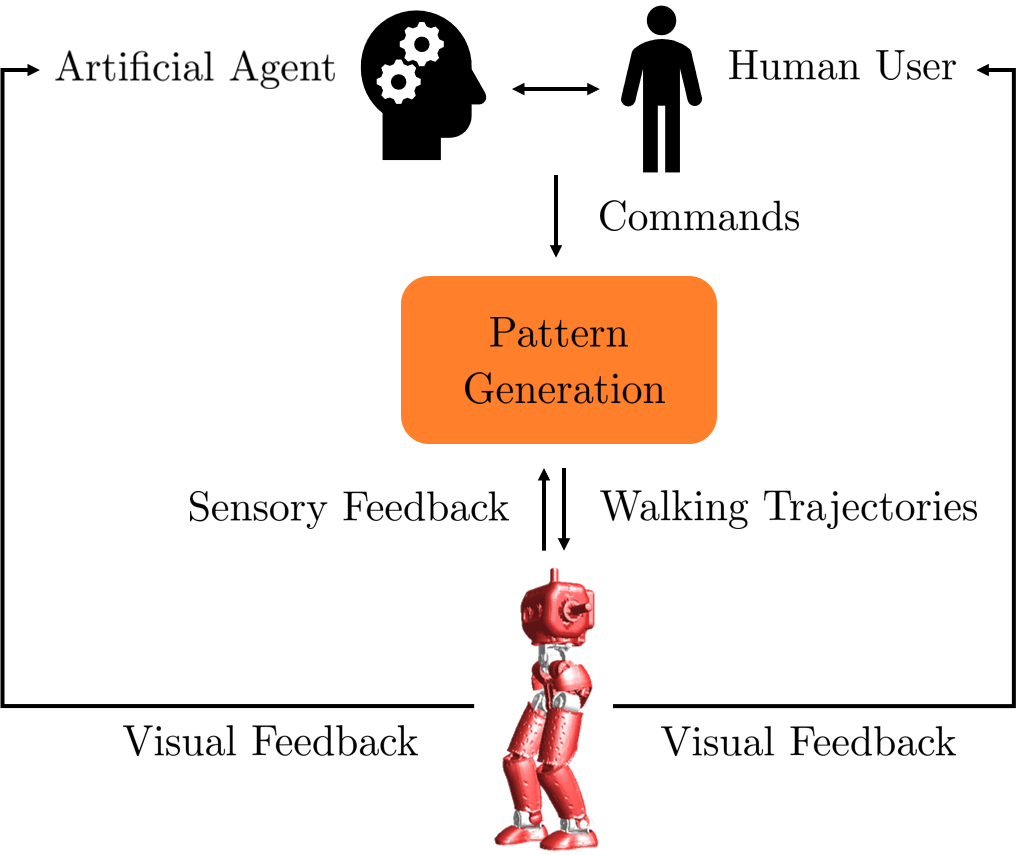
\includegraphics[scale=.5]{chapters/02_background/img/control_loop.png}
	\caption{Simplified version of the proposed control loop to navigate the robot with either a human user or an artificial agent. The commands will be given in the form of linear velocities $v_x$, and $v_y$, along the x-, and the y-axis, as well as an angular velocity $\omega_z$ about the z-axis of the robot's coordinates system.}
	\label{fig::2_cl}
\end{figure}
\\
To close the control loop and to steer the robot towards desired goals, whilst avoiding obstacles, requires some sort of high level command that arises from visual feedback. As discussed in section \ref{sec::12_so} - Introduction, there are several ways to achieve this, among them human users. Of particular interest to us are novel methods that evolved from the toolbox of machine learning techniques, as they decrease the computational cost into non existence. Let alone this fact enables us to run them onboard on light weight hardware with low energy usage, which is critical in the domain of humanoid robots. Center to these new methods will be neural nets that we will train on solving the task of autonomous navigation in two different ways. One of which clones the behavior of a human user (sec. \ref{sec::222_bc}), whereas the second presented method (sec. \ref{sec::223_rl}) explores policies and tries to find solutions on its own.
\\\\
As a side note, within the following chapters there will always be made references to the actual implementation of the presented concepts. This shall enable future readers to bridge the gap between theory and application.   % introduction to background
	\FloatBarrier
\section{Humanoid Walking}
\label{sec::21_hw}
To get started with and to understand the presented concepts that generate dynamically balanced walking trajectories, we shall have a look at figure \ref{fig::2_cl} once more. The pattern generation therein (orange box), consists of four main building blocks: Forward kinematics, nonlinear model predictive control (NMPC), interpolation, and inverse kinematics. The relation between these four building blocks is shown in fig. \ref{fig::21_pg}.
\begin{figure}[h!]
	\centering
	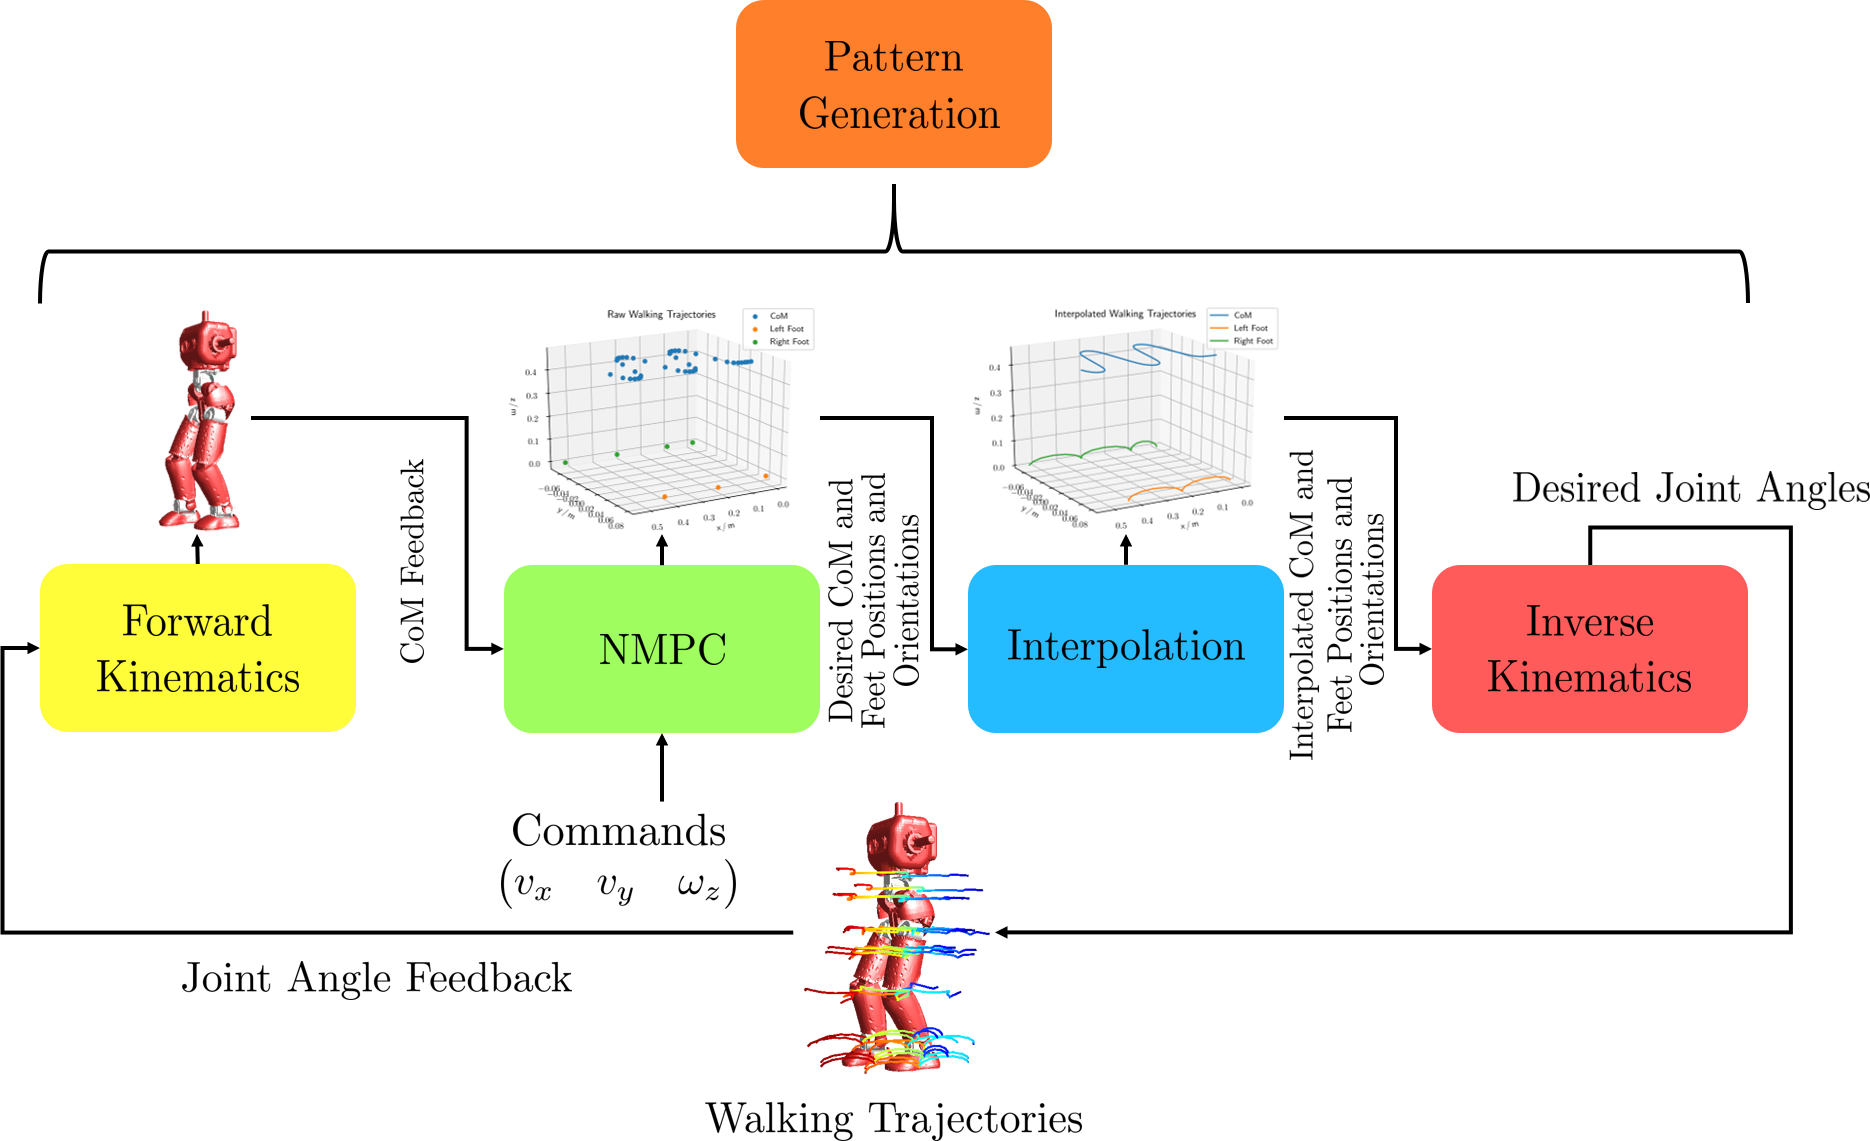
\includegraphics[scale=.5]{chapters/02_background/img/pattern_generation.png}
	\caption{Building blocks of the pattern generation. To understand the greater picture, a connection can be drawn to fig. \ref{fig::2_cl}, where the orange box represents the one shown in this figure.}
	\label{fig::21_pg}
\end{figure}
The natural entry point, to this otherwise closed control loop, is given by the commands that enter the nonlinear model predictive control. Commands are passed in the form of a desired velocity $\mathbf{v}_\text{ref}$ that the robot's center of mass (CoM) shall satisfy optimally according to a cost function that also takes dynamic balance and a smooth motion into account. The future desired positions and orientations for the CoM and the feet then result from the solution to a sequentially quadratic problem that tries to minimize this cost function. The balance criteria within this problem formulation is based upon the zero moment point (ZMP) around which the whole control framework is built. It is only by simplifying the robot's model that we can solve the optimal control problem in real time. Therefore, we assume the robot to be a linear inverted pendulum, for which we have a well-defined analytical relation between the CoM and the ZMP. The minimization of the distance between the analytical expression of the ZMP and the foot placement results in the desired dynamic balance. As shown in fig. \ref{fig::21_pg}, the desired CoM and the feet positions and orientation, as they are obtained from the NMPC, are sparsely distributed in space. Moreover, there is neither information about how the feet shall move along the z-axis, nor along the x-, and y-axis, but only where they should be placed in the x-y-plane. Therefore, as the subsequent step to the NMPC, we need to add an interpolation. The interpolation interpolates the trajectories of the CoM to obtain a finer sampling time. Additionally, the movement of the feet in the x-, y-, and z-direction, as well as their orientation, is computed by polynomials that we require to satisfy the initial and end conditions of the foot placement. Put together, the nonlinear model predictive control and the interpolation between the resulting subsequent solutions for the positions and orientation of both, the CoM and the feet, describe dynamically balanced trajectories, given that the humanoid robot of interest resembles the physics of an inverted pendulum. Now to bridge the gap between dynamically balanced trajectories in Cartesian space, and a humanoid robot that satisfies them with its CoM and its feet, the inverse kinematics problem needs to be addressed. The inverse kinematics, which follow immediately after the interpolation step, take the positions and orientations of the CoM and the feet as constraints and find a composite of joint angles that fulfil them. The continuity of subsequent solutions is therein assured by initializing the inverse kinematics with the previous solution. Resulting joint angles, once passed to the humanoid, then result in walking trajectories, as indicated in fig. \ref{fig::21_pg} by the colored lines at the joints of the robot. Due to the inherent mismatch of the robot's physics from that of an inverted pendulum, as well as other effects like friction, there is a chance that the desired joint angles differ from the achieved ones. To compensate for the discrepancy, the last building block of the pattern generation is the feedback of the measured CoM to the NMPC. The CoM is computed by reading out the achieved joint angles, so that the forward kinematics can be utilized to determine the positions and orientations of the humanoid's links in space, and therefore the CoM.
\\\\
As already highlighted in the previous paragraph, special attention has to be given to the zero moment point, since it defines the central concept of the presented pattern generation. We therefore will explain its theoretical foundations, as well as its analytical relationship to the CoM for simplified physical models, and ways to measure it with force torque sensors in the section that lies ahead - Zero Moment Point.





    % short overview of humanoid walking
	\FloatBarrier
\subsection{Zero Moment Point}
\label{sec::211_zmp}
The key metric in this work, for the generation of a dynamically balanced gait, is the zero moment point. The concept was first introduced by Miomir Vukobratovi\'{c} and Davor Juri\v{c}i\'{c} in 1968 \cite{vukobratovic1968contribution}\cite{vukobratovic1969contribution} and first utilized 1984 to generate walking trajectories for the WL-10RD robot \cite{yamaguchi1993development}. The most intuitive understanding for the ZMP arises by thinking about the realization of the simplest arbitrary possible walking motion for which a humanoid robot will not fall. This motion is achieved by ensuring the feet's whole area, and not only the edge, is in contact with the ground \cite{vukobratovic2004zero}, or put in other words, we require the robot not to rotate about its feet edges. This constraint can be met by having a reaction force $\bm{F}_r$ between the foot and the ground, which compensates for all external moments $\bm{M}_x$, and $\bm{M}_y$ around the x-, and y-axis at any time (fig. \ref{fig::211_zmp}).
\begin{figure}[h!]
	\centering
	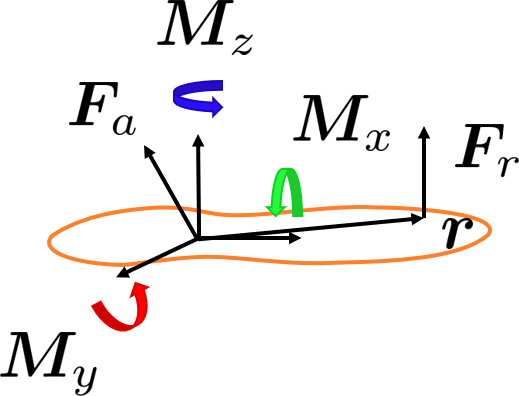
\includegraphics[scale=.5]{chapters/02_background/img/zero_moment_point.png}
	\caption{Forces acting on the sole.}
	\label{fig::211_zmp}
\end{figure}
The point $\bm{r}$, at which the reaction force acts, is physically only meaningful if it lies within the support polygon of the foot. Not only can it not exist outside of the support polygon, since there was no point of interaction between the foot and the ground then, but also was the robot to overturn under these circumstances. Therefore, the ZMP is defined as that point on the ground at which the net moment of the inertial forces has no component along the horizontal axes \cite{hirai1998development}\cite{dasgupta1999making}. We now came to appreciate the importance of the support polygon for the definition of the zero moment point. 
\begin{figure}[h!]
	\centering
	
\includegraphics[scale=.5]{chapters/02_background/img/support_polygon.png}
	\caption{Full support polygon, and the resulting support polygon with security margin (dashed lines).}
	\label{fig::211_support_polygon}
\end{figure}
The support polygon is defined as the convex hull of all contact points of the feet with the ground, so the minimal number of points to fully contain all of them. As the most restrictive case for balance, in this work we will only consider the support polygon of one foot at a time. Since the convex hull of a foot is well described by a rectangle, we only rely on the foot width (\href{https://github.com/mhubii/nmpc_pattern_generator/blob/bc79a6d4f9bcfd3794146355af44429f5b7a9fe0/libs/pattern_generator/configs.yaml#L14}{\underline{link}}), and foot length (\href{https://github.com/mhubii/nmpc_pattern_generator/blob/bc79a6d4f9bcfd3794146355af44429f5b7a9fe0/libs/pattern_generator/configs.yaml#L15}{\underline{link}}) to fully describe it. Also, to ensure that the zero moment point never comes close to the edges of the feet and therefore to provide balance, we define a security margin to their boarders (\href{https://github.com/mhubii/nmpc_pattern_generator/blob/bc79a6d4f9bcfd3794146355af44429f5b7a9fe0/libs/pattern_generator/configs.yaml#L3}{\underline{link}}). The respective values are robot specific and can be set in the configurations file by following the provided links.
\\\\
As already pointed out, within this work, we will use a simplified physical model of the humanoid solve the optimal control problem in real time. We will deal with this approximation in the following paragraph - Zero Moment Point of a Linear Inverted Pendulum.
\FloatBarrier
\subsubsection{Zero Moment Point of a Linear Inverted Pendulum}
Dynamically balanced walking trajectories can be generated by simplifying the dynamics of humanoid robots to those of a linear inverted pendulum \cite{kajita2003biped}. A rigorous derivation for the analytic relation between the center of mass and the zero moment point of a linear inverted pendulum can be found in \cite{kajita2014introduction}, but for the sake of simplicity we rather explain the physics in terms of cutting forces, for which a short introduction can be found in the summary of the lecture Robotics 1 (\href{https://drive.google.com/file/d/1aN1ujXTOlHzO2kLPK7TQRkWfdY-pGzUF/view}{\underline{link}}). 
\begin{figure}[h!]
	\centering
	\subcaptionbox{}%
	[.4\linewidth]{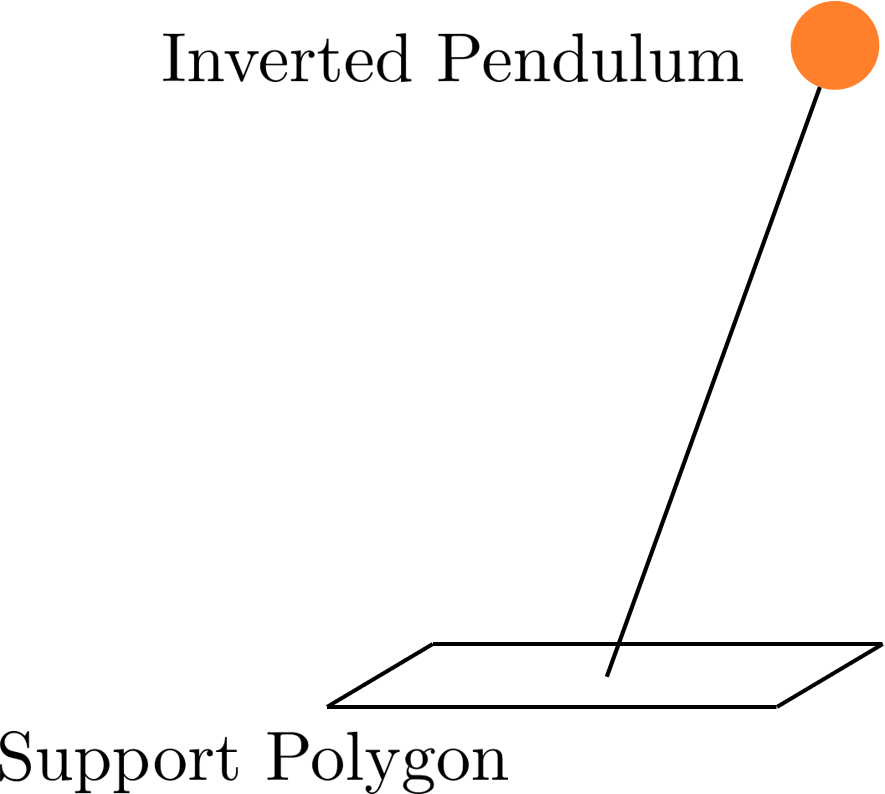
\includegraphics[scale=.3]{chapters/02_background/img/inverted_pendulum.png}}
	\subcaptionbox{}%
	[.4\linewidth]{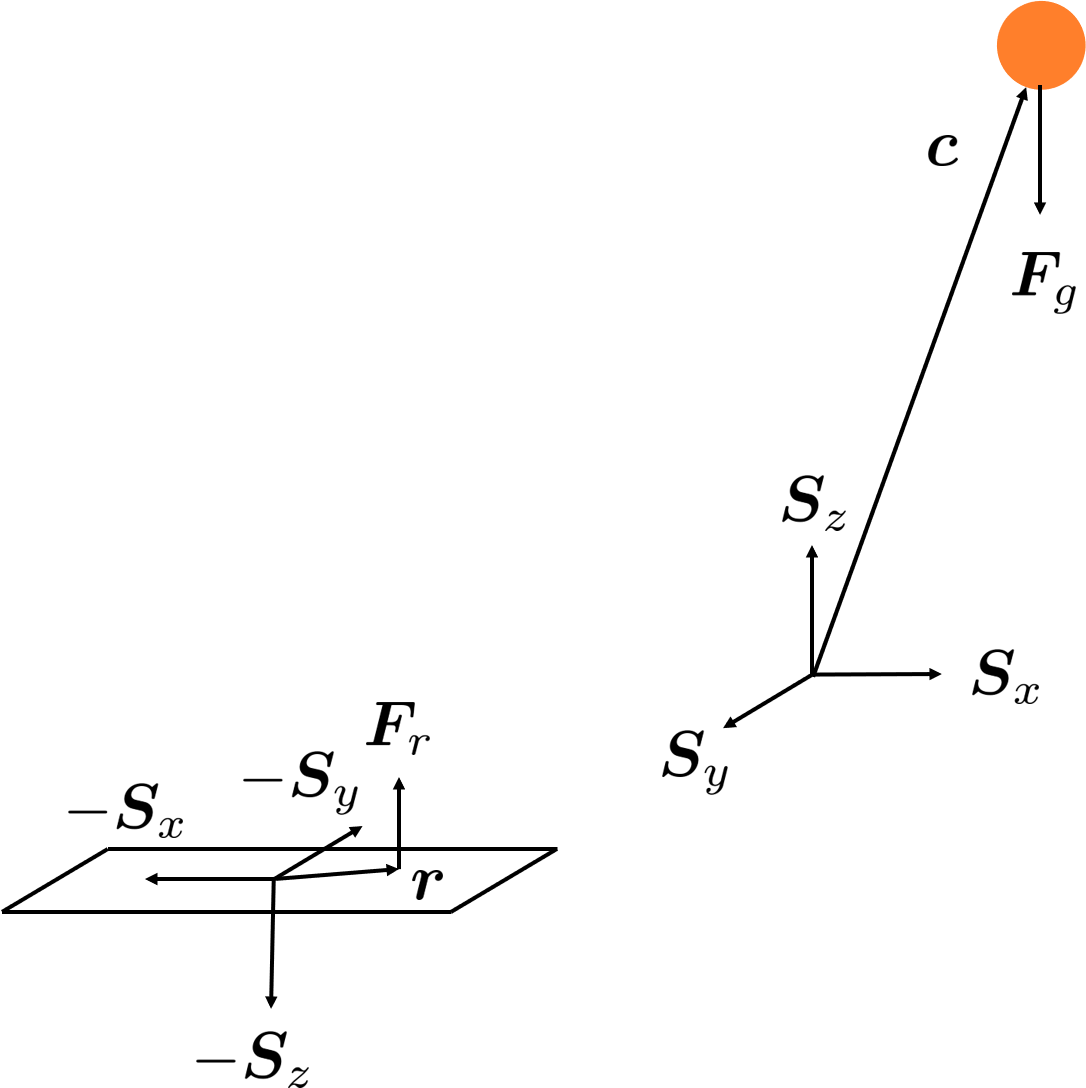
\includegraphics[scale=.3]{chapters/02_background/img/inverted_pendulum_free_body_diagram.png}}
	\caption{Linear inverted pendulum with a support polygon (a), and the corresponding free body diagram with cutting forces $\bm{S}_{x/y/z}$ (b).}
	\label{fig::211_lip}
\end{figure}
The system of interest is shorty depicted in figure \ref{fig::211_lip}. We assume the support polygon of the shown linear inverted pendulum to have zero mass. By introducing cutting forces $\bm{S}_{x/y/z}$ for each degree of freedom in which the motion of the linear inverted pendulum is restricted, we obtain the free body diagram (fig. \ref{fig::211_lip}), for which the acting forces are
\begin{align}
	m\ddot{\bm{c}} &=\quad\bm{S} - \bm{F}_g 
	\label{eq::211_pendulum_force} \\
	\bm{0} &= -\bm{S}+\bm{F}_r
	\label{eq::211_support_polygon_force}
\end{align}
where $\bm{S}=\bm{S}_x+\bm{S}_y+\bm{S}_z$. The respective moments, since we do not take any inertias into account, are given by
\begin{align}
	\bm{0} &= (\bm{0}-\bm{c})\times\bm{S} + \bm{M} 
	\label{eq::211_pendulum_moment}\\	
	\bm{0} &= (\bm{r}-\bm{0})\times\bm{F}_r - \bm{M}
	\label{eq::211_support_polygon_moment}	
\end{align}
where the transfer of the moment $\bm{M}$ may for example be induced by friction. If we replace $\bm{S}=\bm{F}_r$ from eq. \ref{eq::211_support_polygon_force}, equations \ref{eq::211_pendulum_moment} and \ref{eq::211_support_polygon_moment} yield 
\begin{align}
	\bm{0} = (\bm{r}-\bm{c})\times\bm{S} = \begin{pmatrix}
	\quad(r_y - c_y)S_z - (r_z - c_z)S_y \\
	-(r_x - c_x)S_z + (r_z - c_z)S_x \\
	\quad(r_x - c_x)S_y - (r_y - c_y)S_x
	\end{pmatrix}
	\label{eq::211_momentum_transfer}
\end{align}
Since our goal is to have a robot that does not fall, we want to achieve that the acceleration along the z-axis becomes zero, hence $\ddot{c}_z=0$. Given this assumption, we can infer from eq. \ref{eq::211_pendulum_force} that $S_z=mg$, as well as $S_x = \ddot{c}_xm$, and $S_y = \ddot{c}_ym$. Furthermore, our foot shall not lift off the floor, and therefore we have $r_z=0$. If we take these assumptions and plug them into the first to rows of eq. \ref{eq::211_momentum_transfer}, we find
\begin{align}
	r_x &= c_x - c_z\frac{\ddot{c}_x}{g}
	\label{eq::211_zmp_x}\\
	r_y &= c_y - c_z\frac{\ddot{c}_y}{g}
	\label{eq::211_zmp_y}
\end{align}
Therein, $r_x$, and $r_y$ are the x-, and y-coordinates of the zero moment point, given the assumption of a linear inverted pendulum. We can see that the position if dependent on the height of the point mass, which is in turn dependent on the robot. The specific values can be set in the configurations file (\href{https://github.com/mhubii/nmpc_pattern_generator/blob/bc79a6d4f9bcfd3794146355af44429f5b7a9fe0/libs/pattern_generator/configs.yaml#L27}{\underline{link}}).
\\\\
We have now found a simple analytic expression for the relationship of the zero moment point and the center of mass, which will help us to formulate an optimal control problem that we can solve in real time. This simplification is of course only true to some extend, and we need to find a way to verify its accuracy. The easiest way to do so is to measure the real zero moment point. We will further elaborate on this within the next paragraph - Measurement of the Zero Moment Point, and we will derive a method that only relies on force torque sensors in the ankle.
\FloatBarrier
\subsubsection{Measurement of the Zero Moment Point}
There are several methods that enable us to measure the position of the zero moment point, among them the utilization of pressure sensitive soles, as outlined in \cite{kajita2014introduction}. Furthermore, there exist approximate approaches that involve the knowledge of all acting external forces \cite{huang2001planning}, which can for example be obtained from unconstrained inverse dynamics \cite{michel2017dynamic}. Since we can rely on measurements of force torque sensors that are located at the ankles, we will infer the position of the zero moment point from them \cite{kajita2014introduction}. 
\begin{figure}[h!]
	\centering
	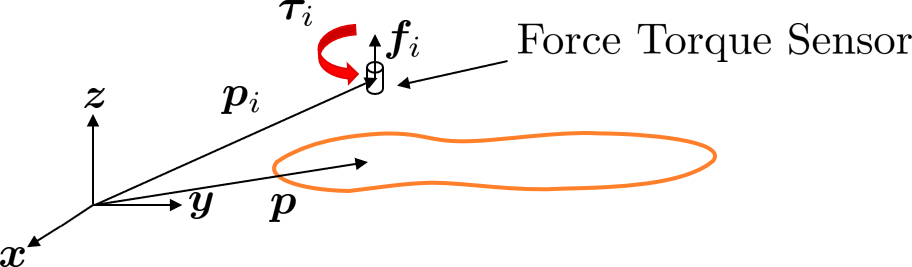
\includegraphics[scale=.5]{chapters/02_background/img/ft_sensor.png}
	\caption{Force torque sensors at the foot's ankle.}
	\label{fig::211_force_torque}
\end{figure}
If we consider the force torque sensor to be located at position $\bm{p}_i$ (fig. \ref{fig::211_force_torque}), then we can obtain the moment about any point $\bm{p}$ according to eq. \ref{eq::211_moment}.
\begin{align}
	\bm{\tau}(\bm{p}) = (\bm{p}_i-\bm{p})\times \bm{f}_i + \bm{\tau}_i
	\label{eq::211_moment}
\end{align}
by definition, the moment about the zero moment point vanishes along the horizontal axes, therefore we can then set $\tau_x = \tau_y = 0$ in eq. \ref{eq::211_moment} and then solve for the position to obtain the zero moment point (eq. \ref{eq::211_x_pos_zmp} and \ref{eq::211_y_pos_zmp}).
\begin{align}
	p_x &= \frac{\left[-\tau_{i,y}-(p_{i,z}-p_z)f_{i,x}+p_{i,x}f_{i,z}\right]}{f_{i,z}}
	\label{eq::211_x_pos_zmp}\\
	p_y &= \frac{\left[-\tau_{i,x}-(p_{i,z}-p_z)f_{i,y}+p_{i,y}f_{i,z}\right]}{f_{i,z}}
	\label{eq::211_y_pos_zmp}
\end{align}
If we further choose our coordinate system to lie along the z-axis of the force torque sensor (fig. ...), we can simplify equations \ref{eq::211_x_pos_zmp} and \ref{eq::211_y_pos_zmp} to find
\begin{align}
	p_x &= \frac{(-\tau_{i,y}-f_{1,x}d)}{f_{1,z}} 
	\label{eq::211_x_pos_zmp_simp}\\
	p_y &= \frac{(\tau_{i,x}-f_{1,y}d)}{f_{1,z}}
	\label{eq::211_y_pos_zmp_simp}
\end{align}
We can use equations \ref{eq::211_x_pos_zmp_simp} and \ref{eq::211_y_pos_zmp_simp} to determine the position of the zero moment point for the left and the right foot with respect to coordinates frames that are attached to the respective foot. These circumstances change once not only one, but both feet are in contact with the ground. What still holds true, in the case of a dynamically balanced gait, is the fact that the positions which we just obtained from equations \ref{eq::211_x_pos_zmp_simp} and \ref{eq::211_y_pos_zmp_simp} represent points where the interaction of the robot with the environment can solely be described by a single force along the z-axis. All other forces or torques cancel out. Therefore, to determine the position of the zero moment point for the double support phase, we need to modify equation \ref{eq::211_moment} slightly. This yields 
\begin{align}
	\bm{\tau}(\bm{p}) = \sum_{i\in\{L, R\}} (\bm{p}_i - \bm{p})\times\bm{f}_i
	\label{eq::211_moment_ds}
\end{align}
where the individual torques are now zero and the only forces $\bm{f}_i$ that exist between the robot and the environment can be described by the z-component which are measured at the ankles' force torque sensors. Yet again, to obtain the position of the zero moment point, we have to set the x-, and y-components of the torque in equation \ref{eq::211_moment_ds} to zero and find
\begin{align}
	p_x &= \frac{\sum_{i\in\{L, R\}}p_{i,x}f_{i,z}}{\sum_{i\in\{L, R\}}f_{i,z}} \\
	p_y &= \frac{\sum_{i\in\{L, R\}}p_{i,y}f_{i,z}}{\sum_{i\in\{L, R\}}f_{i,z}}
\end{align}
These expressions of course only hold true in a shared coordinate system and therefore we need to transform the position of the zero moment point which we obtained from equations \ref{eq::211_x_pos_zmp_simp} and \ref{eq::211_y_pos_zmp_simp} to the world frame. Finally, we can write down the formulation for the zero moment point which holds equally true for the single and double support phase
\begin{align}
	p_x &= \frac{p_{R,x}f_{R,z}+p_{L,x}f_{L,z}}{f_{R,z}+f_{L,z}} 
	\label{eq::211_double_zmp_x} \\
	p_y &= \frac{p_{R,y}f_{R,z}+p_{L,y}f_{L,z}}{f_{R,z}+f_{L,z}}
	\label{eq::211_double_zmp_y}
\end{align}
At this point we are now equipped with a general understanding for the zero moment point, as well as with the knowledge of simplified models to compute it analytically, and a method to measure it so that we can evaluate the performance of a potential pattern generator which is based upon the zero moment point. Therefore, in the next chapter - Nonlinear Model Predictive Control, we will try to understand a method that allows us to generate dynamically balanced center of mass and feet trajectories, which satisfy the just introduced concepts optimally, given a weighting factor.
  % zero moment point
	\FloatBarrier
\subsection{Nonlinear Model Predictive Control}
\label{sec::212_nmpc}
At the heart of nonlinear model predictive control stands sequential quadratic programming. Before we come to the actual problem formulation, we need to understand how sequential quadratic programming can be used to solve nonlinear optimization problems. We will then come to recognize that if we can find a canonical formulation of our problem, it will become possible to apply sequential quadratic programming to it. The next paragraph - Sequential Quadratic Programming, will therefore shortly introduce the reader to the desired method that will be used to solve the  nonlinear optimization problem, while the subsequent paragraph - Canonical Formulation of Nonlinear Model Predictive Control, will then explain how to fit humanoid walking into this framework.
\FloatBarrier
\subsubsection{Sequential Quadratic Programming}
\label{sec::212_sqp}
Sequential quadratic programming is a powerful concept to solve nonlinearly constrained optimization problems. The nonlinear programming problem to be solved is of the form
\begin{align}
	\min_{\bm{x}}\, &\frac{1}{2}f(\bm{x})
	\label{eq::212_objective}\\
	\text{subject to: } &\bm{h}(\bm{x}) = \bm{0}\\
	&\bm{g}(\bm{x}) \leq \bm{0},
\end{align}
where $f:\,\mathbb{R}^N\rightarrow\mathbb{R}$, $\bm{h}:\,\mathbb{R}^N\rightarrow\mathbb{R}^M$, and $\bm{g}:\,\mathbb{R}^N\rightarrow\mathbb{R}^P$ \cite{boggs1995sequential}. These problems arise in a variety of applications in science and include quadratic problems as special cases. The great strength of sequential quadratic programming is its ability to solve problems with nonlinear constraints, and its basic idea is to model nonlinear programming at an approximate solution $\bm{x}_k$ by a quadratic subproblem, so to find a solution to this subproblem, in order to construct a better approximation $\bm{x}_{k+1}$. Now given an objective function $f(\bm{x})$ represents a sum of squares, the problem at hand turns into a nonlinear least squares problem, and the minimization can be expressed in terms of a Gauss-Newton method \cite{schittkowski1988solving}. That is, given an objective function $f(\bm{x}) = \bm{F}(\bm{x})^T\bm{F}(\bm{x})$, where $\bm{F}=\left(f_1,...,f_l\right)^T$, we can apply a quasi Gauss-Newton method as follows
\begin{align}
	\nabla^2f(\bm{x})\Delta\bm{x} + \nabla f(\bm{x}) = 0,
	\label{eq::212_quasi_gn}
\end{align}
where the gradient and the Hessian matrix are given as
\begin{align}
	\nabla f(\bm{x}) &= \nabla \bm{F}(\bm{x})\bm{F}(\bm{x}) \\
	\nabla^2 f(\bm{x}) &= \nabla \bm{F}(\bm{x})\nabla\bm{F}(\bm{x})^T + \bm{B}(\bm{x}).
\end{align}
Therein, $\bm{B}(\bm{x}) = \sum_1^lf_i(\bm{x})\nabla^2f_i(\bm{x})$. If we are now sufficiently close to an optimal solution $\bm{x}^*$, such that $\bm{F}(\bm{x}^*) = \left(f_1(\bm{x}^*),...,f_l(\bm{x}^*)\right)^T=\bm{0}$, we can neglect $\bm{B}(\bm{x^*})$, which turns equation \ref{eq::212_quasi_gn} into the previously stated Gauss-Newton minimization problem
\begin{align}
	\min_{\Delta\bm{x}}\,||\nabla\bm{F}(\bm{x_k})^T\Delta\bm{x}+\bm{F}(\bm{x}_k)||^2_2,
	\label{eq::212_gn_min}
\end{align}
where a new iterate is obtained by $\bm{x}_{k+1}=\bm{x}_k + \alpha_k\Delta \bm{x}$ with an appropriate step length parameter $\alpha_k$. This is because equation \ref{eq::212_quasi_gn} defines the normal equations of equation \ref{eq::212_gn_min}. The presented approach assures quadratic convergence, when starting sufficiently close to an optimal solution. Within the next section, we will understand how to apply this concept to control the zero moment point of a linear inverted pendulum in a balanced manner.
\FloatBarrier
\subsubsection{Canonical Formulation of Nonlinear Model Predictive Control}
Not only do we want to keep a humanoid robot dynamically balanced in terms of the zero moment point, which we derived in equations \ref{eq::211_zmp_x} and \ref{eq::211_zmp_y}, but further do we want to assure this for future time steps that are yet ahead. The underlying model predictive control got first introduced in \cite{kajita2003biped}, and is based upon a linear time stepping scheme, which integrates the current jerk of the center of mass iteratively, so to estimate its future position. We will briefly present it in the following paragraph - Linear Time Stepping Scheme.
\FloatBarrier
\subsubsection{Linear Time Stepping Scheme}
Suppose that the center of mass' jerk $\dddot{c}_k$ at time step $t_k$ is constant, then given the current acceleration $\ddot{c}_k$, we can obtain the acceleration $\ddot{c}_{k+1}$ at time step $t_{k+1}$ by simple integration. We can do the same for the velocity and position and therefore obtain
\begin{align}
	c_{k+1} &= \frac{T^3}{6}\dddot{c}_k+\frac{T^2}{2}\ddot{c}_k+T\dot{c}_k+c_k\\
	\dot{c}_{k+1} &= \frac{T^2}{2}\dddot{c}_k+T\ddot{c}_k+\dot{c}_k\\
	\ddot{c}_{k+1} &= T\dddot{c}_{k} + \ddot{c}_k,
\end{align}
where $T = t_{k+1}-t_k$. We can rewrite this in compact form by
\begin{align}
	&\bm{c}_{k+1} = \bm{A}\bm{c}_k + \bm{B}\dddot{c}_k \\
	&\bm{c}_{k+1} = \begin{pmatrix}
	c_{k+1} \\
	\dot{c}_{k+1} \\
	\ddot{c}_{k+1}
	\end{pmatrix},\,\,
	\bm{A} = \begin{pmatrix}
	1 & T & \frac{T^2}{2} \\
	0 & 1 & T \\
	0 & 0 & 1
	\end{pmatrix},\,\,
	\bm{B} = \begin{pmatrix}
	\frac{T^3}{6} \\
	\frac{T^2}{2} \\
	T
	\end{pmatrix}
	\label{eq::212_ltss}
\end{align}
Now by recursion, one obtains the positions, velocities, and accelerations for $n$ future time steps via
\begin{align}
	\bm{c}_{k+n} = \bm{A}^n\bm{c}_k\sum_{i=1}^n \bm{A}^{i-1}\bm{B}\dddot{c}_{k+n-i},
	\label{eq::212_preview}
\end{align}
where $n\in[1,N]$. Altogether we have
\begin{align}
	\bm{A}^n = \begin{pmatrix}
	1 & nT & n^2\frac{T^2}{2} \\
	0 & 1 & nT \\
	0 & 0 & 1
	\end{pmatrix},\,\,
	\bm{A}^n\bm{B} = \begin{pmatrix}
	(1+3n+3n^2)T^3/6 \\
	(1+2n)T^2/2 \\
	T
	\end{pmatrix}.
	\label{eq::212_preview_mat}
\end{align}
The amount of time $NT$ that we predict into the future, is what we call the preview horizon. If we now concatenate the single entries of $\bm{c}_{k+n}$ for all $n\in[1,N]$ into one expression, we can relate the initial states $\bm{c}_k$ (\href{https://github.com/mhubii/nmpc_pattern_generator/blob/5a213044c927dc6aac9f7e32ce1e5fb472cd67bb/libs/pattern_generator/include/pattern_generator/base_generator.h#L140}{\underline{link}}) to the states on the preview horizon in an even more compact form. With the concatenations (\href{https://github.com/mhubii/nmpc_pattern_generator/blob/5a213044c927dc6aac9f7e32ce1e5fb472cd67bb/libs/pattern_generator/include/pattern_generator/base_generator.h#L146}{\underline{link}})
\begin{align}
	\bm{C}_{k+1}=\begin{pmatrix}
	c_{k+1}\\
	\vdots\\
	c_{k+N}
	\end{pmatrix},\,\,
	\dot{\bm{C}}_{k+1}=\begin{pmatrix}
	\dot{c}_{k+1}\\
	\vdots\\
	\dot{c}_{k+N}
	\end{pmatrix},\,\,
	\ddot{\bm{C}}_{k+1}=\begin{pmatrix}
	\ddot{c}_{k+1}\\
	\vdots\\
	\ddot{c}_{k+N}
	\end{pmatrix},\,\,
	\dddot{\bm{C}}_{k}=\begin{pmatrix}
	\dddot{c}_{k}\\
	\vdots\\
	\dddot{c}_{k+N-1}
	\end{pmatrix},
\end{align}
we obtain (\href{https://github.com/mhubii/nmpc_pattern_generator/blob/5a213044c927dc6aac9f7e32ce1e5fb472cd67bb/libs/pattern_generator/src/base_generator.cpp#L887}{\underline{link}})
\begin{align}
	\bm{C}_{k+1} &= \bm{P}_{ps} \bm{c}_k + \bm{P}_{pu}\dddot{\bm{C}}_k
	\label{eq::212_ckp1}\\
	\dot{\bm{C}}_{k+1} &= \bm{P}_{vs} \bm{c}_k + \bm{P}_{vu}\dddot{\bm{C}}_k
	\label{eq::212_dckp1}\\
	\ddot{\bm{C}}_{k+1} &= \bm{P}_{as} \bm{c}_k + \bm{P}_{au}\dddot{\bm{C}}_k,
	\label{eq::212_ddckp1}
\end{align}
where the new matrices are given by (\href{https://github.com/mhubii/nmpc_pattern_generator/blob/5a213044c927dc6aac9f7e32ce1e5fb472cd67bb/libs/pattern_generator/src/base_generator.cpp#L403}{\underline{link}})
\begin{align}
	\bm{P}_{ps} &= \begin{pmatrix}
	1 & T & T^2/2 \\
	\vdots & & \vdots \\
	1 & nT & n^2T^2/2
	\end{pmatrix},\,\,
	\bm{P}_{pu} = \begin{pmatrix}
	T^3/6 & \dots & 0 \\
	\vdots & \ddots & \vdots \\
	(1+3n+3n^2)T^2/6 & \dots & T^3/6
	\end{pmatrix} \\
	\bm{P}_{vs} &= \begin{pmatrix}
	0 & 1 & T \\
	\vdots & & \vdots \\
	0 & 1 & nT
	\end{pmatrix},\,\,
	\bm{P}_{vu} = \begin{pmatrix}
	T^2/2 & \dots & 0 \\
	\vdots & \ddots & \vdots \\
	(1+2n)/T^2/2 & \dots & T^2/2
	\end{pmatrix} \\
	\bm{P}_{as} &= \begin{pmatrix}
	0 & 0 & 1 \\
	\vdots  &  & \vdots \\
	 0 & 0 & 1
	\end{pmatrix},\,\,
	\bm{P}_{au}\begin{pmatrix}
	T & \dots & 0 \\
	\vdots & \ddots & \vdots \\
	T & \dots & T
	\end{pmatrix}.
\end{align}
If we now additionally consider the relation of the zero moment point and the center of mass, which we obtained earlier in equations \ref{eq::211_zmp_x} and \ref{eq::211_zmp_y}, we can further relate the current center of mass state to the zero moment point on the preview horizon by (\href{https://github.com/mhubii/nmpc_pattern_generator/blob/5a213044c927dc6aac9f7e32ce1e5fb472cd67bb/libs/pattern_generator/include/pattern_generator/base_generator.h#L219}{\underline{link}})
\begin{align}
	\bm{Z}_{k+1} &= \bm{C}_{k+1} - \frac{c_z}{g}\ddot{\bm{C}}_{k+1} \\
	&= \left(\bm{P}_{ps}-\frac{c_z}{g}\bm{P}_{as}\right)\bm{c}_k + \left(\bm{P}_{pu}-\frac{c_z}{g}\bm{P}_{au}\right)\ddddot{\bm{C}}_k = \bm{P}_{zs} \bm{c}_k + \bm{P}_{zu}\dddot{\bm{C}}_k,
	\label{eq::212_zmp}
\end{align}
where the new matrices are given by (\href{https://github.com/mhubii/nmpc_pattern_generator/blob/5a213044c927dc6aac9f7e32ce1e5fb472cd67bb/libs/pattern_generator/src/base_generator.cpp#L420}{\underline{link}})
\begin{align}
	\bm{P}_{zs} &= \begin{pmatrix}
	1 & T & T^2/2 - c_z/g \\
	\vdots & & \vdots \\
	1 & nT & n^2T^2/2 - c_z/g
	\end{pmatrix} \\ 
	\bm{P}_{zu} &= \begin{pmatrix}
	T^3/6 - Tc_z/g & \dots & 0 \\
	\vdots & \ddots & \vdots \\
	(1+3n+3n^2)T^3/6 - Tc_z/g & \dots & T^3/6-Tc_z/g
	\end{pmatrix}.
\end{align}
The expressions for the preview horizon now allow us to formulate an objective function that takes the robot's dynamic balance for future time steps into account, which in turn results in actions being taken that already take future predictions of the system's dynamics into account. The cost function will be described in the next section - The Objective Function.
\FloatBarrier
\subsubsection{The Objective Function}
To create an objective function, as the one already outlined in section \ref{sec::212_sqp}, we put together squared $L^2$-norm objectives, which account for a desired reference center of mass velocity $\dot{\bm{C}}_{k+1}^\text{ref}$, a balanced foot step placement $\textbf{F}_{k+1}$ close to the zero moment point $\bm{Z}_{k+1}$, and a smooth motion for which the center of mass jerk $\dddot{\bm{C}}_{k+1}$ enters as a regularization. The objective function itself is similar to the one first introduced in \cite{herdt2010online}, but additionally takes the center of mass' rotation around the z-axis into account, and it can be written down as follows
\begin{align}
	\min_{\bm{U}_k} &\frac{\alpha}{2}||\dot{\bm{C}}^x_{k+1} - \dot{\bm{C}}_{k+1}^{x,\text{ref}}||_2^2 + \frac{\alpha}{2}||\dot{\bm{C}}^y_{k+1} - \dot{\bm{C}}_{k+1}^{y,\text{ref}}||_2^2 
	\label{eq::212_dcxy}\\
	&\frac{\alpha}{2}||\bm{E}_L\dot{\bm{F}}^{\theta,L}_{k+1} - \dot{\bm{C}}_{k+1}^{\theta,\text{ref}}||_2^2 + 	\frac{\alpha}{2}||\bm{E}_R\dot{\bm{F}}^{\theta,R}_{k+1} - \dot{\bm{C}}_{k+1}^{\theta,\text{ref}}||_2^2 
	\label{eq::212_dftheta} \\
	&\frac{\beta}{2}||\bm{Z}^x_{k+1}-\bm{F}^x_{k+1}||^2_2 + \frac{\beta}{2}||\bm{Z}^y_{k+1}-\bm{F}^y_{k+1}||^2_2 
	\label{eq::212_fxy}\\
	&\frac{\gamma}{2}||\dddot{\bm{C}}_{k+1}^x||^2_2 + \frac{\gamma}{2}||\dddot{\bm{C}}_{k+1}^y||^2_2	
	\label{eq::212_dddcxy}
\end{align}
Before we address the foot placement therein in more detail, we shortly want to highlight that the reference velocities are the commands, which enter the control loop from figure \ref{fig::21_pg}. We set them to be constant over the whole preview horizon and rotate them to the world frame  by considering the robot's current orientation (\href{https://github.com/mhubii/nmpc_pattern_generator/blob/5a213044c927dc6aac9f7e32ce1e5fb472cd67bb/libs/pattern_generator/src/base_generator.cpp#L324}{\underline{link}}). When we consider that the foot cannot move once it is in contact with the ground, it becomes clear that the foot step placement must be very discrete in time. The number of steps $N_f$ that we plan for in advance is simply given by $NT/T_\text{step}$, where we just divide the duration of the preview horizon $NT$ by the time it takes to perform a step $T_\text{step}$. But as already shown in equation \ref{eq::212_zmp}, and used in equation \ref{eq::212_fxy}, we require balance on a finer timescale. We therefore project the foot placement $\tilde{\bm{F}}_k\in\mathbb{R}^{N_f\times1}$ onto the temporal resolution of the center of mass' control variable by introducing the matrices $\bm{v}_{k+1}$, $\bm{V}_{k+1}$, and the current foot position $f_k$, which yields
\begin{align}
	\bm{F}_{k+1} = \bm{v}_{k+1}f_k + \bm{V}_{k+1}\tilde{\bm{F}}_k,
	\label{eq:312_feet}
\end{align}
where $\bm{v}_{k+1}$ is a $N\times1$ matrix, and $\bm{V}_{k+1}$ is a $N\times N_f$ matrix, and they are for example for $N_f = 3$ given by
\begin{align}
	\bm{v}_{k+1} = \begin{pmatrix}
	1 \\ 
	\vdots \\
	1 \\
	0 \\
	\vdots \\
	0 \\
	0 \\
	\vdots \\
	0
	\end{pmatrix},\,\, 
	\bm{V}_{k+1} = \begin{pmatrix}
	0 & 0 & 0\\
	\vdots & \vdots & \vdots \\
	0 & 0 & 0 \\
	0 & 1 & 0 \\
	\vdots & \vdots & \vdots \\
	0 & 1 & 0 \\
	0 & 0 & 1 \\
	\vdots & \vdots & \vdots \\
	0 & 0 & 1
	\end{pmatrix}
\end{align}
As the robot moves, the matrices change, in that the entries of $v_{k+1}$ are being shifted upwards by one index for every time step $T$, while the new entries at the bottom are set to be zero. All entries of $V_{k+1}$ are also shifted upwards, while the bottom right entry is set to one, but further are all entries of $V_{k+1}$ are being shifted to the left once all entries of $\bm{v}_{k+1}$ are zero (\href{https://github.com/mhubii/nmpc_pattern_generator/blob/5a213044c927dc6aac9f7e32ce1e5fb472cd67bb/libs/pattern_generator/src/base_generator.cpp#L740}{\underline{link}}). If all entries of $\bm{v}_{k+1}$ are zero, then $\bm{v}_{k+1}$ is replaced by the second column of $\bm{V}_{k+1}$. For example for $N_f = 2$ and $N=6$  we have
\begin{align}
	\left(
	\begin{array}{c|c}
	\bm{v}_{k+1} & \bm{V}_{k+1}
	\end{array} 
	\right) =
	\left(
	\begin{array}{c|cc}
	1 & 0 & 0 \\
	0 & 1 & 0 \\
	0 & 1 & 0 \\ 
	0 & 1 & 0 \\
	0 & 0 & 1 \\
	0 & 0 & 1
	\end{array}\right) \rightarrow
	\left(
	\begin{array}{c|cc}
	1 & 0 & 0 \\
	1 & 0 & 0 \\
	1 & 0 & 0 \\ 
	0 & 1 & 0 \\
	0 & 1 & 0 \\
	0 & 1 & 0
	\end{array}\right) \rightarrow
	\left(
	\begin{array}{c|cc}
	1 & 0 & 0 \\
	1 & 0 & 0 \\
	0 & 1 & 0 \\ 
	0 & 1 & 0 \\
	0 & 1 & 0 \\
	0 & 0 & 1
	\end{array}\right)
\end{align}
Now to ensure the rotation of the center of mass, we introduce equation \ref{eq::212_dftheta} to the objective function. The matrices $\bm{E}_{L/R}$ therein ensure that only the foot, which is currently not touching the ground, is rotated, the rotational velocity of the center of mass itself is then obtained by averaging over the left and the right foot. Hence $\bm{E}_{L/R}$ take the form (\href{https://github.com/mhubii/nmpc_pattern_generator/blob/5a213044c927dc6aac9f7e32ce1e5fb472cd67bb/libs/pattern_generator/src/base_generator.cpp#L1281}{\underline{link}})
\begin{align}
	\bm{E}_L = \begin{pmatrix}
	1&&&&&&&& \\
	&\ddots&&&&&&& \\
	&&1&&&&&& \\
	&&&0&&&&& \\
	&&&&\ddots&&&& \\
	&&&&&0&&& \\
	&&&&&&1&& \\
	&&&&&&&\ddots& \\
	&&&&&&&&1 \\
	\end{pmatrix},\,\,
	\bm{E}_R = \bm{1} - \bm{E}_L
\end{align}
The diagonal entries therein just take the same form as a single column of $\bm{V}_{k+1}$, all other entries are zero. If we now take equations \ref{eq::212_dcxy}-\ref{eq::212_dddcxy}, and replace $\dot{\bm{C}}_{k+1}^{x/y}$, as well as $\dot{\bm{F}}_{k+1}^{\theta,L/R}$, by equation \ref{eq::212_dckp1}, and insert equation \ref{eq::212_zmp} into the zero moment point on the preview horizon $\bm{Z}_{k+1}$, we obtain following relation (\href{https://github.com/mhubii/nmpc_pattern_generator/blob/5a213044c927dc6aac9f7e32ce1e5fb472cd67bb/libs/pattern_generator/src/nmpc_generator.cpp#L145}{\underline{link}})
\begin{align}
	\min_{\bm{U}_k} &\frac{1}{2}\bm{U_k}^T\bm{Q}_k\bm{U}_k + \bm{p}_k^T\bm{U}_k
	\label{eq::212_canqp} \\
	& \bm{U}_k = \begin{pmatrix}
	\bm{U}^{xy}_k & \bm{U}^\theta_k
	\end{pmatrix}^T\\	
	&\bm{U}^{xy}_k = \begin{pmatrix}
	\dddot{\bm{C}}^x_k & \tilde{\bm{F}}_k^x & \dddot{\bm{C}}_k^y & \tilde{\bm{F}}_k^y
	\end{pmatrix}^T\\
	&\bm{U}^\theta_k = \begin{pmatrix} \dddot{\bm{F}}_k^{\theta, L} & \dddot{\bm{F}}_k^{\theta, R} 
	\end{pmatrix}^T \\
	&\bm{Q}_k = \begin{pmatrix}
	\bm{Q}_k^{x} & \bm{0} & \bm{0} & \bm{0} \\
	\bm{0} & \bm{Q}_k^{y} & \bm{0} & \bm{0} \\
	\bm{0} & \bm{0} & \bm{Q}_k^L & \bm{0} \\ 
	\bm{0} & \bm{0} & \bm{0} & \bm{Q}_k^R
	\end{pmatrix}
	\label{eq::212_qk}\\
	& \bm{Q}_k^x = \bm{Q}_k^y = \begin{pmatrix}
		\alpha\bm{P}_{vu}^T\bm{P}_{vu}+\beta\bm{P}_{zu}^T\bm{P}_{zu}+\gamma\bm{1} & -\beta\bm{P}_{zu}^T\bm{V}_{k+1} \\
		-\beta\bm{V}_{k+1}^T\bm{P}_{zu} & \beta\bm{V}_{k+1}^T\bm{V}_{k+1}
	\end{pmatrix}\\
	& \bm{Q}_k^{L/R} = \begin{pmatrix}
		\alpha\bm{P}_{vu}^T\bm{E}_{L/R}^T\bm{E}_{L/R}\bm{P}_{vu}
	\end{pmatrix}\\
	&\bm{p}_k = \begin{pmatrix}
		\bm{p}_k^x \\
		\bm{p}_k^y \\
		\bm{p}_k^{L} \\
		\bm{p}_k^{R}
	\end{pmatrix} \\
	& \bm{p}_k^{x/y} = \begin{pmatrix}
		\alpha\bm{P}_{vu}^T(\bm{P}_{vs}\bm{c}_k^{x/y}-\dot{\bm{C}}_{k+1}^{x/y,\text{ref}}) + \beta\bm{P}_{zu}^T(\bm{P}_{zs}\bm{c}_k^{x/y}-\bm{v}_{k+1}f_k^{x/y})\\
		-\beta\bm{V}_{k+1}^T(\bm{P}_{zs}\bm{c}_k^{x/y}-\bm{v}_{k+1}f_k^{x/y})
	\end{pmatrix} \\
	& \bm{p}_k^{L/R} = \begin{pmatrix}
		\alpha\bm{P}_{vu}^T\bm{E}_{L/R}^T(\bm{E}_{L/R}\bm{P}_{vs}\bm{f}_k^{q,L/R}-\dot{\bm{C}}_{k+1}^{L/R,\text{ref}})
	\end{pmatrix}
\end{align}
where we evaluated all squared $L^2$-norms via $||\bm{a}-\bm{b}||^2_2 = (\bm{a}-\bm{b})^T(\bm{a}-\bm{b})$, and ordered the terms correspondingly. All terms that do not depend on the control variable $\bm{U}_k$ got discarded. Equation \ref{eq::212_canqp} now represents the canonical formulation of the minimization problem we were looking for in equation \ref{eq::212_objective}. The formulation itself minimizes our objective of keeping the zero moment point close to the center of the feet, but it does not assure that it never leaves the support polygon. Also does it not consider the kinematic feasibility of the solution. We will therefore have to introduce constraints on the free parameters of the optimal control problem in the next section - The Constraints.
\FloatBarrier
\subsubsection{The Constraints}
The constraints we are going to deal with first, ensure dynamic balance in that they constrain the zero moment point to the support polygon of the feet. Secondly, we will explain the feasibility constraints, which force the feet positioning to a convex hull that describes kinematically feasible motions. Finally, the constraints which restrict the feet's relative velocity, and the feet's relative orientation, as wall as the ones, which allow obstacle avoidance, are introduced.
\paragraph{Balance Constraints} 
To ensure that the zero moment point stays within the support polygon (figure \ref{fig::212_foot_hull}), we set up a system of linear equations, of which each describes a line that connects the polygon's edges $\bm{p}_i$ (\href{https://github.com/mhubii/nmpc_pattern_generator/blob/5a213044c927dc6aac9f7e32ce1e5fb472cd67bb/libs/pattern_generator/src/base_generator.cpp#L844}{\underline{link}}). 
\begin{figure}[h!]
	\centering
	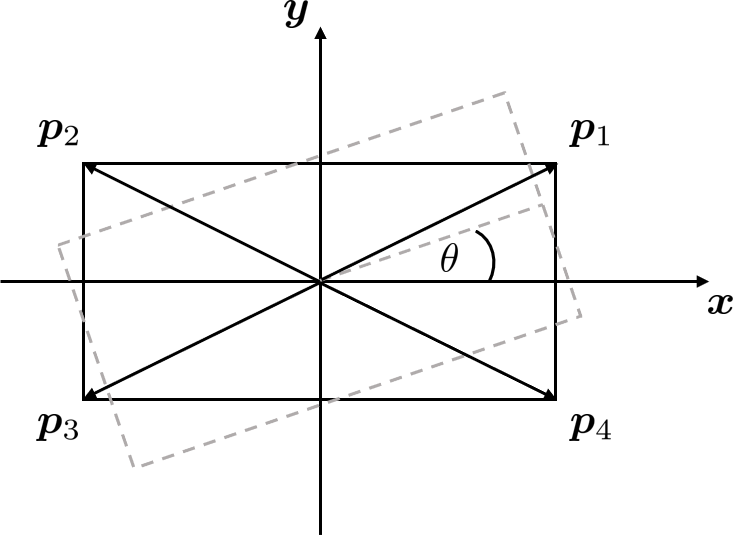
\includegraphics[scale=.5]{chapters/02_background/img/foot_convex_hull.png}
	\caption{The foot's support polygon, which is described by the position vectors $\bm{p}_i$.}
	\label{fig::212_foot_hull}
\end{figure}
A point $\bm{x}$ lies beneath the line that connects the edges if
\begin{align}
	\bm{A}^{L/R}\bm{x} \leq \bm{B}^{L/R},
	\label{eq::212_lin}
\end{align}
where the linear equations are defined by  $\bm{A}^{L/R}=\begin{pmatrix}
\bm{A}^{L/R,x}\,\bm{A}^{L/R,y}\end{pmatrix}\in\mathbb{R}^{N_{\text{edges}}\times2}$, and $\bm{B}^{L/R}\in\mathbb{R}^{N_{\text{edges}}\times1}$
\begin{align}
	\bm{A}^{L/R,x}[i] &= p^{L/R,y}_i-p^{L/R,y}_{i+1} \\
	\bm{A}^{L/R,y}[i] &= p^{L/R,x}_{i+1}-p^{L/R,x}_i \\
	\bm{B}^{L/R}[i] &= (p^{L/R,y}_i-p^{L/R,y}_{i+1})p^{L/R,x}_{i+1} + (p^{L/R,x}_{i+1}-p^{L/R,x}_i)p^{L/R,y}_{i+1}
\end{align}
Since we require the zero moment point to lie inside the support polygon, $\bm{x}$ in equation \ref{eq::212_lin} is replaced by $\bm{R}_z(f_k^\theta)(\bm{z}_k-\bm{f}_k)$, with $\bm{z}_k=\begin{pmatrix}
z_k^x & z_k^y
\end{pmatrix}^T$, and $\bm{f}_k=\begin{pmatrix}
f_k^x & f_k^y
\end{pmatrix}^T$. This expression describes the zero moment point with respect to the foot frame, where $\bm{R}_z(f_k^\theta) = \begin{pmatrix}
\quad\cos f_k^\theta & \sin f_k^\theta \\
-\sin f_k^\theta& \cos f_k^\theta
\end{pmatrix}$ is an inverse rotation around the z-axis that adds non-linearities to the constraints. We can now extend the formalism to the whole preview horizon by utilizing equations \ref{eq::212_zmp} and \ref{eq:312_feet}. This leads to (\href{https://github.com/mhubii/nmpc_pattern_generator/blob/5a213044c927dc6aac9f7e32ce1e5fb472cd67bb/libs/pattern_generator/src/base_generator.cpp#L946}{\underline{link}})
\begin{align}
	&\bm{D}_{k+1}(\bm{F}_{k+1}^{\theta})\begin{pmatrix}
		\bm{Z}_{k+1}^x - \bm{F}_{k+1}^x \\
		\bm{Z}_{k+1}^y - \bm{F}_{k+1}^y
	\end{pmatrix} \leq \bm{B}_{k+1} \\
	&\bm{D}_{k+1}(\bm{F}_{k+1}^{\theta})\begin{pmatrix}
		\bm{P}_{zs} \bm{c}_k^x + \bm{P}_{zu}\dddot{\bm{C}}_k^x - \bm{v}_{k+1}f_k^x-\bm{V}_{k+1}\tilde{\bm{F}}_{k+1}^x \\
		\bm{P}_{zs} \bm{c}_k^y + \bm{P}_{zu}\dddot{\bm{C}}_k^y - \bm{v}_{k+1}f_k^y-\bm{V}_{k+1}\tilde{\bm{F}}_{k+1}^y
	\end{pmatrix} \leq \bm{B}_{k+1}
	\label{eq::212_cop_hull}
\end{align}
where $\bm{D}_{k+1}\in\mathbb{R}^{N_\text{edges}N\times2N}$ depends on $\bm{F}_{k+1}^{\theta} = \bm{P}_{ps}f_k^\theta + \bm{P}_{pu}\bm{F}_{k+1}^\theta$, and holds all the linear equations on the whole preview horizon \begin{align}
\bm{D}_{k+1} = \begin{pmatrix}
	\bm{A}^{L/R,x}\bm{R}_z(f_{k+1}^\theta)&                  &\bm{0}                 &\bm{A}^{L/R,y}\bm{R}_z(f_{k+1}^\theta)&      &\bm{0} \\
	                  &\ddots            &                  &                  &\ddots& \\
	\bm{0}                 &                  &\bm{A}^{L/R,x}\bm{R}_z(f_{k+N}^\theta)&\bm{0}                 &      &\bm{A}^{L/R,y}\bm{R}_z(f_{k+N}^\theta)
\end{pmatrix},
\label{eq::212_rot1}
\end{align}
and $\bm{B}_{k+1}=\begin{pmatrix} \bm{B}^{L/R} & \dots & \bm{B}^{L/R}\end{pmatrix}^T$. Whether the left foot's or the right foot's convex hull is chosen depends on the support foot at the respective preview interval $k$. Equation \ref{eq::212_cop_hull} can now be expressed in terms of the free variables $\bm{U}_k$ by
\begin{align}
	\bm{D}_{k+1}\begin{pmatrix}
		\bm{P}_{zu} & -\bm{V}_{k+1} & \bm{0} & \bm{0}\\
		\bm{0} & \bm{0} & \bm{P}_{zu} & -\bm{V}_{k+1}
	\end{pmatrix}\bm{U}_k^{xy} &\leq \bm{B}_{k+1} + \bm{D}_{k+1}\begin{pmatrix}
		-\bm{P}_{zs}\bm{c}_k^x + \bm{v}_{k+1}f_k^x\\
		-\bm{P}_{zs}\bm{c}_k^y + \bm{v}_{k+1}f_k^y
	\end{pmatrix} \\
	\bm{A}_{\text{zmp},k}(\bm{U}_k^\theta)\bm{U}_k^{xy} &\leq \overline{\bm{U}_{\text{zmp},k}},
	\label{eq::212_ineq_zmp}
\end{align}
where $\overline{\bm{U}_{\text{zmp},k}}$ defines the upper bounds. The above derivation delivers a nice framework, which can be used to express the feasibility constraints as well.
\paragraph{Feasibility Constraints}
The feasibility constraints constrain the foot positioning to areas that the robot of interest can actually reach, which can again be defined as a set of linear inequalities, with the position vectors $\bm{p}_i$ that are shown in figure \ref{fig::212_foot_feasibility}. 
\begin{figure}[h!]
	\centering
	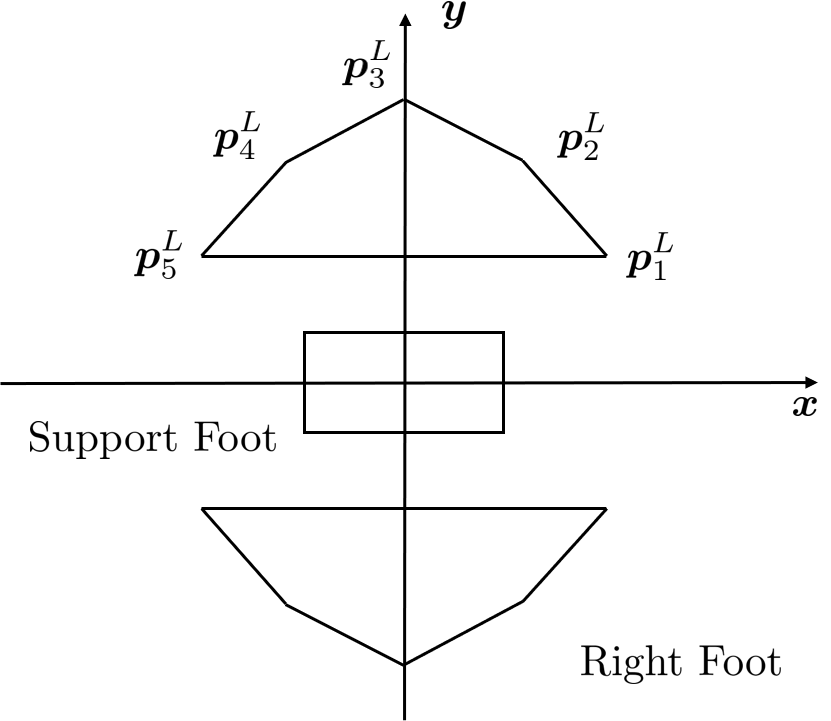
\includegraphics[scale=.5]{chapters/02_background/img/foot_constraints.png}
	\caption{The foot's feasibility polygon, which is described by the position vectors $\bm{p}_i$. The center is always defined by the current support foot's position, within the picture the support foot can therefore be the left as well as the right foot.}
	\label{fig::212_foot_feasibility}
\end{figure}
We can therefore just reuse the concept of equation \ref{eq::212_lin}, and replace $\bm{x}$ therein by the the difference of the next foot position $\tilde{\bm{F}}_{k}\in\mathcal{R}^{N_f\times1}$, and the previous one $\tilde{\bm{F}}_{k-1} = \bm{S}_0\tilde{\bm{F}}_{k} + \bm{S}_1f_k$, where $\bm{S}_0 = \begin{pmatrix}0 & 0 \\ \textbf{I}_{N_f-1} & 0
\end{pmatrix}\in\mathcal{R}^{N_f\times N_f}$ simply shifts $\tilde{\bm{F}}_{k}$ down by one row, and $\bm{S}_1 = \begin{pmatrix}
1 \\ 0 \\ \vdots \\ 0
\end{pmatrix}\in\mathcal{R}^{N_f\times1}$. Altogether we have (\href{https://github.com/mhubii/nmpc_pattern_generator/blob/dc1f5a9366cbbbf76f1b02cada642f6ac9a04c89/libs/pattern_generator/src/base_generator.cpp#L1061}{\underline{link}})
\begin{align}
\begin{pmatrix}
\bm{A}_{k+1}^{x}&\bm{A}_{k+1}^{y}\end{pmatrix} 
\begin{pmatrix}
\tilde{\bm{F}}^x_{k} - \bm{S}_0\tilde{\bm{F}}^x_{k} - \bm{S}_1f^x_k\\
\tilde{\bm{F}}^y_{k} - \bm{S}_0\tilde{\bm{F}}^y_{k} - \bm{S}_1f^y_k
\end{pmatrix} &\leq \bm{B}_{k+1} \\
\begin{pmatrix}
\bm{0} & \bm{A}_{k+1}^{x}(\textbf{I}_{N_f}-\bm{S}_0) & \bm{0} & \bm{A}_{k+1}^{y}(\textbf{I}_{N_f}-\bm{S}_0)
\end{pmatrix}\bm{U}_k^{xy} &\leq \bm{B}_{k+1}+\begin{pmatrix}
\bm{S}_1f_k^x \\ \bm{S}_1f_k^x 
\end{pmatrix}\\
\bm{A}_{\text{foot},k}(\bm{U}_k^\theta)\bm{U}_k^{xy} &\leq \overline{\bm{U}_{\text{foot},k}},
\label{eq::212_ineq_foot}
\end{align}
where $\bm{A}_{k+1}^{x/y}=\begin{pmatrix}
	\bm{A}^{L/R,x/y}\bm{R}_z(f_{k}^\theta)& & \bm{0} \\
	&\ddots &\\
	\bm{0} &           &\bm{A}^{R/L,x/y}\bm{R}_z(f_{k+N_fN}^\theta)
\end{pmatrix}\in\mathbb{R}^{N_\text{edges}N\times N_f}$ has alternating linear inequalities $\bm{A}^{L/R,x/y}\rightarrow\bm{A}^{R/L,x/y}$ that correspond on the support foot, and so does $\bm{B_{k+1}}\in\mathbb{R}^{N_\text{edges}N\times1}$. 
\paragraph{Relative Constraints}
By considering the maximum and minimum angle by which the feet are relatively oriented towards each other, we take hardware limits into account. Furthermore, the restriction of the maximally allowed relative angular velocity decreases that variation of acceleration before the foot landing \cite{naveau2016reactive}. The constraints can be formulated as follows (\href{https://github.com/mhubii/nmpc_pattern_generator/blob/dc1f5a9366cbbbf76f1b02cada642f6ac9a04c89/libs/pattern_generator/src/base_generator.cpp#L1244}{\underline{link}})
\begin{align}
	-\bm{\theta}_\text{max}\leq\bm{F}_{k+1}^{L,\theta} - \bm{F}_{k+1}^{R,\theta} &\leq \bm{\theta}_\text{max} \\
	-\dot{\bm{\theta}}_\text{max}\leq\dot{\bm{F}}_{k+1}^{L,\theta} - \dot{\bm{F}}_{k+1}^{R,\theta} &\leq \dot{\bm{\theta}}_\text{max},
\end{align}
which can be expressed in terms of the free variables with equations \ref{eq::212_ckp1} and \ref{eq::212_dckp1} to find
\begin{align}
	-\bm{\theta}_\text{max}-\bm{P}_{ps}(f_k^L-f_k^R)&\leq \begin{pmatrix}
	\bm{P}_{pu} & -\bm{P}_{pu}
	\end{pmatrix}\bm{U}_k^\theta \leq \bm{\theta}_\text{max}-\bm{P}_{ps}(f_k^L-f_k^R) \\
	\underline{\bm{U}_{\text{ori},k}}&\leq \bm{A}_{\text{ori},k}\bm{U}_k^\theta \leq \overline{\bm{U}_{\text{ori},k}}\\
		-\dot{\bm{\theta}}_\text{max}-\bm{P}_{vs}(f_k^L-f_k^R)&\leq \begin{pmatrix}
	\bm{P}_{vu} & -\bm{P}_{vu}
	\end{pmatrix}\bm{U}_k^\theta \leq \dot{\bm{\theta}}_\text{max}-\bm{P}_{vs}(f_k^L-f_k^R)\\
	\underline{\bm{U}_{\text{dori},k}}&\leq \bm{A}_{\text{dori},k}\bm{U}_k^\theta \leq \overline{\bm{U}_{\text{dori},k}}.
\end{align}
\paragraph{Obstacle Constraints}
In contrast to similar methods like \cite{herdt2010walking}, we also include the avoidance of convex obstacles by requesting that the feet's positions must lie outside of circles $C = \{(p^x, p^y)\in\mathbb{R}^2 \,|\, (p^x-x_0)^2+(p^y-y_0)^2\leq R^2\}$, which define the obstacles, where $x_0$, and $y_0$ define the obstacle's center in world coordinates. This can be formulated by the free variables by (\href{https://github.com/mhubii/nmpc_pattern_generator/blob/dc1f5a9366cbbbf76f1b02cada642f6ac9a04c89/libs/pattern_generator/src/base_generator.cpp#L1271}{\underline{link}})
\begin{align}
	&(f_k^x-x_0)^2 + (f_k^y-y_0)^2 \geq (R + m)^2
	\label{eq::212_obstacle}\\
	&\bm{U}_k^{xy,T}\begin{pmatrix}
	\bm{0} & \textbf{I}_{N_f} & \bm{0}& \textbf{I}_{N_f}
	\end{pmatrix}\bm{U}_k^{xy} - \\&\begin{pmatrix}
	\bm{0} & \begin{pmatrix}
	2x_0 & \dots & 2x_0
	\end{pmatrix} & \bm{0} & \begin{pmatrix}
	2y_0 & \dots & 2y_0
	\end{pmatrix}
	\end{pmatrix} \bm{U}_k^{xy}\geq \begin{pmatrix}
	(R + m)^2-x_0^2-y_0^2 \\
	\vdots \\
	(R + m)^2-x_0^2-y_0^2
	\end{pmatrix}\\
	&\bm{U}_k^{xy,T}\bm{H}_{\text{obs}}\bm{U}_k^{xy}+\bm{A}_{\text{obs}}\bm{U}_k^{xy} \geq \underline{\bm{U}_{\text{obs}}},
\end{align}
which expresses lower bounds for the free variables. Given the constraints, of which some are nonlinear, we can apply a Gauss-Newton method to find the optimal solution. This also implies that we have to linearize all of the constraints that were presented within the previous paragraphs. The linearization is described in the next paragraph - The Gauss-Newton Formulation.
\FloatBarrier
\subsubsection{The Gauss-Newton Formulation}
\label{sec::212_gn}
As outlined in equation \ref{eq::212_gn_min}, we can now linearize the quadratic problem of equation \ref{eq::212_canqp}. This leads to (\href{https://github.com/mhubii/nmpc_pattern_generator/blob/dc1f5a9366cbbbf76f1b02cada642f6ac9a04c89/libs/pattern_generator/src/nmpc_generator.cpp#L377}{\underline{link}})
\begin{align}
	\min_{\Delta\bm{U}_k}&\frac{1}{2}\Delta\bm{U}_k^T\bm{Q}_k\Delta\bm{U}_k + \tilde{\bm{p}}_k^T\Delta\bm{U}_k 
	\label{eq::212_ocp}\\
	\text{subject to: }&\underline{\tilde{\bm{U}}_k} \leq \tilde{\bm{A}}_k\Delta\bm{U}_k\leq\overline{\tilde{\bm{U}}_k},
\end{align}
where
\begin{align}
	&\tilde{\bm{p}}_k = \begin{pmatrix}
		\frac{1}{2}\bm{U}_{k-1}^{xy,T}\begin{pmatrix}
			\bm{Q}_k^x & \bm{0} \\
			\bm{0} & \bm{Q}_k^x
		\end{pmatrix} + \begin{pmatrix}
			\bm{p}_k^x \\ \bm{p}_k^y
		\end{pmatrix} \\
			\frac{1}{2}\bm{U}_{k-1}^{\theta,T}\begin{pmatrix}
			\bm{Q}_k^L & \bm{0} \\
			\bm{0} & \bm{Q}_k^R
		\end{pmatrix} + \begin{pmatrix}
			\bm{p}_k^L \\ \bm{p}_k^R
		\end{pmatrix} 
	\end{pmatrix} \\
	&\tilde{\bm{A}}_k = \begin{pmatrix}
		\bm{A}_{\text{zmp},k}(\bm{U}_{k-1}^\theta) & \nabla^T_{\bm{U}^\theta}\bm{A}_{\text{zmp},k}|_{\bm{U}_{k-1}^\theta}\bm{U}^{xy}_{k-1} \\
		\bm{A}_{\text{foot},k}(\bm{U}_{k-1}^\theta) & \nabla^T_{\bm{U}^\theta}\bm{A}_{\text{foot},k}|_{\bm{U}_{k-1}^\theta}\bm{U}^{xy}_{k-1} \\
		\bm{H}_\text{obs}\bm{U}^{xy}_{k-1}+\bm{A}_{\text{obs},k} & \bm{0} \\
		\bm{0} & \bm{A}_{\text{ori},k} \\
		\bm{0} & \bm{A}_{\text{dori},k}
	\end{pmatrix} \\
	&\underline{\tilde{\bm{U}}_k} = \begin{pmatrix}
		-\infty \\
		-\infty \\
		\underline{{\bm{U}}_\text{obs}}\\
		\underline{{\bm{U}}_\text{ori}}\\
		\underline{{\bm{U}}_\text{dori}}
	\end{pmatrix}-\bm{h}_{k-1},\,\overline{\tilde{\bm{U}}_k} = \begin{pmatrix}
		\overline{\bm{U}_{\text{zmp},k}}\\
		\overline{\bm{U}_{\text{foot},k}}\\
		\infty\\
		\overline{\bm{U}_{\text{ori},k}}\\
		\overline{\bm{U}_{\text{dori},k}}
	\end{pmatrix}-\bm{h}_{k-1}\\
	&\bm{h}_{k-1} =\begin{pmatrix}
		\bm{A}_{\text{zmp},k}(\bm{U}^\theta_{k-1})\bm{U}_{k-1}^{xy} \\
		\bm{A}_{\text{foot},k}(\bm{U}^\theta_{k-1})\bm{U}_{k-1}^{xy} \\
		\bm{U}_{k-1}^{xy,T}\bm{H}_{\text{obs}}\bm{U}_{k-1}^{xy}+\bm{A}_{\text{obs}}\bm{U}_{k-1}^{xy} \\
		\bm{A}_{\text{ori},k}\bm{U}_{k-1}^\theta\\
		\bm{A}_{\text{dori},k}\bm{U}_{k-1}^\theta
	\end{pmatrix}.
\end{align}
It follows that we only need to compute the gradient of $\bm{A}_{\text{zmp},k}$, and $\bm{A}_{\text{foot},k}$, with respect to the free variable $\bm{U}^{\theta}$, which can analytically be done by deriving the rotation matrices' gradient in equations \ref{eq::212_rot1}, and \ref{eq::212_ineq_foot}. The solution to this optimal control problem yields the update $\Delta\bm{U}_k$ to the current iterate $\bm{U}_k=\bm{U}_{k-1}+\Delta\bm{U}_k$ (\href{https://github.com/mhubii/nmpc_pattern_generator/blob/dc1f5a9366cbbbf76f1b02cada642f6ac9a04c89/libs/pattern_generator/src/nmpc_generator.cpp#L155}{\underline{link}}) under quadratic convergence, given that we are sufficiently close to a solution, as discussed earlier. The resulting positioning for the feet needs then to be interpolated, which will be explained in the following section - Interpolating Trajectories.  % nonlinear model predictive control
	\subsection{Interpolating Trajectories}
\label{sec::313_it}
As already shortly depicted in figure \ref{fig::31_pg}, we need to interpolate the trajectories that we obtain from the nonlinear model predictive control. This especially holds true for the feet, since the computed results do only consider the pendulums dynamic balance with respect to the x-, and the y-position, but not with respect to a robot that has to lift its feet along the z-axis. Furthermore, the feet's movement shall be executed such that they stop moving when they are about to touch the ground. This constraint, and others, will be achieved by interpolating the feet trajectories with polynomials. In order to then match the center of mass trajectory's temporal resolution with the feet trajectories', we will upscale it under the already well known assumption of a linear inverted pendulum. The resulting trajectories are shown in figure \ref{fig::313_ip}, and will further be explained in the following. 
\begin{figure}[h!]
	\centering
	\subcaptionbox{}%
	[.4\linewidth]{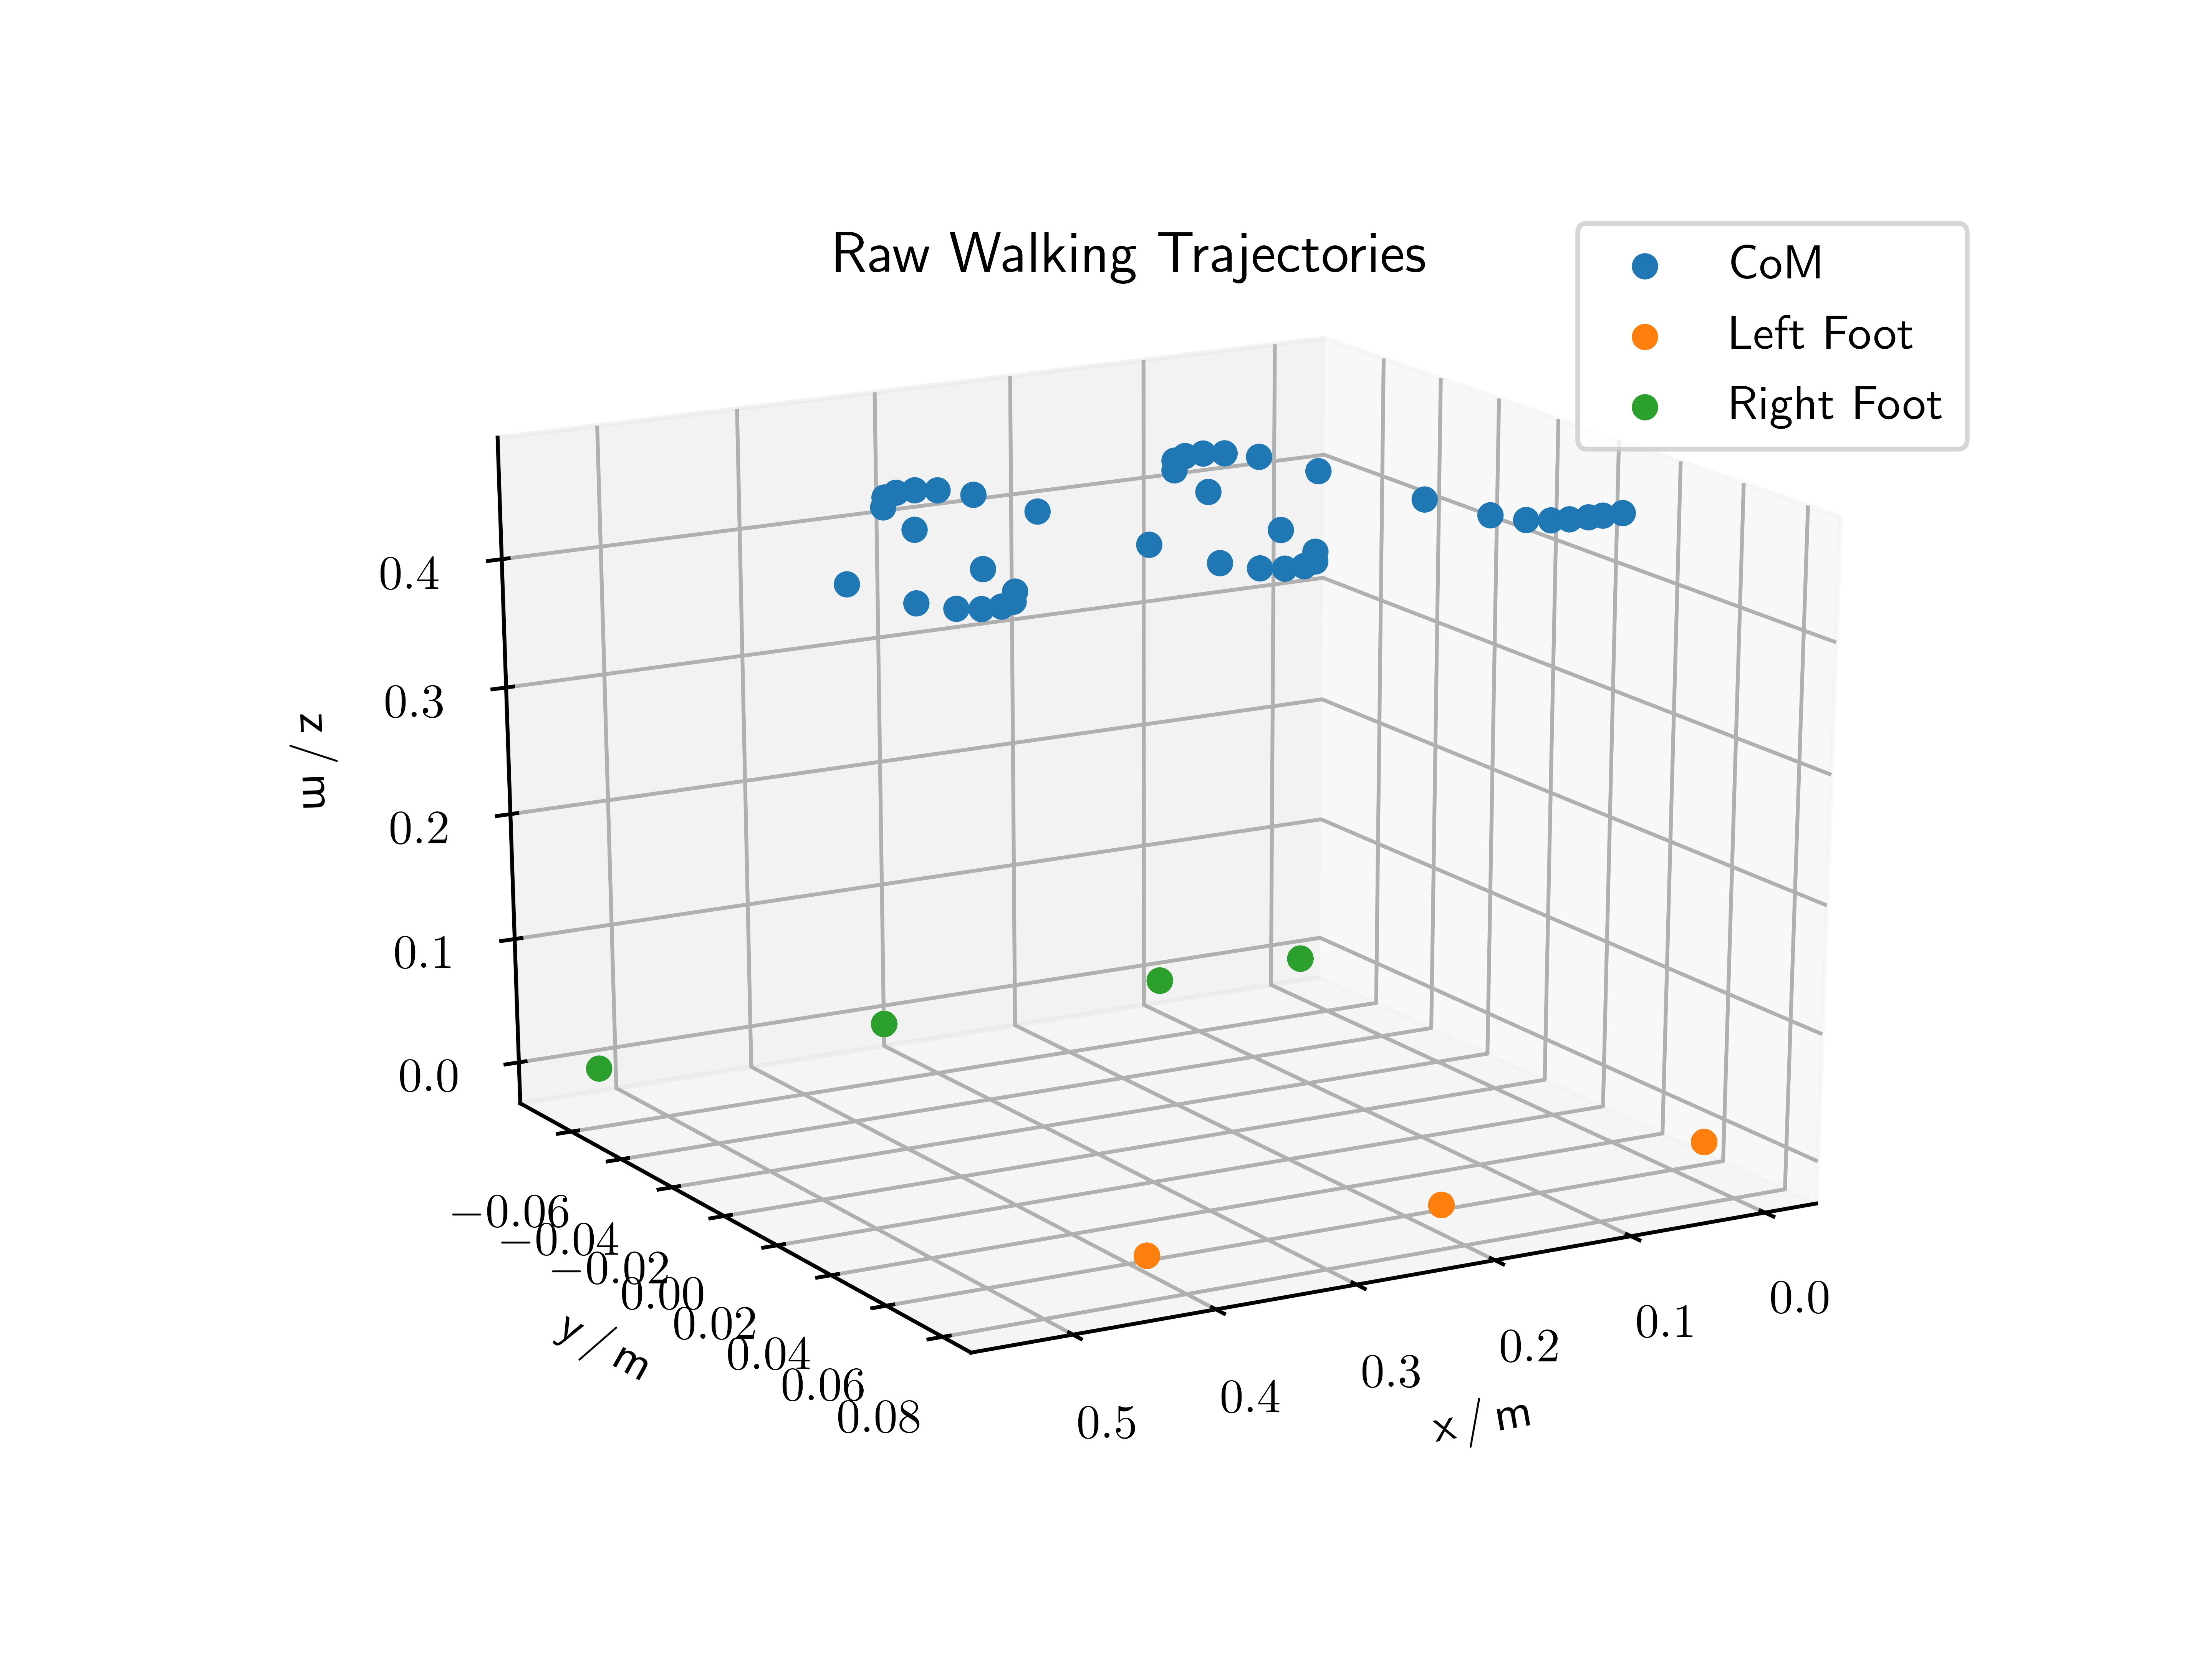
\includegraphics[scale=.4]{chapters/03_background/img/raw_results.png}}
	\subcaptionbox{}%
	[.4\linewidth]{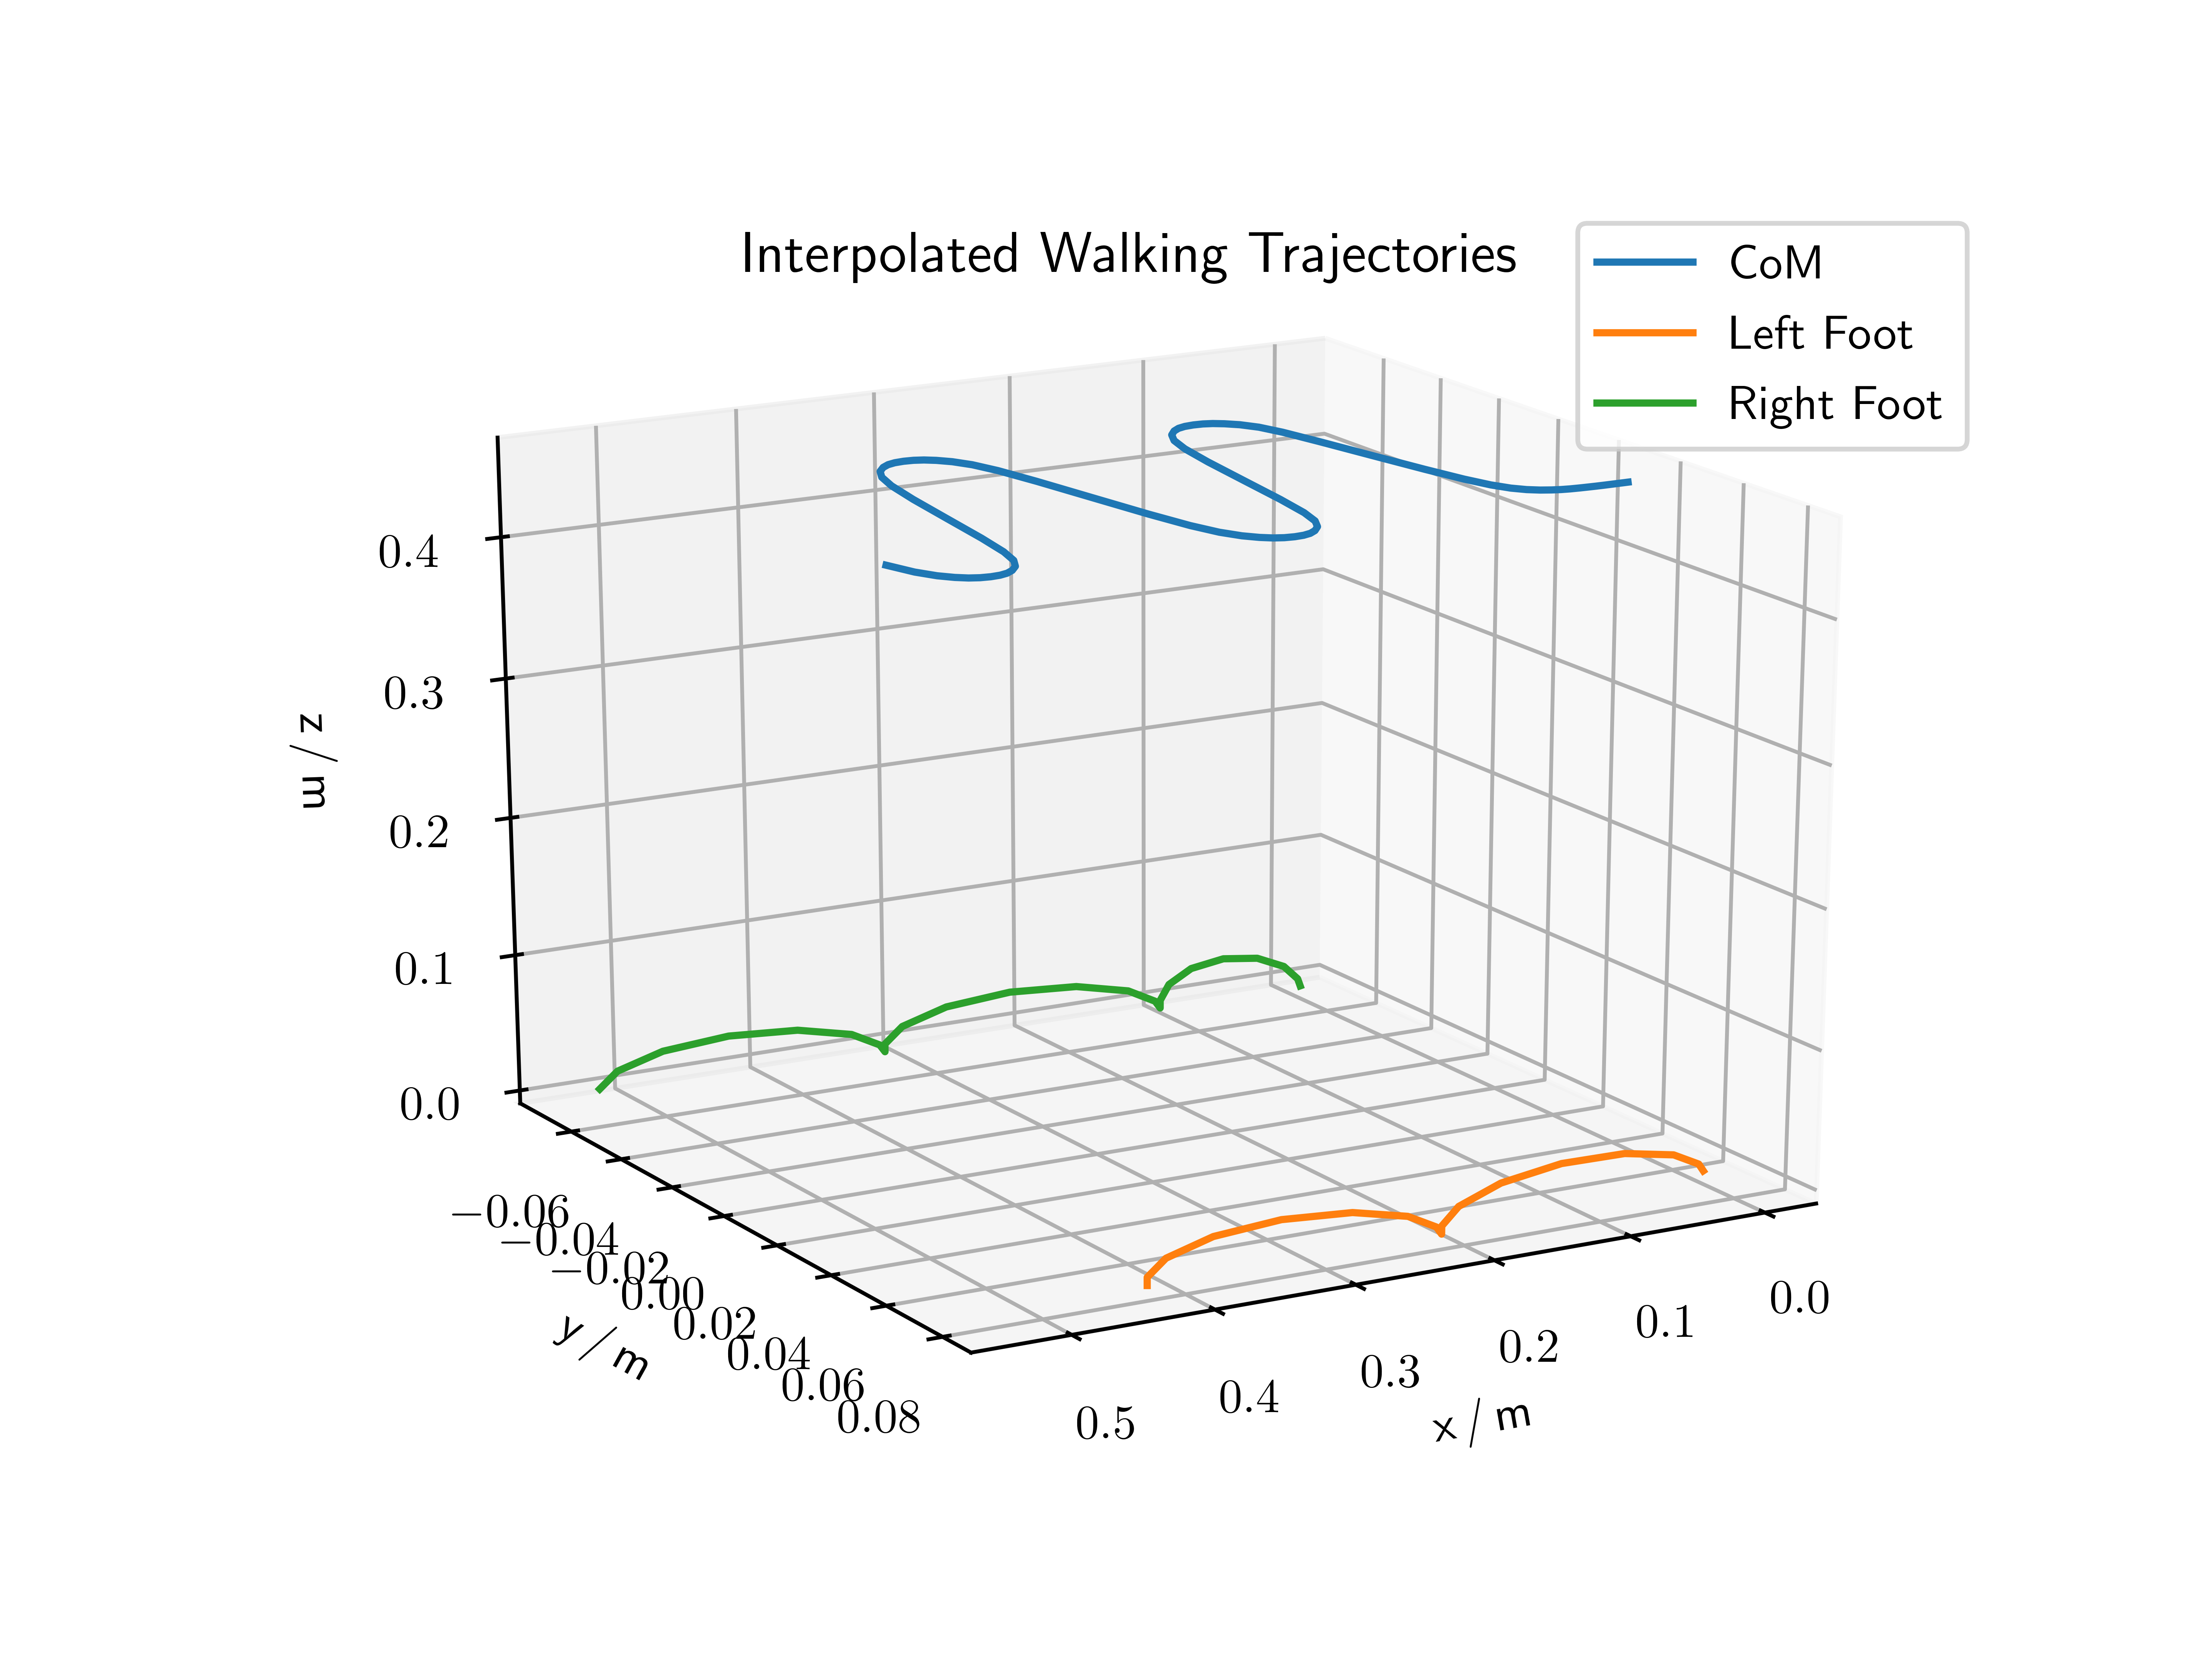
\includegraphics[scale=.4]{chapters/03_background/img/interpolated_results.png}}
	\caption{Uninterpolated trajectories (a), as obtained from the nonlinear model predictive control, and interpolated trajectories (b) for the feet and the center of mass.}
	\label{fig::313_ip}
\end{figure}
\subsubsection{Interpolating the Feet Trajectories}
Any trajectory can in principal be approximated by a polynomial function. For our purposes, we want to approximate positions $p$ as they evolve over time $t$, and further obtain the corresponding velocities $\dot{p}$ and accelerations $\ddot{p}$ (equations \ref{eq::313_pos_poly} - \ref{eq::313_acc_poly}).  
\begin{align}
	p(t) &= \sum_{i = 0}^{N}a_it^i 
	\label{eq::313_pos_poly}\\
	\dot{p}(t) &= \sum_{i = 1}^{N}ia_it^{(i-1)} 
	\label{eq::313_vel_poly}\\
	\ddot{p}(t) &= \sum_{i = 2}^{N}i(i-1)a_it^{(i-2)}
	\label{eq::313_acc_poly}
\end{align}
The coefficients $a_i$ of the polynomials can be chosen such that certain boundary conditions $\bm{b}$ are satisfied. For the lift-off and the drop-down of the robot's feet, these boundary conditions must satisfy a zero initial velocity $\dot{z}_\text{init}$ and a zero end velocity $\dot{z}_\text{end}$, as well as a zero initial height $z_\text{init}$ and a zero end height $z_\text{end}$, and a maximum step height $z_{T/2}$ in between, or else they will hit the ground in an unbalanced way. These conditions are listed below, where each height $z(t)$ and each velocity $\dot{z}(t)$ is written in terms of a polynomial, just as in equations \ref{eq::313_pos_poly} and \ref{eq::313_vel_poly}, respectively. 
\begin{align}
	z(t = 0) &= z_\text{init} = 0
	\label{eq::313_z_bound_1} \\
	\dot{z}(t = 0) &= \dot{z}_\text{init} = 0 \\
	z(t = \frac{T}{2}) &= z_{T/2}\\  
	z(t = T) &= z_\text{end} = 0 \\
	\dot{z}(t = T) &= \dot{z}_\text{end} = 0 
	\label{eq::313_z_bound_5}
\end{align}
To satisfy 5 boundary conditions, it is required to have a polynomial of 4th order with 5 coefficients $a_{z,i}$ in total. In matrix formulation we can express equations \ref{eq::313_z_bound_1} - \ref{eq::313_z_bound_5} as follows
\begin{align}
	\bm{M}_z\bm{a}_z &= \bm{b}_z \\
	\begin{pmatrix}
		1 & 0 & 0              & 0              & 0 \\
		0 & 1 & 0              & 0              & 0 \\
		1 & \left(\frac{T}{2}\right)        & \left(\frac{T}{2}\right)^2  & \left(\frac{T}{2}\right)^3 & \left(\frac{T}{2}\right)^4 \\
		1 & T & T^2            & T^3            & T^4 \\
		0 & 1 & 2T             & 3T^2           & 4T^3 
	\end{pmatrix}
	\begin{pmatrix}
		a_{z,0} \\
		a_{z,1} \\
		a_{z,2} \\
		a_{z,3} \\
		a_{z,4}
	\end{pmatrix} &=
	\begin{pmatrix}
		z_\text{init} \\
		\dot{z}_\text{init} \\
		z_{T/2} \\
		z_\text{end}\\
		\dot{z}_\text{end}
	\end{pmatrix}.
\end{align}
Inversion then yields
\begin{align}
	\bm{a}_z&=\bm{M}_z^{-1}\bm{b}_z \\
	\begin{pmatrix}
		a_{z,0} \\
		a_{z,1} \\
		a_{z,2} \\
		a_{z,3} \\
		a_{z,4}
	\end{pmatrix} &=
	\begin{pmatrix}
		1 & 0 & 0 & 0 & 0 \\
		0 & 1 & 0 & 0 & 0 \\
		-\frac{11}{T^2} & -\frac{4}{T} & \frac{16}{T^2} & -\frac{5}{T^2} & \frac{1}{T} \\
		\frac{18}{T^3} & \frac{5}{T^2} & -\frac{32}{T^3} & \frac{14}{T^3} & -\frac{3}{T^2} \\
		-\frac{8}{T^4} & -\frac{2}{T^3} & \frac{16}{T^4} & -\frac{8}{T^4} & \frac{2}{T^3}
	\end{pmatrix}
	\begin{pmatrix}
		z_\text{init} \\
		\dot{z}_\text{init} \\
		z_{T/2} \\
		z_\text{end}\\
		\dot{z}_\text{end}
	\end{pmatrix}.
\end{align}
The obtained coefficients $a_i$ are then used to compute the height of each foot during a single support phase (\href{https://github.com/mhubii/nmpc_pattern_generator/blob/c82c64a28da7527e75442764f585bd50a8f61ee9/libs/pattern_generator/src/interpolation.cpp#L779}{\underline{link}}). The maximum step height $z_{T/2}$ (\href{https://github.com/mhubii/nmpc_pattern_generator/blob/c82c64a28da7527e75442764f585bd50a8f61ee9/libs/pattern_generator/configs.yaml#L22}{\underline{link}}), and the single support time $T$ (\href{https://github.com/mhubii/nmpc_pattern_generator/blob/c82c64a28da7527e75442764f585bd50a8f61ee9/libs/pattern_generator/configs.yaml#L21}{\underline{link}}), which is the step time minus the double support time, can be set in the configurations file. For the x-, and the y-positions of the feet, we can define boundary conditions in a similar fashion. In contrary to the computation of the z-position, the x-, and the y-position interpolation of the feet allows for feedback. Therefore, we require additional constraints that satisfy the accelerations as follows
\begin{align}
	x(t = 0) &= x_\text{init} 
	\label{eq::313_x_bound_1}\\
	\dot{x}(t=0) &= \dot{x}_\text{init} \\
	\ddot{x}(t=0) &= \ddot{x}_\text{init} \\
	x(t=T) &= x_\text{end}\\
	\dot{x}(t=T) &= \dot{x}_\text{end} \\
	\ddot{x}(t=T) &= \ddot{x}_\text{end}.
	\label{eq::313_x_bound_6}
\end{align}
Again, we can rewrite equations \ref{eq::313_x_bound_1} - \ref{eq::313_x_bound_6} in matrix formulation
\begin{align}
	\bm{M}_x\bm{a}_x &= \bm{b}_x \\
	\begin{pmatrix}
		1 & 0 & 0 & 0 & 0 & 0 \\
		0 & 1 & 0 & 0 & 0 & 0 \\
		0 & 0 & 2 & 0 & 0 & 0 \\
		1 & T & T^2 & T^3 & T^4 & T^5 \\
		0 & 1 & 2 T & 3 T^2 & 4 T^3 & 5 T^4 \\
		0 & 0 & 2 & 6 T & 12 T^2 & 20 T^3
	\end{pmatrix}
	\begin{pmatrix}
		a_{x,0} \\
		a_{x,1} \\
		a_{x,2} \\
		a_{x,3} \\
		a_{x,4} \\
		a_{x,5}
	\end{pmatrix} &=
	\begin{pmatrix}
		x_\text{init} \\
		\dot{x}_\text{init} \\
		\ddot{x}_\text{init} \\
		x_\text{end} \\
		\dot{x}_\text{end} \\
		\ddot{x}_\text{end} 
	\end{pmatrix},
\end{align}
and inversion yields the polynomial's coefficients $a_{x,i}$
\begin{align}
	\bm{a}_x &= \bm{M}_x^{-1}\bm{b}_x \\
	\begin{pmatrix}
		a_{x,0} \\
		a_{x,1} \\
		a_{x,2} \\
		a_{x,3} \\
		a_{x,4} \\
		a_{x,5}
	\end{pmatrix} &= 
	\frac{1}{2}
	\begin{pmatrix}
		2 & 0 & 0 & 0 & 0 & 0 \\
		0 & 2 & 0 & 0 & 0 & 0 \\
		0 & 0 & 1 & 0 & 0 & 0 \\
		-\frac{20}{T^3} & -\frac{12}{T^2} & -\frac{3}{T} & \frac{20}{T^3} & -\frac{8}{T^2} & \frac{1}{T} \\
		\frac{30}{T^4} & \frac{16}{T^3} & \frac{3}{T^2} & -\frac{30}{T^4} & \frac{14}{T^3} & -\frac{2}{T^2} \\
		-\frac{12}{T^5} & -\frac{6}{T^4} & -\frac{1}{T^3} & \frac{12}{T^5} & -\frac{6}{T^4} & \frac{1}{T^3} \\
	\end{pmatrix}
	\begin{pmatrix}
		x_\text{init} \\
		\dot{x}_\text{init} \\
		\ddot{x}_\text{init} \\
		x_\text{end} \\
		\dot{x}_\text{end} \\
		\ddot{x}_\text{end} 
	\end{pmatrix}.
\end{align}
The exact same formalism is used to interpolate the foot's y-position during single support phase (\href{https://github.com/mhubii/nmpc_pattern_generator/blob/c82c64a28da7527e75442764f585bd50a8f61ee9/libs/pattern_generator/src/interpolation.cpp#L806}{\underline{link}}). In contrast to the interpolation of the feet's positions, the center of mass positions will be extrapolated under the introduced assumption of a linear inverted pendulum. The method will be shortly explained in the following paragraph - Interpolating the Center of Mass Trajectories.
\subsubsection{Interpolating the Center of Mass Trajectories}
The center of mass trajectories can now simply be adjusted to the temporal resolution of the feet trajectories by applying the linear time stepping scheme from equation \ref{eq::312_ltss} with an adjusted temporal resolution $T$. An iterative application (\href{https://github.com/mhubii/nmpc_pattern_generator/blob/5a213044c927dc6aac9f7e32ce1e5fb472cd67bb/libs/pattern_generator/src/interpolation.cpp#L776}{\underline{link}}) of these matrices then yields the desired interpolation. The only requirement left to get our robot to walk is now the transformation of trajectories in Cartesian space to trajectories within the joint space, which will be resolved in the following chapter - Kinematics.   % interpolation
	\FloatBarrier
\subsection{Kinematics}
\label{sec::214_k}
As already shortly depicted in figure \ref{fig::21_pg}, it is required to compute the robot's kinematics in order to switch between the Cartesian space and the joint space. For our purposes we need to find joint angles that satisfy the center of mass and the feet trajectories. While it is rather straight forward to compute the forward kinematics, as it is just a concatenation of spatial transformations, the inverse kinematics require an optimization, since there usually is no unique solution.
\FloatBarrier
\subsubsection{Forward Kinematics}
\label{sec::2141_fk}
The goal in forward kinematics is to transform joint angles $\bm{q}$ into Cartesian coordinates $\bm{x}$ such that $\textbf{FK}(\bm{q}) = \bm{x}$. For this thesis, it enables us to feedback the robot's center of mass position, given the current state of it. In terms of homogeneous coordinates, one can express the forward kinematics as a series of spatial transformations, which include translations $\bm{t}$ and rotations $\bm{R}$ 
\begin{align}
	\bm{x}_\text{0} = \prod_{i=N}^{0}\bm{H}_i^{i-1}(q)\bm{x}_\text{N},
\end{align}
where $\bm{x}_i=[x\,y\,z\,1]^T$, and $\bm{H}_i^{i-1}=\begin{pmatrix}\bm{R} & \bm{t} \\ \bm{0} & 1 \end{pmatrix}$ are homogeneous coordinates and transformations from frame $i$ to frame $i-1$, respectively.
\FloatBarrier
\subsubsection{Inverse Kinematics}
\label{sec::2142_ik}
In inverse kinematics, we aim at finding joint angles $\bm{q}$ that satisfy certain positional and orientational constraints, which we set for the kinematic chain of interest. For this work, we require the robot's feet and center of mass to be at a position that we obtain from the nonlinear model predictive control. That is, we minimize the sum of squared differences $S(\bm{q},\Delta\bm{q})$ between desired positions and orientations $a_i$ and the linearization of the forward kinematics around the robot's current pose $\bm{q}$ (equation \ref{eq::2142_min}), to find an incremental update $\Delta\bm{q}$. 
\begin{align}
	S(\bm{q},\Delta\bm{q}) = \sum_{i=0}^m\left[a_i-\textbf{FK}_i(\bm{q})-\frac{\partial\textbf{FK}_i(\bm{q})}{\partial\bm{q}}\Delta\bm{q}\right]^2
	\label{eq::2142_min}
\end{align}
A damped version of this minimization yields the Levenberg-Marquardt algorithm \cite{more1978levenberg}\cite{sugihara2011solvability}, with which one can iteratively update the pose $\bm{q}$ by $\Delta\bm{q}$, so to satisfy the posed requirements (equation \ref{eq::2142_levenberg}).
\begin{align}
	\Delta\bm{q} = (\bm{J}^T\bm{J}+\lambda\bm{I})^{-1}\bm{J}^T(\bm{y}-\textbf{FK}(\bm{q}))
	\label{eq::2142_levenberg}
\end{align}
Therein, the rows of system's Jacobian $\bm{J}$ is governed by $\bm{J}_i=\frac{\partial\textbf{FK}_i(\bm{q})}{\partial\bm{q}}$.   % kinematics
	
	\FloatBarrier
\section{Machine Learning}  
\label{sec::22_ml}
Machine learning methods do play a major role for autonomous navigation of robots, and whilst most recent approaches mainly dealt with tree search methods in 3D point-clouds, we aim at utilizing neural networks for solving the task at hand, since it enables us to combine spatial, semantic, and temporal understanding into one approach. Within this chapter, we will, therefore, explain the required fundamentals on neural networks in section \ref{sec::221_nn}, then cover two possible methods for training a neural network, one of which is supervised \ref{sec::222_bc}, whereas the second method bases on reinforcement learning \ref{sec::223_rl}, and finally explain image processing techniques in section \ref{sec::224_ip}, which allow us to extract depth maps from stereo images, so to help the neural networks understand the seen content. The goal here clearly is to introduce a method that is biologically inspired, in that it works directly in the image domain, which is very similar to how humans observe their environment. Therefore, we will shortly explain the biological similarities to a human brain within the next section - Neural Networks.   % short overview of machine learning
	\subsection{Neural Networks}
\label{sec::321_nn}
Neural networks are inspired by the brain's structure, and as we will see later in this chapter, their building blocks can be thought of as neurons (figure \ref{fig::321_neuron}).
\begin{figure}[h!]
	\centering
	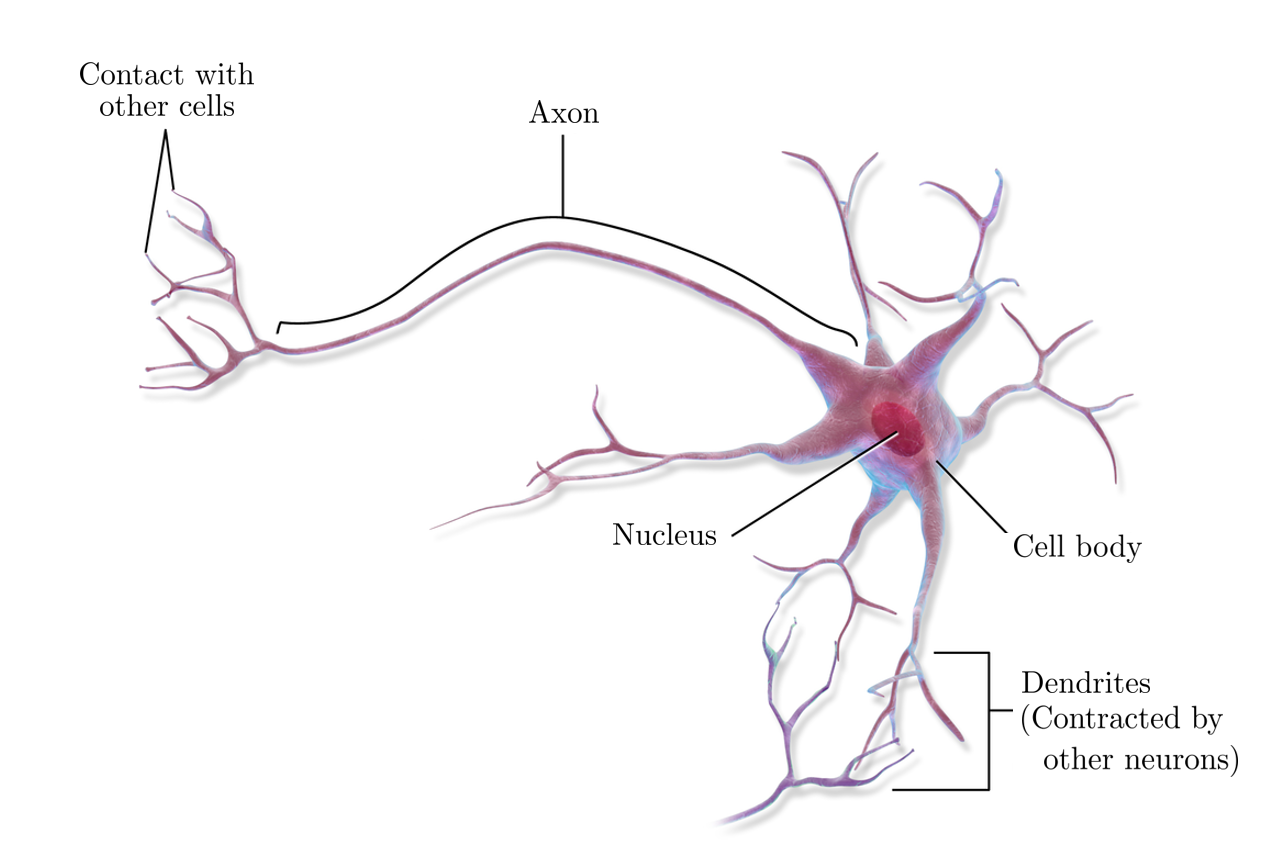
\includegraphics[scale=.35]{chapters/03_background/img/neuron.png}
	\caption{Biological neuron, which connects its cell body to dendrites of surrounding neurons via an axon. \cite{haggstrom2014medical}}
	\label{fig::321_neuron}
\end{figure}
And although neural networks have gained early attention in research, they have only recently become powerful for their implementation on graphic processing units (GPUs) \cite{oh2004gpu}. This was caused by their mathematical description that is linear and can be parallalized very well. Running neural nets on GPUs on the other hand consumes a lot of energy, which stays in contrast to biological neurons, which communicate by brief energy efficient spikes \cite{hodgkin1952quantitative}. And while there are around 100 billion neurons in the human brain, currently huge neural networks have around a factor of 10000 less \cite{goodfellow2016deep}. Not only is the number of neurons in a neural net comparably small, but also is their complexity way below that of a biological neuron. To tackle this discrepancy, and to learn complicated tasks, it is therefore required to introduce activation functions for neural networks, such as the rectifying linear unit \cite{krizhevsky2012imagenet}. This enables neural networks to be used on a variety of problems, but they currently lack in transferring knowledge between different domains, and tend to over-fit certain tasks. There exist methods to deal with this tendency, such as max-pooling \cite{weng1992cresceptron} or dropout \cite{srivastava2014dropout} layers, which efficiently just reduce the number of neurons within a neural net. To build a good understanding of neural networks, we will introduce different architectures in the following that will be used throughout this thesis, and we will start with the simplest in the next paragraph - Fully Connected Neural Network.
\subsubsection{Fully Connected Neural Network}
The biologically inspired perceptron model \cite{viglione19704} lay the foundation for neural networks and it got extended pretty soon to the multi-layer perceptron model
\cite{ivakhnenko1971polynomial}, which is known today as the fully connected neural network. Due to its similarity to the brain's structure, it is often depicted as in figure \ref{fig::321_fully_connected}, where each orange circle represents a neuron that is connected to its surroundings via simple weights $w_{ij}$, as neurons inside the brain are by synapses.
\begin{figure}[h!]
	\centering
	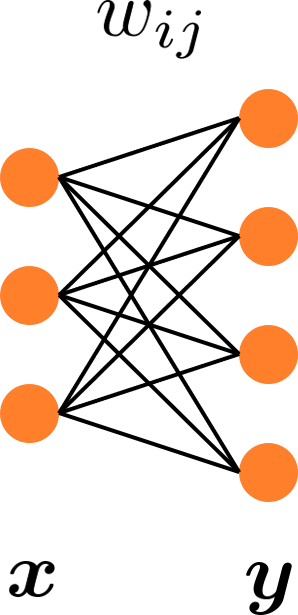
\includegraphics[scale=.28]{chapters/03_background/img/fully_connected.png}
	\caption{Fully connected neural network with three inputs and four outputs. Each orange circle represents what is often referred to as neuron, while the black lines indicate the connections between each neuron.}
	\label{fig::321_fully_connected}
\end{figure}
Mathematically speaking, the feed forward process can be described as a simple matrix multiplication with all weights $\bm{W}$, where the input $\bm{x}$ gets converted to the output $\bm{y}$ via
\begin{align}
	\bm{y} = \bm{W}\bm{x}+\bm{b}
	\label{eq::321_fully_connected}
\end{align}
Therein, the bias $\bm{b}$ can be understood as a shift of isolines that are introduced by hyperplanes. These hyperplanes are learned and expressed by the layer's weights $w_{ij}$ (figure \ref{fig::321_classification}). The output $\bm{y}$, is then further passed through an activation function $f$, and therefore can be compared to the action potential inside a neuron, as it determines the amount by which the next neuron gets excited. This activation function can be anything from a simple step function for classification to a linear function for regression. In practice there are some activation functions that have shown to be of particular use and we will introduce them later in this chapter.
\begin{figure}[h!]
	\centering
	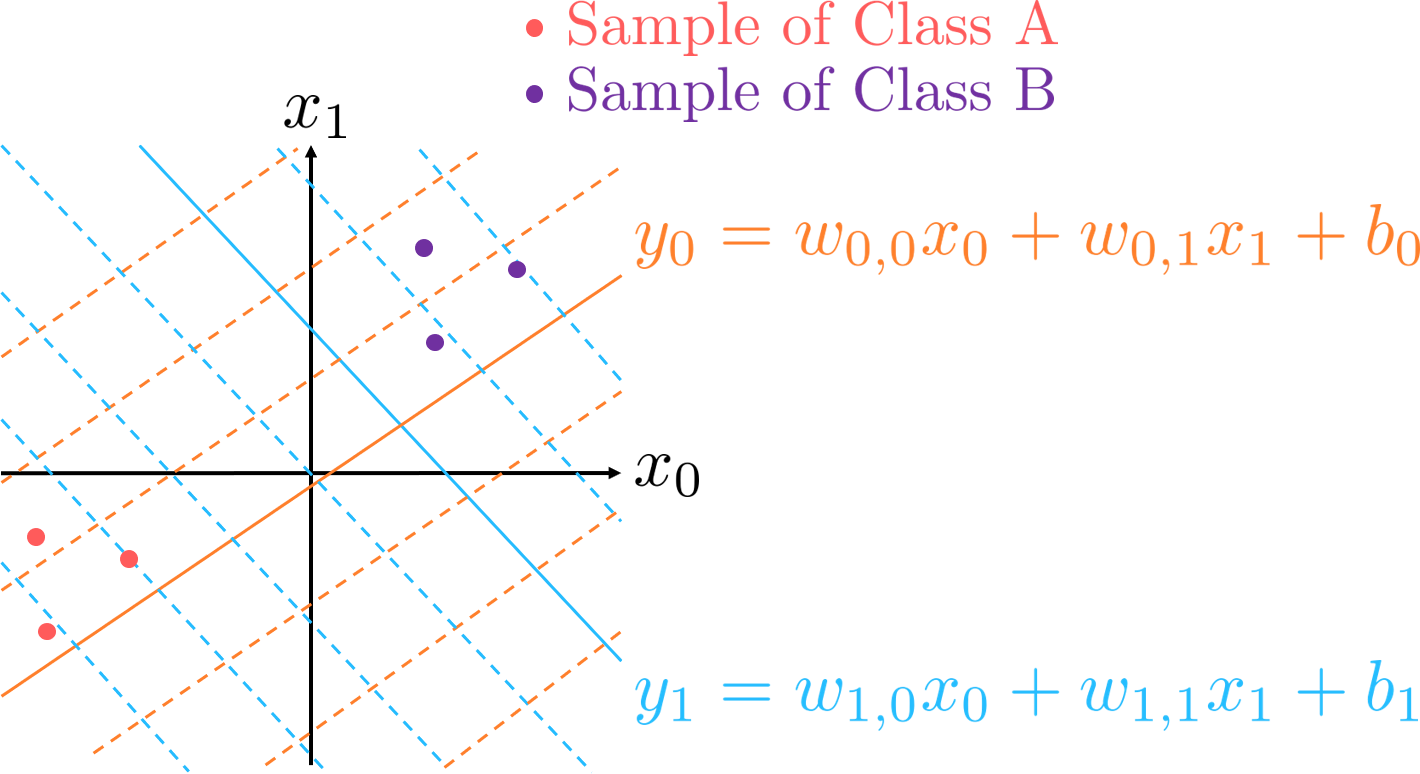
\includegraphics[scale=.28]{chapters/03_background/img/classification.png}
	\caption{Simple interpretation of a fully connected neural network with one layer that takes $\bm{x}=(x_0\,\,x_1)^T$ as input. The dotted lines are isolines to the hyperplane, which showcase the effect of the bias $\bm{b}$.}
	\label{fig::321_classification}
\end{figure}
\subsubsection{Convolutional Neural Network}
The concept of convolutional neural networks was first inspired by biological structures inside the visual cortex of the human brain. It was introduced as neocognitron \cite{fukushima1980neocognitron}, and soon after termed convolutional neural network for its mathematical properties, in that it equals convolutions. Figure \ref{fig::321_convolutional} shows how an input $\bm{x}$ is fed forward through the network architecture across two layers.   
\begin{figure}[h!]
	\centering
	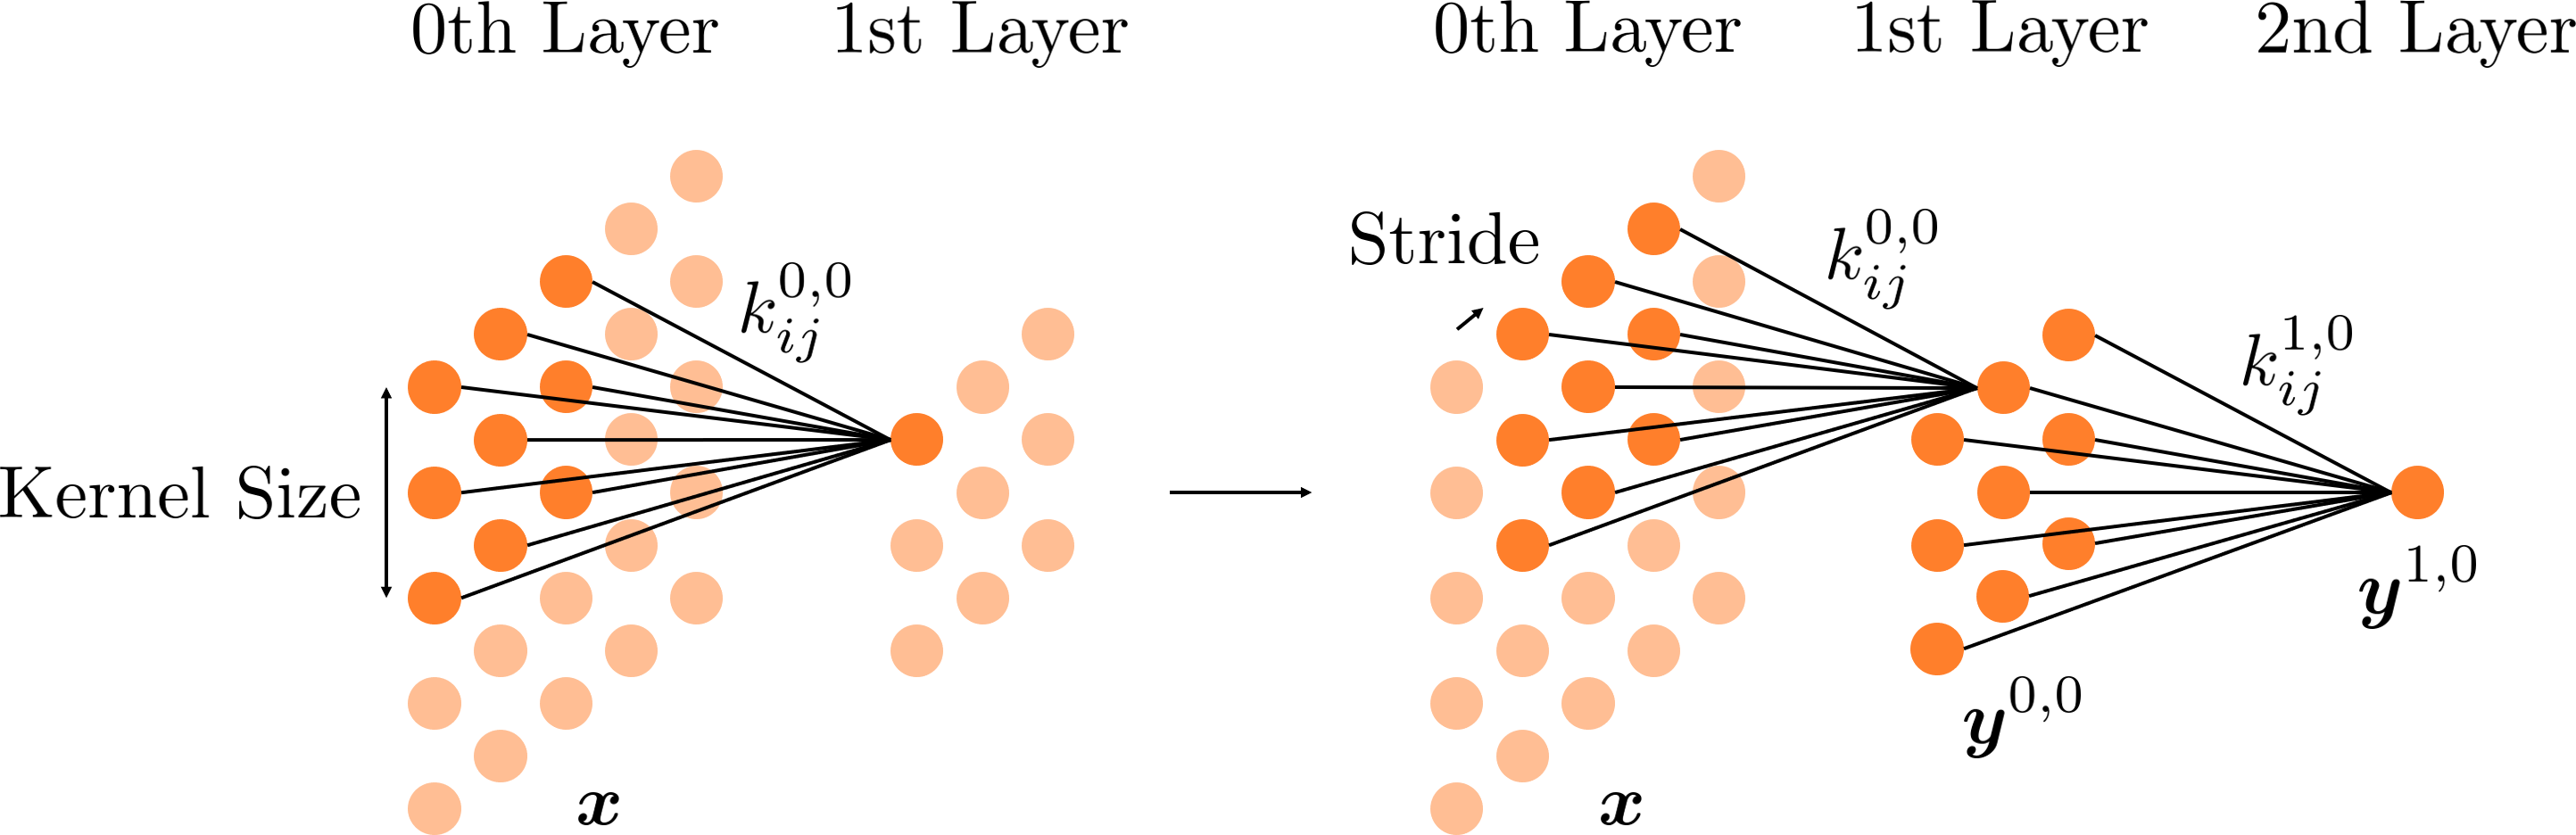
\includegraphics[scale=.28]{chapters/03_background/img/convolutional.png}
	\caption{Convolutional neural network with a total of three layers of which one is the input layer. For visualization, the kernel size is set to be three, and the stride is set to be one.}
	\label{fig::321_convolutional}
\end{figure}
The operation is again visualized by utilizing orange circles, which may be referred to as neurons. These neurons are connected by weights $k^{l,n}_{ij}$, which together constitute the kernel $\bm{k}^{l,n}$ of each convolution. Therein, $l$ stands for the current layer, and $n$ indexes the kernel within a layer, as there may in principle be many different kernels for a single layer. Mathematically speaking, we can formulate the process as follows
\begin{align}
	\bm{y}^{0,0} &= f(\bm{x}*\bm{k}^{0,0}) \\
	\bm{y}^{1,0} &= f(\bm{y}^{0,0}*\bm{k}^{1,0})	
\end{align}
One thing to notice is that the deeper we go, meaning the more layers we have, the more of the initial input contributes to the current activation. This can be seen in figure \ref{fig::321_convolutional}, where each neuron within the first layer only sees a kernel size sized snipped of the original input $\bm{x}$, whereas a neuron within the second layer already sees all of it. This intuitive understanding of convolutional neural networks is backed by visualizations of the highest activity neuron's gradient with respect to the input, where the gradient itself equals the transposed convolution \cite{simonyan2013deep}.  Figure \ref{fig::321_transposed_conv} shows transposed convolutions for a classification network that was trained on ImageNet \cite{deng2009imagenet}. It can be seen that while superficial layers learn to understand edges, deeper layers grab more complex spatial correlations within images, such as car wheels within the third layer.
\begin{figure}[h!]
	\centering
	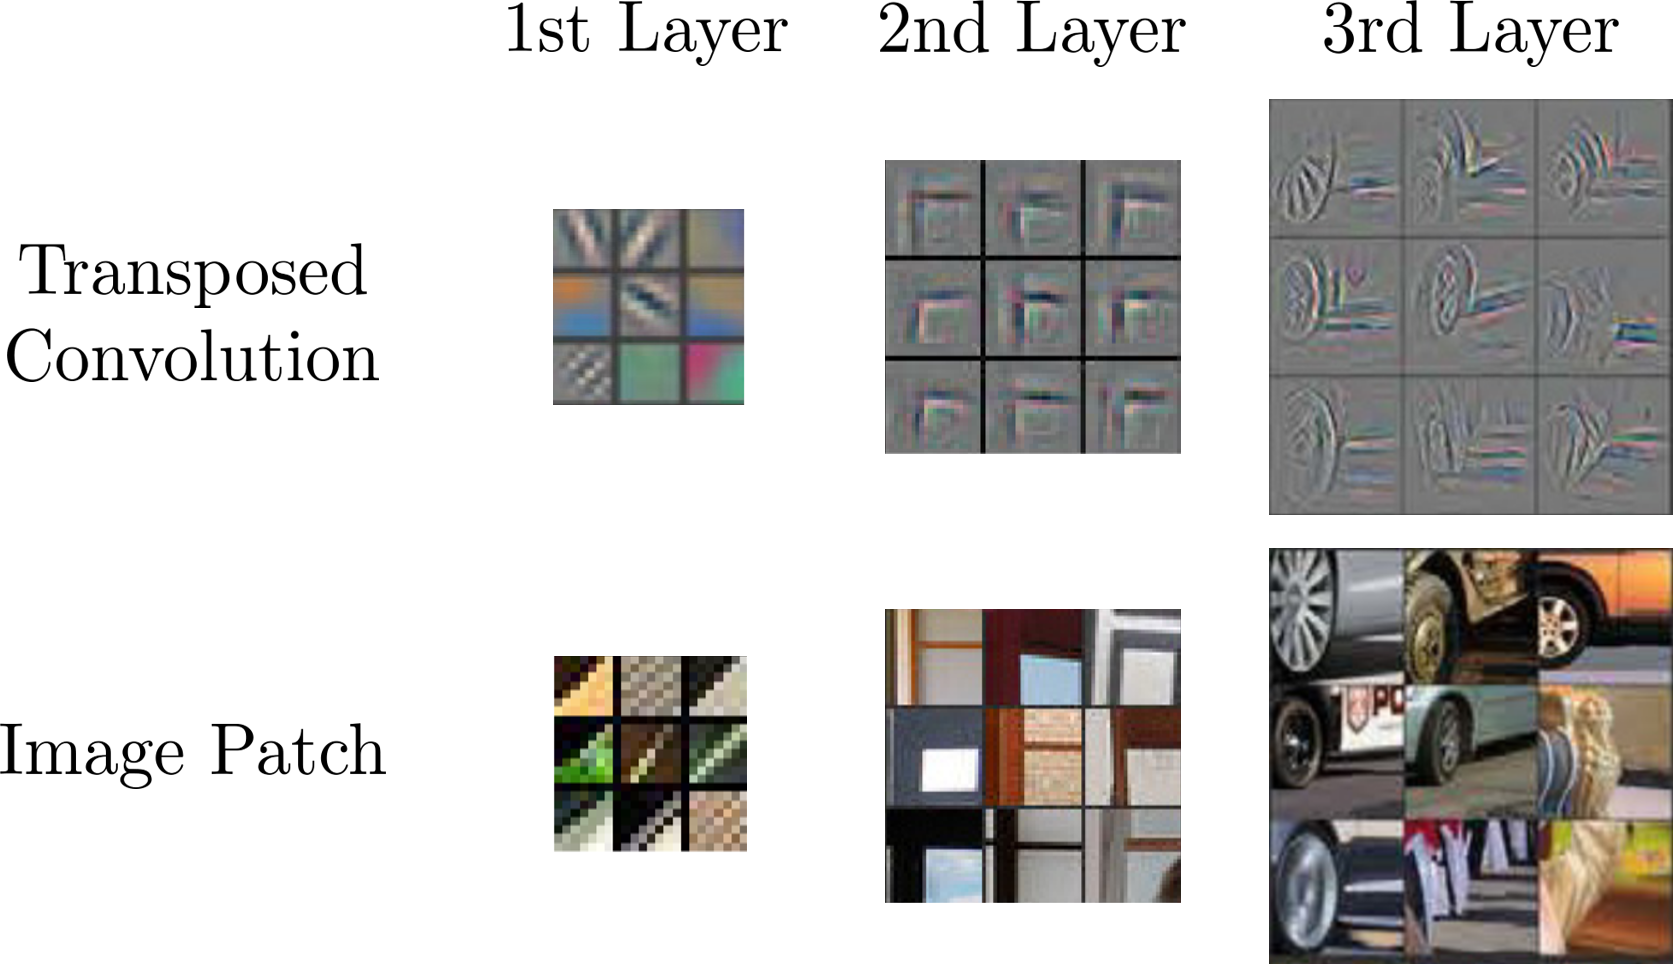
\includegraphics[scale=.28]{chapters/03_background/img/transposed_conv.png}
	\caption{Analysis of neurons with highest activation, corresponding to a subset of ImageNet. For the first layer, the kernel itself is shown, and image patches at the kernel's scale. For the second and third layer, a single neuron with highest activation is upscaled by transposed convolutions to the first layer's feature map. Images taken from \cite{zeiler2014visualizing}.}
	\label{fig::321_transposed_conv}
\end{figure}
Therefore, convolutional neural networks are particularly well suited for understanding spatial correlations, and while recent advancements also propose the promising use of convoltional neural networks for time series analysis \cite{vaswani2017attention}, a simpler approach are long short-term memory units, which will be explained in the next section - Long Short-Term Memory. 
\subsubsection{Long Short-Term Memory}
Long short-term memory units were introduced to overcome the vanishing and exploding gradient problem for recurrent neural networks in time series analysis \cite{hochreiter1997long}. That is the gradient tends to diverge exponentially over the course of the backward pass towards earlier inputs, resulting in intractable updates for the weights of the neural network. This issue got solved by adding a constant recurrent self-connection that allows for constant error propagation through the network, which got further refined by replacing the constant self-connection with a forget gate \cite{gers1999learning}. The inner workings of a long short-term memory unit is shown in figure \ref{fig::321_lstm}. 
\begin{figure}[h!]
	\centering
	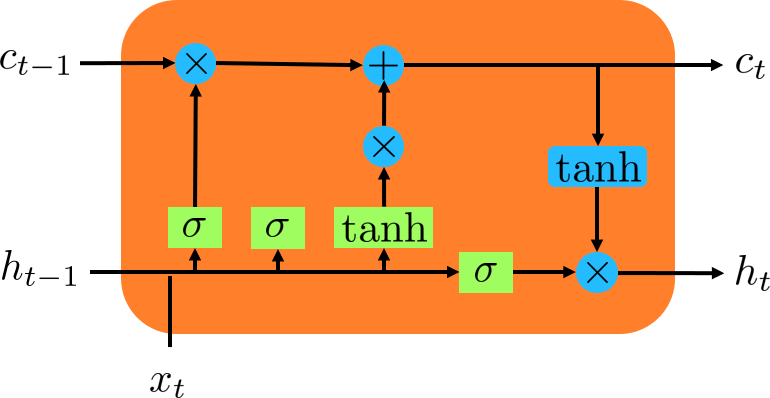
\includegraphics[scale=.28]{chapters/03_background/img/lstm.png}
	\caption{Long short-term memory unit with cell states $\bm{c}_i$, hidden states $\bm{h}_i$, input $\bm{x}_t$, and activation functions $\sigma/\tanh$, as well as addition $+$ and multiplication $\times$ operators.}
	\label{fig::321_lstm}
\end{figure}
The underlying mathematical operations can therein be expressed as follows
\begin{align}
	\bm{i}_t &= \sigma(\bm{W}_{ii}\bm{x}_t+\bm{b}_{ii}+\bm{W}_{hi}\bm{h}_{t-1}+\bm{b}_{hi})\\
	\bm{f}_t &= \sigma(\bm{W}_{if}\bm{x}_t+\bm{b}_{if}+\bm{W}_{hf}\bm{h}_{t-1}+\bm{b}_{hf})\\
	\bm{g}_t &= \tanh(\bm{W}_{ig}\bm{x}_t+\bm{b}_{ig}+\bm{W}_{hg}\bm{h}_{t-1}+\bm{b}_{hg})\\
	\bm{o}_t &= \sigma(\bm{W}_{io}\bm{x}_t+\bm{b}_{io}+\bm{W}_{ho}\bm{h}_{t-1}+\bm{b}_{ho})\\
	\bm{c}_t &= \bm{f}_t\cdot c_{t-1} + \bm{i}_t\cdot\bm{g}_t\\
	\bm{h}_t &= \bm{o}_t \cdot\tanh(\bm{c}_t),
\end{align}
where $\cdot$ is an element-wise multiplication. The sigmoid function $\sigma$, which ranges from 0 to 1, assures that the input gate $\bm{i}_t$, the forget gate $\bm{f}_t$, and the output gate $\bm{o}_t$ let only pass values of interest into, and out of the cell. Multiple long short-term memory units can then be linked for time series analysis as shown in figure \ref{fig::321_lstm_chain}.
\begin{figure}[h!]
	\centering
	
\includegraphics[scale=.28]{chapters/03_background/img/lstm_chain.png}
	\caption{Chain of long short-term memory units for temporal understanding of the input sequence $\bm{x}_i$.}
	\label{fig::321_lstm_chain}
\end{figure}
\subsubsection{Backpropagation}
The currently most popular way to train a neural network is backpropagation, which got first introduced in \cite{linnainmaa1970representation}. It has no biological equivalent but poses an effective way to optimize a huge amount of parameters. Newer methods use evolutionary algorithms and treat network parameters as population that develops over time \cite{montana1989training}, but we wont consider them further. The reason for why backpropagation works so well to optimize neural networks, is the simplicity of the mathematical operations that make them up. Not only do the activation functions have an analytical derivative, but further can we just apply the chain rule multiple times on the loss function, so to find the gradient for every network parameter. Suppose we have the loss $L$, then the derivative with respect to the weights $\bm{W}_l$ of layer $l$, is just given as
\begin{align}
	\frac{\partial L}{\partial \bm{W}_l} = \bm{\delta}_l\bm{x}_{l-1}^T,
	\label{eq::321_bp}
\end{align}
where for the last layer $N$, and all previous layers $l$, we have
\begin{align}
	\bm{\delta}_N &= \frac{\partial L}{\partial \bm{x}_N} \cdot f_N'(\bm{W}_N\bm{x}_{N-1}) \\
	\bm{\delta}_l &= \bm{W}^T_{l+1}\bm{\delta}_{l+1} \cdot f_{l}'(\bm{W}_l\bm{x}_{l-1}),
\end{align} % https://sudeepraja.github.io/Neural/
with $f'$ being the derivative of the corresponding activation function. The update for the next time-step $t+1$ is then performed according to an optimizer specific learning rate $\bm{\alpha}_{\bm{W}^t_l}$ as follows
\begin{align}
	\bm{W}_l^{t+1} = \bm{W}_l^t - \bm{\alpha}_{\bm{W}^t_l}\cdot\frac{\partial L}{\partial \bm{W}^l},
\end{align}
where $\cdot$ is an element-wise multiplication.   % short introduction to neural networks
	\FloatBarrier
\subsection{Behavioral Cloning}
\label{sec::222_bc}
Behavioral cloning in itself is not always related to machine learning, but poses one possible way of training a neural net in a supervised manner. The presented concept is easy to understand and got inspired by \cite{bojarski2016end}, where it was used for self-driving cars, and since having a car drive along the road is easier to achieve than having a robot walk around an environment, we will deal with the additional details later to focus on the main points for now. The proposed method utilizes the control loop, which was already introduced in figure \ref{fig::2_cl}. In order to then replace the human user by an artificial agent, we have a human user perform a desired behavior, and copy it. The required extended control loop is shown in figure \ref{fig::222_bc}.
\begin{figure}[h!]
	\centering
	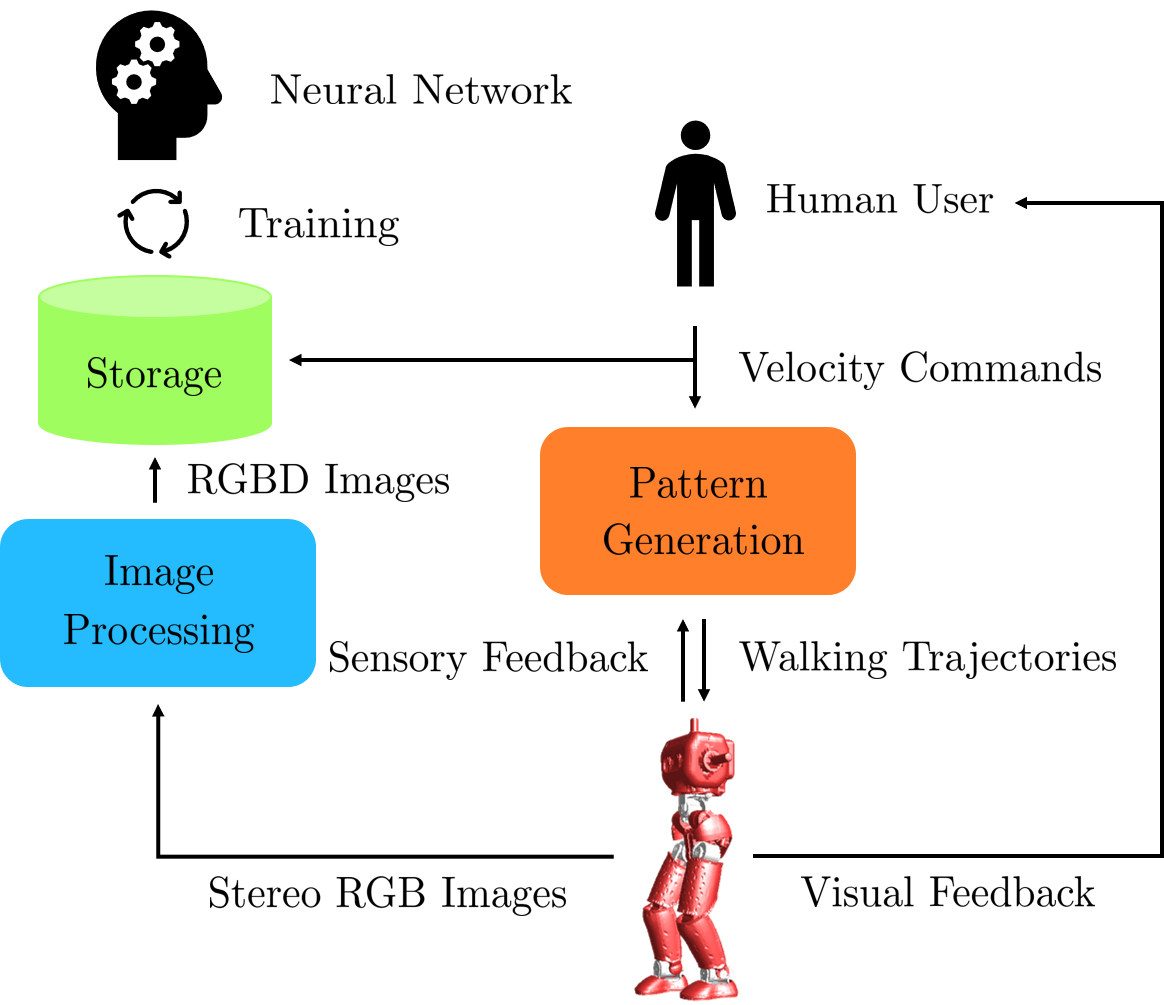
\includegraphics[scale=.5]{chapters/02_background/img/behavioral_cloning.png}
	\caption{Pipeline for behavioral cloning. The neural network is trained on stored RGBD images, and corresponding velocity commands that are correlated by a timestamp}
	\label{fig::222_bc}
\end{figure}
It simply takes the velocity commands from the human user, and stores it alongside RGBD images with a corresponding timestamp to some storage, where the RGBD images are obtained from stereo RGB images by an image processing step that is explained in section \ref{sec::224_ip}. The timestamp allows to correlate seen images to desired velocities afterwards, which in turn enables an artificial agent to train on the stored data. For our purposes, the artificial agent is a neural network. An appropriately chosen network architecture will then enable us to learn the taught behavior and ultimately lets us replace the human user. This procedure relies on prior knowledge to achieve certain tasks, namely the stored data. It is therefore extremely import to assure that the sampled data, from which we want to learn a task, does not introduce any unwanted bias, that is, we need to take care of the distribution from which we sample in the first place. In principle, it is possible to learn any arbitrary behavior with this technique, but this requires not only good data, but also a vast amount of it. There are other algorithms that explore the state space on their own, and for which we could for example use the taught behavior as prior as well. These algorithms belong to the class of reinforcement learning methods, and we will have a look at a particular one in the next section.   % behavioral cloning
	\FloatBarrier
\subsection{Reinforcement Learning}
\label{sec::223_rl}
The goal in reinforcement learning is not only to learn actions $a_t$ at time-step $t$, given a state $s_t$, like it is in behavioral cloning, but further to explore actions and states. This is usually performed as shown in figure \ref{fig::223_rl}, where an agent interacts with an environment to receive a reward $r_t$, and also changes the state as cause of its action. Therein, the actions $a_t$ are sampled from a policy $a_t\sim\pi_\theta(a_t|s_t)$ that depends on parameters $\theta$, which for our case are simply the weights of a neural network. 
\begin{figure}[h!]
	\centering
	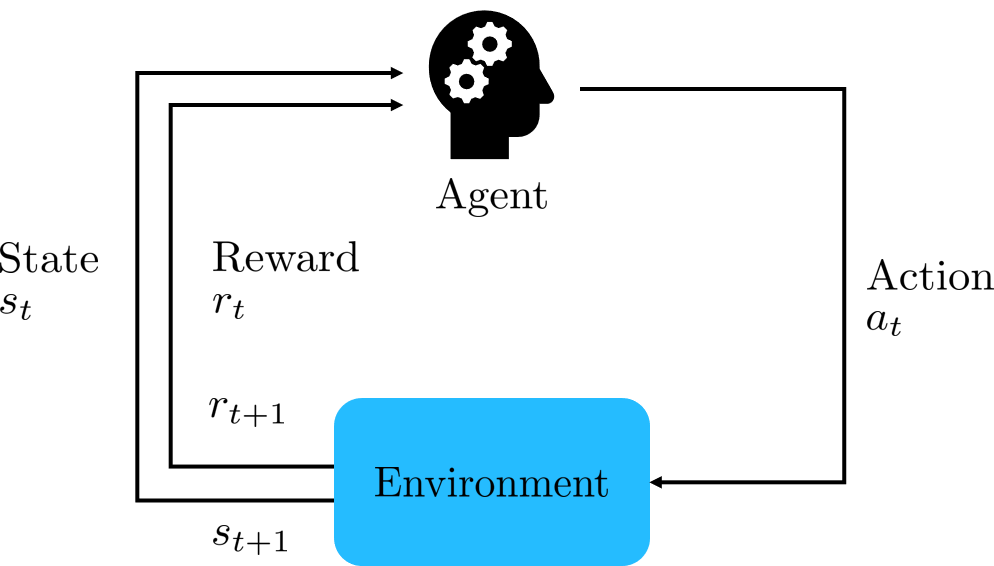
\includegraphics[scale=.5]{chapters/02_background/img/reinforcement_learning.png}
	\caption{Reinforcement learning setup. As the agent interacts with the environment, the state of the environment changes.}
	\label{fig::223_rl}
\end{figure}
The difficulty in optimizing the policy $\pi_\theta$, is to have an agent to discard immediate rewards over future expected rewards. For discrete action spaces, this got well solved by deep Q-learning \cite{mnih2015human}. Different approaches for continuous action spaces like trust region policy optimization \cite{schulman2015trust} are rather complicated. The, to this date, most elegant way of solving continuous control problems in a reinforcement learning setup, is proximal policy optimization \cite{schulman2017proximal}, and we will elaborate on it in the following. Gradient policy methods, such as proximal policy optimization, try to update the policy $\pi_\theta$, such that the expected total future reward $\mathbb{E}\left[\sum_{t=0}^\infty r_t\right]$ is maximized. For the incremental update, it is therefore required to find the gradient of this expression
\begin{align}
	\nabla_\theta\mathbb{E}_{a_t\sim\pi_\theta}\left[\sum_{t=0}^\infty r_t\right] = \mathbb{E}_{a_t\sim\pi_\theta}\left[\sum_{t=0}^\infty\psi_t\nabla_\theta\log\pi_\theta(a_t|s_t)\right],
\end{align}
where $\psi_t$ can take many forms. Since the gradient is just an estimate, as it is computed from samples being taken from the reinforcement learning environment, it usually suffers from variance and bias. As shown in \cite{schulman2015high}, we can trade-off variance for bias and the other way around, by replacing $\psi_t$ for the general advantage estimate $\hat{A}^\text{GAE}_t$ as follows
\begin{align}
	\hat{A}^{\text{GAE}(\gamma,\lambda)}_t = \sum_{l=0}^\infty(\gamma\lambda)^l\delta_{t+l}^V,
	\label{eq::223_gae}
\end{align}
where $\delta^V_{t,l} = r_t + \gamma V(s_{t+1}) - V(s_t)$ is the temporal difference \cite{sutton1998introduction}, and $V$ the value function, which is given by a critic network. The critic's goal then is to have the gradient estimate steer the acting policy network towards actions that maximize the reward. A huge problem therein is that the policy may diverge and that policies may be discarded on the basis of a gradient estimate with a high variance. This is prohibited in proximal policy optimization by clipping the general advantage estimate, and therefore the gradient, under the following objective
\begin{align}
	L^\text{CLIP} = \min(\rho_t(\theta)\hat{A}_t, \text{clip}(\rho_t(\theta), 1-\epsilon, 1+\epsilon)\hat{A}_t),
	\label{eq::223_clip}
\end{align}
where $\rho_t(\theta) = \frac{\pi_\theta(a_t|s_t)}{\pi_{\theta_\text{old}}(a_t|s_t)}$ is the probability ratio of the old and the new policy. The loss is shown in figure \ref{fig::223_ppo}, and it assures for a positive advantage estimate that the gradient does not diverge towards actions that are way more likely under the new policy, than they have been for the old policy.
\begin{figure}[h!]
	\centering
	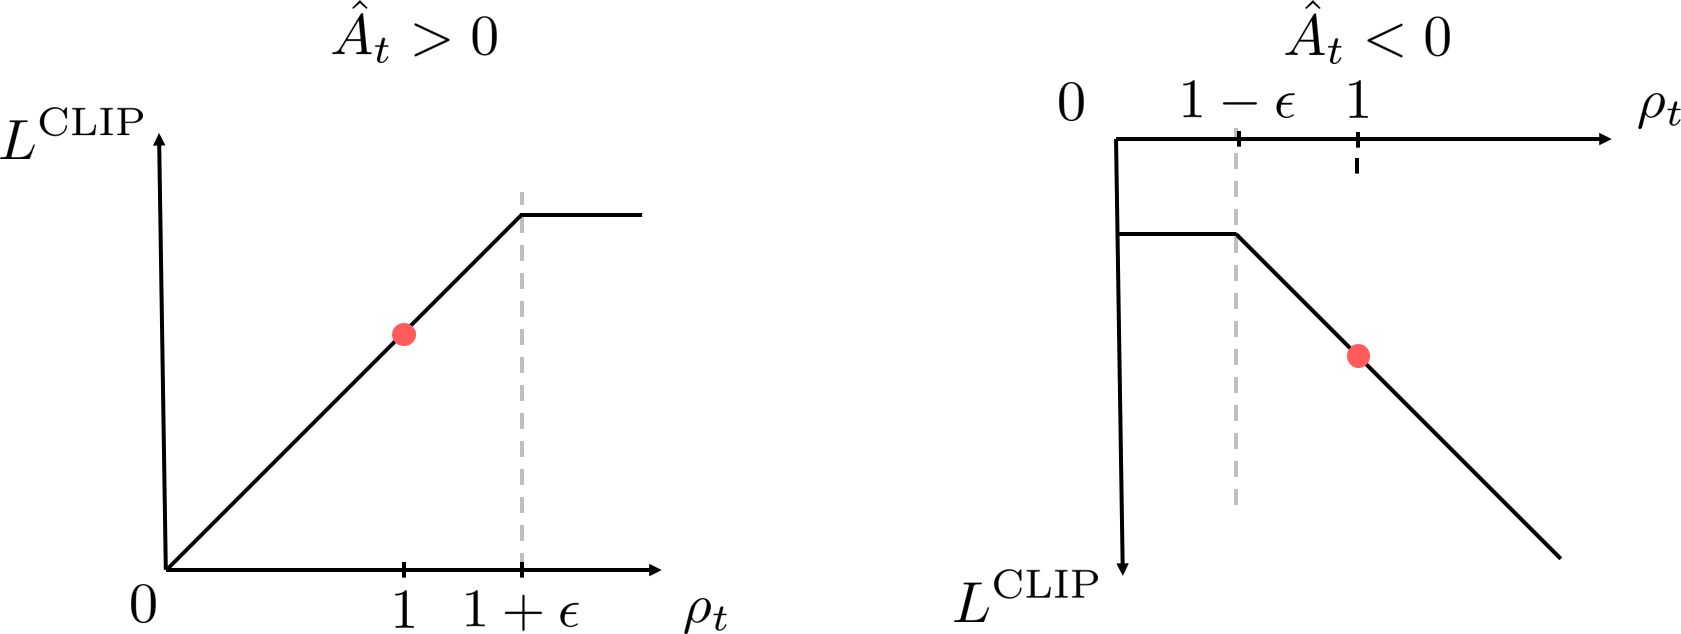
\includegraphics[scale=.35]{chapters/02_background/img/ppo_objective.png}
	\caption{Policy gradient clipping in proximal policy optimization for positive and negative advantage estimates $\hat{A}_t$.}
	\label{fig::223_ppo}
\end{figure}
Also, for a negative advantage estimate, it assures that the gradient points aways from these policies. The total objective $L_t^{\text{CLIP}+\text{VF}+\text{S}}$ of proximal policy optimization is further extended by an entropy term $S$ that results in exploration, and the critic's loss $L^\text{VF}$, such that it can steer the gradient (equation \ref{eq::223_ppo_loss}).
\begin{align}
	L_t^{\text{CLIP}+\text{VF}+\text{S}} = \mathbb{E}\left[L_t^\text{CLIP}(\theta)-c_1L_t^\text{VF}(\theta)+c_2S\left[\pi_\theta\right](s_t)\right]
	\label{eq::223_ppo_loss}
\end{align}
The critic's loss therein is the squared-error of the value function estimate and the explored values $(V_\theta(s_t)-V^\text{target}_t)^2$. The algorithm then runs as follows
\begin{algorithm}
	\SetAlgoLined
	\For{iteration = 1,2,...}{
		\For{runs=1,2,...}{
			Run policy $\pi_{\theta_\text{old}}$ in environment for $T$ timesteps\\
			Compute advantage estimates $\hat{A}^\text{GAE}_1$,...,$\hat{A}^\text{GAE}_T$
		}
		Optimize surrogate $L$ wrt $\theta$, with $K$ epochs and minibatch size $M\leq NT$\\
		$\theta_\text{old}\leftarrow\theta$
	}
	\caption{PPO, Actor-Critic Style}
	\label{alg::225_ac}
\end{algorithm}   % reinforcement learning
	\FloatBarrier
\subsection{Image Processing}
\label{sec::224_ip}
In the previous sections, we have learned about two different approaches to train neural nets on solving certain tasks. Although we came to understand that the complexity of the task to be solved correlates strongly with the amount of data at hand, there exist domains from which it is undeniably easier to do so. To equip a neural network with some prior knowledge by switching the domain may therefore not only be highly desirable but sometimes also needed if the amount or quality of data is not sufficient. One domain which is of special interest when it comes to interacting in a three-dimensional environment is a domain that represents depth information. If there are any, it may sometimes be possible to extract this kind of prior knowledge from a depth camera. As for this work, we need to rely on stereo cameras and powerful algorithms that allow us to compute depth images in real-time. The algorithm that helps us to do so, in terms of the extraction of weighted least squares disparity maps \cite{min2014fast}, will be presented in the following paragraph - Depth Map Extraction.
\FloatBarrier
\subsubsection{Depth Map Extraction}
As already pointed out, the depth map is generated from stereo camera images by a technique called stereo block matching \cite{hamzah2010sum}. This method works best for edge filtered images, as will become clear soon. To obtain edge filtered images $\bm{E}$, the stereo RGB images are first converted into grayscale $\bm{G}$, which are then convolved with the Sobel kernel $\bm{S}_x$ along the horizontal axis \cite{sobel2014an} (equation \ref{eq::224_sobel_conv}, figure \ref{fig::224_image_preprocessing}). 
\begin{align}
	\bm{E} = \bm{S}_x*\bm{G}
	\label{eq::224_sobel_conv}
\end{align}
\begin{figure}[h!]
	\centering
	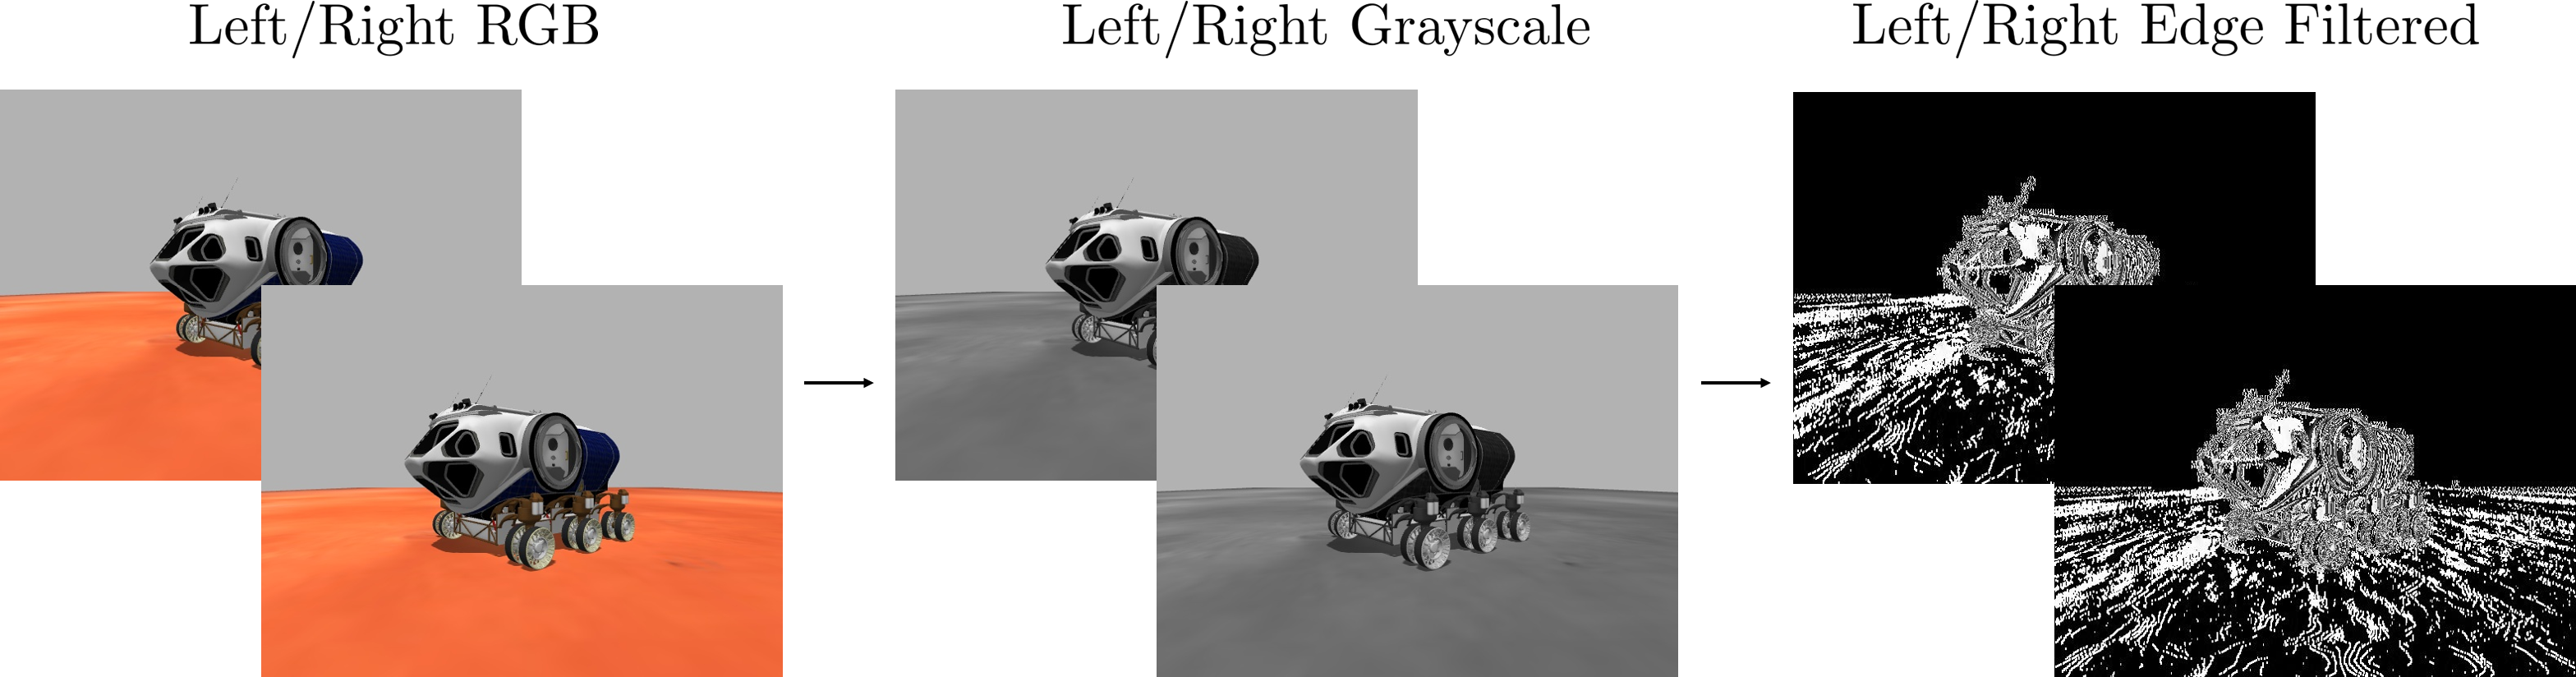
\includegraphics[scale=.28]{chapters/02_background/img/image_preprocessing.png}
	\caption{Image pre-processing to obtain edge filtered images. The images were taken within the simulation environment Gazebo (\href{http://gazebosim.org/}{\underline{link}}), and show a space exploration vehicle, for which, with the friendly support of NASA, we generated a Gazebo version (\href{https://github.com/mhubii/gazebo_models}{\underline{link}}).}
	\label{fig::224_image_preprocessing}
\end{figure}
When having a look at the Sobel kernel $\bm{S}_x$ (equation \ref{eq::224_sobel}), it immediately becomes clear that it approximates the derivative of an image along the horizontal axis. Therefore, at locations of steep change, or simply put, edges, the convolution of the grayscale images with the Sobel kernel results in high values, and thus in the typical appearance of an edge filtered image.
\begin{align}
	\bm{S}_x=
	\begin{pmatrix}
		-1 & 0 & +1 \\
		-2 & 0 & +2 \\
		-1 & 0 & +1
	\end{pmatrix}
	\label{eq::224_sobel}
\end{align}
To understand the block matching algorithm, we first need to figure out the transformation that images undergo for a change in perspective, which is caused by the two different positions of the cameras within the stereo camera pair. For an ideal setup, we have two identical cameras, and they are neither rotated relatively to each other, nor is there any other translation, but a shift along the x-axis (figure. \ref{fig::224_stereo_camera}). This may of course not always be true, and there are methods to correct for uncertainties, which we will present in the following paragraph, but omit for simplicity right now. The principle goal, for the inference of depth information from two images, is to find points in the right image that correspond to points in the left image. By triangulation, the displacement or disparity of a point in the right image, relative to its corresponding point in the left image, can then be used to extract the depth. The farther a point $\bm{X}$ lies away from the cameras, the smaller its displacement will be. In figure \ref{fig::224_stereo_camera}, we can see that a point $\bm{X}$, which is seen by the left camera, could in principle lie anywhere on the epipolar line at $\bm{x}'$, as seen from the right camera, if there is no depth information available. 
\begin{figure}[h!]
	\centering
	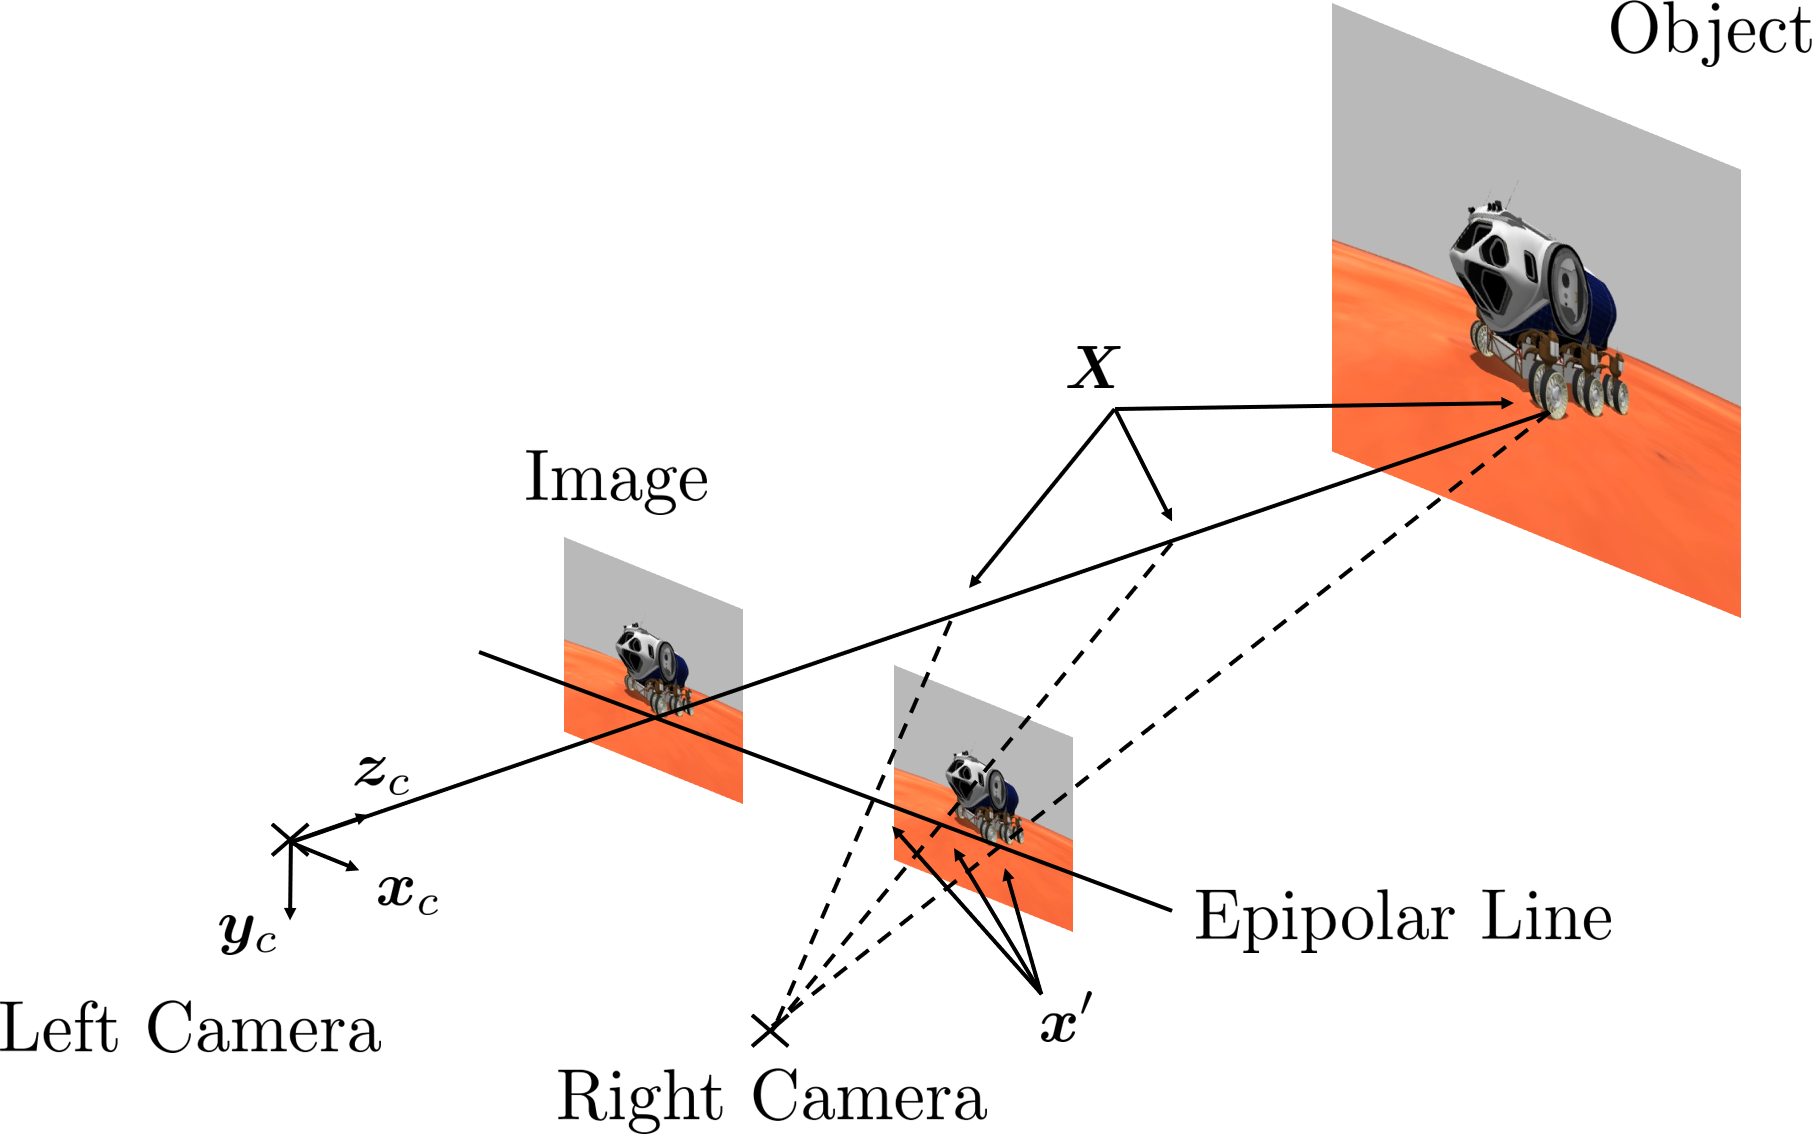
\includegraphics[scale=.28]{chapters/02_background/img/stereo_camera.png}
	\caption{The stereo setup with a left and a right camera.}
	\label{fig::224_stereo_camera}
\end{figure}
It results that, to find correspondences, one only must search along the epipolar line. Also, since points in the right image that correspond to points in the left image, will always be displaced to the left, one only must search in this direction. The procedure is shown in figure \ref{fig::224_left_disparity_map}. Instead of looking for single-pixel correspondences, it is advised to search for whole block correspondences, since it reduces the noise drastically. Blocks of a defined block size $N$ are taken from the left image, and then the sum of absolute differences SAD is computed for every displacement $d$ in the right image, ranging from zero to number of disparities $D$ (equation \ref{eq::224_sad}, figure \ref{fig::224_left_disparity_map}).
\begin{align}
	\text{SAD}(d) = \sum_{x,y=0}^N |\bm{E}_\text{left}(x,y) - \bm{E}_\text{right}(x-d,y)|
	\label{eq::224_sad}
\end{align}
The disparity $d$ that minimizes the sum of absolute differences SAD is taken to serve as the best correspondence and is therefore used in the disparity map.  Here we can already see that due to the uniqueness of the edge filtered the images $\bm{E}$, it is easier to find correspondences there, rather than in the grayscale or RGB images.
\begin{figure}[h!]
	\centering
	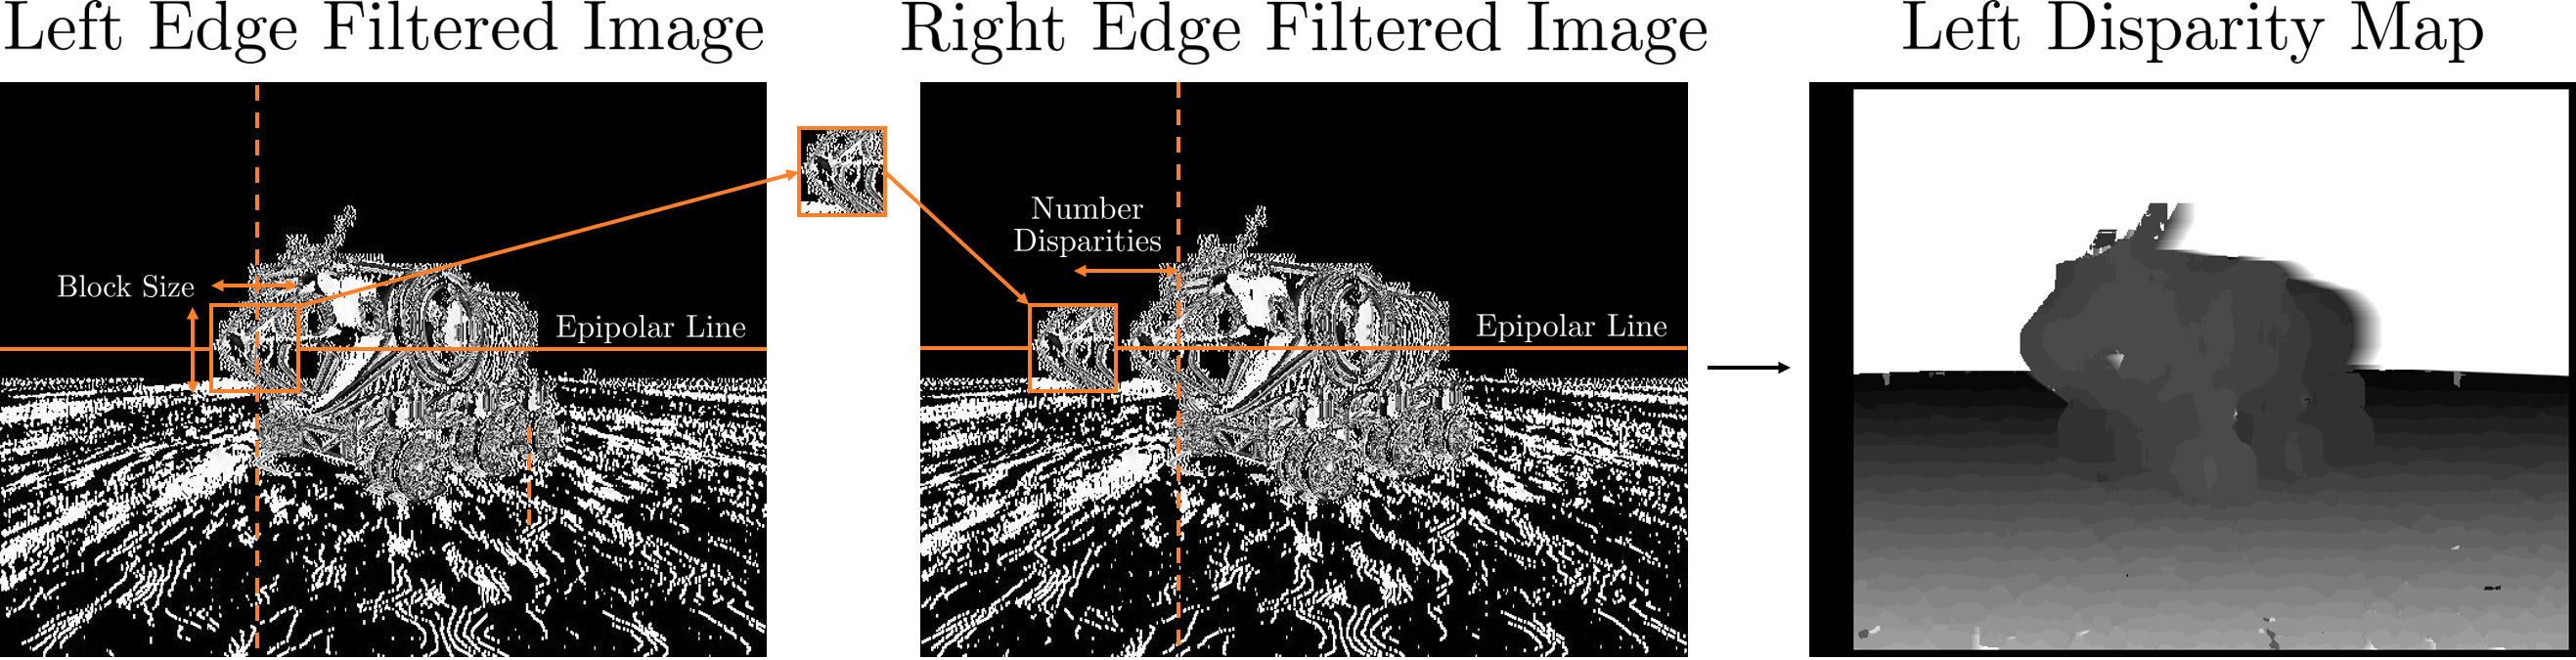
\includegraphics[scale=.28]{chapters/02_background/img/left_disparity_map.png}
	\caption{Generation of the left disparity map by the block matching algorithm.}
	\label{fig::224_left_disparity_map}
\end{figure}
To further refine the disparity map, and especially to assure good results in textureless  regions, we apply a weighted least squares filtering, which is based on the confidence of depth measures. The confidence of depth measures is obtained from the variance within the disparity map $\bm{D}$ (equation \ref{eq::224_variance}, figure \ref{fig::224_confidence_map}).
\begin{align}
	 \text{Var}(\bm{D}) = \mathbb{E}\left[\bm{D}^2\right] - \mathbb{E}\left[\bm{D}\right]^2
	\label{eq::224_variance}
\end{align} 
Therein, the expectation value for $\bm{D}$ is computed by a convolution with the kernel $\bm{K}$ from the following equation
\begin{align}
	\bm{K} &= \alpha
	\begin{pmatrix}
	1 & \dots & 1 \\
	\vdots & \ddots & \vdots \\
	1 & \dots & 1
	\end{pmatrix} \\
	\mathbb{E}\left[\bm{D}\right] &= \bm{K}*\bm{D},
	\label{eq::224_kernel}
\end{align}
where $\alpha = \frac{1}{\text{width}\cdot\text{height}}$ is the normalization factor. The expectation value of the disparity map squared $\mathbb{E}\left[\bm{D}^2\right]$ is computed in the same way, except for that all elements are squared prior to summing them up. Given the variance, we can introduce a concept which is named confidence map. The confidence map $\text{Con}(\bm{D})$ is a measure for the certainty of the computed disparity, and is defined to be linearly dependent on the variance as follows
\begin{align}
	\text{Con}(\bm{D}) = \max\left(1-r\text{Var}(\bm{D}),0\right),
\end{align}
where $r$ is a roll-off factor that defines the change of confidence with growing variance. The resulting disparity confidence is shown in figure \ref{fig::224_confidence_map} and is used to outweigh outlying disparity values from the final weighted least squares disparity map. 
\begin{figure}[h!]
	\centering
	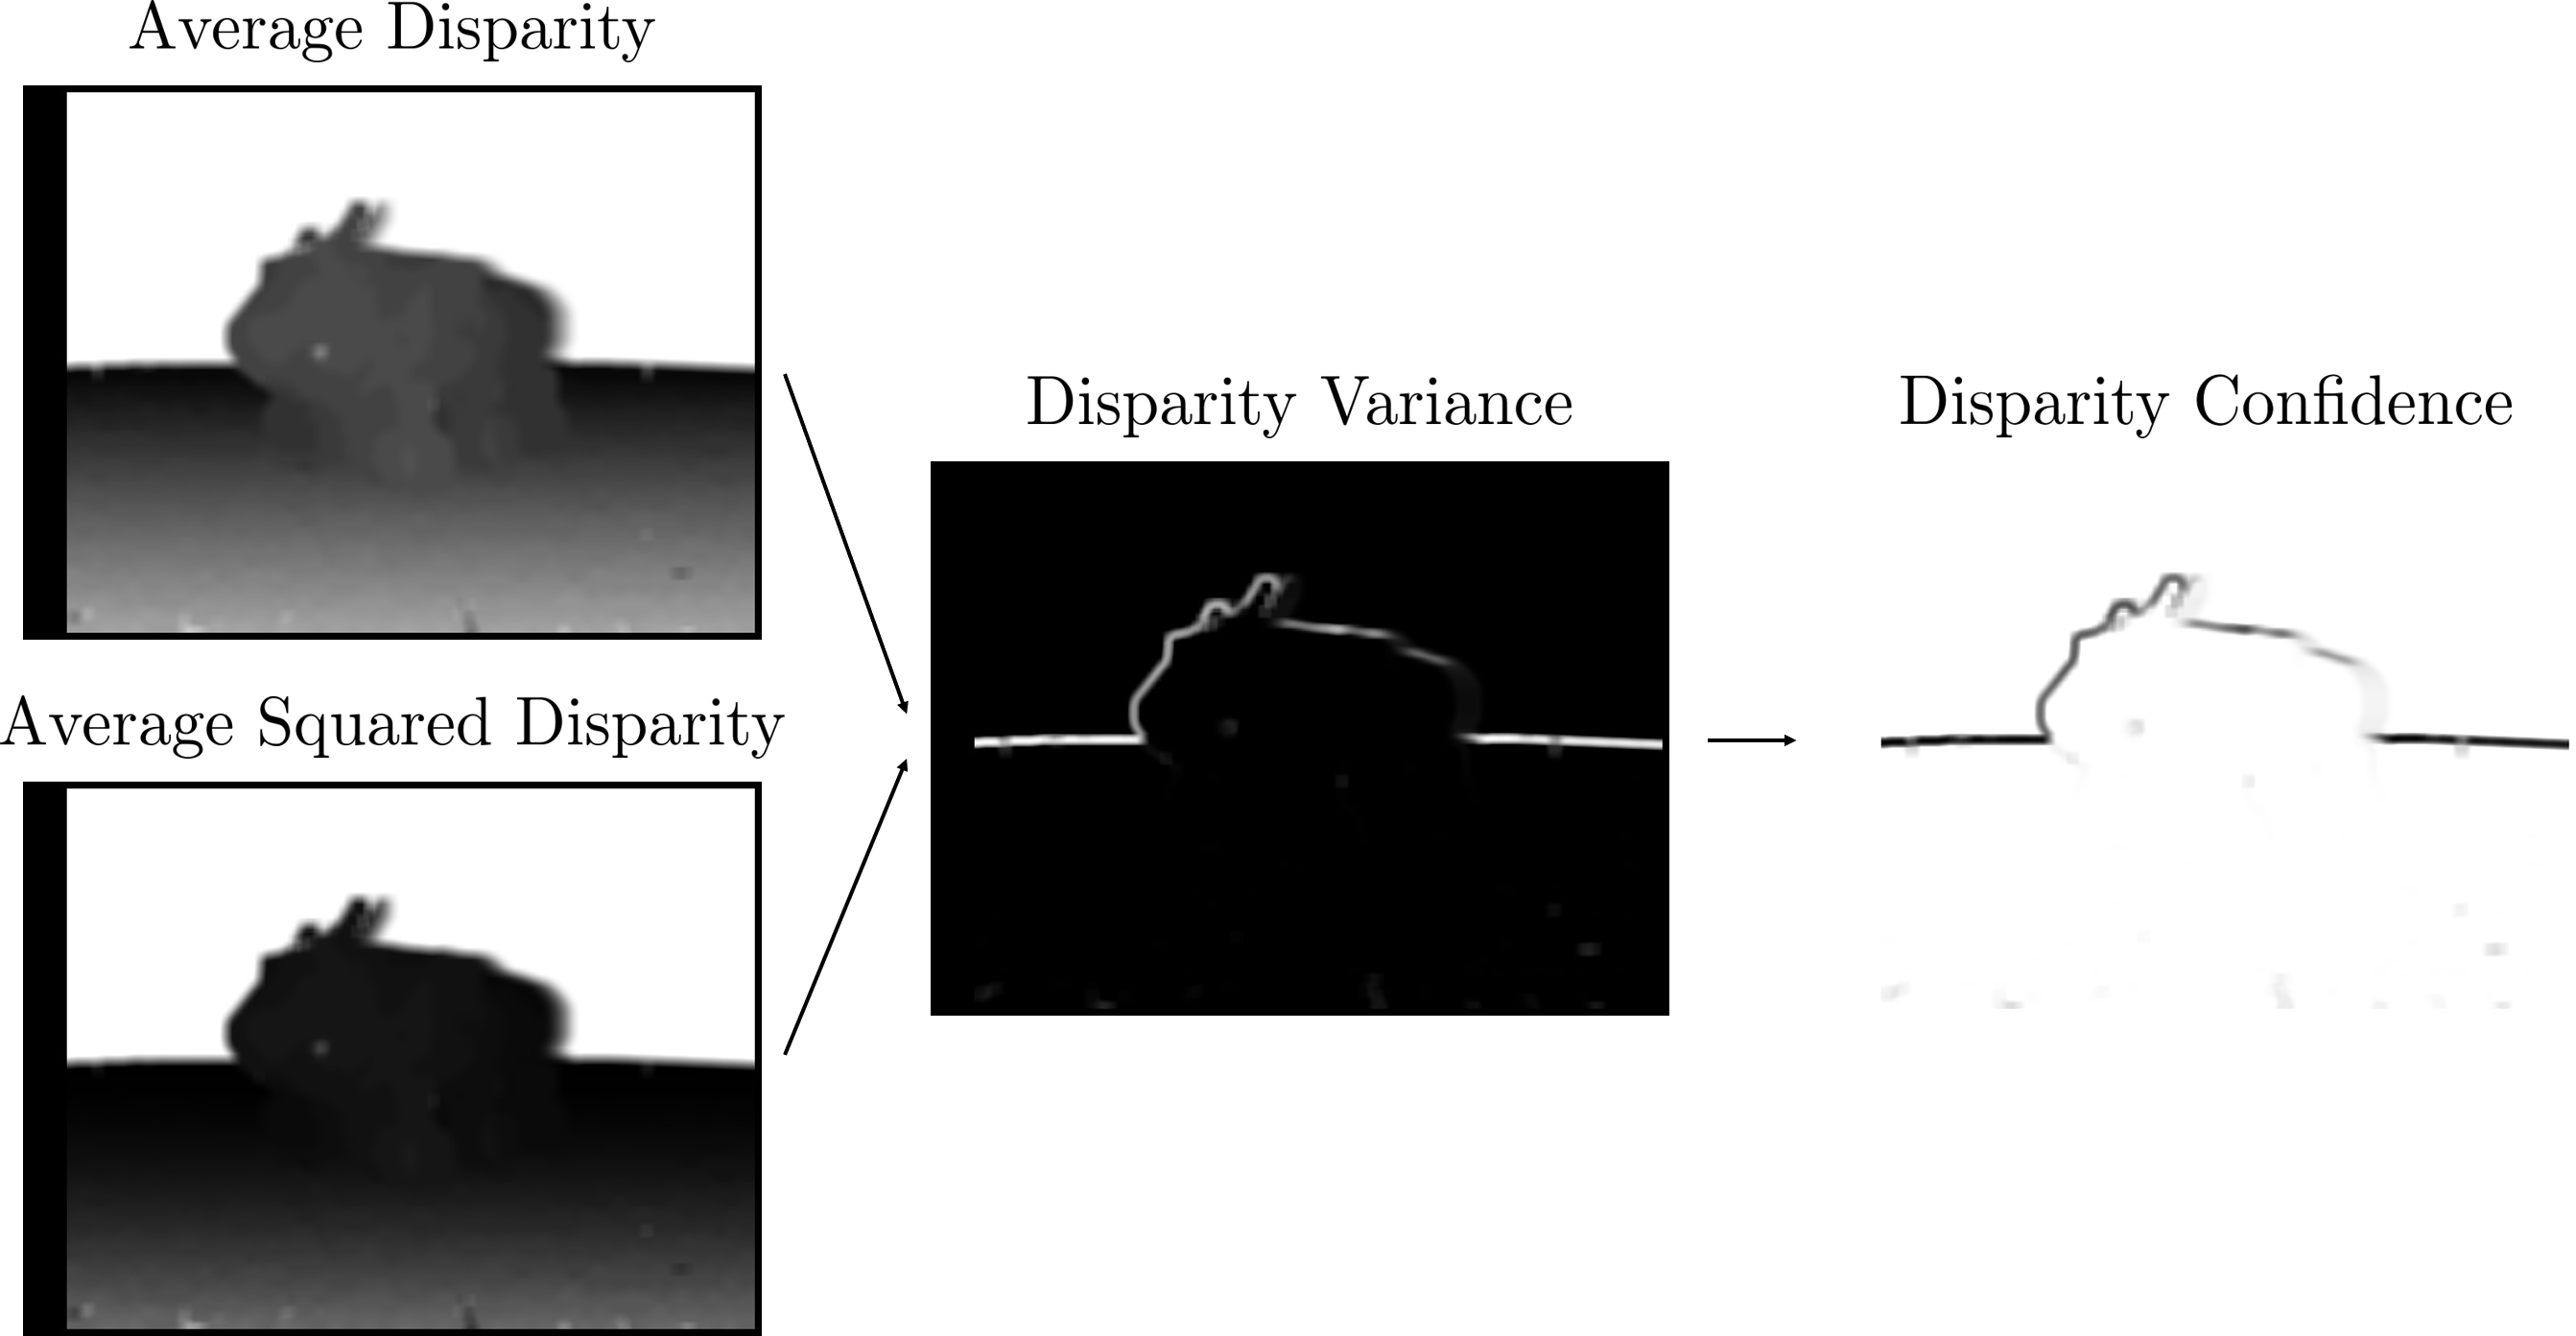
\includegraphics[scale=.28]{chapters/02_background/img/confidence_map.png}
	\caption{Generation of the confidence map from the variance within the disparity map.}
	\label{fig::224_confidence_map}
\end{figure}
Before that, we further introduce an additional measure for the prevention of accidentally assigned correspondences in the initial block matching algorithm by using a left-right consistency check \cite{egnal2004stereo}. Therefore, the block matching algorithm is used in the right image, and we search for correspondences in the left image. In contrast to the computation of the left disparity map $\bm{D}_\text{left}$, for the right disparity map $\bm{D}_\text{right}$, we only need to check for correspondences along the epipolar line in the positive displacement direction. The left-right consistency $\bm{L}$ is then obtained by 
\begin{align}
	\bm{L}(x, y) = 
	\begin{cases}
	\min \left[\text{Con}(\bm{D}_\text{left})(x, y), \text{Con}(\bm{D}_\text{right})(x + d_\text{left}, y)\right] & \text{for } \Delta d < t  \\
	0 & \text{else}
	\end{cases},
\end{align}
where $d_\text{left}$ is the disparity of $\bm{D}_\text{left}$ at position $(x,y)$, and therefore represents the index shift which results from the block matching algorithm. Furthermore, if $\Delta d = \bm{D}_\text{left}(x, y) + \bm{D}_\text{right}(x + d_\text{left}, y)$ is smaller than a threshold $t$, then the left-right consistency $\bm{L}$ is taken to be the lower bound approximation of the left and right confidences. Otherwise, the consistency is taken to be false, and hence zero (figure \ref{fig::224_weighted_least_squares_disparity}). As already pointed out, the left-right consistency, which is nothing but a confidence measure, usually reveals uncertainties in textureless regions. The weighted least squares filtering that we are about to present uses this fact to its advantage. In a first step, a consistency weighted disparity map $\bm{C}$ is computed via equation \ref{eq::224_cwd} (figure \ref{fig::224_weighted_least_squares_disparity}).
\begin{align}
	\bm{C}=\bm{L}\cdot\bm{D}_\text{left},
	\label{eq::224_cwd}
\end{align}
where $\cdot$ is an element-wise multiplication. Further, the weighted least squares filter is based on the idea of a bilateral filter \cite{tomasi1998bilateral}, and it will try to minimize an energy function $J(\bm{U})$, which takes the original grayscale image as guidance to compute a weight $w_{p,q}$ for neighboring pixels $p$, and $q$ as follows
\begin{align}
	w_{x,y,i,j}(g) = exp(-|g_{x,y}-g_{i,j}|/\sigma).
	\label{eq::224_weight}
\end{align}
Depending on the range parameter $\sigma$, this weight will be high for similar neighboring pixels of the grayscale image $g$, and therefore lead to huge costs in the following energy function $J(\bm{U})$ that we try to minimize
\begin{align}
	J(\bm{U}) = \sum_{x,y}\left[(u_{x,y}-c_{x,y})^2+\lambda\sum_{(i,j)\in\mathcal{N}(x,y)}w_{x,y,i,j}(g)(u_{x,y}-u_{i,j})^2\right],
	\label{eq::224_energy_function}
\end{align}
where $c_{x,y}$ are single pixels of the consistency weighted disparity map. The formulation of this energy function results in a solution $\bm{U}$ that encourages the propagation of disparity values from high- to low-confidence regions (figure \ref{fig::224_weighted_least_squares_disparity}). Additionally, the weight $w$, together with the smoothing parameter $\lambda$, ensure to have similar disparity values in regions with similar texture. The final disparity map $\bm{D}_\text{final}$ is then obtained by normalizing the resulting image $\bm{U}$ with
\begin{align}
	\bm{D}_\text{final} = \frac{\bm{U}}{\text{WLS}(\bm{L})},
	\label{eq::224_wls_final}
\end{align}
where $\text{WLS}(\bm{U})$ is the weighted least squares filtered version of the left-right consistency $\bm{L}$.
\begin{figure}[h!]
	\centering
	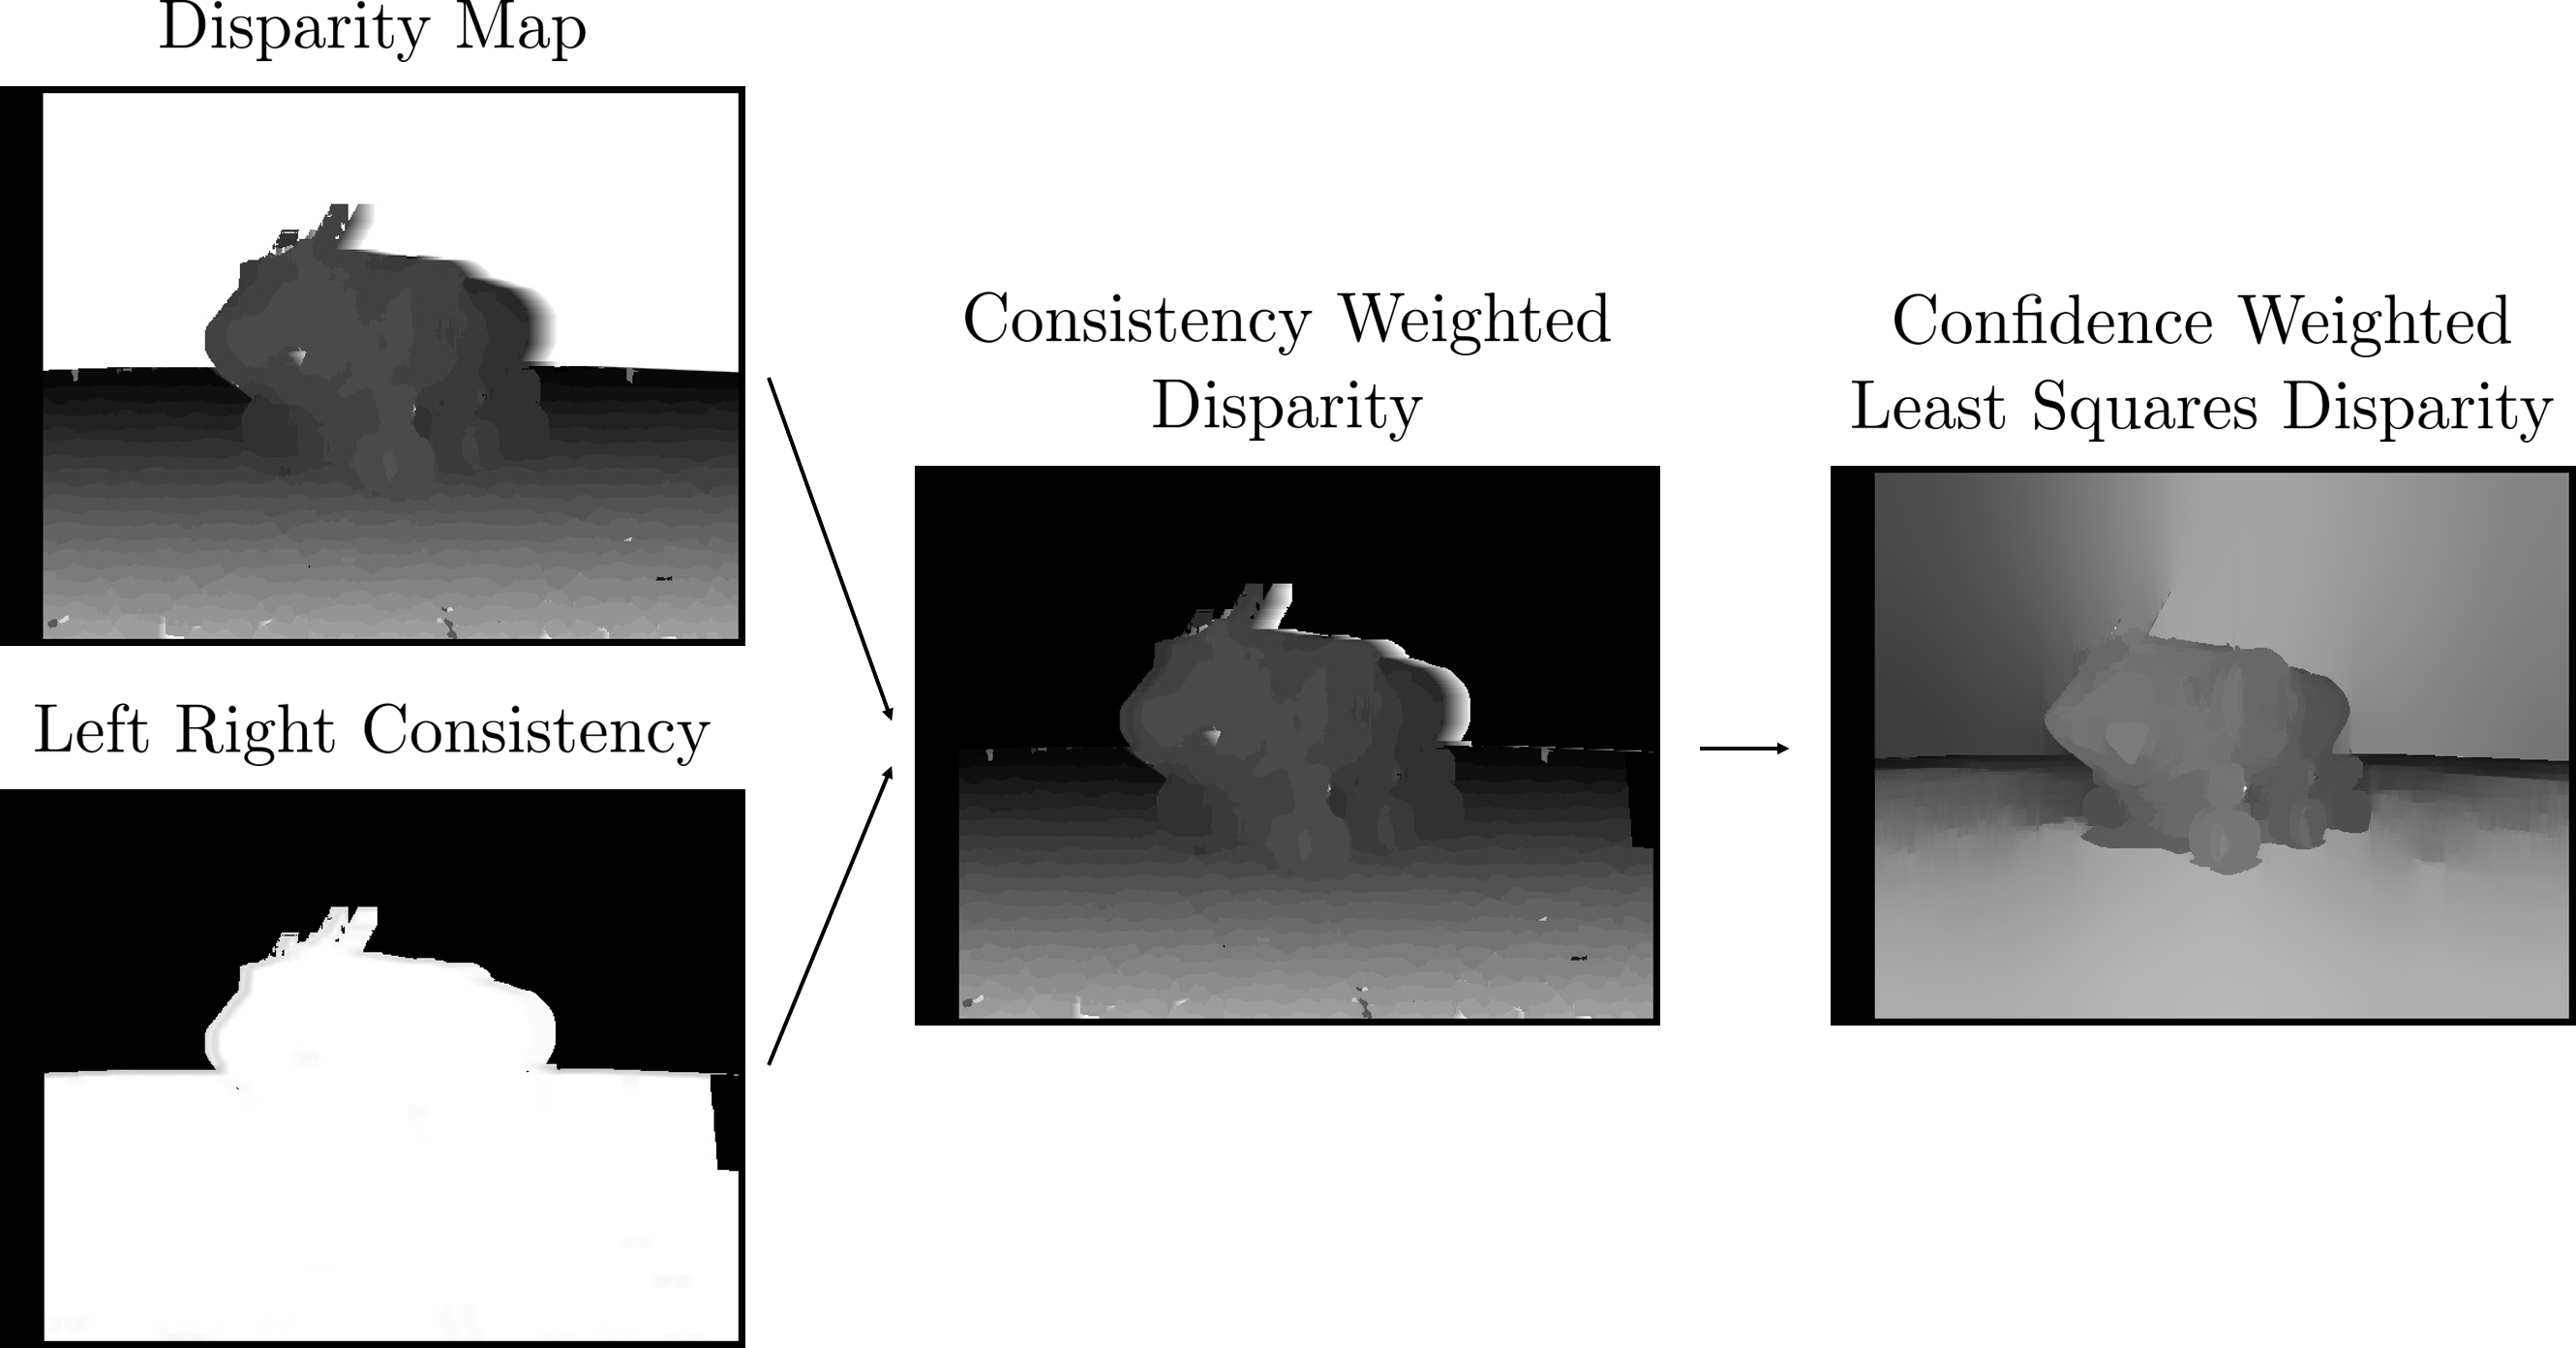
\includegraphics[scale=.28]{chapters/02_background/img/weighted_least_squares_disparity.png}
	\caption{Generation of the confidence weighted least squares disparity from the disparity map, and the left-right consistency.}
	\label{fig::224_weighted_least_squares_disparity}
\end{figure}
\\\\
As already mentioned in figure \ref{fig::224_stereo_camera}, the assumption of an only translated stereo camera pair is rarely correct. Besides, there exist camera intrinsics that deform the observed image, and so the epipolar lines. Therefore, as a requirement for the algorithm to work properly, it is important to calibrate the robot's cameras. The next chapter - Mono and Stereo Camera Calibration, will explain in detail how this is done.
\FloatBarrier
\subsubsection{Mono and Stereo Camera Calibration}
To correct images, as we observe them with a camera, it is required to have a mathematical description of it. A simple one for a camera is the pinhole model, which is shown in figure \ref{fig::224_pin_hole_camera}. For a pinhole camera model, the image plane lies behind the coordinate frame of the camera, and is turned the other way around, but it is easier to describe the image in a virtual plane, which is located at a distance $f$ along the $z_c$-axis, where $f$ is the focal length.
\begin{figure}[h!]
	\centering
	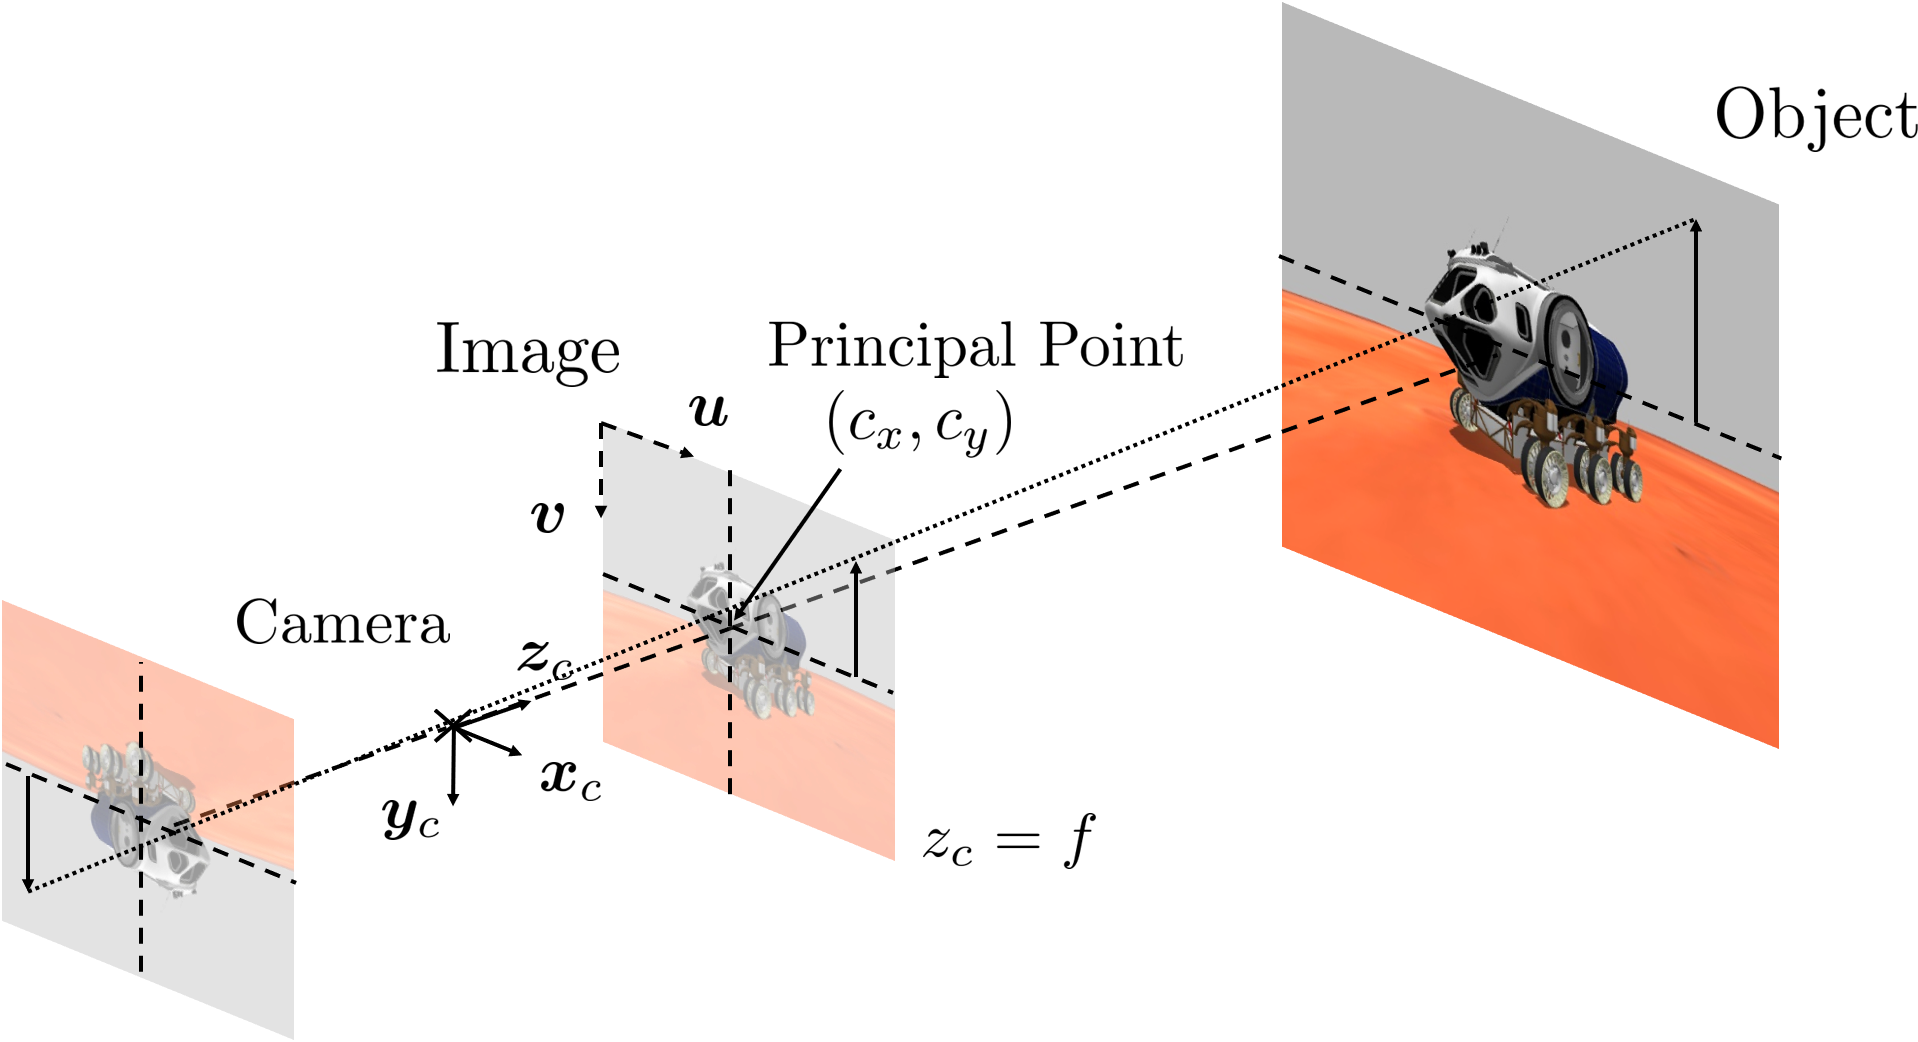
\includegraphics[scale=.28]{chapters/02_background/img/pin_hole_camera.png}
	\caption{Pinhole camera model.}
	\label{fig::224_pin_hole_camera}
\end{figure}
According to the intercept theorem, a point $\bm{X}_c = (X,Y,Z)^T$ is then simply projected to the image plane by the camera matrix $\bm{K}$ with
\begin{align}
	\bm{x}_c = \bm{K}\bm{X}_c = \begin{pmatrix}
	f_x & 0   & c_x \\
	0   & f_y & c_y \\
	0   & 0   & 1
	\end{pmatrix}\bm{X}_c.
	\label{eq::224_focal_intrinsics}
\end{align}
Therein, $\bm{K}$ contains the intrinsic camera parameters, such as the focal lengths and the principal point. For a true pinhole camera $f_x = f_y =f$, but due to errors, usually two different values are chosen. The principal point lies at the position where a light ray connects perpendicularly to the image plane after passing the pinhole, and therefore just defines an offset. For a real setup, it is also required to put a lens at the pinhole's position, which adds some distortion to the image. According to \cite{duane1971close}, we model radial and tangential distortion by
\begin{align}
	x_{c,u} &= x_{c,d}(1+k_1r^2+k_2r^4+k_3r^6) + p_1(r^2+2x_{c,d}^2) + 2p_2x_{c,d}y_{c,d} 
	\label{eq::224_x_dist}\\
	y_{c,u} &= x_{c,d}(1+k_1r^2+k_2r^4+k_3r^6) + 2p_1x_{c,d}y_{c,d} + p_2(r^2+2y_{c,d}^2),
	\label{eq::224_y_dist}
\end{align}
where
\begin{align}
	(x_{c,d}, y_{c,d}) = &\,\,\text{distorted image points within the camera frame $c$,} 
	\nonumber\\
		                 &\,\,\text{as projected onto the image plane}
	\nonumber\\ 
	(x_{c,u}, y_{c,u}) = &\,\,\text{undistorted image points within the camera frame $c$,}
	\nonumber\\
	                     &\,\,\text{as projected by an ideal pinhole camera}
	\nonumber\\
	k_n = &\,\,\text{n$^\text{th}$ radial distortion coefficient}
	\nonumber\\
	p_n = &\,\,\text{n$^\text{th}$ tangential distortion coefficient}
	\nonumber\\
	r = &\,\,\sqrt{x_{c,d}^2+y_{c,d}^2}.
	\nonumber
\end{align}
Together, the focal lengths, the principal point, and the distortion coefficients make up the unknowns within our camera model. Goal of the mono camera calibration is now to find these coefficients from images of a well-known calibration pattern. Therefore, images of the calibration pattern are taken from different perspectives (figure \ref{fig::224_calibration_process}). 
\begin{figure}[h!]
	\centering
	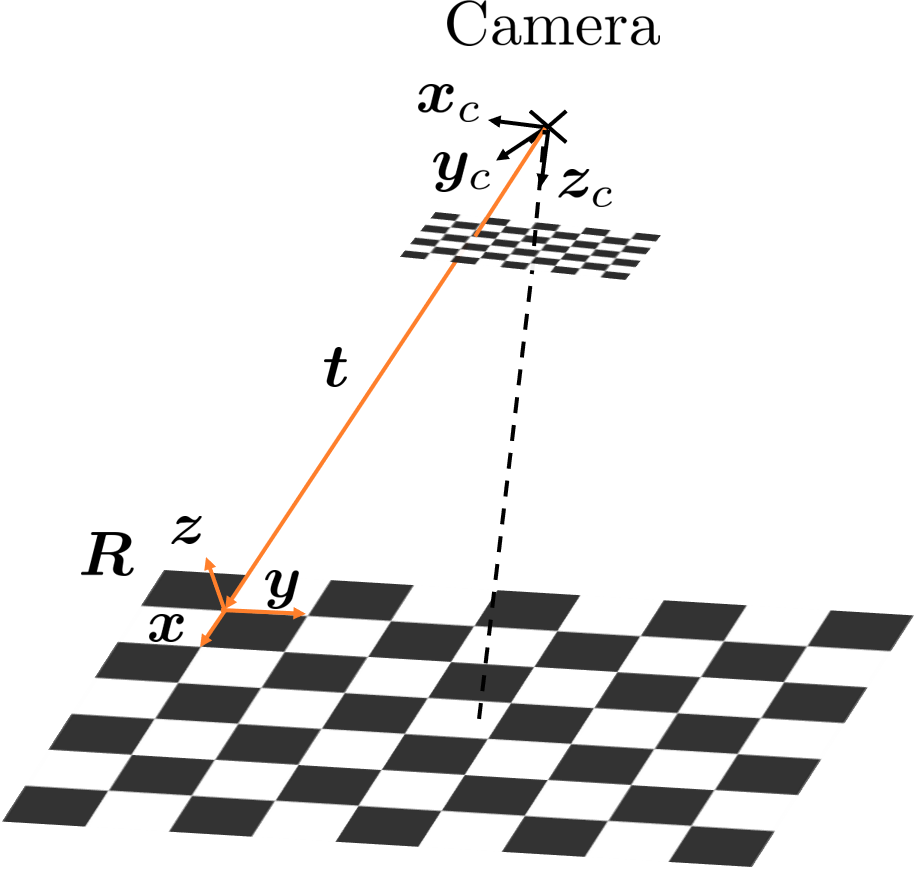
\includegraphics[scale=.28]{chapters/02_background/img/calibration_process.png}
	\caption{Calibration pattern, as observed from the camera's coordinate system $C$. Within the object's coordinate system, all chessboard corners lie at a zero $z$-position.}
	\label{fig::224_calibration_process}
\end{figure}
For the mathematical description, the calibration pattern is taken to be at a fixed position and orientation, while it is assumed that the camera was moved. The position of each corner can then be described by the square's size $a$ as follows
\begin{align}
	\bm{x}_{nm} = \begin{pmatrix}
	wa & ha & 0 & 1
	\end{pmatrix}^T,
	\label{eq::224_square_size}
\end{align}
where we now switched to homogeneous coordinates, and $w\in[0,W],h\in[0,H]$ are whole numbers, corresponding to the width and the height of the pattern. It is then required to find the rotation $\bm{R}$ and translation $\bm{t}$, which transforms the object points to the image plane. They are estimated by solving a perspective-n-point problem \cite{fischler1981random}. Therefore, as shown in figure \ref{fig::224_distortion} (b), a corner detecting algorithm finds the corners $\bm{x}_{c,wh}$ within the image plane. Under the assumption of known intrinsic camera parameters, $\bm{x}_{c,wh}$ are then being undistorted according to equations \ref{eq::224_x_dist} and \ref{eq::224_y_dist}. 
\begin{figure}[h!]
	\centering
	\subcaptionbox{}%
	[.4\linewidth]{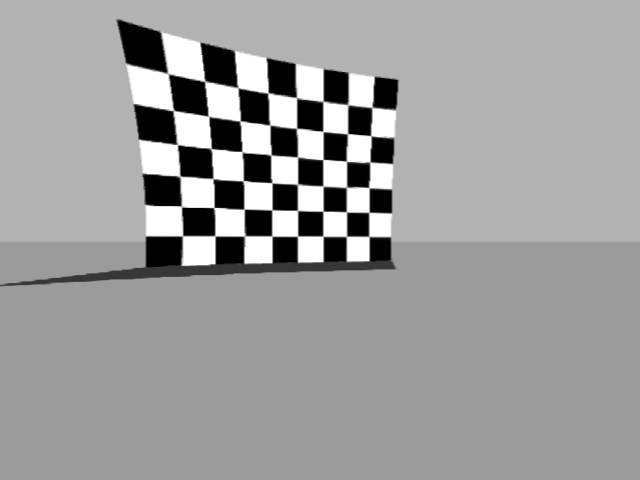
\includegraphics[scale=.2]{chapters/02_background/img/gazebo_calib_left.jpg}}
	\subcaptionbox{}%
	[.4\linewidth]{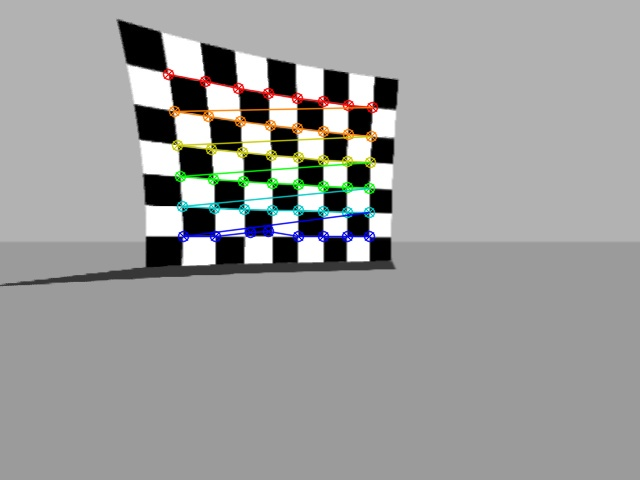
\includegraphics[scale=.2]{chapters/02_background/img/gazebo_corners.jpg}}
	\caption{Distorted calibration pattern (a), and the image points as found by the algorithm (b).}
	\label{fig::224_distortion}
\end{figure} 
Each $\bm{x}_{nm}$ can then be transformed to the camera's frame, and further be projected onto the image plane via
\begin{align}
	\bm{x}_{c,wh} = \bm{K}\begin{pmatrix}
	\bm{R} & \bm{t}
	\end{pmatrix}\bm{x}_{wh},
\end{align}
where $\bm{R}$ describes the rotation, and $\bm{t}$ the translation of the camera frame to the object frame. Then, equations \ref{eq::224_x_dist} and \ref{eq::224_y_dist} are applied to obtain the undistorted image points from $\bm{x}_{c,wh}$. The undistorted image points $\bm{x}_{c,wh,u}$ are then being reprojected by inverting the rotation and translation via
\begin{align}
	\bm{x}_{wh,u} = \begin{pmatrix}
	\bm{R} & \bm{t}
	\end{pmatrix}^{-1}\bm{x}_{c,wh,u},
	\label{eq::224_reprojection}
\end{align}
from which we compute the re-projection error $\Delta x = ||\bm{x}_{wh,u} - \bm{x}_{wh}||_2$. To find the intrinsic parameters, a Levenberg-Marquardt algorithm then optimizes them in an iterative scheme to minimize the re-projection error until convergence \cite{zhang2000flexible}. The stereo camera calibration can then be performed by applying the mono camera calibration to each camera separately, from which the camera intrinsics are obtained. Given the camera intrinsics of both cameras, it is again possible to solve a perspective-n-point problem, which yields the positions and orientations of both cameras with respect to the observed object. This enables us to compute the fundamental matrix $\bm{F}$, which transforms points from the left camera's view $\bm{x}_{c_\text{left}}$, to points $\bm{x}_{c_\text{right}}$, as seen by the right camera via
\begin{align}
	\bm{x}_{c_\text{right}}^T\bm{F}\bm{x}_{c_\text{left}} = \bm{0}
\end{align}
The mapping enables us to rectify the left and the right image \cite{loop1999computing}, using the rectification transforms $\bm{R}_i$, which means that we can compute homography transforms that align epipolar lines within the images (figure \ref{fig::224_rectified}), which were previously defined by the fundamental matrix. 
\begin{figure}[h!]
	\centering
	\subcaptionbox{}%
	[.4\linewidth]{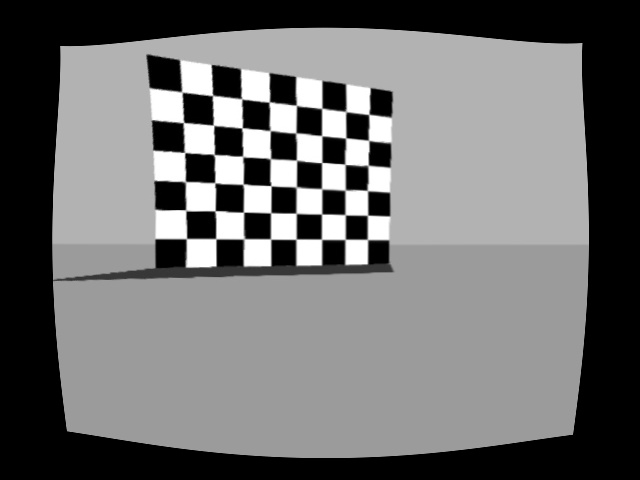
\includegraphics[scale=.2]{chapters/02_background/img/gazebo_rectified_left.jpg}}
	\subcaptionbox{}%
	[.4\linewidth]{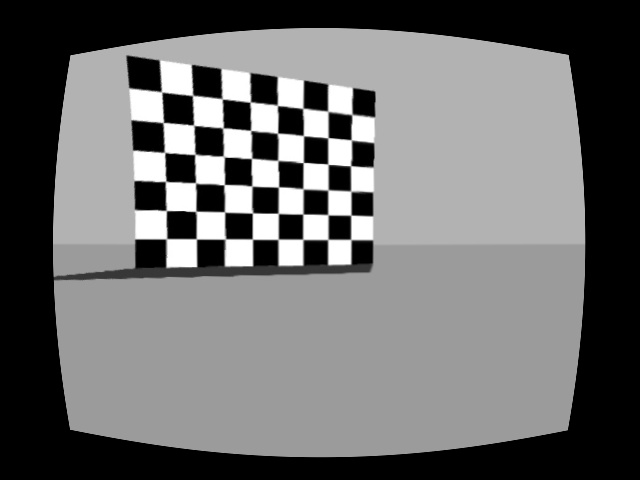
\includegraphics[scale=.2]{chapters/02_background/img/gazebo_rectified_right.jpg}}
	\caption{Undistorted calibration pattern, as observed by the left camera (a), and by the right camera (b). For comparison, see the distorted calibration pattern in figure \ref{fig::224_distortion}, and note how the horizons within the images align.}
	\label{fig::224_rectified}
\end{figure}
These homography transforms map the images, as we observe them with the cameras, to a shared virtual plane, which is defined by the newly obtained projection matrices $\bm{P}_i$. Therefore, we reached our initial goal, since it enables us to apply the stereo block matching algorithm, which got introduced earlier, to the transformed images.   % image processing
	
	\chapter{Methods}
	While there is an extensive guide on the installation of the implemented software within the appendix \ref{sec::A_si}, the purpose of this chapter is to give the future reader a good understanding of it. The code itself was written generically, such that it is not dependent on the used robot at all, for why it is very well suited to perform future research on arbitrary humanoid robots with. Therefore, the reader will be given a broad overview of the overall code's structure in section \ref{sec::31_cs}, in order to allow for a fast assessment of possibly reusable implementations. The completely decoupled pattern generation and deep learning parts of the software are hence explained first in section \ref{sec::32_pg}, and section \ref{sec::33_dl}, respectively. Following that, the particular communication with our humanoid robot will be explained in section \ref{sec::34_co}.








	\FloatBarrier
\section{Code Structure}
\label{sec::31_cs}
As shown in figure \ref{fig::31_folder}, there are four main folders within the implemented code. Those include the libraries inside the libs folder, the models, among them Heicub's URDF model for computing kinematics, and another one for pure visualization with MeshUp \cite{meshup}, the sh folder, which contains shell scripts for easy execution, and furthermore the source folder, which relies on the libraries to build executables from. And while these executables are very much dependent on the robot at hand, as they are coupled to the robot's communication system, they pose some nice examples on how the pattern generator can be embedded into a robot's operating system. Now in order to reuse the code for a different robot, one could either install the libraries and include the headers, as explained in section \ref{sec::A1_pg}, or replace the input-output module (io\_module) by a new one and keep the folder's structure. Nonetheless, we will only focus on the libraries' usage by introducing simple examples in the following sections and keep the details of implementation on a different operating system up to the future reader. We will further bridge the gap between the background of section \ref{sec::2_bg} by explaining the different methods, which we implemented, and we will further highlight its correlation with the YAML \cite{ben2005yaml} configuration files that can be found as building block of each library. 
\begin{figure}[h!]
\begin{forest}
	for tree={
		font=\ttfamily,
		grow'=0,
		child anchor=west,
		parent anchor=south,
		anchor=west,
		calign=first,
		edge path={
			\noexpand\path [draw, \forestoption{edge}]
			(!u.south west) +(7.5pt,0) |- node[fill,inner sep=1.25pt] {} (.child anchor)\forestoption{edge label};
		},
		before typesetting nodes={
			if n=1
			{insert before={[,phantom]}}
			{}
		},
		fit=band,
		before computing xy={l=15pt},
	}
	[\href{https://github.com/mhubii/nmpc_pattern_generator}{\underline{nmpc\_pattern\_generator}}
	[\href{https://github.com/mhubii/nmpc_pattern_generator/tree/master/libs}{\underline{libs}}
	[\href{https://github.com/mhubii/nmpc_pattern_generator/tree/master/libs/io_module}{\underline{io\_module}}
	[\href{https://github.com/mhubii/nmpc_pattern_generator/tree/master/libs/io_module/include/io_module}{\underline{include/io\_module}}[reader.h][writer.h]]
	[configs.yaml][cam\_stereo.yaml]]
	[\href{https://github.com/mhubii/nmpc_pattern_generator/tree/master/libs/kinematics}{\underline{kinematics}}[\href{https://github.com/mhubii/nmpc_pattern_generator/tree/master/libs/kinematics/include/kinematics}{\underline{include/kinematics}}[kinematics.h]][configs.yaml]
	]
	[
	\href{https://github.com/mhubii/nmpc_pattern_generator/tree/master/libs/learning}{\underline{learning}}[\href{https://github.com/mhubii/nmpc_pattern_generator/tree/master/libs/learning/include/learning}{\underline{include/learning}}[models.h][proximal\_policy\_optimization.h]][\href{https://github.com/mhubii/nmpc_pattern_generator/tree/master/libs/learning/python}{\underline{python}}]
	]
	[\href{https://github.com/mhubii/nmpc_pattern_generator/tree/master/libs/pattern_generator}{\underline{pattern\_generator}}[\href{https://github.com/mhubii/nmpc_pattern_generator/tree/master/libs/pattern_generator/include/pattern_generator}{\underline{include/pattern\_generator}}[base\_generator.h][interpolation.h][nmpc\_generator.h]]
	[configs.yaml]]
	]
	[\href{https://github.com/mhubii/nmpc_pattern_generator/tree/master/models}{\underline{models}}]
	[\href{https://github.com/mhubii/nmpc_pattern_generator/tree/master/sh}{\underline{sh}}]
	[\href{https://github.com/mhubii/nmpc_pattern_generator/tree/master/src}{\underline{src}}]
	]
\end{forest}
\caption{Folder structure of the code, which got implemented for this thesis. The code is freely available on GitHub at the provided \href{https://github.com/mhubii/nmpc_pattern_generator}{\underline{link}}. Install instruction can be found in the appendix \ref{sec::A_si}.}
\label{fig::31_folder}
\end{figure}

	\section{Pattern Generation}
\label{sec::32_pg}
lalal
\begin{minipage}{1.\textwidth}
	\begin{minipage}{0.3\textwidth}
		\scriptsize{
			\hfill Specifications\\
			\mbox{}~\hfill 1\\
			\mbox{}~\hfill 1\\
			\mbox{}~\hfill 1\\
			\mbox{}~\hfill 1\\
			\mbox{}~\hfill 1\\
			\mbox{}~\hfill 1\\
			\mbox{}~\hfill 1\\
			
			\hfill Interpolation\\
			\mbox{}~\hfill 1\\
			\mbox{}~\hfill 1\\
			\mbox{}~\hfill 1\\
			\mbox{}~\hfill 1\\
			
			\hfill Initial Values\\
			\mbox{}~\hfill 1\\
			\mbox{}~\hfill 1\\
			\mbox{}~\hfill 1\\
			\mbox{}~\hfill 1\\
			\mbox{}~\hfill 1\\
			\mbox{}~\hfill 1\\
			\mbox{}~\hfill 1\\
			\mbox{}~\hfill 1\\
			
			\hfill Environment\\
			\mbox{}~\hfill 1\\
			
			\hfill Obstacle\\
			\mbox{}~\hfill 1\\
			\mbox{}~\hfill 1\\
			\mbox{}~\hfill 1\\
			\mbox{}~\hfill 1\\
			
			\hfill Optimization\\
			\mbox{}~\hfill 1\\
			\mbox{}~\hfill 1\\
			\mbox{}~\hfill 1\\
			\mbox{}~\hfill 1\\
			\mbox{}~\hfill 1\\
			\mbox{}~\hfill 1\\
			\mbox{}~\hfill 1\\
			\mbox{}~\hfill 1}
	\end{minipage}
	\begin{minipage}{0.7\textwidth}
		\begin{lstlisting}[language=yaml]
# Specifications.
t_step: 3.2
security_margin: [0.02, 0.02]
left_foot_convex_hull: [-0.11, 0.14, ...]
right_foot_convex_hull: [-0.11, -0.14, ...]
foot_width: 0.1
foot_length: 0.2
foot_distance: 0.14

# Interpolation.
command_period: 0.01
n_still: 0
t_ds: 1.6
step_height: 0.03

# Initial values.
com_x: [0.0 , 0.0, 0.0]
com_y: [0.05, 0.0, 0.0]
com_z: 0.45
com_q: [0.0 , 0.0, 0.0]
support_foot: left
foot_x: 0.0
foot_y: 0.07
foot_q: 0.0

# Environment.
gravity: 9.81

# Obstacle.
obstacle: false
x_pos:  10
y_pos:  10
radius: 0.5

# Optimization.
n: 16
t: 0.4
t_feedback: 0.4
alpha: 1
beta: 1e2
gamma: 1e-2
cpu_time: 0.1
nwsr: 1000
		\end{lstlisting}
	\end{minipage}
	\captionof{table}{The configurations YAML file for the pattern generator. It can be found at the provided \href{https://github.com/mhubii/nmpc_pattern_generator/blob/master/libs/pattern_generator/configs.yaml}{\underline{link}}.}
\end{minipage}
\cite{eigenweb} % eigen
\cite{ferreau2014qpoases} % qpOASES
\cite{felis2017rbdl} %rbdl
\cite{googletest} % gtest
\cite{opencv_library}
\cite{paszke2017automatic} % pytorch
\begin{minipage}{1.\textwidth}
	\begin{minipage}{0.3\textwidth}
		\scriptsize{
			\hfill URDF Model\\
			\mbox{}~\hfill 1\\
			
			\hfill Initial Inverse Kinematic Runs\\
			\mbox{}~\hfill 1\\
			
			\hfill Inverse Kinematic Parameters\\
			\mbox{}~\hfill 1\\
			\mbox{}~\hfill 1\\
			\mbox{}~\hfill 1\\
			
			\hfill Body Points\\
			\mbox{}~\hfill 1\\
			\mbox{}~\hfill 1\\
			\mbox{}~\hfill 1}
	\end{minipage}
	\begin{minipage}{0.7\textwidth}
		\begin{lstlisting}[language=yaml]
# Location of the urdf model.
urdf_loc: ../../models/icub_heidelberg01_no_weights.urdf

# Number of pre-initializations for inverse kinematics.
n_init: 10

# Parameters for the inverse kinematics.
step_tol: 1e-12
lambda: 1e-2
num_steps: 1000

# Body points.
com_body_point: [0.0, 0.0, 0.0]
lf_body_point: [0.0, 0.0, 0.0]
rf_body_point: [0.0, 0.0, 0.0]
		\end{lstlisting}
	\end{minipage}
	\captionof{table}{The configurations YAML file for the kinematics. It can be found at the provided \href{https://github.com/mhubii/nmpc_pattern_generator/blob/master/libs/kinematics/configs.yaml}{\underline{link}}.}
\end{minipage}

	\FloatBarrier
\section{Deep Learning Integration}
\label{sec::33_dl}
Yet again, the first step within the deep learning pipeline is the image processing, as already introduced in section  \ref{sec::224_ip}. The camera calibration within this work was done using OpenCV \cite{opencv_library}. Exemplary code with which we did the depth map parameter tuning in section \ref{sec::422_dp}, can be found at the provided \href{https://github.com/mhubii/nmpc_pattern_generator/blob/master/src/tune_disp_map.cpp}{\underline{link}}. It relies on the rectification matrices $\bm{R}_i$, and the projection matrices $\bm{P}_i$ that got explained in section \ref{sec::224_ip}. These are stored as YAML files inside of the io\_module folder of figure \ref{fig::31_folder}. They are highly dependent on the robot but will not change for Heicub over time, for why the future reader will be able to reuse them. As already explained in section \ref{sec::222_bc}, Heicub's recorded images and the corresponding velocities got stored inside of a folder. A text file was created in the cause of this process, which stored the locations to the image files, as well as the velocities. For a faster prototyping, we then decided to implement the deep learning training pipeline within Python with PyTorch \cite{paszke2017automatic}, for which the routine can be found at the provided \href{https://github.com/mhubii/nmpc_pattern_generator/blob/master/libs/learning/python/train_rgbd.py}{\underline{link}}. The trained model got then converted to a just in time (JIT) script that was loaded into the executables in the src folder of figure \ref{fig::31_folder} via
\begin{minted}{cpp}
  auto module = torch::jit::load(net_location);
\end{minted}
The code to convert a model, which got trained in Python, to C++, is part of the python folder and can be found at the following \href{https://github.com/mhubii/nmpc_pattern_generator/blob/master/libs/learning/python/python_to_cpp.py}{\underline{link}}. For Heicub, there was an additional step to be done, which is explained in section \ref{sec::34_co}, but given the camera images and depth maps are provided as \inlinecode{C++}{cv::Mat}, it is possible to convert them to a \inlinecode{C++}{torch::Tensor}, which can then be concatenated into a single RGBD tensor. We temporarily saved a sequence of these tensors, which enabled us to forward them through our long short term memory based neural network, for which the architecture is given in figure \ref{fig::423_unet}. For the behavioral augmentation, this can for example be seen at the provided \href{https://github.com/mhubii/nmpc_pattern_generator/blob/719fde0bb73925923de85cbf379c5523e075dfeb/src/behavioural_augmentation_real_robot_external_data.cpp#L625}{\underline{link}}. Once the neural network predicts a desired velocity for the pattern generation, one only has to convert the desired velocity back to an \inlinecode{C++}{Eigen::Vector3d}, which is the datatype that the pattern generation library works with. This velocity is then forwarded, just as described in section \ref{sec::32_pg}, via the \inlinecode{}{NMPCPatternGenerator::SetVelocityReference} method, and a new iteration is executed. In the following section we will explain how the developed pipelines can be used together with Heicub. It is therefore mainly required to implement the control loop of figure \ref{fig::2_cl}. 
	\section{Heicub}
\label{sec::34_he}
Heicub is a descendant of the iCub, which was especially designed for optimal control in locomotion at the Istituto Italiano di Tecnologia in Genova. It is used within this thesis to test the implemented algorithms, for which it provides all the required actuators and sensors. As shown in figure \ref{fig::34_hei} (c), Heicub has a total of 21 degrees of freedom, of which 6 correspond to the floating base, and 15 to the rotational joints. Its two RGB cameras have a resolution of $240\times320$ pixels at a framerate of $60\,\text{fps}$, and are located within the chest, as shown in figure \ref{fig::34_hei} (a). The force torque sensors, with which we compute the zero moment point, are located within the ankles and the hip. According to equations \ref{eq::211_x_pos_zmp_simp} and \ref{eq::211_y_pos_zmp_simp}, we only require the force torque sensors from the ankles, where $d=0.03\,\text{m}$. Heicub also supports skin sensors, and an inertial measurement unit, but both are not used within this thesis. The use of the robot, and all its sensors, is well described within the appendix, starting from section \ref{sec::B_su}. Furthermore, Heicub has a Gazebo simulation model, which is shown in figure \ref{fig::34_hei}, and for which the installation instruction can be found in section \ref{sec::A4_sm}. It provides the exact same functionality as its real equivalent does. This is achieved via Gazebo plugins, which communicate to the YARP network, just as Heicub does. The plugins can be installed by following the instructions in section \ref{sec::a52_plugins}. The Gazebo model offers a perfect environment for software development, as we can make sure that implemented algorithms work properly, prior to their usage on the real robot, which could take harm from wrongly designed software. YARP stands short for Yet Another Robot Platform, and its installation is explained in section \ref{sec::a52_yarp}. Most important for us is to understand the YARP network in more detail, as it allows us to communicate to the robot. It is therefore explained within the next section - Communication with Heicub.
\begin{figure}[h!]
	\centering
	\subcaptionbox{Heicub.}%
	[.3\linewidth]{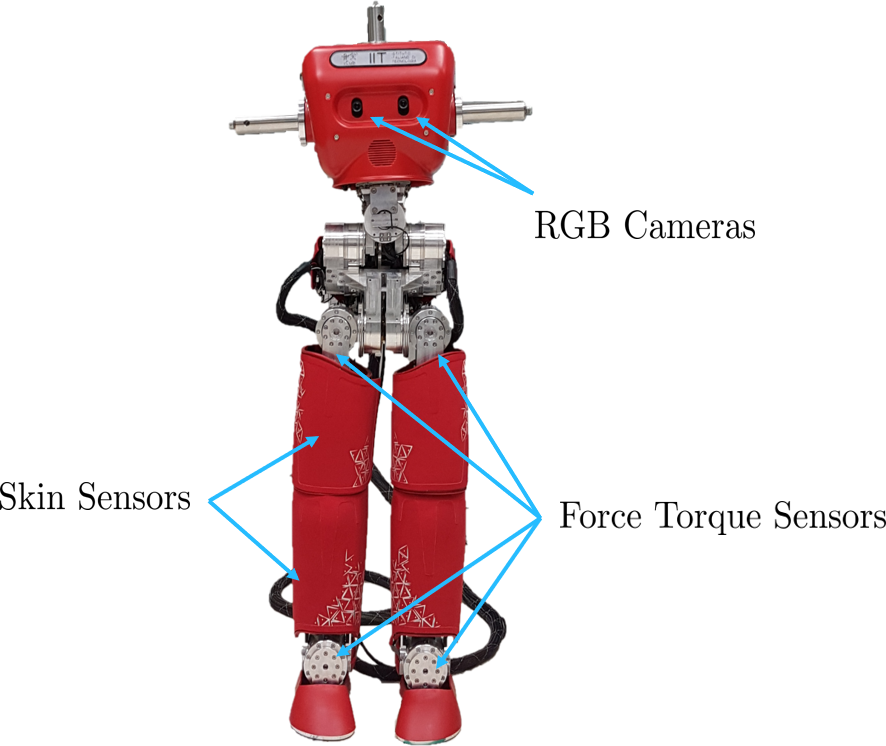
\includegraphics[scale=.35]{chapters/03_methods/img/heicub.png}}
	\subcaptionbox{Gazebo model.}%
	[.3\linewidth]{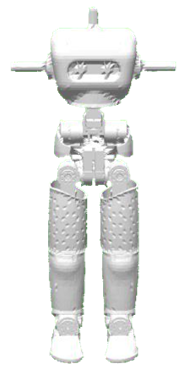
\includegraphics[scale=.35]{chapters/03_methods/img/gazebo_heicub.png}}
	\subcaptionbox{Kinematic chain.}%
	[.3\linewidth]{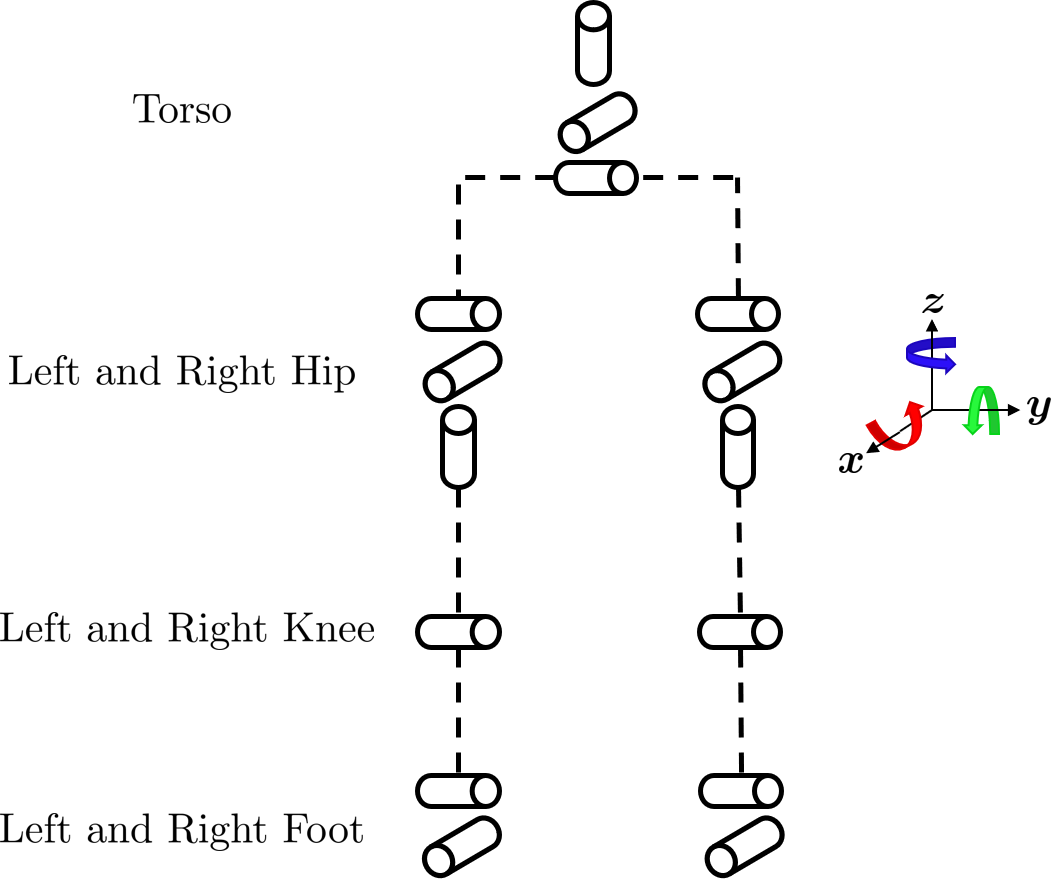
\includegraphics[scale=.35]{chapters/03_methods/img/kinematic_tree.png}}
	\caption{Heicub, the robot, which we used for the evaluation of the implemented software. There exists the real robot (a), as well as a simulated version of it, which offer equivalent functionality (b). Heicub's degrees of freedom, which can be actuated, are shown in (c). All the joints are rotational joints.}
	\label{fig::34_hei}
\end{figure}
\FloatBarrier
\subsection{Communication with Heicub}
\label{sec::341_co}
With YARP \cite{metta2006yarp}, it is possible to directly interface the robot's motors, the cameras, and the force torque sensors. Moreover, it enables the user to run multiple programs in parallel, which can then communicate with each other, which is of special importance for the control loop that was implemented within the scope of this thesis (see figure \ref{fig::341_yarp}).
\begin{figure}[h!]
	\hspace*{-1cm}
	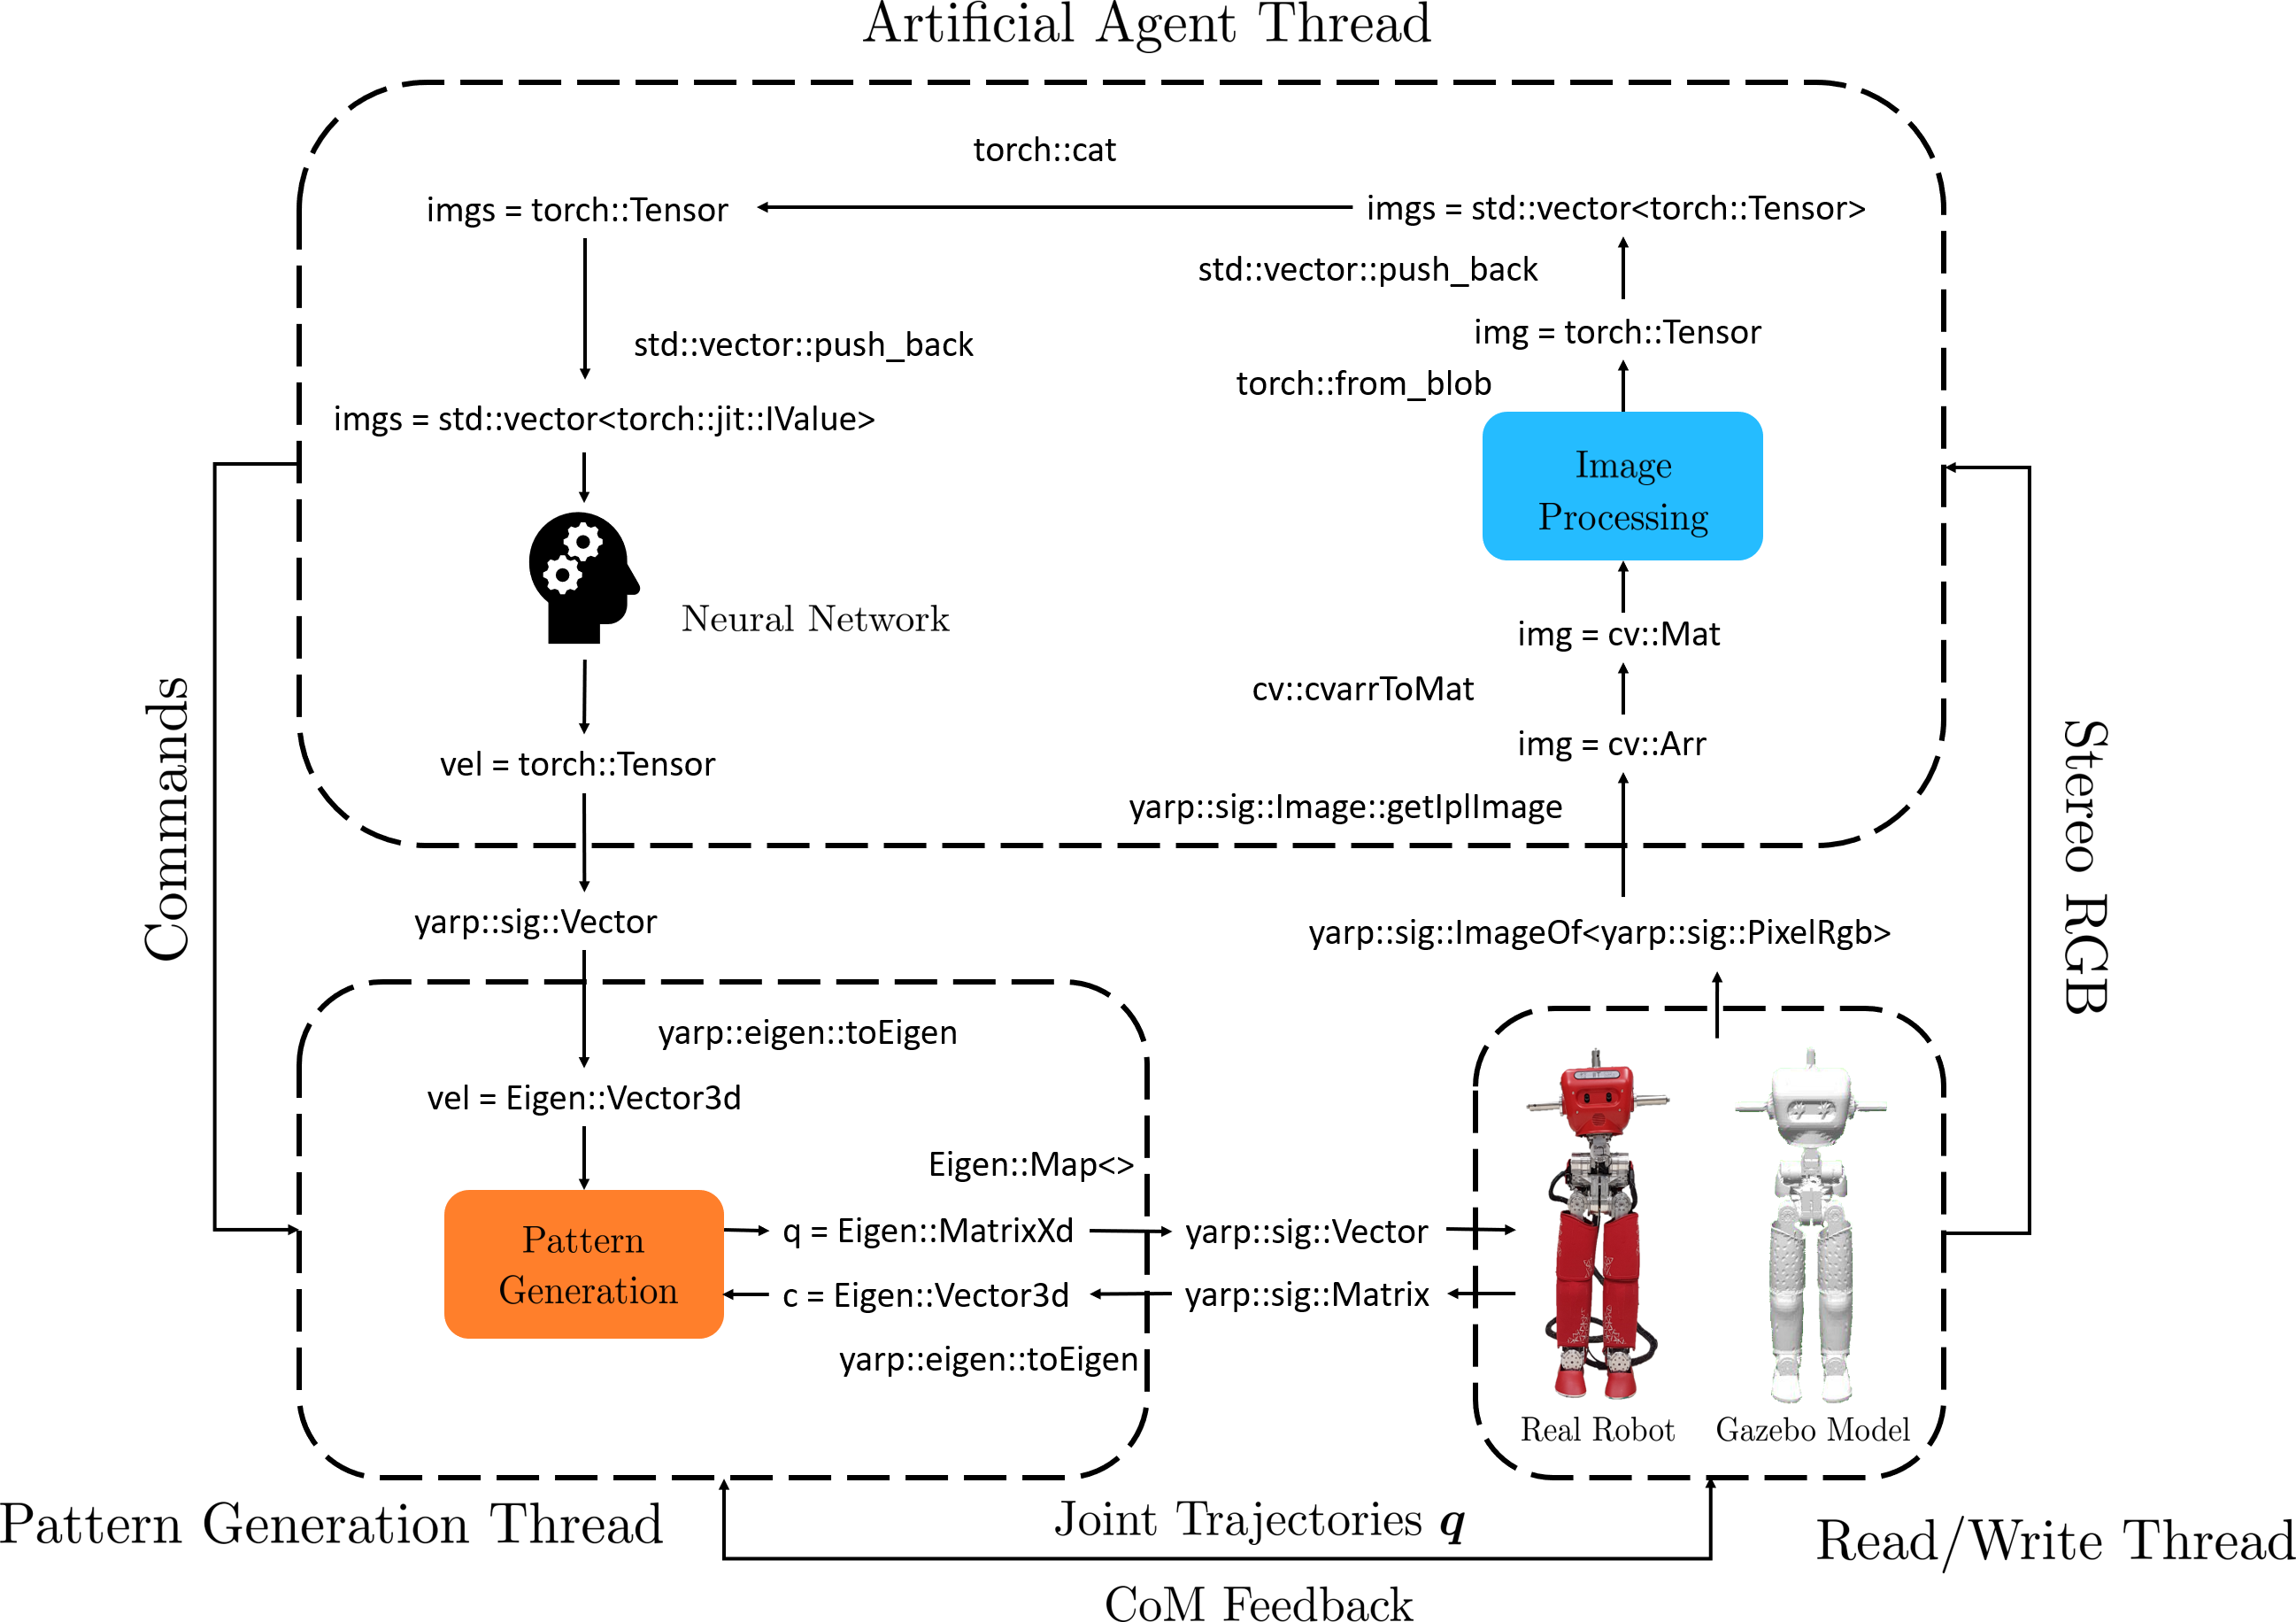
\includegraphics[scale=.4]{chapters/03_methods/img/yarp_diag.png}
	\caption{YARP is used to run multiple threads in parallel, each of which is indicated by the dashed boxes. It further enables the individual threads to communicate with each other via ports, which exchange YARP objects. It enables communication to the real robot as well as to a simulated version of it. The diagram demonstrates the types of data, which are being used, and the functions that convert them. Notice that this is an extended version of figure \ref{fig::2_cl}.}
	\label{fig::341_yarp}
\end{figure}
As we know from the previous section, one of these threads is committed to take decisions with a neural network, given RGBD images. This thread is depicted as the artificial agent thread in figure \ref{fig::341_yarp}. The pattern generation thread performs the nonlinear model predictive control, given the velocity command of the artificial agent thread. Furthermore, there are two additional running threads that communicate with Heicub's motors. These threads are the read, and the write thread in figure \ref{fig::341_yarp}. The classes, which implement the communication to the robot, are located within the io\_module folder of figure \ref{fig::31_folder}. The \inlinecode{C++}{WriteJoints} class implements a \inlinecode{C++}{yarp::os::RateThread}, which is periodically being called, to accesses the motors, which are defined within the YAML configuration file, and changes the motors' settings to position direct mode. Therefore, whatever is being written to the port that \inlinecode{C++}{WriteJoints} uses to communicate with the YARP network, and which is defined in the YAML configuration file, directly gets executed on the robot's motors. This communication to Heicub's motors corresponds to the very lowest part of figure \ref{fig::341_yarp}, where, as extensively explain in section \ref{sec::32_pg}, the pattern generation uses the forward kinematics to generate joint angles $\bm{q}$, which are being written as \inlinecode{C++}{yarp::sig::Vector} to the \inlinecode{C++}{WriteJoints} rate thread. The reading of the robot's sensors is also implemented as part of the io\_module folder in figure \ref{fig::31_folder}. There are several classes, which implement \inlinecode{C++}{yarp::os::RateThread}s for different reading tasks. Among them are the \inlinecode{C++}{ReadJoints} class, which reads out the motor encoders to obtain the joint angles, the \inlinecode{C++}{ReadCameras} class, which reads out the cameras and pushes them as \inlinecode{C++}{yarp::sig::ImageOf<yarp::sig::PixelRgb>} onto the network (see figure \ref{fig::341_yarp}), as well as the \inlinecode{C++}{AppReader} class, and the \inlinecode{C++}{KeyReader} class, which handle the communication to the joystick app, and the terminal, respectively. Both, the \inlinecode{C++}{AppReader} class, and the \inlinecode{C++}{KeyReader} class, utilize NCurses to generate a user interface on the terminal, which is internally being trapped in a while loop until exit. They readout the input, which may originate from the joystick app, or the keyboard, and push them as the velocity commands onto the YARP network (see figure \ref{fig::341_yarp} left). The velocity commands, which are converted into an \inlinecode{C++}{Eigen::Vector3d} for the \inlinecode{C++}{NMPCGenerator::SetVelocityReference} method from section \ref{sec::32_pg}, may alternatively also originate from a neural network, which is being presented in figure \ref{fig::341_yarp}. The \inlinecode{C++}{GenerateVelocityCommands} rate thread, which enables this feature, is implemented as part of the src folder in \ref{fig::31_folder}, as it only utilizes the provided libraries. It can be found at the provided \href{https://github.com/mhubii/nmpc_pattern_generator/blob/719fde0bb73925923de85cbf379c5523e075dfeb/src/behavioural_augmentation_real_robot_external_data.cpp#L108}{\underline{link}}. Its main task is to read in the images, which are constantly being pushed to the YARP network by \inlinecode{C++}{ReadCameras}, and to convert them into \inlinecode{C++}{cv::Mat} matrices, for us to perform the image processing on them, which includes the rectification, and the depth map extraction that are explained in section \ref{sec::224_ip}. The \inlinecode{C++}{GenerateVelocityCommands} class additionally stores a sequence of the processed images in the form of a \inlinecode{C++}{std::vector<torch::Tensor>}. Whenever a new image is read from the YARP network, the oldest image within the \inlinecode{C++}{std::vector<torch::Tensor>} is being deleted, and all other images are shifted up by one index, such that the newest image is available as the first entry. This vector of tensors is then being converted into a single tensor, by concatenating the individual tensors along the first dimension, which is, by definition of the long short-term memory units, required in PyTorch. The concatenated tensor is further being converted into a \inlinecode{C++}{std::vector<torch::jit::IValue>}, such that the JIT script, which defines the neural network that got trained in Python (see \ref{sec::33_dl}), can forward it. The output is then obtained as a \inlinecode{C++}{torch::Tensor} yet again, which is being written in the form of a \inlinecode{C++}{yarp::sig::Vector} to the YARP network, such that,  as explained above, the pattern generation can use it as input. This pipeline works equivalently on the real robot, as well as on a simulated version of it in Gazebo \cite{koenig2004design}, for which install instructions are provided in the appendix \ref{sec::A4_sm}. Although it allowed us to prototype within the simulation, we will use the pipeline to train the real robot Heicub, as an example for our method, on finding a fire extinguisher within the next section - Experiments.
	\FloatBarrier
\section{Communication with Heicub}
\label{sec::35_co}
With YARP \cite{metta2006yarp}, it is possible to directly interface the robot's motors, the cameras, and the force torque sensors. Moreover, it enables the user to run multiple programs in parallel, which can then communicate with each other, which is of special importance for the control loop that was implemented within the scope of this thesis (see figure \ref{fig::35_yarp}).
\begin{figure}[h!]
	\hspace*{-1cm}
	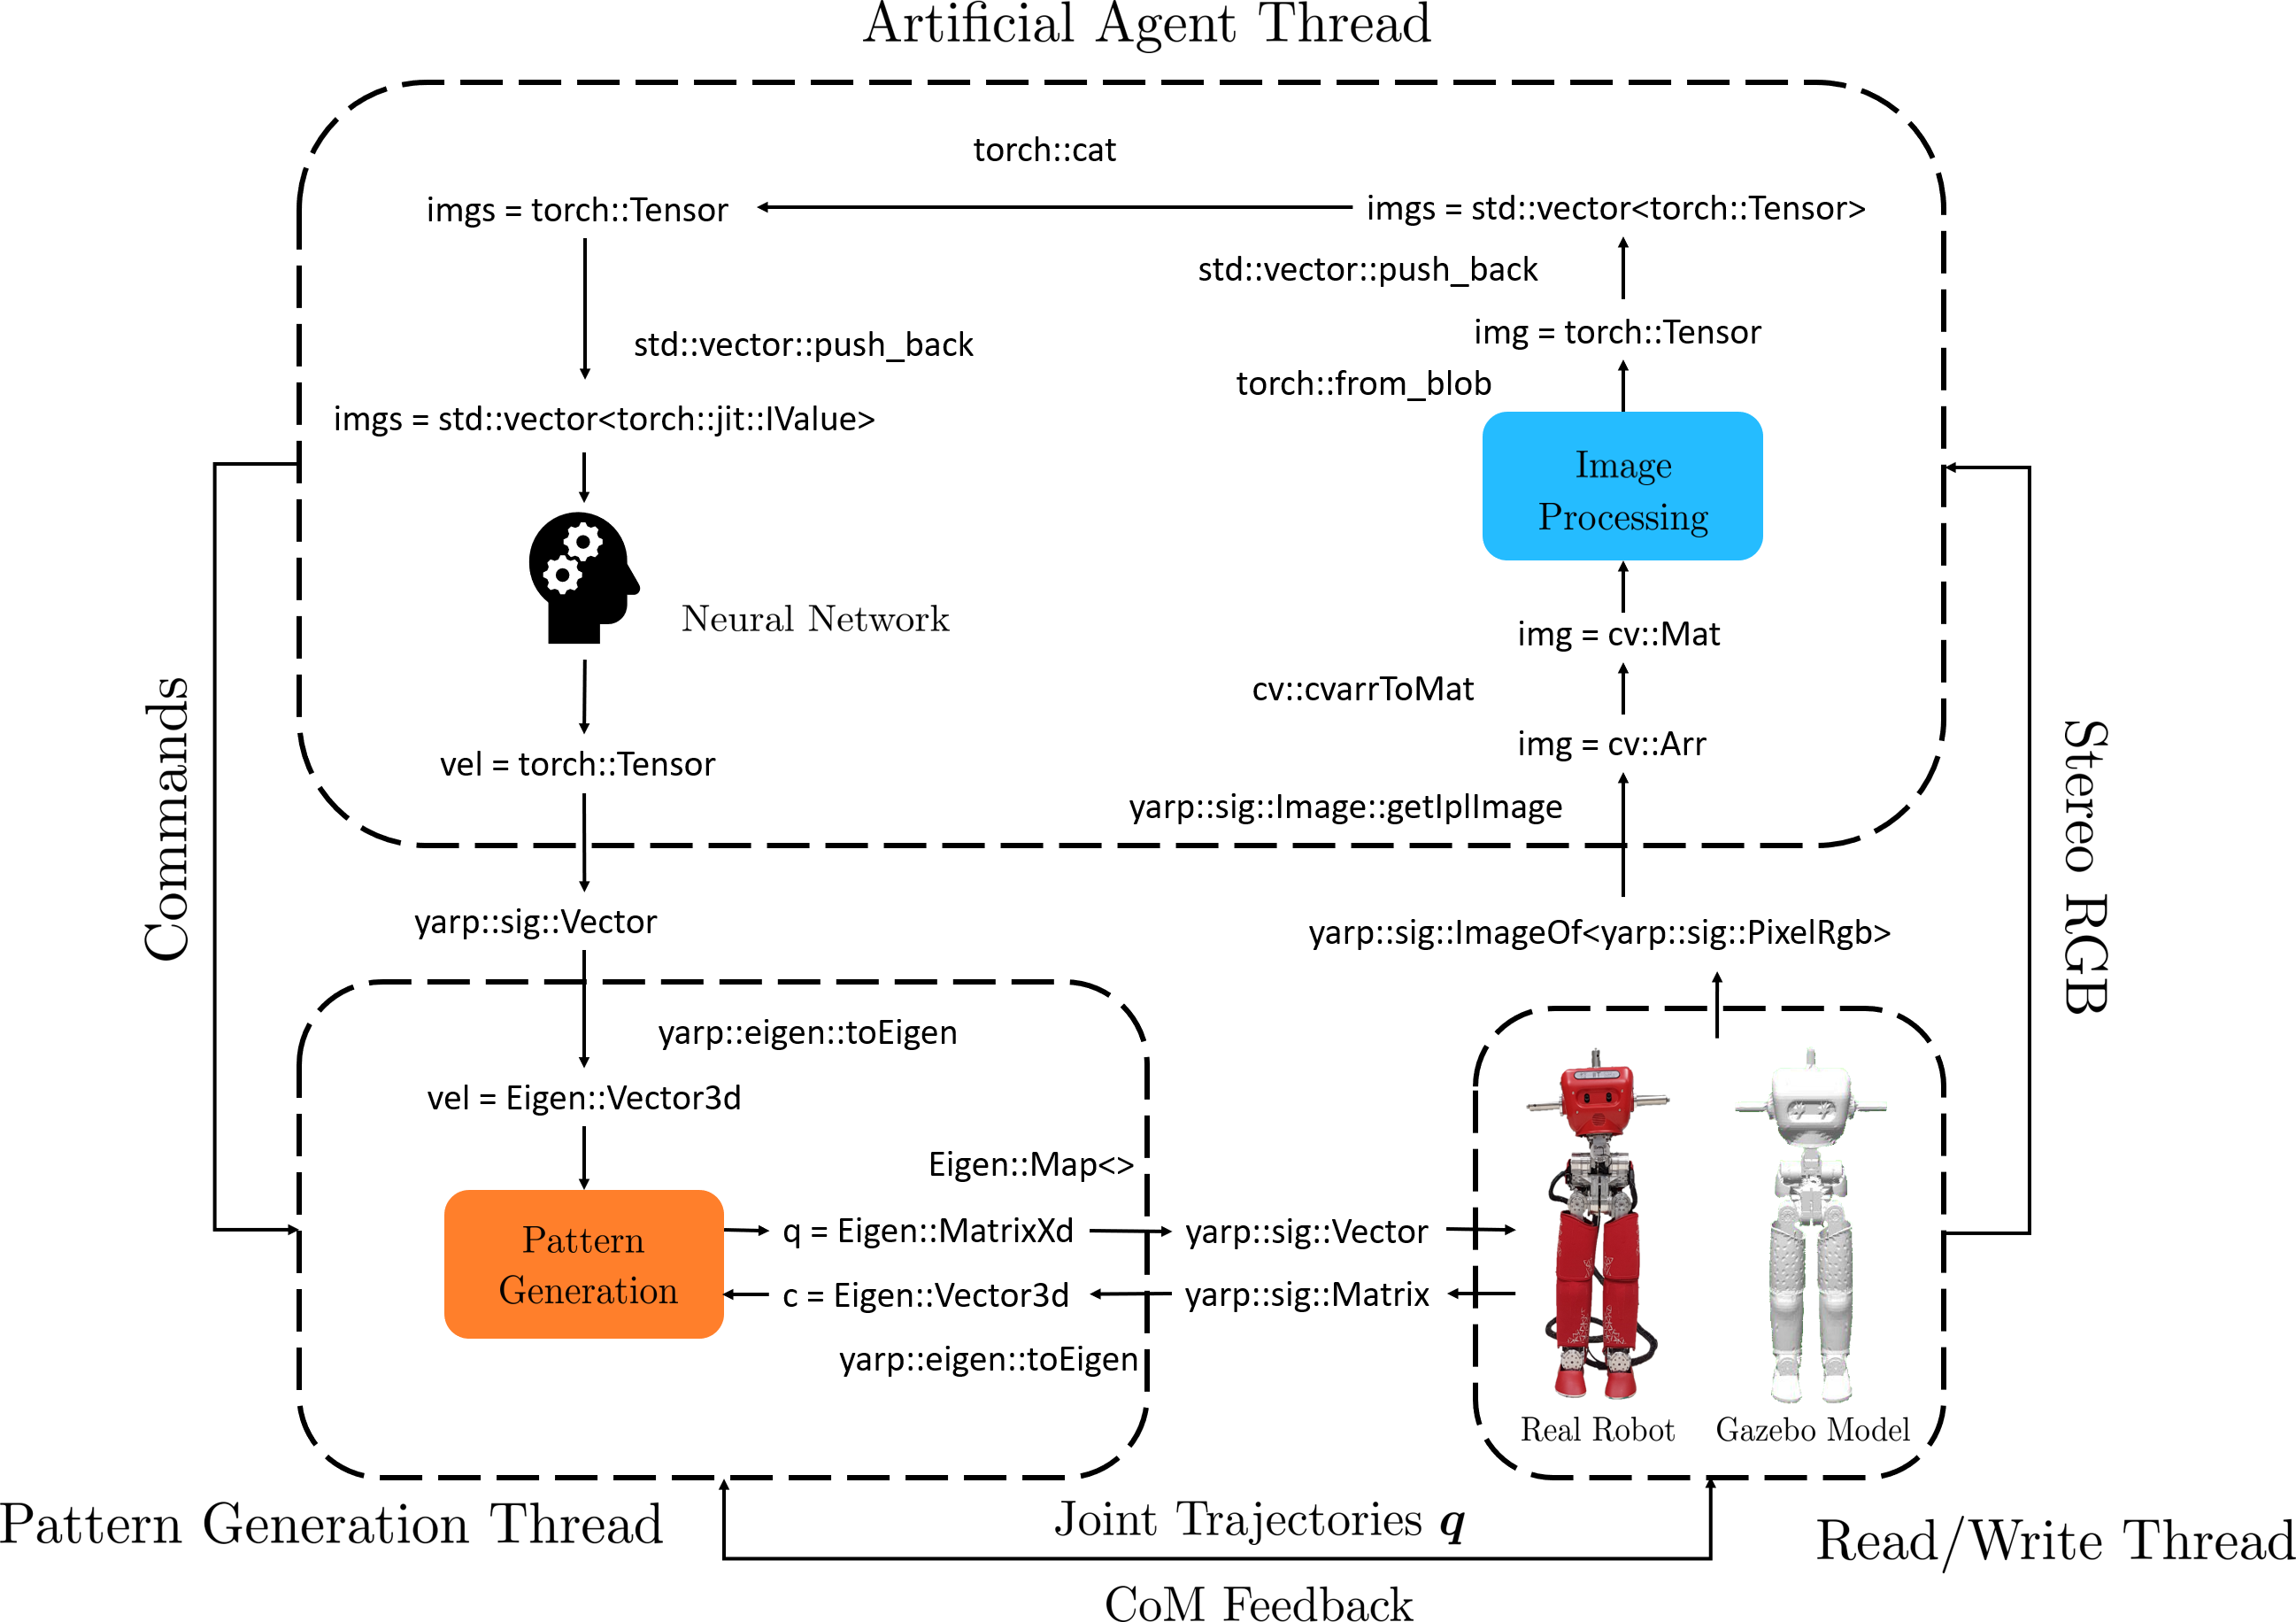
\includegraphics[scale=.4]{chapters/03_methods/img/yarp_diag.png}
	\caption{YARP is used to run multiple threads in parallel, each of which is indicated by the dashed boxes. It further enables the individual threads to communicate with each other via ports, which exchange YARP objects. It enables communication to the real robot as well as to a simulated version of it. The diagram demonstrates the types of data, which are being used, and the functions that convert them. Notice that this is an extended version of figure \ref{fig::2_cl}.}
	\label{fig::35_yarp}
\end{figure}
As we know from the previous section, one of these threads is committed to take decisions with a neural network, given RGBD images. This thread is depicted as the artificial agent thread in figure \ref{fig::35_yarp}. The pattern generation thread performs the nonlinear model predictive control, given the velocity command of the artificial agent thread. Furthermore, there are two additional running threads that communicate with Heicub's motors. These threads are the read, and the write thread in figure \ref{fig::35_yarp}. The classes, which implement the communication to the robot, are located within the io\_module folder of figure \ref{fig::31_folder}. The \inlinecode{C++}{WriteJoints} class implements a \inlinecode{C++}{yarp::os::RateThread}, which is periodically being called, to accesses the motors, which are defined within the YAML configuration file, and changes the motors' settings to position direct mode. Therefore, whatever is being written to the port that \inlinecode{C++}{WriteJoints} uses to communicate with the YARP network, and which is defined in the YAML configuration file, directly gets executed on the robot's motors. This communication to Heicub's motors corresponds to the very lowest part of figure \ref{fig::35_yarp}, where, as extensively explain in section \ref{sec::32_pg}, the pattern generation uses the forward kinematics to generate joint angles $\bm{q}$, which are being written as \inlinecode{C++}{yarp::sig::Vector} to the \inlinecode{C++}{WriteJoints} rate thread. The reading of the robot's sensors is also implemented as part of the io\_module folder in figure \ref{fig::31_folder}. There are several classes, which implement \inlinecode{C++}{yarp::os::RateThread}s for different reading tasks. Among them are the \inlinecode{C++}{ReadJoints} class, which reads out the motor encoders to obtain the joint angles, the \inlinecode{C++}{ReadCameras} class, which reads out the cameras and pushes them as \inlinecode{C++}{yarp::sig::ImageOf<yarp::sig::PixelRgb>} onto the network (see figure \ref{fig::35_yarp}), as well as the \inlinecode{C++}{AppReader} class, and the \inlinecode{C++}{KeyReader} class, which handle the communication to the joystick app, and the terminal, respectively. Both, the \inlinecode{C++}{AppReader} class, and the \inlinecode{C++}{KeyReader} class, utilize NCurses to generate a user interface on the terminal, which is internally being trapped in a while loop until exit. They readout the input, which may originate from the joystick app, or the keyboard, and push them as the velocity commands onto the YARP network (see figure \ref{fig::35_yarp} left). The velocity commands, which are converted into an \inlinecode{C++}{Eigen::Vector3d} for the \inlinecode{C++}{NMPCGenerator::SetVelocityReference} method from section \ref{sec::32_pg}, may alternatively also originate from a neural network, which is being presented in figure \ref{fig::35_yarp}. The \inlinecode{C++}{GenerateVelocityCommands} rate thread, which enables this feature, is implemented as part of the src folder in \ref{fig::31_folder}, as it only utilizes the provided libraries. It can be found at the provided \href{https://github.com/mhubii/nmpc_pattern_generator/blob/719fde0bb73925923de85cbf379c5523e075dfeb/src/behavioural_augmentation_real_robot_external_data.cpp#L108}{\underline{link}}. Its main task is to read in the images, which are constantly being pushed to the YARP network by \inlinecode{C++}{ReadCameras}, and to convert them into \inlinecode{C++}{cv::Mat} matrices, for us to perform the image processing on them, which includes the rectification, and the depth map extraction that are explained in section \ref{sec::224_ip}. The \inlinecode{C++}{GenerateVelocityCommands} class additionally stores a sequence of the processed images in the form of a \inlinecode{C++}{std::vector<torch::Tensor>}. Whenever a new image is read from the YARP network, the oldest image within the \inlinecode{C++}{std::vector<torch::Tensor>} is being deleted, and all other images are shifted up by one index, such that the newest image is available as the first entry. This vector of tensors is then being converted into a single tensor, by concatenating the individual tensors along the first dimension, which is, by definition of the long short term memory units, required in PyTorch. The concatenated tensor is further being converted into a \inlinecode{C++}{std::vector<torch::jit::IValue>}, such that the JIT script, which defines the neural network that got trained in Python (see \ref{sec::33_dl}), can forward it. The output is then obtained as a \inlinecode{C++}{torch::Tensor} yet again, which is being written in the form of a \inlinecode{C++}{yarp::sig::Vector} to the YARP network, such that,  as explained above, the pattern generation can use it as input. This pipeline works equivalently on the real robot, as well as on a simulated version of it in Gazebo \cite{koenig2004design}, for which install instructions are provided in the appendix \ref{sec::A4_sm}. Although it allowed us to prototype within the simulation, we will use the pipeline to train the real robot Heicub, as an example for our method, on finding a fire extinguisher within the next section - Experiments.


	
	\chapter{Experiments}
	\label{sec::4_ex}
Within the experiments chapter, we will first benchmark the nonlinear model predictive control implementation of ours for purely simulated tasks in section \ref{sec::41_uc}, and then tune hyperparameters for it to run well on Heicub. This will allow us to define a standardized environment for walking experiments in section \ref{sec::412_pt}, to later compare user-controlled performance against autonomously controlled performance in section \ref{sec::42_aw}. Though, before we can tackle the idea of behavioral cloning, which got described in section \ref{sec::222_bc}, we need to meet the prerequisites, that is we will calibrate the camera, and tune the depth map parameter extraction in sections \ref{sec::421_cc}, and \ref{sec::422_dp}, respectively. All of the above-mentioned steps, will then allow us to collect data and to train a newly developed neural network architecture on it in section \ref{sec::423_da}. Finally, we will compare the humanly controlled robot's balance with the artificially controlled robot's balance in section \ref{sec::424_pt} and investigate on the reinforcement learning approach for autonomous navigation in section \ref{sec::425_pp}.
	\FloatBarrier
\section{User-Controlled Walking}
\label{sec::41_uc}
As the fundamental building block for the comparison to autonomous walking, we now need to investigate on user-controlled walking. This enables us, in contrast to the control by a neural network, to find the best parameters for the pattern generation in a well controllable environment. These parameters will then be kept constant throughout the rest of this thesis, in order to allow for a good comparison between user-controlled walking and autonomously controlled walking. Furthermore, we will rely on them to gather data for the behavioral cloning approach in section \ref{sec::423_da}.
\FloatBarrier
\subsection{Benchmarking of Implementation}
\label{sec::411_bm}
To evaluate the pattern generator implementation of ours, we have benchmarked it against an existing one, which was written in Python. Therefore, we defined velocity commands, as they typically may appear in real-world scenarios. The four defined use cases, which are shown in figures \ref{fig::411_benchmarking_basic} and \ref{fig::411_benchmarking_advanced}, were parametrized in accordance to the HRP-2 humanoid robot.
\begin{figure}[h!]
	\centering
	\subcaptionbox{Straight trajectories at\\$\bm{v}=\begin{pmatrix}
		0.1 & 0.0 & 0.0
		\end{pmatrix}^T$.}%
	[.45\linewidth]{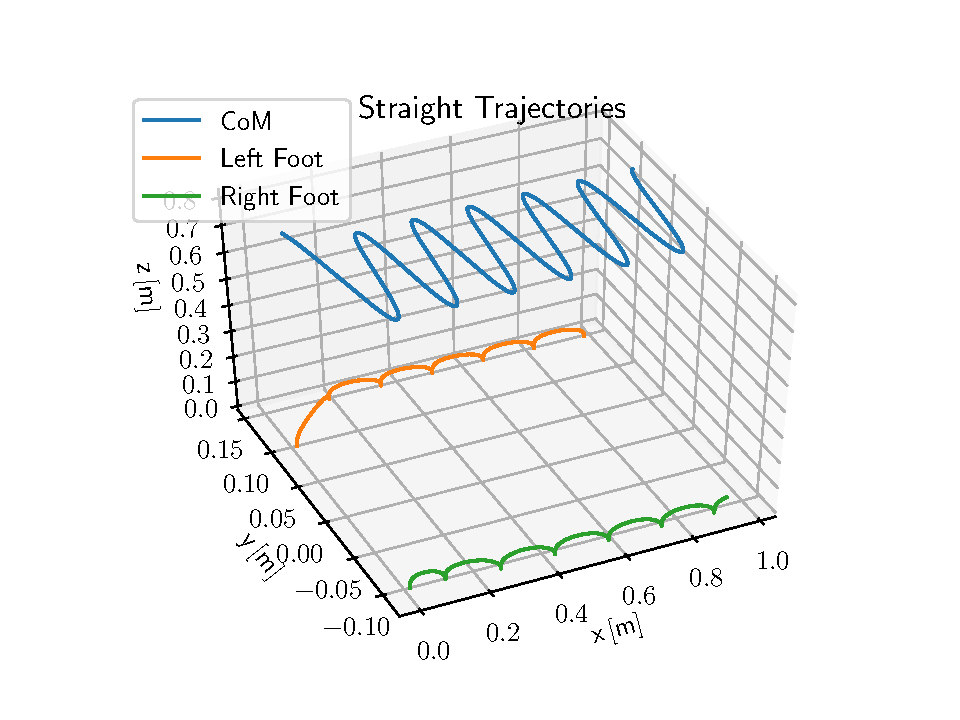
\includegraphics[scale=.45]{chapters/04_experiments/01_user_controlled_walking/01_benchmarking/nmpc_straight.pdf}}
	\subcaptionbox{Diagonal trajectories at\\$\bm{v}=\begin{pmatrix}
		0.1 & 0.1 & 0.0
		\end{pmatrix}^T$.}%
	[.45\linewidth]{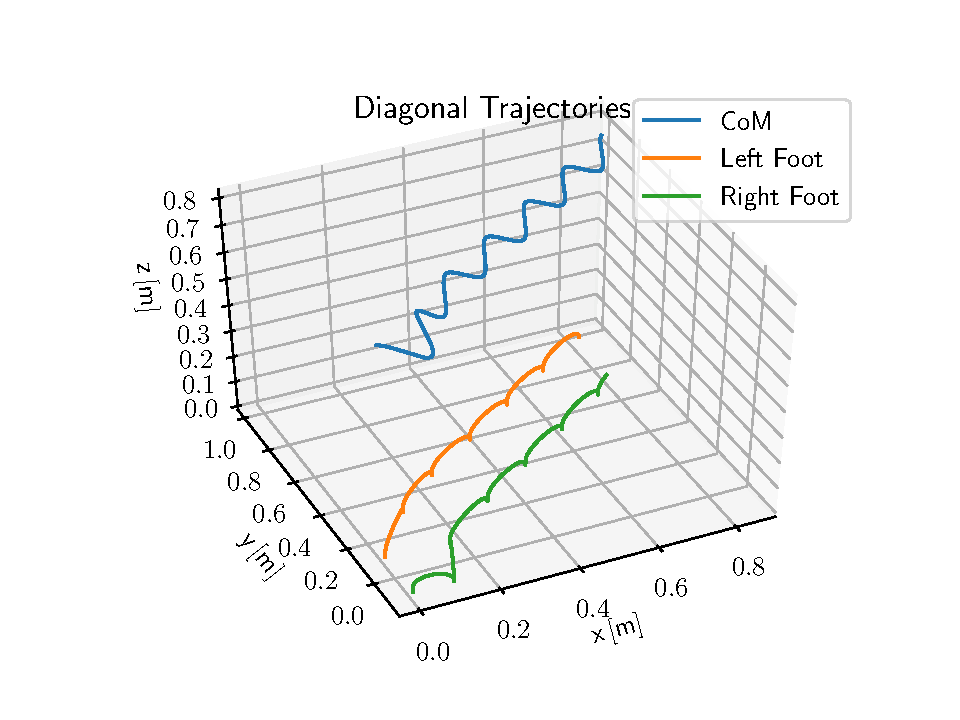
\includegraphics[scale=.45]{chapters/04_experiments/01_user_controlled_walking/01_benchmarking/nmpc_diagonal.pdf}}
	\caption{Simple trajectories. The velocities are given in units of\\$(\text{m}/\text{s}\,\,\,\,\text{m}/\text{s}\,\,\,\,\text{rad}/\text{s})^T$, where the first two entries describe the robot's velocity in the x-, and the y-direction, and the last entry describes the robot's angular velocity about the z-axis, form a frame that is attached to the robot. The trajectories start on the left-hand side.}
	\label{fig::411_benchmarking_basic}
\end{figure} 
The parameters for these tests can be found in the YAML file at the provided \href{https://github.com/mhubii/nmpc_pattern_generator/blob/719fde0bb73925923de85cbf379c5523e075dfeb/libs/pattern_generator/configs_hrp2.yaml#L1}{\underline{link}}. To obtain the pattern generator's performance, in terms of speed, the straight walk experiment in figure \ref{fig::411_benchmarking_basic} (a) got executed ten times on an Intel Core i7-7700HQ CPU at $2.8\,\text{GHz}$, for both, the Python and our implementation. It took $873\pm23\,\text{ms}$ and $147.7\pm0.5\,\text{ms}$ to execute the code for $100$ iterations on average, which means that a single iteration took $8.73\pm0.23\,\text{ms}$ and $1.48\pm0.01\,\text{ms}$. It was therefore possible to achieve a speedup of around $600$ percent with the presented implementation. We further demonstrate the avoidance of a convex obstacle with a security margin that keeps the robot at a safe distance in figure \ref{fig::411_benchmarking_advanced} (b). The used obstacle is defined to be located at $x=1.6\,\text{m}$ and $y=1.0\,\text{m}$, with a radius of $R=1.0\,\text{m}$, and a security margin of $m=0.4\,\text{m}$.
\begin{figure}[h!]
	\centering
	\subcaptionbox{Curved trajectories at\\$\bm{v}=\begin{pmatrix}
	0.1 & 0.0 & 0.1
	\end{pmatrix}^T$.}%
	[.45\linewidth]{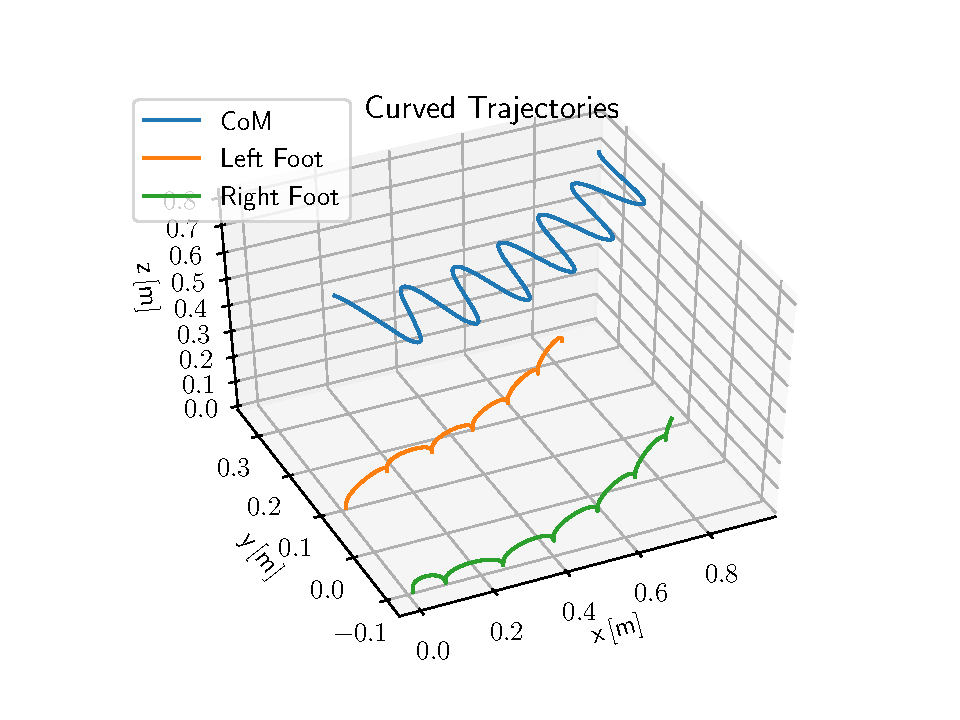
\includegraphics[scale=.45]{chapters/04_experiments/01_user_controlled_walking/01_benchmarking/nmpc_turn.pdf}}
	\subcaptionbox{Obstacle avoidance at\\$\bm{v}=\begin{pmatrix}
	0.1 & 0.0 & 0.0
	\end{pmatrix}^T$}%
	[.45\linewidth]{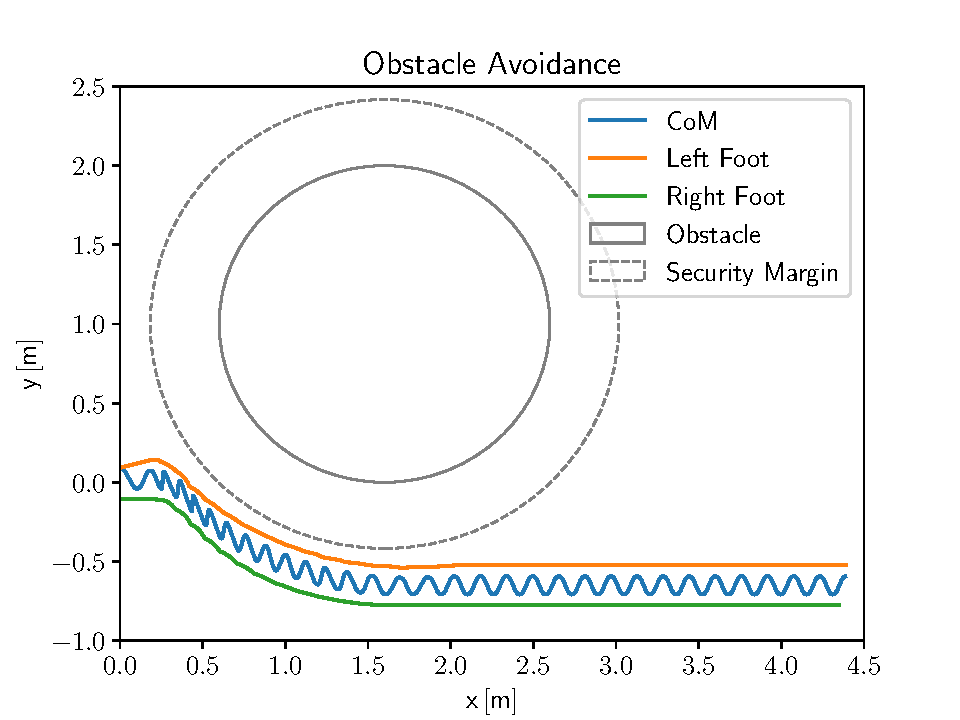
\includegraphics[scale=.45]{chapters/04_experiments/01_user_controlled_walking/01_benchmarking/nmpc_obstacle.pdf}}
	\caption{Advanced trajectories. The velocities are given in units of\\$(\text{m}/\text{s}\,\,\,\,\text{m}/\text{s}\,\,\,\,\text{rad}/\text{s})^T$, see figure \ref{fig::411_benchmarking_basic}.}
	\label{fig::411_benchmarking_advanced}
\end{figure} 
To always ensure a smooth motion, and to benchmark the interpolation, we plotted the x-, y-, and z-trajectories for the left and the right foot, as shown in figure \ref{fig::411_benchmarking_inter}. The plots were generated on the curved trajectory of figure \ref{fig::411_benchmarking_advanced} (a), and they reveal a continuous behavior at every time step for all dimensions.
\begin{figure}[h!]
	\centering
	\subcaptionbox{Interpolated\\x-Trajectories}%
	[.3\linewidth]{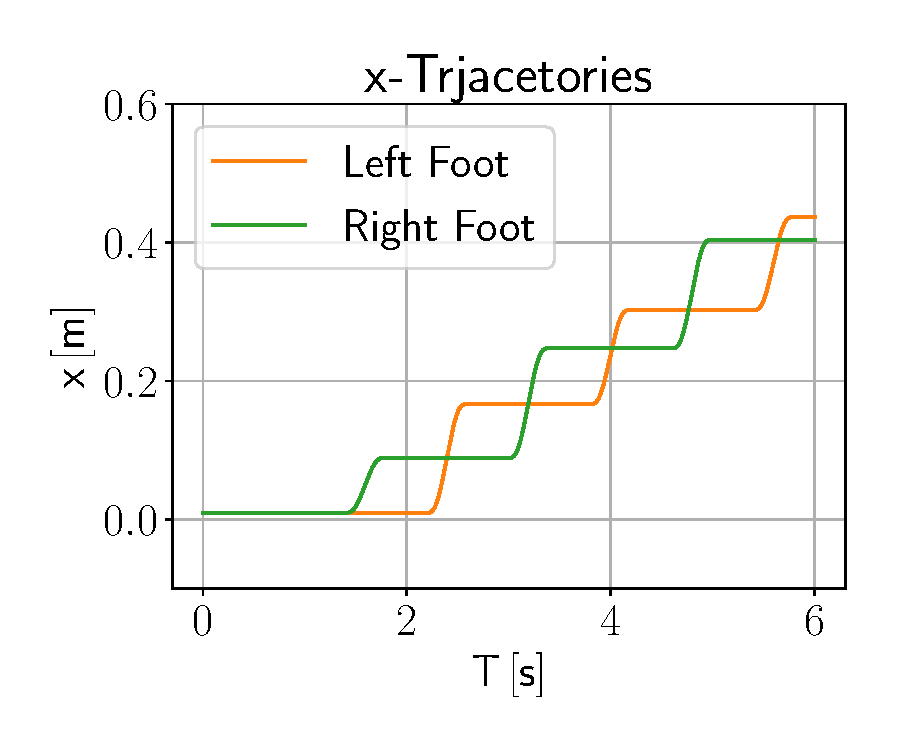
\includegraphics[scale=.3]{chapters/04_experiments/01_user_controlled_walking/01_benchmarking/interpolated_x_trajectories.pdf}}
	\subcaptionbox{Interpolated\\y-Trajectories}%
	[.3\linewidth]{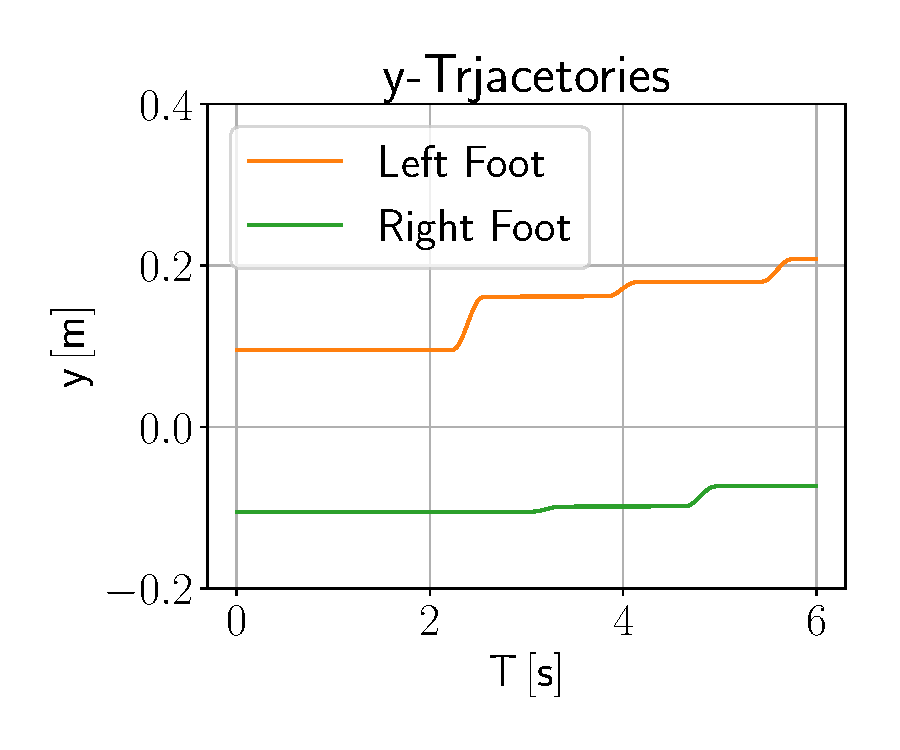
\includegraphics[scale=.3]{chapters/04_experiments/01_user_controlled_walking/01_benchmarking/interpolated_y_trajectories.pdf}}
	\subcaptionbox{Interpolated\\z-Trajectories}%
	[.3\linewidth]{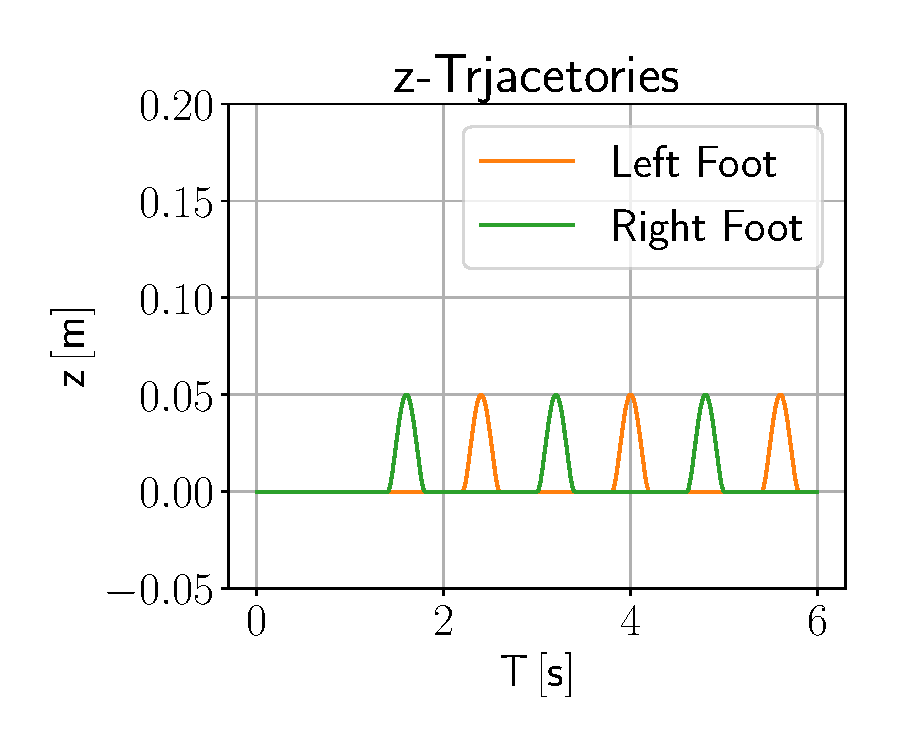
\includegraphics[scale=.3]{chapters/04_experiments/01_user_controlled_walking/01_benchmarking/interpolated_z_trajectories.pdf}}
	\caption{Interpolated foot trajectories. As explained in figure \ref{fig::213_ip}, the interpolation interpolates the feet's movement, given an initial, and a final foot position. The continuity shows that the interpolation got implemented correctly.}
	\label{fig::411_benchmarking_inter}
\end{figure}
 The benchmarked pattern generator then enabled us to run it on the real robot, which we did in a test environment that will be presented in the next section - Performance in Test Environment.
\FloatBarrier
\subsection{Performance in Test Environment}
\label{sec::412_pt}
For the execution on Heicub, we chose a parameter setting with which we could ensure balanced motion for all velocity commands. This could be achieved by choosing the parameters, which are listed in the YAML configurations file at the provided \href{https://github.com/mhubii/nmpc_pattern_generator/blob/719fde0bb73925923de85cbf379c5523e075dfeb/libs/pattern_generator/configs.yaml#L1}{\underline{link}}. The most important ones therein are further shown in table \ref{tab::412_params}.
\begin{table}
	\centering
	\caption{Parameters which used to work best on Heicub.}
	\begin{tabular}{lclc}
		Parameter&Value&Parameter&Value\\
		\hline
		$T_{\text{Step}}$ & $3.20\,\text{s}$ & $N$ & $16\,\text{\#}$ \\
		$T_{\text{Double Support}}$ & $1.60\,\text{s}$ & $\alpha$ & $1.0\,\text{a.u.}$ \\
		$T_{\text{Command Period}}$  & $0.01\,\text{s}$& $\beta$ & $100\,\text{a.u.}$ \\
		$T_{\text{Preview}}$ & $0.40\,\text{s}$ & $\gamma$ & $0.01\,\text{a.u.}$
	\end{tabular}
	\label{tab::412_params}
\end{table}
Now given these parameters, we designed an environment for Heicub to walk in. A human user had to control the robot in four different scenarios. In each of the scenarios, Heicub started from a reference position, in order to reach a fire extinguisher at a distant location. By design, the setup allows for benchmarking of dynamic balance in all four different scenarios. As will be shown in section \ref{sec::42_aw}, we require a neural network to execute the same tasks, and therefore we can compare the performances of a human user with that of an autonomous agent. For the dynamic balance evaluation, we extracted the desired ZMP from the nonlinear model predictive controller, and measured the true ZMP, in accordance to equations \ref{eq::211_double_zmp_x} and \ref{eq::211_double_zmp_y}, by recording the ankles' force-torque sensor readouts. We further kept track of the velocity commands to the pattern generator for all tasks to extract the user's behavior. The first task was simply to go two meters straight forward (figure \ref{fig::412_uc_straight}).
\begin{figure}[h!]
	\subcaptionbox{Dynamic balance.}%
	[.5\linewidth]{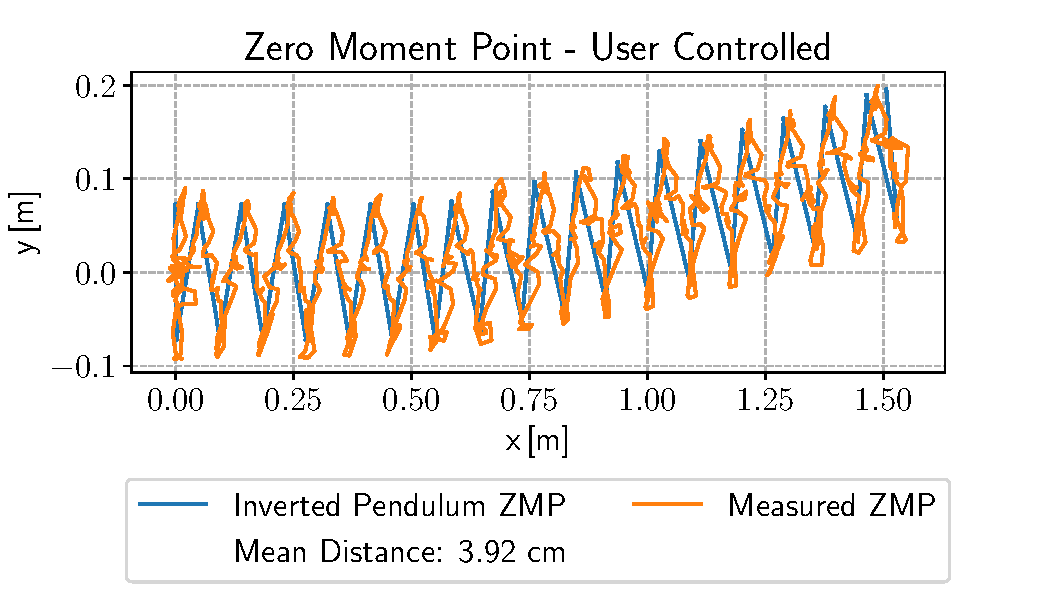
\includegraphics[scale=.45]{chapters/04_experiments/01_user_controlled_walking/02_test_environment/straight_walk_01_zmp.pdf}}
	\subcaptionbox{Behavior.}%
	[.5\linewidth]{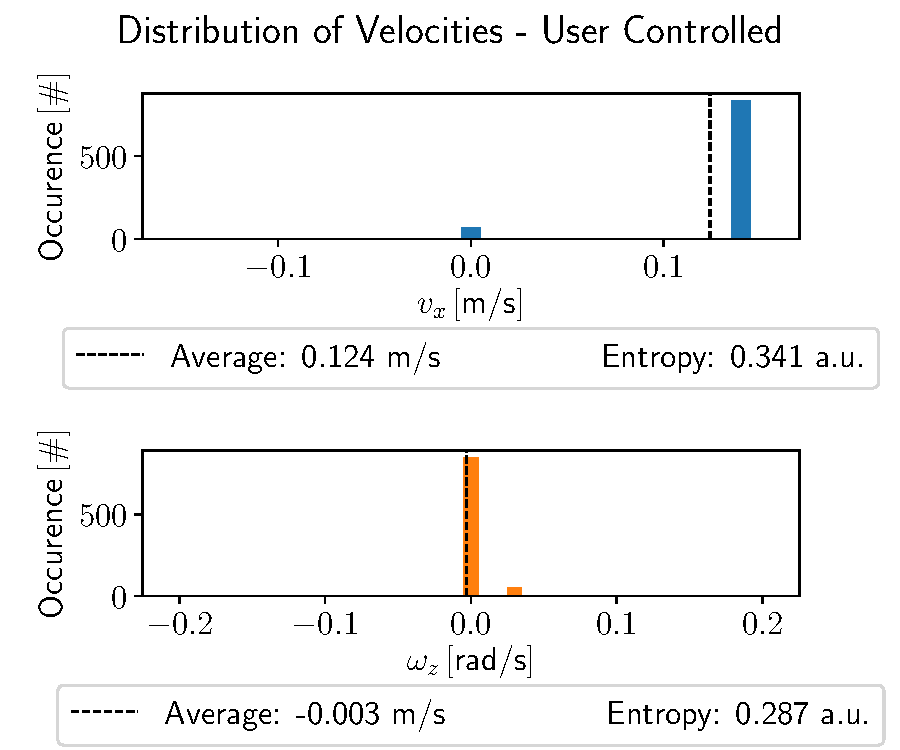
\includegraphics[scale=.45]{chapters/04_experiments/01_user_controlled_walking/02_test_environment/straight_walk_01_entropy.pdf}}
	\caption{User-controlled straight walk. The robot started to the plot's left-hand side (a), and moved forward until it reached the fire extinguisher.}
	\label{fig::412_uc_straight}
\end{figure} 
The behavior therein is visualized by a histogram of all velocity commands over the course of the task (figure \ref{fig::412_uc_straight} (b)). For the bin size we chose $0.01\,\text{m}/\text{s}$ and $0.01\,\text{rad}/\text{s}$, respectively. 
\begin{figure}[h!]
	\subcaptionbox{Dynamic balance.}%
	[.5\linewidth]{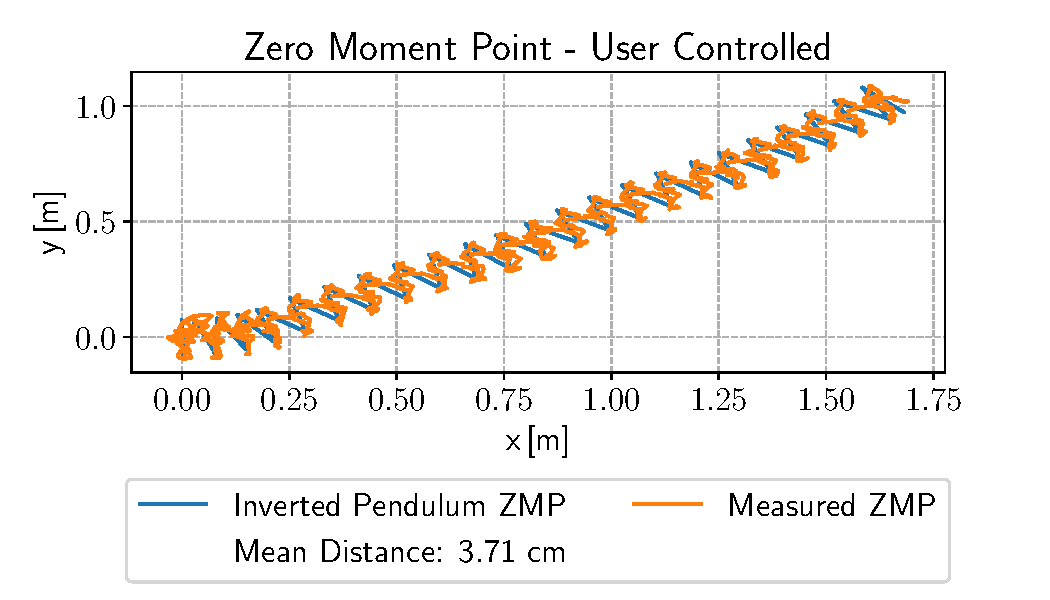
\includegraphics[scale=.45]{chapters/04_experiments/01_user_controlled_walking/02_test_environment/curved_walk_01_zmp.pdf}}
	\subcaptionbox{Behavior.}%
	[.5\linewidth]{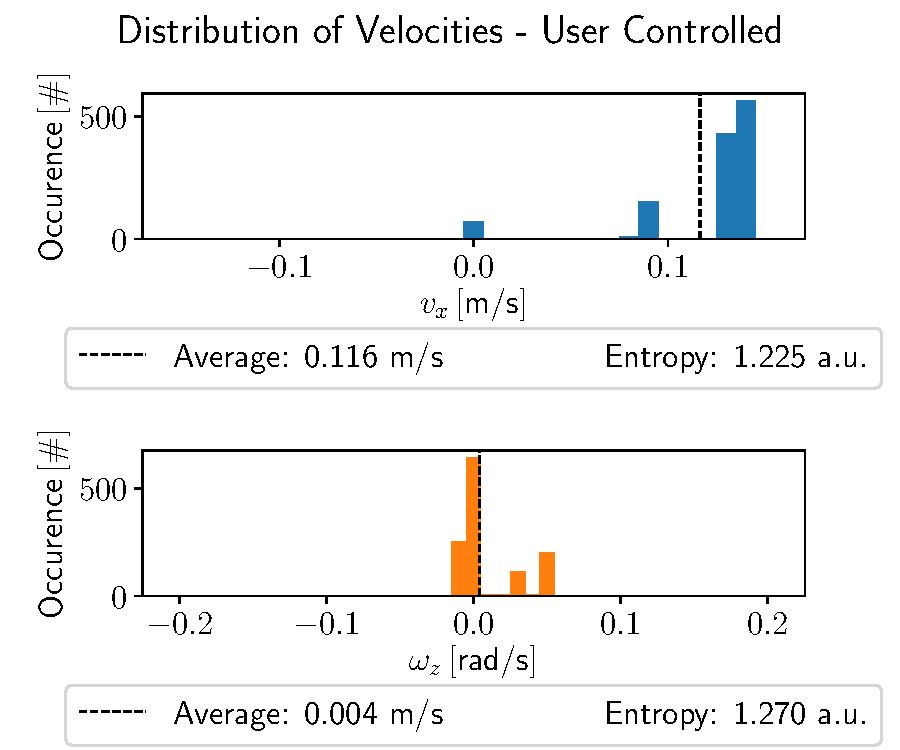
\includegraphics[scale=.45]{chapters/04_experiments/01_user_controlled_walking/02_test_environment/curved_walk_01_entropy.pdf}}
	\caption{User-controlled curved walk. The robot started to the plot's left-hand side (a), and performed a left turn on its way to the fire extinguisher, where it stopped.}
	\label{fig::412_uc_curved}
\end{figure} 
The second task was to reach the fire extinguisher, which was located to the left of the robot. In order to reach it, it was therefore required to perform a curved walk (figure \ref{fig::412_uc_curved}). The third task (figure \ref{fig::412_uc_obstacle}) involved the avoidance of an obstacle, namely a chair. For the fourth task (figure \ref{fig::412_uc_sight}), the robot started with its back pointing towards the fire extinguisher.
\begin{figure}[h!]
	\subcaptionbox{Dynamic balance.}%
	[.5\linewidth]{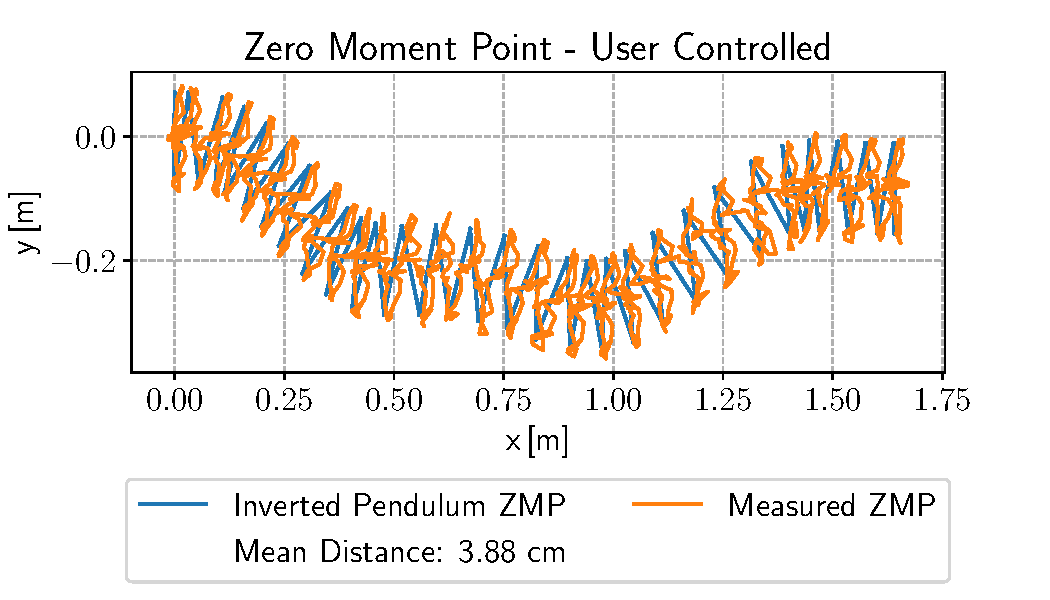
\includegraphics[scale=.45]{chapters/04_experiments/01_user_controlled_walking/02_test_environment/obstacle_walk_02_zmp.pdf}}
	\subcaptionbox{Behavior.}%
	[.5\linewidth]{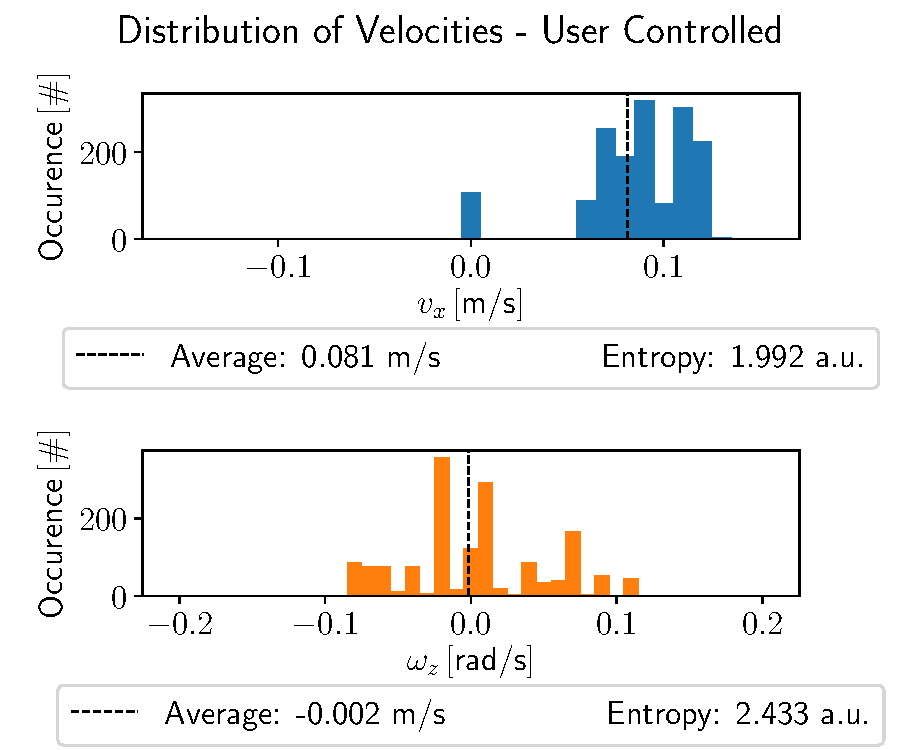
\includegraphics[scale=.45]{chapters/04_experiments/01_user_controlled_walking/02_test_environment/obstacle_walk_02_entropy.pdf}}
	\caption{User-controlled obstacle avoidance. The robot started to the plot's left-hand side (a), and moved towards a fire extinguisher. On about half of the distance it avoided a chair by turning to the right, and then to the left again, until it reached the fire extinguisher and stopped.}
	\label{fig::412_uc_obstacle}
\end{figure} 
\begin{figure}[h!]
	\subcaptionbox{Dynamic balance.}%
	[.5\linewidth]{\includegraphics[scale=.45]{chapters/04_experiments/01_user_controlled_walking/02_test_environment/out_of_sight_walk_01_zmp.pdf}}
	\subcaptionbox{Behavior.}%
	[.5\linewidth]{\includegraphics[scale=.45]{chapters/04_experiments/01_user_controlled_walking/02_test_environment/out_of_sight_walk_01_entropy.pdf}}
	\caption{User-controlled environmental scanning. The robot started to the plot's right-hand side (a), facing to the right, and performed a full $180^\circ$ turn, before walking almost straight to the fire extinguisher, which is here located to the plot's left-hand side.}
	\label{fig::412_uc_sight}
\end{figure} 
\newpage
	\FloatBarrier
\section{Autonomous Walking}
\label{sec::42_aw}
The autonomous walking is based upon the performance within the test environment from section \ref{sec::412_pt}. The found parameters are used for comparative reason throughout this section as well. As explained in section \ref{sec::224_ip}, the neural network benefits strongly from an available depth map as input. We will therefore deal with the depth map extraction first.
\FloatBarrier
\subsection{Camera Calibration}
\label{sec::421_cc}
As described in section \ref{sec::224_ip}, in order for the stereo block matching algorithm to work properly (equation \ref{eq::224_sad}), it is required to calibrate the cameras. We shortly verified this in figure \ref{fig::421_no_calib}, where we extracted a depth map from the uncalibrated stereo camera pair.
\begin{figure}[h!]
	\centering
	\subcaptionbox{Left disparity map.}%
	[.4\linewidth]{\includegraphics[scale=.3]{chapters/04_experiments/02_autonomous_walking/02_depth_map_parameter_tuning/disp_no_calib.png}}
	\subcaptionbox{Confidence weighted least squares filtered disparity map.}%
	[.4\linewidth]{\includegraphics[scale=.3]{chapters/04_experiments/02_autonomous_walking/02_depth_map_parameter_tuning/wls_no_calib.png}}
	\caption{Depth map extraction without calibration. The parameters were set as follows to $N=13$, $D=32$, $\sigma = 1$, and $\lambda=10^4$.}
	\label{fig::421_no_calib}
\end{figure}
For the calibration we chose to use a chess-board calibration pattern, see figure \ref{fig::421_calib}. The used calibration pattern has width of $W=8$, and a height of $H=6$, where each square has a size of $a=22.5\,\text{mm}$ (equation \ref{eq::224_square_size}). We took a total of $N=60$ images of the calibration pattern for varying orientations and translations with respect to the camera, which results in a total of $W\times H\times N = 2880$ points for the calibration. 
\begin{figure}[h!]
	\centering
	\includegraphics[scale=.28]{chapters/04_experiments/02_autonomous_walking/01_camera_calibration/calib.png}
	\caption{Exemplary left and right camera views of the calibration pattern as acquired during the calibration process. The colorful points indicate the detected corners in the image plane. Refer to figure \ref{fig::224_distortion} for the theory.}
	\label{fig::421_calib}
\end{figure}
As the resulting mean squared re-projection error $\Delta \bar{x} = 1/(WHN)\sum_0^{WHN} \Delta x$ (equation \ref{eq::224_reprojection}), we obtained $\Delta \bar{x}_l = 0.26\, \text{pixel}$, and $\Delta \bar{x}_r = 0.25\,\text{pixel}$, for the left, and the right camera, respectively. According to equations \ref{eq::224_focal_intrinsics}, \ref{eq::224_x_dist}, and \ref{eq::224_y_dist}, we therefore determined the camera's intrinsic parameters as listed in table \ref{tab::421_intrinsics}.
\begin{table}
	\centering
	\caption{Intrinsic parameters of single cameras. These parameters can be found as YAML file on GitHub (\href{https://github.com/mhubii/nmpc_pattern_generator/tree/master/libs/io_module}{\underline{link}}).\label{tab::421_intrinsics}}
	\begin{tabular}{lll}
		Intrinsic Parameter & Left Camera & Right Camera\\
		\hline
		$f_x\,[\text{pixel}/\text{mm}]$ & $\quad2.36\cdot10^2$ & $\quad2.32\cdot10^2$ \\
		$f_y\,[\text{pixel}/\text{mm}]$ & $\quad2.37\cdot10^2$ & $\quad2.32\cdot10^2$ \\
		$c_x\,[\text{pixel}]$ & $\quad1.63\cdot10^2$ & $\quad1.86\cdot10^2$ \\
		$c_y\,[\text{pixel}]$ & $\quad1.11\cdot10^2$ & $\quad1.30\cdot10^2$ \\
		$k_1\,[1/\text{pixel}^2]$ & $-4.54\cdot10^{-1}$ & $-4.58\cdot10^{-1}$ \\
		$k_2\,[1/\text{pixel}^4]$ & $\quad2.90\cdot10^{-1}$  & $\quad3.18\cdot10^{-1}$  \\
		$k_3\,[1/\text{pixel}^6]$ & $-1.21\cdot10^{-1}$ & $-1.48\cdot10^{-1}$ \\
		$p_1\,[1/\text{pixel}]$ & $-2.73\cdot10^{-3}$ & $\quad3.02\cdot10^{-4}$  \\
		$p_2\,[1/\text{pixel}]$ & $\quad2.16\cdot10^{-4}$  & $\quad7.63\cdot10^{-4}$		
	\end{tabular}
\end{table}
Then given the calibration of each single camera, for each camera we computed the rectification transforms $\bm{R}_i$, and the projection matrices $\bm{P}_i$ in the rectified coordinate system, all of which can be found in table \ref{tab::421_extrinsics}.
\begin{table}
	\centering
	\caption{Rectification transforms $\bm{R}_i$, and projection matrices $\bm{P}_i$, for the left, and the right camera, respectively. These parameters can be found as YAML file on GitHub (\href{https://github.com/mhubii/nmpc_pattern_generator/blob/master/libs/io_module/cam_stereo.yaml}{\underline{link}}). \label{tab::421_extrinsics}}
	\begin{tabular}{lll}
		Camera & Extrinsic Parameter & \\ 
		\hline
		&& \\
		\multirow{5}{*}{Left} & $\bm{R}\,[\text{a.u.}]$              & $\begin{pmatrix}
		\quad9.93\cdot10^{-1} & -2.65\cdot10^{-3}     & \quad1.14\cdot10^{-1} \\ 
		\quad5.41\cdot10^{-1} & \quad1.00\cdot10^{0}  & -2.39\cdot10^{-2} \\
		-1.14\cdot10^{-1}     & \quad2.43\cdot10^{-2} & \quad9.93\cdot10^{-1}
		\end{pmatrix}$ \\&&\\
		& $\bm{P}\,[\text{pixel}/\text{mm}]$              & $\begin{pmatrix}
		2.34\cdot10^{2} & 0.00     & 1.88\cdot10^{2} & 0.00\,\text{mm} \\ 
		0.00 & 2.34\cdot10^{2}  & 4.87\cdot10^{1} & 0.00\,\text{mm} \\
		0.00    & 0.00 & 1.00 & 0.00\,\text{mm}
		\end{pmatrix}$ \\
		&&\\
		\multirow{5}{*}{Right} & $\bm{R}\,[\text{a.u.}]$              & $\begin{pmatrix}
		\quad9.95\cdot10^{-1} & -2.30\cdot10^{-2}     & \quad9.93\cdot10^{-2} \\ 
		\quad2.07\cdot10^{-2} & \quad1.00\cdot10^{0}  & \quad2.38\cdot10^{-2} \\
		-9.98\cdot10^{-2}     & -2.16\cdot10^{-2} & \quad9.95\cdot10^{-1}
		\end{pmatrix}$ \\&&\\
		& $\bm{P}\,[\text{pixel}/\text{mm}]$              & $\begin{pmatrix}
		2.34\cdot10^{2} & 0.00     & 1.88\cdot10^{2} & -1.60\cdot10^1\,\text{mm} \\ 
		0.00 & 2.34\cdot10^{2}  & 4.88\cdot10^{1} & 0.00\,\text{mm} \\
		0.00    & 0.00 & 1.00 & 0.00\,\text{mm}
		\end{pmatrix}$ \\
	\end{tabular}
\end{table}
Exemplary rectified images, which rely on the matrices of table \ref{tab::421_extrinsics}, are shown in figure \ref{fig::421_rect} (a). Since there is a slight rotation of the calibration pattern, it is not obvious that the images got rectified well. Therefore, the same images are shown in figure \ref{fig::421_rect} (b), but slightly rotated such that the calibration pattern aligns horizontally. The blue line therein indicates that in contrast to the original image, straight lines now appear straight across both images, which is crucial for the block matching algorithm in the next section - Depth Map Parameter Tuning.
\begin{figure}[h!]
	\centering
	\subcaptionbox{Rectified images.}%
	[.4\linewidth]{\includegraphics[scale=.25]{chapters/04_experiments/02_autonomous_walking/01_camera_calibration/rect.png}}
	\subcaptionbox{Rotated rectified images.}%
	[.4\linewidth]{\includegraphics[scale=.25]{chapters/04_experiments/02_autonomous_walking/01_camera_calibration/rect_line.png}}
	\caption{Rectified and original view of the stereo camera. Refer to figure \ref{fig::224_rectified} for the theory.}
	\label{fig::421_rect}
\end{figure}
\FloatBarrier
\subsection{Depth Parameter Tuning}
\label{sec::422_dp}
Within this section, we shortly explore the effects of all tunable parameters on the depth map generation. Therefore, we utilize a simple experimental setup. Within the setup, Heicub points its stereo camera towards three chairs that are located at a distance of $1\,\text{m}$ towards each other, and towards the cameras, so to cover close, medium, and far distances. The consecutive chairs are slightly shifted, in order to enable the simultaneous observation of all of them. The rectified view of the environment is shown in figure \ref{fig::422_wls_rgb}.
\begin{figure}[h!]
	\centering
	\subcaptionbox{Left camera's view.}%
	[.4\linewidth]{\includegraphics[scale=.3]{chapters/04_experiments/02_autonomous_walking/02_depth_map_parameter_tuning/l_rgb.png}}
	\subcaptionbox{Right camera's view.}%
	[.4\linewidth]{\includegraphics[scale=.3]{chapters/04_experiments/02_autonomous_walking/02_depth_map_parameter_tuning/r_rgb.png}}
	\caption{Heicub's perspective of the scene for the depth map parameter tuning.}
	\label{fig::422_wls_rgb}
\end{figure}
The depth map extraction, which utilizes the rectified images, depends on a stereo block matching algorithm that was explained in section \ref{sec::224_ip}. It mainly depends on the window size and the number of disparities for the sum of absolute difference computation. We evaluate the influence of those two parameters in figure \ref{fig::422_disp} (a) in a grid search fashion. It is apparent that the change in the number of disparities has close to no influence onto the depth map quality, while it removes plenty of useful information from the left hand side of images. The same holds true for the window size, except that it removes some noise from the depth maps.
\begin{figure}[h!]
	\centering
	\subcaptionbox{Left disparity. Please refer to figure \ref{fig::224_left_disparity_map} and equation \ref{eq::224_sad} for the theory.}%
	[.45\linewidth]{\includegraphics[scale=.2]{chapters/04_experiments/02_autonomous_walking/02_depth_map_parameter_tuning/disp_sad.png}}
	\subcaptionbox{Confidence weighted least squares disparity map. Please refer to figure \ref{fig::224_weighted_least_squares_disparity} and equation \ref{eq::224_wls_final} for the theory.}%
	[.45\linewidth]{\includegraphics[scale=.2]{chapters/04_experiments/02_autonomous_walking/02_depth_map_parameter_tuning/disp_sad_wls.png}}
	\caption{Left disparity map and confidence weighted least squares disparity for changing SAD window sizes $N$ and number of disparities $D$.}
	\label{fig::422_disp}
\end{figure}
In combination with the confidence weighted least squares filtering, we can observe that most of the noise is already removed (figure \ref{fig::422_disp} (b)), for which it is more import to keep the information close to the images' borders. We therefore chose to set the number of disparities $D=32$, and the windows size $N=13$ in the following. Within these depth maps, the global energy weighting $\lambda$ was set to $10^4$, and the local bilateral filter decay $\sigma$ to $1$, since we observed the best performance for them. The influence of those two parameters is visualized in figure \ref{fig::422_sigma_lambda}. We can see that, in good accordance with the theory, $\sigma$ contributes to the smoothing of the depth map, and that $\lambda$ enforces a change in depth across edges within the RGB images.
\begin{figure}[h!]
	\centering
	\includegraphics[scale=.2]{chapters/04_experiments/02_autonomous_walking/02_depth_map_parameter_tuning/sigma_lambda.png}
	\caption{Confidence weighted least squares disparity for changing energy weightings $\sigma$ and $\lambda$. Please refer to equations \ref{eq::224_weight} and \ref{eq::224_energy_function} for the theory.}
	\label{fig::422_sigma_lambda}
\end{figure}
\FloatBarrier
\subsection{Data Acquisition and Training}
\label{sec::423_da}
As already pointed out, the task we wanted our neural network to solve was to find a fire extinguisher within a room and then to move towards it. For us to apply behavioral cloning to the task, it was necessary to act according to this policy first, and then to train a neural network on the acquired data. For the data, it is essential to sample homogeneously over the task's distribution. We therefore recorded velocity commands and the corresponding images for 66 distinct epochs. Each of the epochs was designed to reflect different scenarios, among them obstacle avoidance, interaction with humans, walking towards the fire extinguisher, and searching for the fire extinguisher when it was not possible to directly see it. As a result of the observations that we gained from the user controlled walking in section \ref{sec::41_uc}, we restricted the user's policy to only use linear velocities along the x-axis, and angular velocities about the z-axis, since linear velocities along the y-axis revealed to pose an inefficient way of moving the robot. Exemplary samples of the recorded dataset are presented in figure \ref{fig::423_dataset}.
\begin{figure}[h!]
	\centering
	\includegraphics[scale=.4]{chapters/04_experiments/02_autonomous_walking/dataset_diversity.png}
	\caption{Samples of the recorded dataset. The dataset shows a very diverse number of situation for the neural network to learn from.}
	\label{fig::423_dataset}
\end{figure}
It contains 134401 samples in total, which were recorded at a rate of 5 frames per second, and therefore they account for roughly 7.5 hours of data. For each sample, we stored the left camera's RGB view, as well as the confidence weighted least squares disparity map. This lead to a total of 268802 recorded images at a resolution of $240\times320$ pixels, which together make up for $4.7\,\text{GB}$ of data. As a preprocessing step, we cropped regions of the recorded images that do not contain useful information. These regions are firstly caused by deformations that are introduced at the rectification step, as can for example be seen in figure \ref{fig::422_wls_rgb}, and secondly by the depth map's extraction, which results in unknown regions at the image's boarders (figure \ref{fig::422_disp}). The exemplary samples from the dataset (figure \ref{fig::423_dataset}), are already preprocessed, and we can observe how only useful information is kept, in order not to confuse the neural network. To reduce the required amount of GPU memory, we further downscaled the preprocessed images to a size of $60\times80$ pixels, a size at which most of the information is still being kept, and stacked the RBD images with the confidence weighted least squares disparity map to obtain RBGD images. For the training of the neural network, we split the acquired dataset into a training, and a validation set. The training set held a randomly sampled fraction of $90\%$ of all recorded images, while the validation split held the other $10\%$. We only trained the neural network on the training set, and stored the weights that performed best on the validation split, in order to avoid overfitting. Since it has shown very good convergence on our dataset, we chose to use a UNet \cite{ronneberger2015u} as the network architecture, which can be seen in figure \ref{}.
\begin{figure}[h!]
	\centering
	\includegraphics[scale=.5]{chapters/04_experiments/02_autonomous_walking/unet.png}
	\caption{UNet-LSTM network architecture.}
	\label{fig::423_unet}
\end{figure}
The UNet promotes image abstraction capabilities of an auto-encoder that is caused by its bottleneck design, and furthermore shows faster convergence due to its residual connections, which allow the gradient flow to reach deeper layers earlier. Each image that is being forwarded, goes through a number of convolutional layers with rectifying linear unit activation functions, and is subsequently downscaled by max-pooling operations. We repeated this process for two times. Once the most downscaled layer is reached, the weights are being upscaled by simple interpolations again, which simply results in the same resolution that the layers had during the downscaling process. The skip connections then concatenate the shallow with the deep layers to a new layer at each scale, which is then being forwarded further through a number of convolutional layers with rectifying linear units. The nature of the robot's motion, which inherently causes the cameras to periodically move from the left to the right, required us to equip the network architecture by a temporal understanding. We therefore extended the UNet architecture to a novel UNet-LSTM structure. The developed architecture takes up a sequence of consecutive RGBD images, and forwards them through the UNet until it reaches a fully connected regression layer that shall output velocity values in the end. Each image therein creates a signal, from which the LSTM is supposed to only keep the most relevant information. This design helped the network to understand that a fire extinguisher to the left of the image may only be caused by the cameras that are temporally displaced to the right. The last fully connected layer then returns what we use for the loss function, and therefore a velocity. In contrast to the preceding layers, the last fully connected layer uses a hyperbolic tangent function, which restricts the output to a range of $[-1,1]$, which is then being scaled by the velocity that the pattern generator maximally allows. The architecture can be found at the provided \href{https://github.com/mhubii/nmpc_pattern_generator/blob/master/libs/learning/python/unet_model.py}{\underline{link}}. Due to memory limitations, we trained the network on a sequence length of 5 RGBD images, and a batch size of 32. For the loss, we chose a mean squared error with respect to the most recent velocity command. We used the Adam optimization \cite{kingma2014adam} at a learning rate of  $0.001$, and trained for 100 epochs on a Nvidia GTX 1080 with $8\,\text{GB}$ RAM, to which we were granted access to. This took us around 48 hours. The loss history is shown in figure \ref{fig::423_loss}, which reveals a good convergence after around 40 epochs.
\begin{figure}[h!]
	\centering
	\includegraphics[scale=.4]{chapters/04_experiments/02_autonomous_walking/05_07_19_loss_history.pdf}
	\caption{Mean squared error training loss history of the UNet on the validation split of the dataset, shown in figure \ref{fig::423_unet}.}
	\label{fig::423_loss}
\end{figure}
After training, we generated velocity histograms, as we already did in section \ref{sec::41_uc}, but this time over the whole validation split for both, the ground truth and the predicted behavior, as shown in figure \ref{fig::423_training_dist}. To generate the predictions on the validation split took $4\,\text{ms}$ with a GeForce GTX 1050 for each of the 13341 images on average.
\begin{figure}[h!]
	\centering
	\subcaptionbox{Ground truth velocity commands.}%
	[.45\linewidth]{\includegraphics[scale=.45]{chapters/04_experiments/02_autonomous_walking/user_entropy.pdf}}
	\subcaptionbox{Predicted velocity commands.}%
	[.45\linewidth]{\includegraphics[scale=.45]{chapters/04_experiments/02_autonomous_walking/predicted_entropy_kldivx_0_33_kldivz_0_06_imgs_13441_duration_4_ms.pdf}}
	\caption{Normalized velocity histograms over the validation split. The ground truth (a), and the predicted velocity commands (b), appear to be very similar., which indicates a successful training.}
	\label{fig::423_training_dist}
\end{figure}
By pure sight, it can already be seen that the network performs well on the validation split, and the Kullback-Leibler divergence $D_\text{KL}$, which measures the distance of probability distributions, enforces this observation further. The Kullback-Leibler divergence for two discrete probability distributions $p(v)$ and $q(v)$, is computed as follows
\begin{align}
	D_\text{KL} = \sum_{v\in \bm{V}}p(v)\log\frac{p(v)}{q(v)},
\end{align}
where for our case, $p(v)$ is the ground truth velocity distribution, and $q(v)$ is the predicted velocity distribution. For the distribution of linear velocities along the x-axis $v_x$, we computed the Kullback-Leibler divergence to be $D^x_\text{KL}=0.33\,\text{a.u.}$, and for the angular velocity about the z-axis $\omega_z$, we obtained $D^z_\text{KL}=0.06\,\text{a.u.}$. Now the beauty within the task at hand lies in the fact that we were not solely dependent on a validation split for performance evaluations, but instead that we simply could run Heicub in a previously unseen test environment. It is the same test environment, which we already introduced in section \ref{sec::41_uc}, and we will evaluate the trained neural network's behavior within it in the next section - Perfomance in Test Environment.
\FloatBarrier
\subsection{Performance in Test Environment}
\label{sec::424_pt}
For the performance benchmarking, we relied on the well defined experimental setup from section \ref{sec::41_uc}. Once more the tasks were to move straight towards a fire extinguisher, to turn and to move towards it, to avoid an obstacle on the way, and to find the fire extinguisher. In order to ensure reproducibility, we let Heicub solve each of these tasks twice, as we did for the user controlled case. The setup is shown in figure \ref{fig::424_aw_gif_basic}, which shows Heicub's movement over the course of each task along with its sight of the scene.
\begin{figure}[h!]
	\centering
	\subcaptionbox{Straight walk - \href{https://drive.google.com/file/d/1X-RQ9yVLJ9McgeXVoDQhI1uvMJA5o08y/view?usp=sharing}{\underline{link}}.}%
	[.4\linewidth]{\animategraphics[height=1.2in,loop,autoplay]{20}{chapters/04_experiments/02_autonomous_walking/straight_walk_01/frame-}{001}{033}}
	\subcaptionbox{Curved walk - \href{https://drive.google.com/file/d/1TpT7PUw8cWaUvy1toccXsNO_lQQFlFIS/view?usp=sharing}{\underline{link}}.}%
	[.4\linewidth]{\animategraphics[height=1.2in,loop,autoplay]{20}{chapters/04_experiments/02_autonomous_walking/curved_walk_02/frame-}{001}{039}}
	\subcaptionbox{Obstacle avoidance - \href{https://drive.google.com/file/d/1DlO8Rd6AiBPrHKbTIgI12d2ySaTvMJ3S/view?usp=sharing}{\underline{link}}.}%
	[.4\linewidth]{\animategraphics[height=1.2in,loop,autoplay]{20}{chapters/04_experiments/02_autonomous_walking/obstacle_walk_02/frame-}{001}{017}}
	\subcaptionbox{Environment scanning - \href{https://drive.google.com/file/d/1QmtltYTwoXMzHoUA8knA2FEpMsaud0QD/view?usp=sharing}{\underline{link}}.}%
	[.4\linewidth]{\animategraphics[height=1.2in,loop,autoplay]{20}{chapters/04_experiments/02_autonomous_walking/out_of_sight_walk_01/frame-}{001}{075}}
	\caption{Heicub's behavior in the test environment for the benchmarking tasks. The robot within these trials was controlled by the Unet model, shown in figure \ref{fig::423_unet}.}
	\label{fig::424_aw_gif_basic}
\end{figure} 
While Heicub did manage to solve the straight walk, the curved walk, and the environment scanning, it had trouble to go towards the fire extinguisher, once it avoided the obstacle. Again, we tracked the zero moment point from the pattern generator, as well as the true zero moment point from the force torque readouts. The results of these measurements are shown in figures \ref{fig::424_aw_basic_straight} - \ref{fig::424_aw_basic_sight}. It can clearly be seen that the neural network's behavior for within the test environment is much noisier than it was for the validation split in figure \ref{fig::423_training_dist}. This especially holds true for the angular velocity distributions. 
\begin{figure}[h!]
	\subcaptionbox{Dynamic balance.}%
	[.5\linewidth]{\includegraphics[scale=.45]{chapters/04_experiments/02_autonomous_walking/straight_walk_01_zmp.pdf}}
	\subcaptionbox{Behavior.}%
	[.5\linewidth]{\includegraphics[scale=.45]{chapters/04_experiments/02_autonomous_walking/straight_walk_01_entropy.pdf}}
	\caption{Autonomously controlled straight walk. The robot started to the plot's left hand side (a), and then moved straight towards the fire extinguisher until it stopped infront of it.}
\label{fig::424_aw_basic_straight}
\end{figure} 
\begin{figure}[h!]
	\subcaptionbox{Dynamic balance.}%
	[.5\linewidth]{\includegraphics[scale=.45]{chapters/04_experiments/02_autonomous_walking/curved_walk_01_zmp.pdf}}
	\subcaptionbox{Behavior.}%
	[.5\linewidth]{\includegraphics[scale=.45]{chapters/04_experiments/02_autonomous_walking/curved_walk_01_entropy.pdf}}
	\caption{Autonomously controlled curved walk. The robot started to the plot's left hand side (a), and moved on a curved line towards the fire extinguisher, which was located to its left.}
\label{fig::424_aw_basic_curved}
\end{figure} 
\begin{figure}[h!]
	\subcaptionbox{Dynamic balance.}%
	[.5\linewidth]{\includegraphics[scale=.45]{chapters/04_experiments/02_autonomous_walking/obstacle_walk_02_zmp.pdf}}
	\subcaptionbox{Behavior.}%
	[.5\linewidth]{\includegraphics[scale=.45]{chapters/04_experiments/02_autonomous_walking/obstacle_walk_02_entropy.pdf}}
	\caption{Autonomously controlled obstacle avoidance. The robot started to the plot's left hand side (a), and avoided an obstacle by turning to the right, but then lost track of it.}
\label{fig::424_aw_basic_obstacle}
\end{figure}
\begin{figure}[h!] 
	\subcaptionbox{Dynamic balance.}%
	[.5\linewidth]{\includegraphics[scale=.45]{chapters/04_experiments/02_autonomous_walking/out_of_sight_walk_01_zmp.pdf}}
	\subcaptionbox{Behavior.}%
	[.5\linewidth]{\includegraphics[scale=.45]{chapters/04_experiments/02_autonomous_walking/out_of_sight_walk_01_entropy.pdf}}
	\caption{Autonomously controlled environment scanning. The robot started to the plot's right hand side (a), facing to the right, and performed a turn to the right, until it saw the fire extinguisher and walked straight towards it.}
	\label{fig::424_aw_basic_sight}
\end{figure} 
In contrast to the validation split, there is no simple method anymore to compare the results of user controlled walking and autonomously controlled walking. This has two main reasons. First of all, a human, which controls the robot, does so from a third person perspective, while the neural network interacts with the environment from a first person perspective. Secondly, different actions that are taken, result in different states being in. That said, once the human agent and the artificial agent only take slightly different decisions, the two behaviors will be driven from completely different states, which causes yet another different action. We can therefore only compare whether or not the task of interest got solved, and how the different behaviors influenced the primal goal of dynamic balance, which brings us back to the observation of the neural network's noisy policy. To assess the level of noise, we computed the entropy $S(p(v))$ within the velocity distributions as follows
\begin{align}
	S(p(v)) = \sum_{v\in \bm{V}}p(v)\log p(v)
\end{align}
Furthermore, to rate the dynamic balance, we computed the mean distance of the inverted pendulum zero moment point from the pattern generator, and the measured zero moment point. We did so for every behavior and dynamic balance plot of our benchmarking setup. We then plotted the mean distance against the entropy in figure \ref{fig::424_entropy_balance}, in order to probe the influence of noisy decisions onto the balance.
\begin{figure}[h!]
	\centering
	\includegraphics[scale=.5]{chapters/04_experiments/02_autonomous_walking/entropy_against_balance.pdf}
	\caption{TODO check statistics Influence of entropic commands onto Heicub's dynamic balance. It can be seen that within the confidence interval there is no effect of the command signal's entropy on the robot's balance.}
	\label{fig::424_entropy_balance}
\end{figure}
The average mean distance with the standard deviation for user controlled walking therein is $3.41\pm0.69\,\text{cm}$, while that of autonomously controlled walking is $3.67\pm0.56\,\text{cm}$. Within the $1\sigma$-range, we could therefore demonstrate that the control signal's entropy does not have an affect on the balance. In addition to the benchmarking tasks, we further wanted to demonstrate the robot's behavior in two more scenarios. The first additional scenario involves a dynamic environment, in which the robot interacts with a human and a moving fire extinguisher. The second additional scenario simply demonstrates semantic understanding of the neural network, in that it poses the challenge of having similarly colored objects to distinguish from. Both additional tests are shown in figure \ref{fig::424_aw_gif_additional}, and they were solved successfully.
\begin{figure}[h!]
	\centering
	\subcaptionbox{Dynamic environment - \href{https://drive.google.com/file/d/1zm-9apobNmsXAcLXB5e9lGqIU7NMHzVl/view?usp=sharing}{\underline{link}}.}%
	[.4\linewidth]{\animategraphics[height=1.2in,loop,autoplay]{20}{chapters/04_experiments/02_autonomous_walking/dynamic_walk_01/frame-}{001}{031}}
	\subcaptionbox{Semantic understanding - \href{https://drive.google.com/file/d/1VQIEChA61GDxm-rLf8pfOxCgXeJhuFG9/view?usp=sharing}{\underline{link}}.}%
	[.4\linewidth]{\animategraphics[height=1.2in,loop,autoplay]{20}{chapters/04_experiments/02_autonomous_walking/semantic_walk_01/frame-}{001}{046}}
	\caption{Heicub's behavior in the test environment for additional tasks. The robot within these trials was controlled by the Unet model, shown in figure \ref{fig::423_unet}.}
\label{fig::424_aw_gif_additional}
\end{figure} 
Especially in the behavior plot of figure \ref{fig::424_aw_additional_semantic}, we can see that the robot successfully managed to walk backwards to avoid a collision with the human. Given the successful results of our first approach to train a neural network on autonomous navigation, we then continued to evaluate the proximal policy optimization algorithm, which got described in section \ref{sec::223_rl}.
\begin{figure}[h!]
	\subcaptionbox{Dynamic balance.}%
	[.5\linewidth]{\includegraphics[scale=.45]{chapters/04_experiments/02_autonomous_walking/dynamic_walk_01_zmp.pdf}}
	\subcaptionbox{Behavior.}%
	[.5\linewidth]{\includegraphics[scale=.45]{chapters/04_experiments/02_autonomous_walking/dynamic_walk_01_entropy.pdf}}
	\caption{Autonomously controlled in a dynamic environment. The robot started to the plot's left hand side, and moved forward towards the fire extinguisher, where it stopped on half way to avoid a human, until the pathway was free again.}
	\label{fig::424_aw_additional_dynamic}
\end{figure}
\begin{figure}[h!]
	\subcaptionbox{Dynamic balance.}%
	[.5\linewidth]{\includegraphics[scale=.45]{chapters/04_experiments/02_autonomous_walking/semantic_walk_01_zmp.pdf}}
	\subcaptionbox{Behavior.}%
	[.5\linewidth]{\includegraphics[scale=.45]{chapters/04_experiments/02_autonomous_walking/semantic_walk_01_entropy.pdf}}
	\caption{Autonomously controlled for demonstration of semantic understanding. The robot started to the plot's left hand side (a), and moved forward to the fire extinguisher to its left. Heicub had to distinguish between the fire extinguisher and another orange object right in front of it.}
	\label{fig::424_aw_additional_semantic}
\end{figure}
\FloatBarrier
\subsection{Proximal Policy Optimization}
\label{sec::425_pp}
Since there is to this date no feasible way of training an agent on autonomous navigation in real time with reinforcement learning, we decided to implement a benchmarking environment that is shown in figure \ref{fig::425_ppo_env}. The agent's goal within this setup is to move towards the red dot, while keeping a maximum distance of $10\,\text{a.u.}$ towards it. The environment's state is simply described by a concatenation of the agent's position $\bm{a} = \begin{pmatrix}
a_x & a_y
\end{pmatrix}^T$ with that of the goal $\bm{g} = \begin{pmatrix}
g_x & g_y
\end{pmatrix}^T$. The reward $r_t$, at time step $t$, is designed to encourage motion towards the goal, by taking the difference of the previous and the current goal distance $r_t = ||\bm{a}_{t-1}-\bm{g}_{t-1}||_2 - ||\bm{a}_{t}-\bm{g}_{t}||_2$. Furthermore, a reward of ten was gained for successful completion, while a reward of negative ten was granted for whenever the agent left the maximally allowed distance towards the goal, see for example figure \ref{fig::425_ppo_env} (a).
\begin{figure}[h!]
	\centering
	\subcaptionbox{Agent at epoch 1.}%
	[.45\linewidth]{\includegraphics[scale=.45]{chapters/04_experiments/02_autonomous_walking/epoch_1.pdf}}	
	\subcaptionbox{Agent at epoch 30.}%
	[.45\linewidth]{\includegraphics[scale=.45]{chapters/04_experiments/02_autonomous_walking/epoch_30.pdf}}
	\caption{Artificial agent in proximal policy optimization test environment. It can be seen that while the agent acts randomly in epoch 1 (a), the goal is reached with high confidence at epoch 30 (b).}	
	\label{fig::425_ppo_env}
\end{figure} 
In each of the cases, the environment was reset, and the goal got spawned at a random location. For both, the agent and the critic network, we used a fully connected neural network with 2 hidden layers of size 16, and 32, respectively. The output layer provided 2 units, which reflect our agent's degrees of freedom in the environment. For the hidden units, we again relied on rectifying linear units as our activation function, while we used a hyperbolic tangent for the output. We were able to produce the best results with a gradient clipping at $\epsilon=0.2$ (see equation \ref{eq::223_clip}), and the cost function hyper-parameters $c_1 = 0.5$ and $c_2 = 0.1/\overline{r_t}$, where $\overline{r_t}$ denotes the average reward, and which can be found in equation \ref{eq::223_ppo_loss}. 
\begin{figure}[h!]
	\centering
	\subcaptionbox{Reward history.}%
	[.45\linewidth]{\includegraphics[scale=.35]{chapters/04_experiments/02_autonomous_walking/ppo_reward_history.pdf}}	
	\subcaptionbox{Standard deviation history.}%
	[.45\linewidth]{\includegraphics[scale=.35]{chapters/04_experiments/02_autonomous_walking/ppo_std_history.pdf}}
	\caption{Proximal policy optimization in test environment over 50 epochs. The agent learned to maximize the reward after around 20 epochs, by increasing its exploration with a higher standard deviation within the policy $\pi_\theta$ (b).}	
	\label{fig::425_ppo_hist}
\end{figure}
We ran the environment for $10000$ steps per epoch, and updated the networks every $4096$ actions, with a minibatch size of $M=512$ for $8$ proximal policy optimization epochs (see algorithm \ref{alg::225_ac}). The Adam optimizer then led to convergence at a learning rate of $0.01$ after about thirty epochs (see figure \ref{fig::425_ppo_hist}). A main reason for the fast convergence was caused by the chosen entropy hyperparameter $c_2$, which encouraged exploration on low rewards, and damped exploration on high rewards. We computed the entropy $S[\pi_\theta]$ from the differential entropy of our Gaussian policy $\pi_\theta$ via (\href{https://github.com/mhubii/ppo_libtorch/blob/481c1e326dcd6220b2c1c955a0303a410c2cb0dd/Models.h#L82}{\underline{link}})
\begin{align}
	S[\pi_\theta] = 0.5 + 0.5\log(2\pi)+\log(\sigma),
\end{align}
where $\sigma$ is the standard deviation. We can then see the standard deviation's influence on the reward, as it starts to increase strongly in figure \ref{fig::425_ppo_hist} (b). After having trained the agent successfully for $50$ epochs, we ran the policy $\pi_\theta$ without noise contribution, but rather took the average $\mu$, as proposed by the actor network. An example of the agent's behavior can be seen in figure \ref{fig::425_ppo_test}, which now appears really smooth. 
\begin{figure}[h!]
	\centering
	\includegraphics[scale=.45]{chapters/04_experiments/02_autonomous_walking/test_mode.pdf}
	\caption{Proximal policy optimization in test mode, that is without noisy policy $\pi_\theta$. It can be seen that the agent almost learned to move the shortest path towards the goal.}	
	\label{fig::425_ppo_test}
\end{figure}
We ran the agent ten times for $10000$ steps without noise contribution, and observed $311\pm3$ wins on average, and no lost game at all, which indicates that the neural network learned to generalize the task well.
	
	\chapter{Conclusion}
	\label{sec::5_co}
\section{Contributions}
Within the scope of this thesis, two main sub-objectives were achieved. The first was to implement a nonlinear model predictive control, based on the works of \cite{stein2017closed}\cite{naveau2016reactive}, while the second was to utilize neural networks to achieve a high-level control of it. Therefore, neural networks were trained by two different approaches. The first approach relied on behavioral cloning, which got mainly inspired by \cite{bojarski2016end}, where it was used for autonomous navigation of self-driving cars, while the second approach used proximal policy optimization \cite{schulman2017proximal}, a form of reinforcement learning.  Within this work, to the best knowledge of the authors, it was the first time that iCub navigated an environment while being controlled by a neural network. These contributions are discussed in the following sections.
\subsection{Implementation of the Pattern Generation Library}
This work began as a spin-off from previous work, which was carried out at our group \cite{stein2017closed}, and where two main future steps were proposed. The first was to re-implement the nonlinear model predictive controller together with the inverse kinematics into an enclosed library, in order to compensate for delays that were induced by the YARP network, which had to manage these two building blocks separately. This aim was successfully met, as the presented implementation ran within a single thread of the YARP network (see figure \ref{fig::341_yarp}). Furthermore, a speedup of $600\,\%$ (section \ref{sec::411_bm}) was achieved, when compared to the previous Python implementation of the nonlinear model predictive control from within our group, which served as a template. The second proposal of the foregoing work was the use of additional constraints for the inverse kinematics, as hip dislocations were observed for long trajectories. Within this work, it was then found that rotational constraints to the hip solved the hip's dislocation, which for the first time allowed Heicub to move for arbitrarily long times (section \ref{sec::412_pt}). The achievement of the two proposed future steps then enabled the implementation of a real-time control, for which a terminal user interface got created (section \ref{sec::B31_terminal}). Moreover, the same real-time control was synchronized with an existing android joystick app (section \ref{sec::B32_app}), which allowed to control Heicub via a smartphone for the first time. Following that, a literature review revealed that no efforts were performed in utilizing neural networks for autonomous navigation of humanoid robots. To compensate for this shortcoming, it was investigated whether behavioral cloning and reinforcement learning were possible candidates to train neural networks on autonomous navigation, which are described in the following two sections.
\subsection{Autonomous Walking via Behavioral Cloning}
The successfully implemented pattern generation library led to the aim of completely replacing the human user from the control loop of figure \ref{fig::2_cl}. Since no effort was being made in utilizing neural networks as substitutes, this work focused on replacing the human user by neural networks and, therefore, behavioral cloning was depicted as possible candidate to train a neural network on autonomous navigation. Preliminary aims had to be achieved, so to utilize depth information as input to the neural network, and since Heicub does not support RGBD cameras, but only stereo RGB cameras (section \ref{fig::34_hei}), depth maps had to be extracted via existing algorithms from OpenCV \cite{opencv_library}. As such, Heicub's cameras got calibrated (figure \ref{fig::421_rect}) to allow for image rectification, which is a requirement for depth map extraction from stereo cameras. The obtained camera's intrinsic and extrinsic parameters are listed in table \ref{tab::421_extrinsics}. It was then proven that simple block matching algorithms were not sufficient to allow for a depth map extraction (figure \ref{fig::422_disp} (a)), but instead it was shown how confidence weighted least squares disparity maps solved the issue (figure \ref{fig::422_sigma_lambda}). For the behavioral cloning, we decided to try and train Heicub on finding a fire extinguisher within a room. The dataset, which was acquired for this task, comprises a total of $2\times134401$ images, which make up for $4.7\,\text{GB}$ (figure \ref{fig::423_dataset}). A newly developed U-Net-Fully-Connected-LSTM network demonstrated the best results on the acquired images (figure \ref{fig::423_unet}). For comparative reasons, we decided to let Heicub perform benchmarking tests, which were designed to let a human user, as well as the trained neural network, find a fire extinguisher in a previously unseen environment. As benchmarking tasks, we considered straight walking (figures \ref{fig::412_uc_straight} and \ref{fig::424_aw_basic_straight}), curved walking (figures \ref{fig::412_uc_curved} and \ref{fig::424_aw_basic_curved}), obstacle avoidance (figures \ref{fig::412_uc_obstacle} and \ref{fig::424_aw_basic_obstacle}), as well as searching for the fire extinguisher (figures \ref{fig::412_uc_sight} and \ref{fig::424_aw_basic_sight}). It could be demonstrated that the uncertainty within the neural network's decisions did not influence the robot's balance (figure \ref{fig::424_entropy_balance}), for which we evaluated the command signal's entropy against the zero moment point deviation from the ideal case of a linear inverted pendulum. Additional tests further showed how the U-Net-Fully-Connected-LSTM was able to safely interact with humans in a dynamic environment and how it learned to understand semantic features (figure \ref{fig::424_aw_additional_dynamic}). The second approach to train a neural network then was to utilize reinforcement learning, which is presented in the following section.
\subsection{Autonomous Walking via Reinforcement Learning}
As it has recently shown good results for reinforcement learning tasks in general, proximal policy optimization \cite{schulman2017proximal} was chosen to train a neural network on autonomous navigation. The well known algorithm got, therefore, implemented in C++ with PyTorch \cite{paszke2017automatic}, which is, to the best knowledge of the authors, the first implementation of its kind. The algorithm was first shown to converge for simple navigation tasks in a simulated test environment (figure \ref{fig::431_ppo_test}), and in contrast to the behavioral cloning approach, it does not rely on images as input, but instead on positional information. Due to temporal constraints, it was further induced that proximal policy optimization was not directly applicable to the real robot. It was therefore shown how proximal policy optimization could be combined with the nonlinear model predictive control to achieve autonomous navigation for humanoid robots in the same test environment (figure \ref{fig::432_nmpc_ppo_env}), which strongly benefited from the speed-up of the presented nonlinear model predictive control implementation (section \ref{sec::411_bm}). The fact that the algorithm had to be trained in simulation, rather than on the real robot, directly leads to some of the implications within this work that are presented in the following section.
\section{Implications and Limitations}
The implications of this work are very versatile, so are the limitations, and they can mainly be drawn with respect to the pattern generation library, as well as the two approaches for utilizing neural networks on autonomous navigation. All of them are presented in the following sections.
\subsection{The Pattern Generation Library}
The implemented pattern generation library was shown to be fast enough to be used in a reinforcement learning setup. It, therefore, enables the future reader to further explore, and combine reinforcement learning approaches with optimal control. Limitations to the pattern generation library are the theoretically originating limits of the used sequential quadratic programming method, which is built upon the assumption that the current robot's state $\bm{x}_k$ is close to a solution (section \ref{sec::212_sqp}). Divergence of the solution may, therefore, be introduced by center of mass feedback, which deviates from the linear inverted pendulum. An additional limitation of the implemented nonlinear model predictive control is that it is based on an analytic computation of the zero moment point, which is based on the assumption of a linear inverted pendulum, which the robot clearly does not represent.
\subsection{Behavioral Cloning}
It was shown that neural networks could be trained via behavioral cloning to solve navigation tasks. The presented behavioral cloning is general enough, such that it could easily be applied to tasks like corridor navigation, which were previously solved by complex models in \cite{faragasso2013vision}. Other multi-behavior state of the art approaches, as presented in the introductory section \ref{sec::1_in}, which are based on fuzzy logic, and that are used on top of existing navigation strategies, may completely be replaced by the presented method, since it combines multiple behaviors and the autonomous navigation into one solution. The great advantage of behavioral cloning over simultaneous localization and mapping approaches is that it works for dynamic environments. Behavioral cloning is further not dependent on a reference coordinate system, and is therefore also not prone to slipping, which is a problem in humanoid robotics applications. The presented method is fast, and it was shown in section \ref{sec::423_da} that it takes $4\,\text{ms}$ to perform inference with the used neural network. Given that it was run on a GPU, and that tensor processing units are currently under development, which already outperform GPUs and CPUs by $15-30\times$ in terms of energy efficiency and speed \cite{jouppi2017datacenter}, it becomes clear how similar methods will become increasingly important for energy-critical applications like humanoid robots. Although we could solve the task of finding the fire-extinguisher for three of the four benchmarking cases, the robot did not manage to avoid the obstacle, and go to the fire extinguisher at the same time. It only managed to avoid the obstacle, and then lost sight of the fire extinguisher. Other limitations are that a broader spacial understanding of the environment is yet missing. The designed behavioral cloning network architecture, furthermore, had a limited temporal understanding, since it only used the five most recent images as input. An additional issue, just as for fuzzy logic based behaviors, is that the neural network performs decisions as a result of incomplete measures of the environment, which may in principle lead to undefined actions. This is, however, a limitation to all existing systems, but in contrast to them, behavioral cloning may also perform undefined decisions on encountering unseen environmental states, which can be compensated for by ensuring a versatile dataset to train from.
\subsection{Reinforcement Learning}
Concerning the reinforcement learning part of this thesis, the implemented cutting-edge proximal policy optimization was the first of its kind that got implemented in C++. It was successfully shown how reinforcement learning could be used on top of optimal control to achieve autonomous navigation, which directly considers the system's physics. The implemented algorithm is, moreover, general enough to learn tasks with, other than autonomous navigation. Limitations are, however, that the presented simulation environment did not support obstacles yet, as it relied on the built-in obstacle avoidance of the nonlinear model predictive control. In contrast to the behavioral cloning approach, the reinforcement learning approach, as it got trained in simulation, does not work on images, but on the current location of the goal. It, therefore requires an additional environment mapping algorithm to work properly, which directly leads to future work that is presented in the following section.
\section{Future Work}
\subsection{The Pattern Generation Library}
This work opens many possibilities for future work. The implemented nonlinear model predictive control could be extended by replacing the linear inverted pendulum computation of the zero moment point by a neural network based computation, for which data had to be acquired by running the implemented pattern generation, and by storing joint angles and their related zero moment points, from which a neural network could learn to map joint angles to the measured zero moment point. 
\subsection{Behavioral Cloning}
The framework, which got developed in the course of this thesis, can be used to not only train humanoid robots on navigation, but on general behaviors as well like grasping objects. New network architectures can be found very quickly by prototyping with the presented fusion of Python with C++. The future reader should further pay attention to re-investigate on the used neural network's cost function, since the behavior may better be represented by a Kullback-Leibler divergence than by the used mean squared error. However, it is not straight forward to replace one error function by the other, and more research must be done. A network architecture should be developed that allows for a better spacial understanding of the scene, additionally, a better temporal understanding could be achieved by introducing a longer sequence of past images to the introduced U-Net-Fully-Connected-LSTM, or by utilizing attention-based neural networks instead of LSTMs, should memory be an issue. 
\subsection{Reinforcement Learning}
While the proximal policy optimization turned out to be not suitable for reinforcement learning on the real robot, it showed to be applicable to a simulation environment, from where it can be easily carried to the real robot. However, further steps need to be taken, and a simultaneous localization and mapping algorithm must be utilized, as the neural network, which got trained via reinforcement learning, relies on spatial information. The simultaneous localization and mapping algorithm will, however, directly benefit from the camera calibration, which got carried out within the scope of this thesis. 



, it can be used to combine it with the presented nonlinear model predictive control, in order to investigate on learning optimal control solutions.
	
	\part{Appendix}
	\begin{appendix}
		\label{sec::a}
		\chapter{Software Installation}
\label{sec::A_si}
Since all the software is freely available on GitHub, you can always find a build section within the provided readme file there. The links to the respective GitHub folders is provided within each following section. For the case of an error that may occur during the build procedure, do not hesitate to open an issue there. I will then help you to get the software running on your device.
\FloatBarrier
\section{Build the Pattern Generator}
\label{sec::A1_pg}
The pattern generator can be found on GitHub at the following \href{https://github.com/mhubii/nmpc_pattern_generator}{\underline{link}}. Proceed as described below.
\begin{enumerate}
	\item Make sure all dependencies are installed. The pattern generator only requires the necessary dependencies (section \ref{sec::A51_nd}). For communication with the real robot, one further needs the real robot and simulation dependencies (section \ref{sec::A52_rs}, and the simulation models \ref{sec::A4_sm}). For the deep learning support, it is further required to have the deep learning dependencies installed (section \ref{sec::A53_dl}).
	\item Clone the pattern generator from GitHub with
	\newline \inlinecode{}{https://github.com/mhubii/nmpc\_pattern\_generator.git}
	\item Then do one of the following steps
	\begin{enumerate}
		\item To just build the pattern generator, do
		\newline \inlinecode{}{mkdir build \&\& cd build}
		\newline \inlinecode{}{cmake ..}
		\newline \inlinecode{}{make}
		\item To build the pattern generator with communication to the real robot or the simulation do
		\newline \inlinecode{}{mkdir build \&\& cd build}
		\newline \inlinecode{}{cmake -DCMAKE\_BUILD\_WITH\_YARP=ON}
		\newline \inlinecode{}{make}
		\item To build the pattern generator with deep learning support do
		\newline \inlinecode{}{mkdir build \&\& cd build}
		\newline \inlinecode{}{cmake -DBUILD\_WITH\_LEARNING=ON \\} \newline  \inlinecode{}{-DCMAKE\_PREFIX\_PATH=/absolute/path/to/libtorch ..}
		\newline \inlinecode{}{make}
	\end{enumerate}
	\item This is not necessary, but you can then install or uninstall the pattern generator with
	\newline \inlinecode{}{make install}
	\newline \inlinecode{}{make uninstall}
\end{enumerate}
The pattern generator comes with some tests and examples. They can be executed as follows
\begin{enumerate}
	\item To run the tests do
	\newline \inlinecode{}{cd build/bin}
	\newline \inlinecode{}{./pattern\_generator\_tests}
	\item To run an example do
	\newline \inlinecode{}{cd build/bin}
	\newline \inlinecode{}{./nmpc\_pattern\_generator\_example}
	\item The results may be visualized with
	\newline \inlinecode{}{cd plot}
	\newline \inlinecode{}{python plot\_pattern.py}
\end{enumerate}
\FloatBarrier
\section{Build the Android Joystick App}
\label{sec::A2_aa}
The Joystick app can be found on GitHub at the following \href{https://github.com/mhubii/ijoy}{\underline{link}}. Proceed as described below.
\begin{enumerate}
	\item Clone the Android app from GitHub with
	\newline \inlinecode{}{git clone https://github.com/mhubii/ijoy.git}
	\item Copy the \inlinecode{}{.apk} file that you cloned from GitHub to your Android smartphone.
	\item Make sure your device allows installation of apps from unknown sources. Under Android 7:
	\begin{enumerate}
		\item Go to settings and open lock \inlinecode{}{screen\&security}.
		\item Find entry \inlinecode{}{unkown sources} and enable it.
	\end{enumerate}
	\item Find the \inlinecode{}{.apk} using the file browser of your choice and execute it (figure \ref{fig::A2_apk} (a) and (b)).
	\begin{figure}[h!]
		\centering
		\subcaptionbox{File browser.}%
		[.22\linewidth]{\includegraphics[scale=.06]{chapters/06_appendix/img/file_browser.png}}
		\subcaptionbox{Menu.}%
		[.22\linewidth]{\includegraphics[scale=.06]{chapters/06_appendix/img/installation_start.png}}
		\subcaptionbox{Installing.}%
		[.22\linewidth]{\includegraphics[scale=.06]{chapters/06_appendix/img/installation.png}}
		\subcaptionbox{Finished.}%
		[.22\linewidth]{\includegraphics[scale=.06]{chapters/06_appendix/img/installation_end.png}}
		\caption{Installation process.}
		\label{fig::A2_apk}
	\end{figure}
	\item Follow the on-screen instructions and wait for the installation to finish (figure \ref{fig::A2_apk} (c) and (d)).
\end{enumerate}
\FloatBarrier
\section{Build Proximal Policy Optimization}
\label{sec::A3_pp}
The proximal policy optimization can be found on GitHub at the following \href{https://github.com/mhubii/ppo_libtorch}{\underline{link}}. Proceed as described below.
\begin{enumerate}
	\item Make sure the C++ API of PyTorch got install as described in section \ref{sec::A5_tp}.
	\item Clone proximal policy optimization from GitHub with
	\newline \inlinecode{}{git clone https://github.com/mhubii/ppo_libtorch.git}
	\item Then do
	\newline \inlinecode{}{mkdir build \&\& cd build}
	\newline \inlinecode{}{cmake -DCMAKE\_PREFIX\_PATH=/absolute/path/to/libtorch ..}
	\newline \inlinecode{}{make}
\end{enumerate}
You can then train and evaluate the neural network as described below.
\begin{enumerate}
	\item Train the neural network with
	\newline \inlinecode{}{cd build}
	\newline \inlinecode{}{./train\_ppo}
	\item Test the trained neural network with
	\newline \inlinecode{}{cd build}
	\newline \inlinecode{}{./test\_ppo}
	\item Visualize the results with
	\newline \inlinecode{}{python plot.py}
\end{enumerate}
\FloatBarrier
\section{Build Simulation Models}
\label{sec::A4_sm}
The simulation models can be found on GitHub at the following \href{https://github.com/mhubii/gazebo_models/}{\underline{link}}. Proceed as described below.
\begin{enumerate}
	\item Clone the models from GitHub with
	\newline \inlinecode{}{git clone https://github.com/mhubii/gazebo_models.git}
	\item You can either install the models to a location that Gazebo knows, or update the path, where Gazebo is looking for models.
	\item To update the path, add following line to your \inlinecode{}{bashrc}
	\newline \inlinecode{}{export GAZEBO\_MODEL\_PATH=<>/gazebo\_models:\$GAZEBO\_MODEL\_PATH}
	\newline Therein, replace \inlinecode{}{<>} by the location to which you cloned the repository.
	\item To install the models do
	\newline \inlinecode{}{mkdir build \&\& cd build}
	\newline \inlinecode{}{cmake -DCMAKE\_INSTALL\_PREFIX=~/.gazebo ..}
	\newline \inlinecode{}{make install}
	\item To uninstall the models do
	\newline \inlinecode{}{cd build}
	\newline \inlinecode{}{make uninstall}
\end{enumerate}
\FloatBarrier
\section{Build Third Party Software}
\label{sec::A5_tp}
The software that was developed as part of this thesis has some third-party dependencies, of which not all are necessary but required for some additional features.
\FloatBarrier
\subsection{Necessary Dependencies}
\label{sec::A51_nd}
These dependencies need to be installed.
\FloatBarrier
\subsubsection{Eigen}
\begin{enumerate}
	\item The pattern generator is based on the blazingly fast Eigen library. To install it do
	\newline \inlinecode{}{sudo apt install libeigen3-dev}
	\item You may need to create a symbolic link
	\newline \inlinecode{}{sudo ln -s /usr/include/eigen3/Eigen/ /usr/include/}
	\newline \inlinecode{}{sudo ln -s /usr/include/eigen3/unsupported/ /usr/include/}
\end{enumerate}
\FloatBarrier
\subsubsection{qpOASES}
To solve the sequential quadratic program, we need to install qpOASES. Please follow the \href{https://projects.coin-or.org/qpOASES/wiki/QpoasesInstallation}{\underline{install instructions}}, or head on as described below
\begin{enumerate}
	\item Download qpOASES
	\newline \inlinecode{}{wget https://www.coin-or.org/download/source/qpOASES/qpOASES-3.2.1.zip}
	\newline \inlinecode{}{unzip qpOASES-3.2.1.zip}
	\newline \inlinecode{}{cd qpOASES-3.2.1}
	\item Now since we want a shared library, in the \inlinecode{}{CMakeLists.txt} change 
	\newline \inlinecode{}{ADD\_LIBRARY(qpOASES STATIC \$\{SRC\})} to
	\newline \inlinecode{}{ADD\_LIBRARY(qpOASES SHARED \$\{SRC\})}
	\newline Then proceed with
	\newline \inlinecode{}{mkdir build \&\& cd build}
	\newline \inlinecode{}{cmake ..}
	\newline \inlinecode{}{make}
	\newline \inlinecode{}{sudo make install}
\end{enumerate}
\FloatBarrier
\subsubsection{YAML}
The configurations are read in using the YAML file format. Run the command
\begin{enumerate}
	\item \inlinecode{}{sudo apt install libyaml-cpp-dev}
\end{enumerate}
\FloatBarrier
\subsection{Real Robot and Simulation Dependencies}
\label{sec::A52_rs}
To run the NMPC generator on a real robot or the simulation, we will need to install some more dependencies.
\FloatBarrier
\subsubsection{Gazebo}
The simulation environment can be installed according to the \href{http://gazebosim.org/tutorials?tut=install_ubuntu&cat=install}{\underline{install instructions}}. The main steps are
\begin{enumerate}
	\item \inlinecode{}{sudo sh -c 'echo "deb http://packages.osrfoundation.org/gazebo/ubuntu-stable"\\}
	\newline \inlinecode{}{"`lsb\_release -cs` main" > /etc/apt/sources.list.d/gazebo-stable.list'}
	\newline \inlinecode{}{wget http://packages.osrfoundation.org/gazebo.key -O - | sudo apt-key add -}
	\newline \inlinecode{}{sudo apt-get update}
	\newline \inlinecode{}{sudo apt-get install gazebo9}
	\newline \inlinecode{}{sudo apt-get install libgazebo9-dev}
\end{enumerate}
\FloatBarrier
\subsubsection{RBDL}
The rigid body kinematics are solved with RBDL. To install RBDL, do
\begin{enumerate}
	\item \inlinecode{}{hg clone https://bitbucket.org/rbdl/rbdl}
	\newline \inlinecode{}{cd rbdl}
	\newline \inlinecode{}{hg checkout dev}
	\newline \inlinecode{}{mkdir build \&\& cd build}
	\newline \inlinecode{}{cmake -DCMAKE\_BUILD\_TYPE=Release \\}
	\newline \inlinecode{}{-DRBDL\_BUILD\_ADDON\_URDFREADER=ON ..}
\end{enumerate}
\FloatBarrier
\subsubsection{YARP}
\label{sec::a52_yarp}
Additionally, for communicating with the real robot, or the simulation, we need YARP. To install YARP, follow the \href{https://www.yarp.it/install.html}\underline{{installation instructions}}, or head on as described below
\begin{enumerate}
	\item \inlinecode{}{git clone https://github.com/robotology/yarp.git}
	\newline \inlinecode{}{cd yarp \&\& mkdir build \&\& cd build}
	\item If you have previously installed Anaconda, YARP may complain here. Go and install OpenCV within your Anaconda distribution
	\newline \inlinecode{}{# activate your anaconda environment, if you followed the}
	\newline \inlinecode{}{# instructions before in PyTorch, do conda activate py37\_torch}
	\newline \inlinecode{}{conda install opencv}
	\item Then do
	\newline \inlinecode{}{cmake -DOpenCV\_DIR=\$HOME/anaconda3/envs/py37\_torch/share/OpenCV ..}
	\newline \inlinecode{}{make}
	\newline \inlinecode{}{sudo make install}
\end{enumerate}
\FloatBarrier
\subsubsection{Gazebo YARP Plugins}
\label{sec::a52_plugins}
Plugins for Gazebo are used to clone the behavior of the real robot into the simulation environment. Proceed as below
\begin{enumerate}
	\item \inlinecode{}{git clone https://github.com/robotology/gazebo-yarp-plugins.git}
	\newline \inlinecode{}{cd gazebo-yarp-plugins}
	\newline \inlinecode{}{mkdir build \&\& cd build}
	\newline \inlinecode{}{cmake -DCMAKE\_INSTALL\_PREFIX=\$HOME/gazebo-yarp-plugins ..}
	\newline \inlinecode{}{make}
	\newline \inlinecode{}{make install}
	\item Next, you need to tell Gazebo where to find the plugins, therefore add following to the \inlinecode{}{bashrc}
	\newline \inlinecode{}{export GAZEBO\_PLUGIN\_PATH=\$\{GAZEBO\_PLUGIN\_PATH\}}
	\newline \inlinecode{}{:\$HOME/gazebo-yarp-plugins/lib}
\end{enumerate}
\FloatBarrier
\subsubsection{Gazebo Models}
The models are used within the simulation environment Gazebo. See section \ref{sec::A4_sm}.
\FloatBarrier
\subsubsection{NCurses}
For the visualization of the control panel, we need to install ncurses, do
\begin{enumerate}
	\item \inlinecode{}{sudo apt install libncurses5-dev}
\end{enumerate}
\FloatBarrier
\subsection{Deep Learning Dependencies}
\label{sec::A53_dl}
To learn Nonlinear Model Predictive Control or simple navigation on top of Nonlinear Model Predictive Control, we will need to install PyTorch. For PyTorch to work in combination with RBDL, we need a source installation. Please check out this \href{https://gist.github.com/mhubii/1c1049fb5043b8be262259efac4b89d5}{\underline{gist}} to figure out how to perform a clean setup.

		\chapter{Start-up and Shutdown Procedures}
\label{sec::B_su}
In this chapter, we will briefly document how to run the software that was developed within this thesis. In section \ref{sec::B1_rr}, we will introduce how the Heicub robot is supposed to be started, while in the subsequent section \ref{sec::B2_ss}, we will explain how to run the robot within the simulation environment Gazebo. Furthermore, once the robot has been started, either in real or in simulation, it is possible to use the provided pattern generator for control in real-time with the terminal interface or the Android joystick app. Both possibilities will be explained in section \ref{sec::B3_sp}. Finally, a short demonstration for the behavioral augmentation is given in section \ref{sec::B4_ba}.
\FloatBarrier
\section{Real Robot Start-up}
\label{sec::B1_rr}
\begin{enumerate}
	\item Turn on the icubsrv (figure \ref{fig::B1_icubsrv}), username is \inlinecode{bash}{icub}, ask someone at the ORB for the password.%password is \inlinecode{bash}{icub}.
	\begin{figure}[h!]
		\centering
		\includegraphics[scale=.04]{chapters/06_appendix/img/icubsrv.jpg}
		\caption{The icubsrv is the Dell laptop. Below it the switch.}
		\label{fig::B1_icubsrv}
	\end{figure}
	\item Turn on the power suppliers (figure \ref{fig::B1_ps}), and keep the red button pressed (figure \ref{fig::B1_red} (a)). The suppliers should initially provide 13V and 0V, if not, do no proceed.
	\begin{figure}[h!]
		\centering
		\subcaptionbox{Turn on these buttons.}%
		[.4\linewidth]{\includegraphics[scale=.04]{chapters/06_appendix/img/power_supply.jpg}}
		\subcaptionbox{Expected initial voltage.}%
		[.4\linewidth]{\includegraphics[scale=.04]{chapters/06_appendix/img/power_supply_13.jpg}}
		\caption{Power suppliers.}
		\label{fig::B1_ps}
	\end{figure}
	\item Turn on the pc104 (figure \ref{fig::B1_cpu_motor} (a)). At this step you may want to wait up to 5 minutes, to give the board computer enough time to start.
	\begin{figure}[h!]
		\centering
		\subcaptionbox{Turn on the CPU of pc104.}%
		[.4\linewidth]{\includegraphics[scale=.04]{chapters/06_appendix/img/switch_cpu.jpg}}
		\subcaptionbox{Turn on the motors of Heicub.}%
		[.4\linewidth]{\includegraphics[scale=.04]{chapters/06_appendix/img/switch_cpu_motor.jpg}}
		\caption{Heicub's switches.}
		\label{fig::B1_cpu_motor}
	\end{figure}
	\item On the icubsrv, connect via ssh to pc104. Therefore, click on the highlighted symbol within figure \ref{fig::B1_pc104} (a). If it fails to connect, turn off the CPU, and go back to the previous step.
	\begin{figure}[h!]
		\centering
		\subcaptionbox{Run ssh to connect to pc104.}%
		[.4\linewidth]{\includegraphics[scale=.326]{chapters/06_appendix/img/task_bar.png}}
		\subcaptionbox{Terminal to pc104.}%
		[.4\linewidth]{\includegraphics[scale=.22]{chapters/06_appendix/img/terminal_pc104.png}}
		\caption{Connect to pc104.}
		\label{fig::B1_pc104}
	\end{figure}
	\item Run the cluster manager from a new terminal on the icubsrv, therefore do \newline \inlinecode{}{cd /usr/local/src/robot/icub-main/build-pc104/bin}
	\newline \inlinecode{}{python icub-cluster.py}
	\item Within the cluster manager, run the YARP name server, and then YARP on all other devices (figure \ref{fig::B1_cluster} (a), then (b)).
	\begin{figure}[h!]
		\centering
		\subcaptionbox{Run the YARP nameserver.}%
		[.4\linewidth]{\includegraphics[scale=.3]{chapters/06_appendix/img/ran_yarp.png}}
		\subcaptionbox{Run YARP on other devices.}%
		[.4\linewidth]{\includegraphics[scale=.3]{chapters/06_appendix/img/ran_yarp_others.png}}
		\caption{Run YARP.}
		\label{fig::B1_cluster}
	\end{figure}
	\item We can now turn on the motors and the cameras, as well as to connect our own laptop, which is explained in the following sections.
\end{enumerate}
\FloatBarrier
\subsection{Start the Motors}
\label{sec::B11_sm}
If the real robot is up and running (section \ref{sec::B1_rr}), you can now start Heicub's motors. Therefore proceed as described below.
\begin{enumerate}
	\item Turn on the motors (figure \ref{fig::B1_cpu_motor} (b)). The power suppliers should now show 13V and 40V. Wait until the blue lights at Heicub stopped blinking (figure \ref{fig::B1_blue}).
	\begin{figure}[h!]
		\centering
		\includegraphics[scale=.04]{chapters/06_appendix/img/icub_motor_lights.jpg}
		\caption{Blue motor lights.}
		\label{fig::B1_blue}
	\end{figure}	
	\item Release the safety button (figure \ref{fig::B1_red} (b)).
	\begin{figure}[h!]
		\centering
		\subcaptionbox{Pressed safety button.}%
		[.4\linewidth]{\includegraphics[scale=.04]{chapters/06_appendix/img/safety_pushed.jpg}}
		\subcaptionbox{Released safety button.}%
		[.4\linewidth]{\includegraphics[scale=.04]{chapters/06_appendix/img/safety.jpg}}
		\caption{Safety button.}
		\label{fig::B1_red}
	\end{figure}
	\item Within your terminal to pc104 (figure \ref{fig::B1_pc104} (b)) run the command \newline \inlinecode{}{yarprobotinterface} \newline This will run all the motor drivers and connect them to the YARP network.
	\item If no errors occured, we can now run the yarpmotorgui to play around with the motors. This step is not necessary. To run the yarpmotorgui, open a new terminal on the icubsrv, and run the command \newline \inlinecode{}{yarpmotorgui} (figure \ref{fig::B11_gui} (a)) \newline Then, press \inlinecode{}{OK}. The motors can now be manipulated from within the GUI (figure \ref{fig::B11_gui} (b)), e.g. by clicking on the house, which will bring all motors to the home position.
	\begin{figure}[h!]
		\centering
		\subcaptionbox{Run the yarpmotorgui.}%
		[.4\linewidth]{\includegraphics[scale=.22]{chapters/06_appendix/img/yarpmotorgui_ok.png}}
		\subcaptionbox{The yarpmotorgui.}%
		[.4\linewidth]{\includegraphics[scale=.22]{chapters/06_appendix/img/yarpmotorgui_api.png}}
		\caption{Accessing the motors.}
		\label{fig::B11_gui}
	\end{figure}
	\item The motors may need to be calibrated when the robot runs for a long time. Therefore, lift up the robot, and bring it to the home position via the yarpmotorgui. Then, start a new terminal on pc104 and run the command \newline \inlinecode{}{yarp rpc /wholeBodyDynamics/rpc} \newline In the interface that will open up, type \newline \inlinecode{}{calib all 300}. 
\end{enumerate}
\FloatBarrier
\subsection{Start the Cameras}
\label{sec::B12_sc}
If the real robot is up and running (section \ref{sec::B1_rr}), you can now start Heicub's cameras. Therefore, proceed as described below.
\begin{enumerate}
	\item Within a new terminal to pc104 (figure \ref{fig::B1_pc104} (a)), do \newline \inlinecode{}{cd ./local/share/yarp/robots/iCubHeidelberg01/camera}\newline Then, start the camera via \newline \inlinecode{}{yarpdev --from dragonfly2_config_left.ini}\newline This will run the left camera and connect it to the YARP network. Repeat the above steps for the right camera, but replace left by right within the \inlinecode{}{.ini} file.
	\item If no errors occured, we can now run a yarpview to see what Heicub sees. This step is not necessary. To run a yarpview, open a new terminal on the icubsrv, and run the command \newline \inlinecode{}{yarpview} (figure \ref{fig::B12_yarpview} (a)) \newline Then, connect a camera to the yarpview. Therefore, open a new terminal on the icubsrv and run the command \newline \inlinecode{}{yarp connect /icub/cam/left /yarpview/img:i} (figure \ref{fig::B12_yarpview} (b)) \newline You should now see an image.
	\begin{figure}[h!]
		\centering
		\subcaptionbox{Run a yarpview.}%
		[.4\linewidth]{\includegraphics[scale=.22]{chapters/06_appendix/img/yarpview.png}}
		\subcaptionbox{Connect a camera to the yarpview.}%
		[.4\linewidth]{\includegraphics[scale=.22]{chapters/06_appendix/img/connect_yarpview.png}}
		\caption{Accessing the cameras.}
		\label{fig::B12_yarpview}
	\end{figure}
\end{enumerate}
\FloatBarrier
\subsection{Connect your own Laptop}
Make sure you installed YARP, as described in section \ref{sec::A5_tp}. You can then connect your own laptop via ethernet to the same network as Heicub. Therefore, proceed as described below.
\begin{enumerate}
	\item  Connect a LAN cable to the switch to which the icubsrv is connected as well (figure \ref{fig::B1_icubsrv}). You will then get assigned an IP address within the same domain as the icubserver, such as \inlinecode{}{10.0.0.x}. Check this by running \inlinecode{}{ifconfig}. The IP address of the icubsrv is \inlinecode{}{10.0.0.1}, while that of the pc104 is \inlinecode{}{10.0.0.2}.
	\item  Check the connection by pinging the icubsrv via \inlinecode{}{ping 10.0.0.1}. If this works, skip this point, otherwise you can create a manual connection.  Therefore, search for \inlinecode{}{Network Connections} among your applications and open it. Then, click \inlinecode{}{Add}. If it is not set already, check the hardware address by running \inlinecode{}{ifconfig}, it should show something similar to \inlinecode{}{HWaddr 9C:EB:E8:B2:AB:27}, choose this as your device. Then go to IPv4 settings and set the IP address to \inlinecode{}{10.0.0.3}, the netmask to \inlinecode{}{24}, and the gateway to \inlinecode{}{10.0.0.255}. Then press save.
	\item If you connected successfully, open a terminal on your device and run \newline \inlinecode{}{yarp detect --write} \newline If it does not find the running yarpserver, manually configure the connection via the following commands from a terminal \newline \inlinecode{}{yarp conf 10.0.0.1 1000} \newline \inlinecode{}{yarp namespace /iCubHeidelberg} \newline \inlinecode{}{yarp detect}
\end{enumerate}
\FloatBarrier
\section{Simulated Robot Start-up}
\label{sec::B2_ss}
Make sure you installed Gazebo, YARP, and the Gazebo YARP plugins as described in section \ref{sec::A5_tp}. Also, you need to have the simulation model installed, which is described in section \ref{sec::A4_sm}. When these requirements are satisfied, then proceed as described below.
\begin{enumerate}
	\item Open a terminal and start YARP via \newline \inlinecode{}{yarpserver --write} \newline
	\item Open another terminal and start Gazebo via \newline \inlinecode{}{gazebo -s libgazebo_yarp_clock.so}\newline The clock library will thereby synchronize the YARP clock, and the Gazebo clock.
	\item  In Gazebo, go to the \inlinecode{}{Insert} bar, and insert \inlinecode{}{heicub_without_weights}.
\end{enumerate}
\FloatBarrier
\section{Start the Pattern Generator}
\label{sec::B3_sp}
Make sure you installed the pattern generator library as described in section \ref{sec::A1_pg}. The robot needs to be running, either in real (section \ref{sec::B1_rr}, and section \ref{sec::B11_sm}) or in simulation (section \ref{sec::B2_ss}). By construction, the start-up procedure for the simulation and the real robot is the same. You can choose to control the robot via the terminal, or the provided Android app. Both possibilities are described below in section \ref{sec::B31_terminal}, and section \ref{sec::B32_app}, respectively.
\FloatBarrier
\subsection{Control via the Terminal}
\label{sec::B31_terminal}
The terminal user interface comes with the pattern generator, so there is no additional software that needs to be installed. Proceed as described below.
	\begin{enumerate}
		\item Open a new terminal and go to the shell scripts within the pattern generator folder via \newline \inlinecode{}{cd nmpc\_pattern\_generator/sh} \newline On the icubsrv, this folder is located at \inlinecode{}{/usr/local/src/robot}. Then, run the keyboard user interface via \newline \inlinecode{}{sh run\_keyboard\_user\_interface.sh}
	\item The shell script will then ask you whether to run the robot in real or in simulation, write \inlinecode{}{y} or \inlinecode{}{n} and press enter (figure \ref{fig::B31_keyboard} (a)).
	\item The shell script will then ask you for the mode to run in. Write \inlinecode{}{uc} and press enter (figure \ref{fig::B31_keyboard} (a)).
	\item The user interface should now show up and explain how to control the robot (figure \ref{fig::B31_keyboard} (b)).
	\begin{figure}[h!]
		\centering
		\subcaptionbox{Select the mode to run the pattern generator in.}%
		[.4\linewidth]{\includegraphics[scale=.22]{chapters/06_appendix/img/keyboard_mode.png}}
		\subcaptionbox{Keyboard user interface.}%
		[.4\linewidth]{\includegraphics[scale=.22]{chapters/06_appendix/img/keyboard_interface.png}}
		\caption{Run the keyboard user interface.}
		\label{fig::B31_keyboard}
	\end{figure}
\end{enumerate}
\FloatBarrier
\subsection{Control via the Android Joystick App}
\label{sec::B32_app}
Make sure you installed the Android joystick app as described in section \ref{sec::A2_aa}. Proceed as described below.
\begin{enumerate}
	\item Open a hotspot from your phone and connect the icubsrv or your laptop to it.
	\item Open a new terminal and go to the shell scripts within the pattern generator folder via
	\newline \inlinecode{}{cd nmpc\_pattern\_generator/sh}\newline
	On the icubsrv, this folder is located at \inlinecode{}{/usr/local/src/robot}. Then, run the app user interface via
	\newline \inlinecode{}{sh run\_app\_user\_interface.sh}
	\item The shell script will then ask you whether to run the robot in real or in simulation, write \inlinecode{}{y} or \inlinecode{}{n} and press enter (figure \ref{fig::B32_app} (a)).
	\item The user interface should now show up and explain how to control the robot (figure \ref{fig::B32_app} (b)).
	\begin{figure}[h!]
		\centering
		\subcaptionbox{Select the mode to run the pattern generator in.}%
		[.4\linewidth]{\includegraphics[scale=.22]{chapters/06_appendix/img/app_mode.png}}
		\subcaptionbox{App user interface.}%
		[.4\linewidth]{\includegraphics[scale=.22]{chapters/06_appendix/img/app_interface.png}}
		\caption{Run the app user interface.}
		\label{fig::B32_app}
	\end{figure}
	\item Open the Android app on your smartphone. Within the app, choose settings from the navigation drawer (figure \ref{fig::B32_app_settings} (a)). In the settings activity (figure \ref{fig::B32_app_settings} (b)), choose the IP address and the ports as proposed by the app user interface (figure \ref{fig::B32_app} (b)). 
	\begin{figure}[h!]
		\centering
		\subcaptionbox{Navigation drawer.}%
		[.3\linewidth]{\includegraphics[scale=.08]{chapters/06_appendix/img/slider.png}}
		\subcaptionbox{Settings activity.}%
		[.3\linewidth]{\includegraphics[scale=.08]{chapters/06_appendix/img/settings.png}}
		\subcaptionbox{Connect activity.}%
		[.3\linewidth]{\includegraphics[scale=.107]{chapters/06_appendix/img/connect_settings.png}}
		\caption{Connect the app to the computer.}
		\label{fig::B32_app_settings}
	\end{figure}
	\item Now go to the connection activity (figure \ref{fig::B32_app_settings} (c)), and press connect. You should now be connected.
	\item Go to the app user interface on the laptop (figure \ref{fig::B32_app} (b)), and press \inlinecode{}{r} to run the pattern generator.
	\item Within the navigation drawer, choose from one of two joysticks to control the robot.
\end{enumerate}
\FloatBarrier
\section{Start the Behavioral Augmentation Demo}
\label{sec::B4_ba}
There is a trained neural network available on heicub01 to run a demonstration of the behavioral augmentation as trained in section \ref{sec::42_ab}. The network will navigate Heicub towards a fire extinguisher and look around if it does not see one. Make sure the robot and its cameras are running (section \ref{sec::B1_rr}, section \ref{sec::B11_sm}, and section \ref{sec::B12_sc}). Proceed as described below.
\begin{enumerate}
	\item Login to heicub01, username is \inlinecode{}{icub}, ask someone at the ORB for the password.%password it \inlinecode{}{icubheidelberg01}.
	\item Make sure that YARP is running on heicub01 (figure \ref{fig::B1_cluster} (b)). Therefore, select heicub01 and click \inlinecode{}{Run Selected}.
	\item On heicub01, open a new terminal and go to the shell scripts within the pattern generator folder via \newline \inlinecode{}{cd /home/icub/Documents/nmpc\_pattern\_generator/sh}
	\newline Then run the keyboard user interface with
	\newline \inlinecode{}{sh run\_keyboard\_user\_interface.sh}
	\item The shell script will then ask you whether to run the robot in real or in simulation, write \inlinecode{}{n} and press enter (figure \ref{fig::B31_keyboard} (a)).
	\item The shell script will then ask you for the mode to run in. Write \inlinecode{}{ba} and press enter.
	\item The user interface should now show up (figure \ref{fig::B31_keyboard} (b)). Press \inlinecode{}{r} to run the pattern generator. The robot will now be controlled by the trained neural network.
\end{enumerate}
\FloatBarrier
\section{Real Robot Shutdown}
Before you shut down the robot, make sure it is in a safe position, that is, lift it up. Proceed as described below.
\begin{enumerate}
	\item Lift the robot from the floor.
	\item Close all running applications. \inlinecode{}{Ctrl+C} the yarprobotinterface and the camera interfaces.
	\item Type \inlinecode{}{sudo poweroff} in a terminal that is connected to pc104.
	\item Turn off the motors.
	\item Turn off the CPU of pc104.
	\item Turn off the power suppliers.
	\item Just to be sure, press the red button.
\end{enumerate}
		\chapter{Lists}
		\listoffigures
		\listoftables
		\bibliographystyle{unsrt}
		\bibliography{chapters/06_appendix/references}
		\setlength{\parindent}{0em}

Erkl\"{a}rung:\par
\vspace{3\baselineskip}
Ich versichere, dass ich diese Arbeit selbstst\"{a}ndig verfasst habe und keine
anderen als die angegebenen Quellen und Hilfsmittel benutzt habe.\par
\vspace{5\baselineskip}
Heidelberg, den (Datum)\hspace{3cm}\dotfill

	\end{appendix}
\end{document}
